\documentclass{article}\usepackage[]{graphicx}\usepackage[]{color}
%% maxwidth is the original width if it is less than linewidth
%% otherwise use linewidth (to make sure the graphics do not exceed the margin)
\makeatletter
\def\maxwidth{ %
  \ifdim\Gin@nat@width>\linewidth
    \linewidth
  \else
    \Gin@nat@width
  \fi
}
\makeatother

\definecolor{fgcolor}{rgb}{0.345, 0.345, 0.345}
\newcommand{\hlnum}[1]{\textcolor[rgb]{0.686,0.059,0.569}{#1}}%
\newcommand{\hlstr}[1]{\textcolor[rgb]{0.192,0.494,0.8}{#1}}%
\newcommand{\hlcom}[1]{\textcolor[rgb]{0.678,0.584,0.686}{\textit{#1}}}%
\newcommand{\hlopt}[1]{\textcolor[rgb]{0,0,0}{#1}}%
\newcommand{\hlstd}[1]{\textcolor[rgb]{0.345,0.345,0.345}{#1}}%
\newcommand{\hlkwa}[1]{\textcolor[rgb]{0.161,0.373,0.58}{\textbf{#1}}}%
\newcommand{\hlkwb}[1]{\textcolor[rgb]{0.69,0.353,0.396}{#1}}%
\newcommand{\hlkwc}[1]{\textcolor[rgb]{0.333,0.667,0.333}{#1}}%
\newcommand{\hlkwd}[1]{\textcolor[rgb]{0.737,0.353,0.396}{\textbf{#1}}}%

\usepackage{framed}
\makeatletter
\newenvironment{kframe}{%
 \def\at@end@of@kframe{}%
 \ifinner\ifhmode%
  \def\at@end@of@kframe{\end{minipage}}%
  \begin{minipage}{\columnwidth}%
 \fi\fi%
 \def\FrameCommand##1{\hskip\@totalleftmargin \hskip-\fboxsep
 \colorbox{shadecolor}{##1}\hskip-\fboxsep
     % There is no \\@totalrightmargin, so:
     \hskip-\linewidth \hskip-\@totalleftmargin \hskip\columnwidth}%
 \MakeFramed {\advance\hsize-\width
   \@totalleftmargin\z@ \linewidth\hsize
   \@setminipage}}%
 {\par\unskip\endMakeFramed%
 \at@end@of@kframe}
\makeatother

\definecolor{shadecolor}{rgb}{.97, .97, .97}
\definecolor{messagecolor}{rgb}{0, 0, 0}
\definecolor{warningcolor}{rgb}{1, 0, 1}
\definecolor{errorcolor}{rgb}{1, 0, 0}
\newenvironment{knitrout}{}{} % an empty environment to be redefined in TeX

\usepackage{alltt}
\usepackage{geometry}
\usepackage{amsmath}
\usepackage{lscape}
\geometry{verbose,tmargin=2.5cm,bmargin=2.5cm,lmargin=2.5cm,rmargin=2.5cm}
\IfFileExists{upquote.sty}{\usepackage{upquote}}{}
\begin{document}



\title{NSWPCN Predictor Training}
\maketitle

%%%%%%%%%%%%%%%%%%%%%%%%%%%%%%%%%%%%%%%%%%%%%%%%%%%%%%%%%%%%%%%%%%%%%%
% LIBRARIES
%%%%%%%%%%%%%%%%%%%%%%%%%%%%%%%%%%%%%%%%%%%%%%%%%%%%%%%%%%%%%%%%%%%%%%
\section{Preparation}
\begin{knitrout}
\definecolor{shadecolor}{rgb}{0.969, 0.969, 0.969}\color{fgcolor}\begin{kframe}
\begin{alltt}
\hlkwd{library}\hlstd{(survival)}
\end{alltt}


{\ttfamily\noindent\itshape\color{messagecolor}{\#\# Loading required package: splines}}\begin{alltt}
\hlkwd{library}\hlstd{(glmulti)}
\end{alltt}


{\ttfamily\noindent\itshape\color{messagecolor}{\#\# Loading required package: rJava\\\#\# Loading required package: methods}}\begin{alltt}
\hlkwd{library}\hlstd{(flexsurv)}
\hlkwd{library}\hlstd{(randomForestSRC)}
\end{alltt}


{\ttfamily\noindent\itshape\color{messagecolor}{\#\# Loading required package: parallel\\\#\# \\\#\#\ \ randomForestSRC 1.6.0 \\\#\#\ \ \\\#\#\ \ Type rfsrc.news() to see new features, changes, and bug fixes. \\\#\# }}\begin{alltt}
\hlkwd{library}\hlstd{(reshape2)}
\hlkwd{library}\hlstd{(plyr)}
\hlkwd{library}\hlstd{(ggplot2)}

\hlkwd{library}\hlstd{(MASS)}
\hlkwd{library}\hlstd{(boot)}
\end{alltt}


{\ttfamily\noindent\itshape\color{messagecolor}{\#\# \\\#\# Attaching package: 'boot'\\\#\# \\\#\# The following object is masked from 'package:survival':\\\#\# \\\#\#\ \ \ \  aml}}\begin{alltt}
\hlkwd{library}\hlstd{(timeROC)}
\end{alltt}


{\ttfamily\noindent\itshape\color{messagecolor}{\#\# Loading required package: pec\\\#\# Loading required package: mvtnorm\\\#\# Loading required package: timereg}}\begin{alltt}
\hlkwd{source}\hlstd{(}\hlstr{"stdca.R"}\hlstd{)}

\hlkwd{load}\hlstd{(}\hlstr{"03_NSWPCN_subset.rda"}\hlstd{)}
\end{alltt}
\end{kframe}
\end{knitrout}


%%%%%%%%%%%%%%%%%%%%%%%%%%%%%%%%%%%%%%%%%%%%%%%%%%%%%%%%%%%%%%%%%%%%%%
% DATA SELECTION
%%%%%%%%%%%%%%%%%%%%%%%%%%%%%%%%%%%%%%%%%%%%%%%%%%%%%%%%%%%%%%%%%%%%%%
\section{Cohort selection and transformation}
\begin{knitrout}
\definecolor{shadecolor}{rgb}{0.969, 0.969, 0.969}\color{fgcolor}\begin{kframe}
\begin{alltt}
\hlstd{x} \hlkwb{=} \hlstd{data[,}\hlkwd{c}\hlstd{(}\hlstr{"Patient.Sex"}\hlstd{,} \hlstr{"History.Diagnosis.AgeAt.Cent"}\hlstd{,} \hlstr{"Path.LocationBody"}\hlstd{,} \hlstr{"Path.Size.Cent"}\hlstd{,} \hlstr{"Path.Ca199.Preop"}\hlstd{,} \hlstr{"Molec.S100A2.DCThresh"}\hlstd{,} \hlstr{"Molec.S100A4.DCThresh"}\hlstd{)]}
\hlkwd{colnames}\hlstd{(x)} \hlkwb{=} \hlkwd{c}\hlstd{(}\hlstr{"SexM"}\hlstd{,} \hlstr{"AgeCent"}\hlstd{,} \hlstr{"LocBody"}\hlstd{,} \hlstr{"SizeCent"}\hlstd{,} \hlstr{"Ca199"}\hlstd{,} \hlstr{"A2"}\hlstd{,} \hlstr{"A4"}\hlstd{)}
\hlstd{x}\hlopt{$}\hlstd{SexM} \hlkwb{=} \hlstd{x}\hlopt{$}\hlstd{Sex} \hlopt{==} \hlstr{"M"}
\hlstd{x}\hlopt{$}\hlstd{Ca199} \hlkwb{=} \hlstd{x}\hlopt{$}\hlstd{Ca199} \hlopt{>} \hlnum{100}

\hlstd{y} \hlkwb{=} \hlkwd{Surv}\hlstd{(}\hlkwd{as.numeric}\hlstd{(data}\hlopt{$}\hlstd{History.Death.Date} \hlopt{-} \hlstd{data}\hlopt{$}\hlstd{History.Diagnosis.Date), data}\hlopt{$}\hlstd{History.DSDeath.Event)}
\hlcom{# Note no surgery dates, though for almost all pts there were only a few days difference.}

\hlstd{temp} \hlkwb{=} \hlnum{NA}
\hlstd{temp} \hlkwb{=} \hlkwd{ls}\hlstd{()}
\hlkwd{rm}\hlstd{(}\hlkwc{list} \hlstd{= temp[}\hlopt{!}\hlstd{(temp} \hlopt \hlkwd{c}\hlstd{(}\hlstr{"x"}\hlstd{,} \hlstr{"y"}\hlstd{))])}

\hlstd{sel} \hlkwb{=} \hlopt{!}\hlkwd{is.na}\hlstd{(y[,}\hlnum{1}\hlstd{])} \hlopt{& !}\hlkwd{is.na}\hlstd{(y[,}\hlnum{2}\hlstd{])} \hlopt{& !}\hlkwd{is.na}\hlstd{(x}\hlopt{$}\hlstd{A2)} \hlopt{& !}\hlkwd{is.na}\hlstd{(x}\hlopt{$}\hlstd{A4)} \hlopt{& !}\hlkwd{is.na}\hlstd{(x}\hlopt{$}\hlstd{LocBody)}
\hlstd{x} \hlkwb{=} \hlstd{x[sel,]}
\hlstd{y} \hlkwb{=} \hlstd{y[sel,]}
\hlkwd{rm}\hlstd{(sel)}

\hlcom{# Remove CA-19-9 measurements as they're mostly missing}
\hlstd{x} \hlkwb{=} \hlstd{x[,}\hlkwd{colnames}\hlstd{(x)} \hlopt{!=} \hlstr{"Ca199"}\hlstd{]}

\hlstd{data} \hlkwb{=} \hlkwd{as.data.frame}\hlstd{(}\hlkwd{cbind}\hlstd{(}\hlkwc{Time} \hlstd{= y[,}\hlnum{1}\hlstd{],} \hlkwc{DSD} \hlstd{= y[,}\hlnum{2}\hlstd{], x))}
\hlkwd{rm}\hlstd{(x, y)}
\hlstd{data}\hlopt{$}\hlstd{DSD} \hlkwb{=} \hlstd{data}\hlopt{$}\hlstd{DSD} \hlopt{==} \hlnum{1}
\end{alltt}
\end{kframe}
\end{knitrout}


%%%%%%%%%%%%%%%%%%%%%%%%%%%%%%%%%%%%%%%%%%%%%%%%%%%%%%%%%%%%%%%%%%%%%%
% DATA SPLITTING
%%%%%%%%%%%%%%%%%%%%%%%%%%%%%%%%%%%%%%%%%%%%%%%%%%%%%%%%%%%%%%%%%%%%%%
\section{Data splitting}
There's going to be an awful lot of model manipulation and black magic going on.  Create a holdout validation set for final model comparison and selection.
\begin{knitrout}
\definecolor{shadecolor}{rgb}{0.969, 0.969, 0.969}\color{fgcolor}\begin{kframe}
\begin{alltt}
\hlkwd{set.seed}\hlstd{(}\hlnum{20150110}\hlstd{)}
\hlstd{sel.val} \hlkwb{=} \hlkwd{sample.int}\hlstd{(}\hlkwd{nrow}\hlstd{(data),} \hlkwd{floor}\hlstd{(}\hlkwd{nrow}\hlstd{(data)}\hlopt{/}\hlnum{4}\hlstd{))}
\hlstd{sel.val} \hlkwb{=} \hlnum{1}\hlopt{:}\hlkwd{nrow}\hlstd{(data)} \hlopt \hlstd{sel.val}
\hlkwd{mean}\hlstd{(sel.val)}
\end{alltt}
\begin{verbatim}
## [1] 0.25
\end{verbatim}
\begin{alltt}
\hlstd{data.val} \hlkwb{=} \hlstd{data[sel.val,,}\hlkwc{drop} \hlstd{=} \hlnum{FALSE}\hlstd{]}
\hlstd{data} \hlkwb{=} \hlstd{data[}\hlopt{!}\hlstd{sel.val,,}\hlkwc{drop} \hlstd{=} \hlnum{FALSE}\hlstd{]}
\end{alltt}
\end{kframe}
\end{knitrout}


%%%%%%%%%%%%%%%%%%%%%%%%%%%%%%%%%%%%%%%%%%%%%%%%%%%%%%%%%%%%%%%%%%%%%%
% MODEL SPECIFICATION
%%%%%%%%%%%%%%%%%%%%%%%%%%%%%%%%%%%%%%%%%%%%%%%%%%%%%%%%%%%%%%%%%%%%%%
\section{EDA}
Use the CPH model as a convenient framework for EDA.
\subsection{Functional form}
Investigate functional form with martingale residuals.
\begin{knitrout}
\definecolor{shadecolor}{rgb}{0.969, 0.969, 0.969}\color{fgcolor}\begin{kframe}
\begin{alltt}
\hlstd{fit.cph.NoAge} \hlkwb{=} \hlkwd{coxph}\hlstd{(}\hlkwd{Surv}\hlstd{(Time, DSD)} \hlopt{~} \hlstd{SexM} \hlopt{+} \hlstd{LocBody} \hlopt{+} \hlstd{SizeCent} \hlopt{+} \hlstd{A2} \hlopt{+} \hlstd{A4,} \hlkwc{data} \hlstd{= data)}
\hlkwd{scatter.smooth}\hlstd{(data}\hlopt{$}\hlstd{AgeCent,} \hlkwd{resid}\hlstd{(fit.cph.NoAge,} \hlkwc{type} \hlstd{=} \hlstr{"martingale"}\hlstd{),} \hlkwc{xlab} \hlstd{=} \hlstr{""}\hlstd{,} \hlkwc{ylab} \hlstd{=} \hlstr{"Martingale residual"}\hlstd{)}
\end{alltt}
\end{kframe}

{\centering 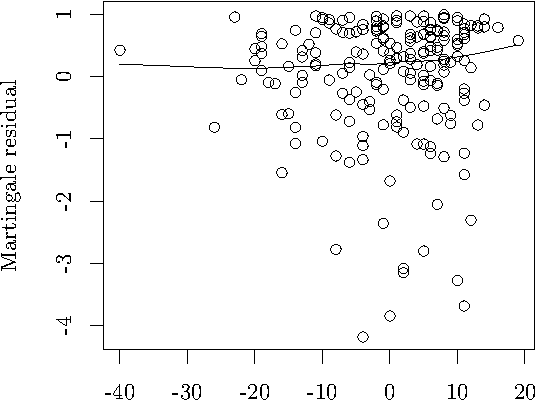
\includegraphics[width=\maxwidth]{figure/05-eda-func-form-age-1} 

}


\begin{kframe}\begin{alltt}
\hlkwd{scatter.smooth}\hlstd{(data}\hlopt{$}\hlstd{AgeCent,} \hlkwd{resid}\hlstd{(fit.cph.NoAge,} \hlkwc{type} \hlstd{=} \hlstr{"martingale"}\hlstd{),} \hlkwc{xlab} \hlstd{=} \hlstr{""}\hlstd{,} \hlkwc{ylab} \hlstd{=} \hlstr{"Martingale residual"}\hlstd{,} \hlkwc{ylim} \hlstd{=} \hlkwd{c}\hlstd{(}\hlopt{-}\hlnum{1}\hlstd{,} \hlnum{1}\hlstd{))}
\end{alltt}
\end{kframe}

{\centering 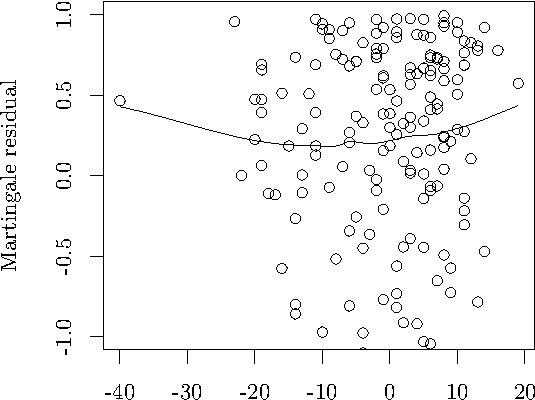
\includegraphics[width=\maxwidth]{figure/05-eda-func-form-age-2} 

}



\end{knitrout}

\begin{knitrout}
\definecolor{shadecolor}{rgb}{0.969, 0.969, 0.969}\color{fgcolor}\begin{kframe}
\begin{alltt}
\hlstd{fit.cph.NoSize} \hlkwb{=} \hlkwd{coxph}\hlstd{(}\hlkwd{Surv}\hlstd{(Time, DSD)} \hlopt{~} \hlstd{SexM} \hlopt{+} \hlstd{AgeCent} \hlopt{+} \hlstd{LocBody} \hlopt{+} \hlstd{A2} \hlopt{+} \hlstd{A4,} \hlkwc{data} \hlstd{= data)}
\hlkwd{scatter.smooth}\hlstd{(data}\hlopt{$}\hlstd{SizeCent,} \hlkwd{resid}\hlstd{(fit.cph.NoSize,} \hlkwc{type} \hlstd{=} \hlstr{"martingale"}\hlstd{),} \hlkwc{xlab} \hlstd{=} \hlstr{""}\hlstd{,} \hlkwc{ylab} \hlstd{=} \hlstr{"Martingale residual"}\hlstd{)}
\end{alltt}
\end{kframe}

{\centering 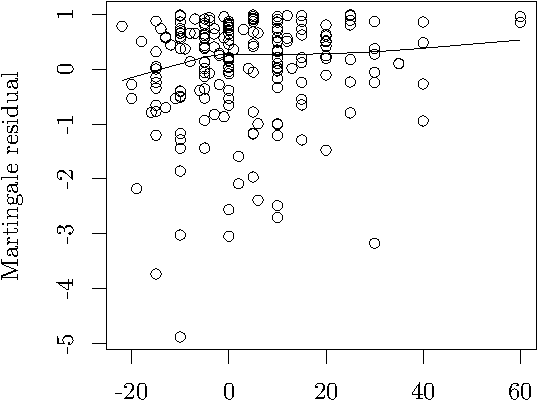
\includegraphics[width=\maxwidth]{figure/05-eda-func-form-size-1} 

}


\begin{kframe}\begin{alltt}
\hlkwd{scatter.smooth}\hlstd{(data}\hlopt{$}\hlstd{SizeCent,} \hlkwd{resid}\hlstd{(fit.cph.NoSize,} \hlkwc{type} \hlstd{=} \hlstr{"martingale"}\hlstd{),} \hlkwc{xlab} \hlstd{=} \hlstr{""}\hlstd{,} \hlkwc{ylab} \hlstd{=} \hlstr{"Martingale residual"}\hlstd{,} \hlkwc{ylim} \hlstd{=} \hlkwd{c}\hlstd{(}\hlopt{-}\hlnum{1}\hlstd{,} \hlnum{1}\hlstd{))}
\end{alltt}
\end{kframe}

{\centering 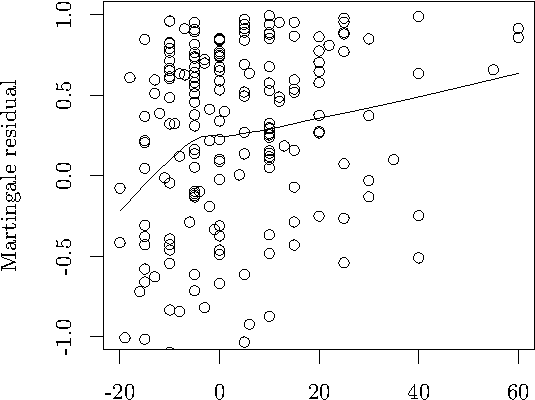
\includegraphics[width=\maxwidth]{figure/05-eda-func-form-size-2} 

}



\end{knitrout}
It looks like age has a minor nonlinear component, with a small uptick at advanced age.  Very minor though.  The size relationship appears to have a knee, close to size == 0, around which the relationship is approximately linear.

Model age as:  $AgeCent + AgeCent^2$
Model size as: $SizeCent + SizeCent I(SizeCent > 0) \equiv SizeCent + SizeCent_+$

\begin{knitrout}
\definecolor{shadecolor}{rgb}{0.969, 0.969, 0.969}\color{fgcolor}\begin{kframe}
\begin{alltt}
\hlstd{data}\hlopt{$}\hlstd{SizePlus} \hlkwb{=} \hlkwd{pmax}\hlstd{(data}\hlopt{$}\hlstd{SizeCent,} \hlnum{0}\hlstd{)}
\hlstd{data}\hlopt{$}\hlstd{AgeCent2} \hlkwb{=} \hlstd{data}\hlopt{$}\hlstd{AgeCent}\hlopt{^}\hlnum{2}
\end{alltt}
\end{kframe}
\end{knitrout}

\subsection{PH assumption: full model}
\begin{knitrout}
\definecolor{shadecolor}{rgb}{0.969, 0.969, 0.969}\color{fgcolor}\begin{kframe}
\begin{alltt}
\hlstd{fit.cph} \hlkwb{=} \hlkwd{coxph}\hlstd{(}\hlkwd{Surv}\hlstd{(Time, DSD)} \hlopt{~} \hlstd{SexM} \hlopt{+} \hlstd{AgeCent} \hlopt{+} \hlstd{AgeCent2} \hlopt{+} \hlstd{LocBody} \hlopt{+} \hlstd{SizeCent} \hlopt{+} \hlstd{SizePlus} \hlopt{+} \hlstd{A2} \hlopt{+} \hlstd{A4,} \hlkwc{data} \hlstd{= data)}
\hlkwd{cox.zph}\hlstd{(fit.cph)}
\end{alltt}
\begin{verbatim}
##                  rho    chisq      p
## SexMTRUE     0.13992  3.53766 0.0600
## AgeCent      0.02818  0.14713 0.7013
## AgeCent2     0.08589  1.33984 0.2471
## LocBodyTRUE -0.06556  0.68391 0.4082
## SizeCent    -0.05543  0.56590 0.4519
## SizePlus     0.00516  0.00482 0.9447
## A2TRUE      -0.01836  0.06213 0.8032
## A4TRUE      -0.11773  2.37767 0.1231
## GLOBAL            NA 15.64353 0.0478
\end{verbatim}
\begin{alltt}
\hlkwd{plot}\hlstd{(}\hlkwd{cox.zph}\hlstd{(fit.cph))}
\end{alltt}
\end{kframe}

{\centering 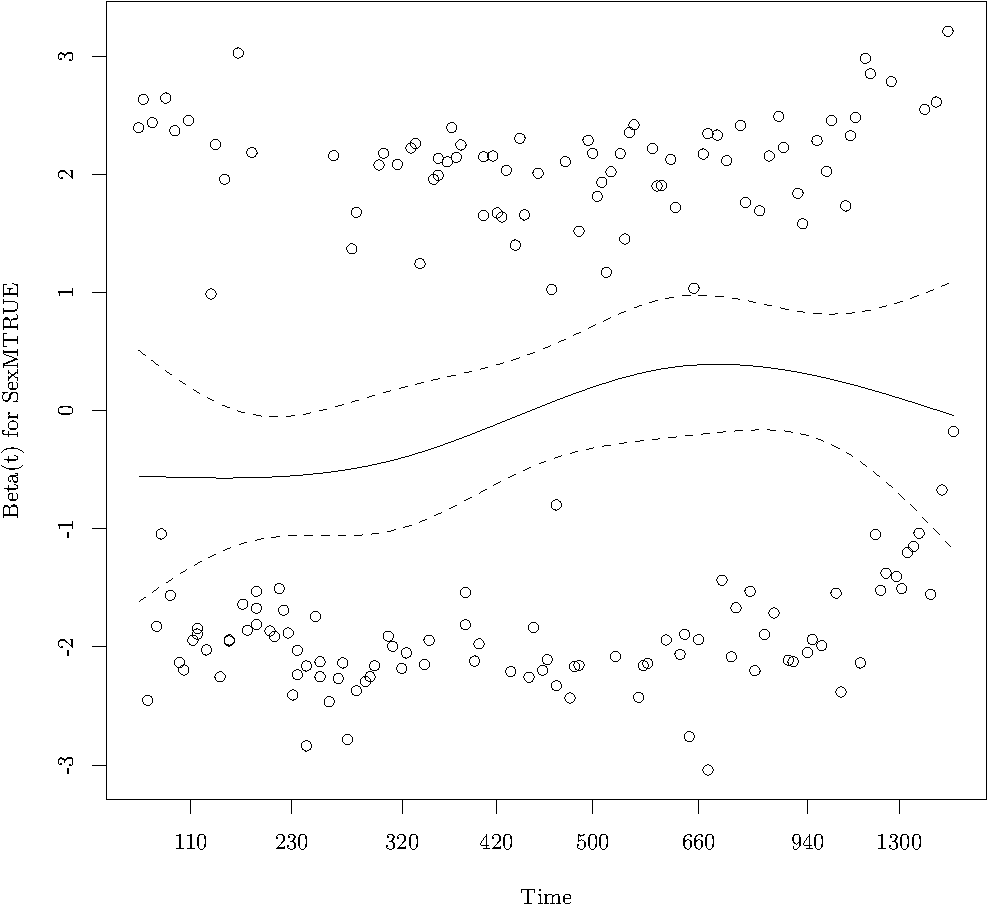
\includegraphics[width=\maxwidth]{figure/05-eda-ph-check-full-1} 

}




{\centering 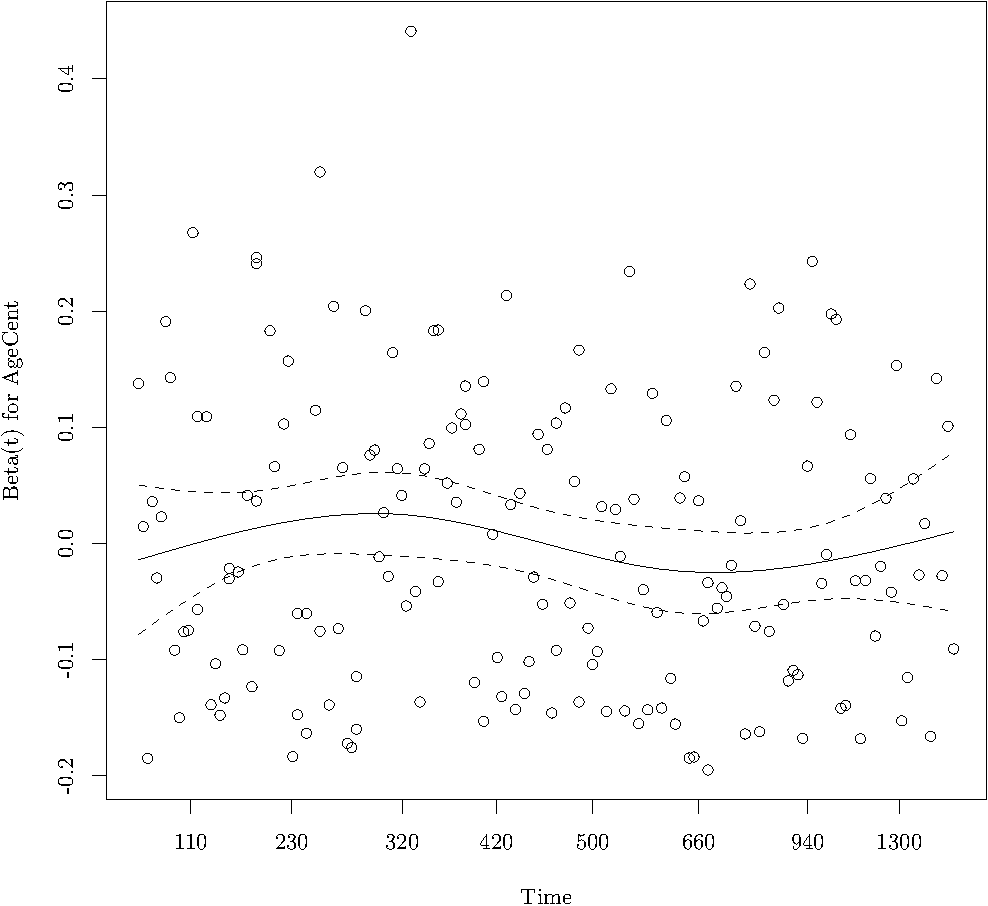
\includegraphics[width=\maxwidth]{figure/05-eda-ph-check-full-2} 

}




{\centering 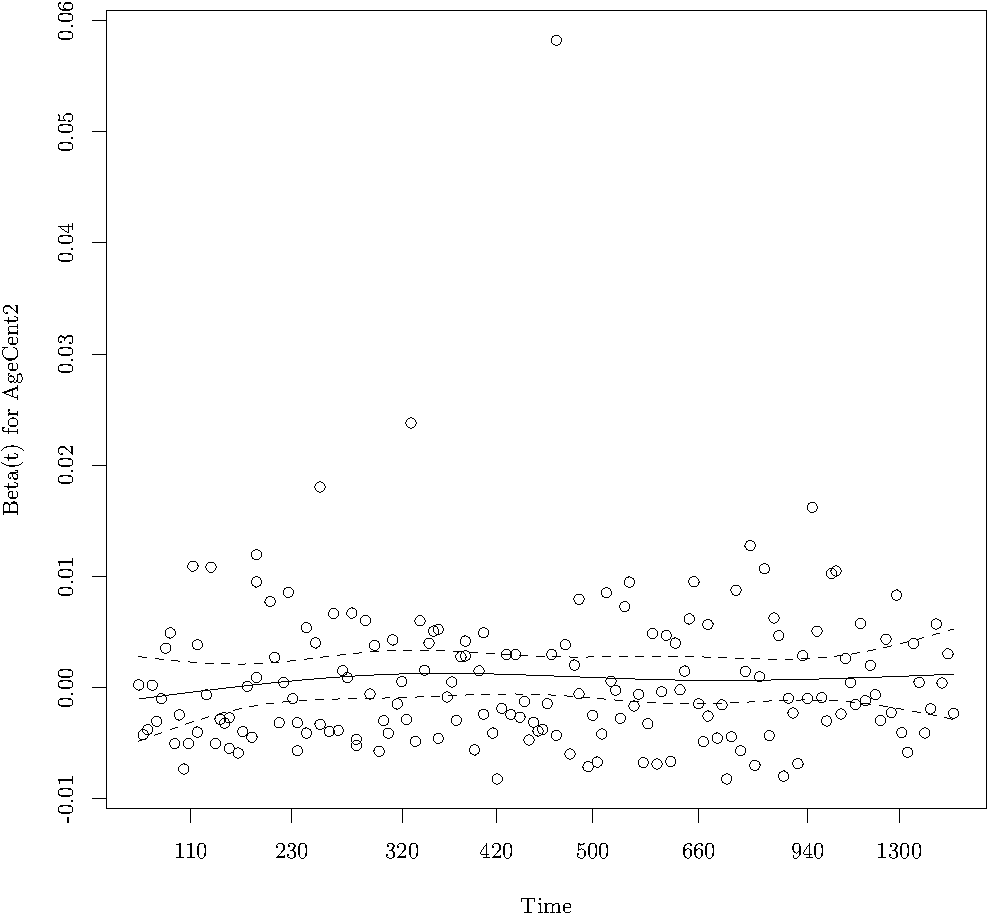
\includegraphics[width=\maxwidth]{figure/05-eda-ph-check-full-3} 

}




{\centering 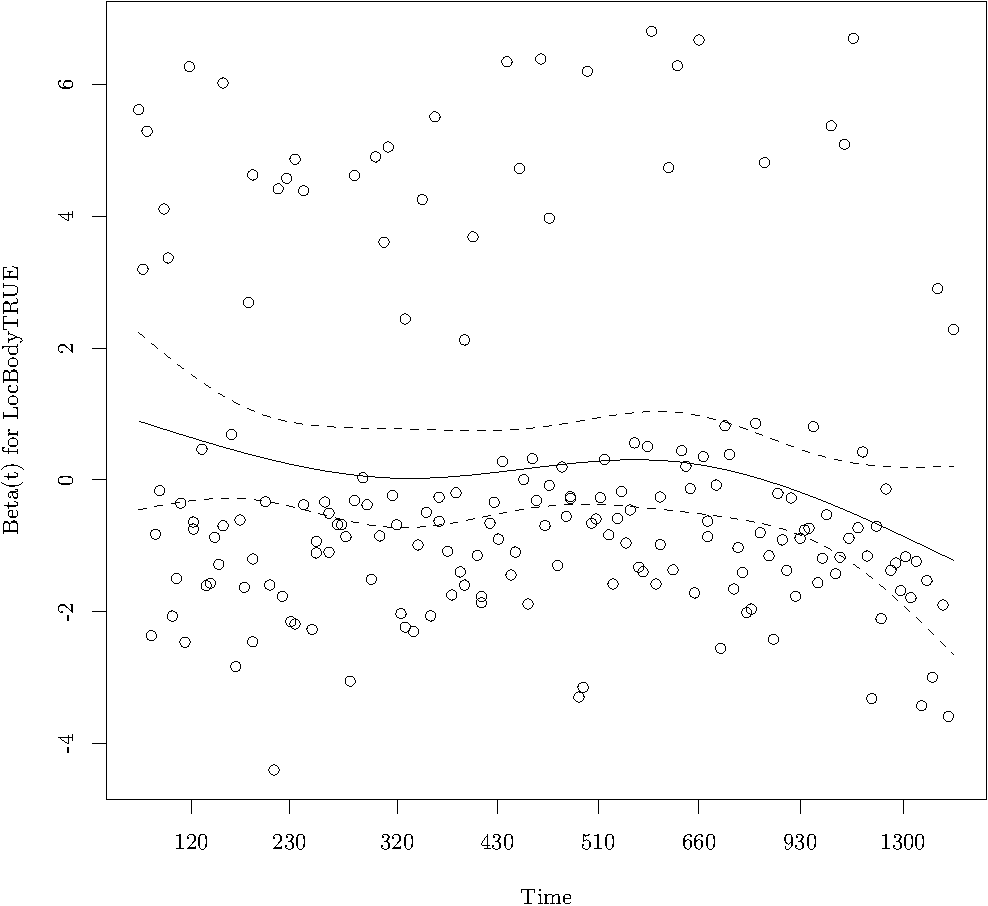
\includegraphics[width=\maxwidth]{figure/05-eda-ph-check-full-4} 

}




{\centering 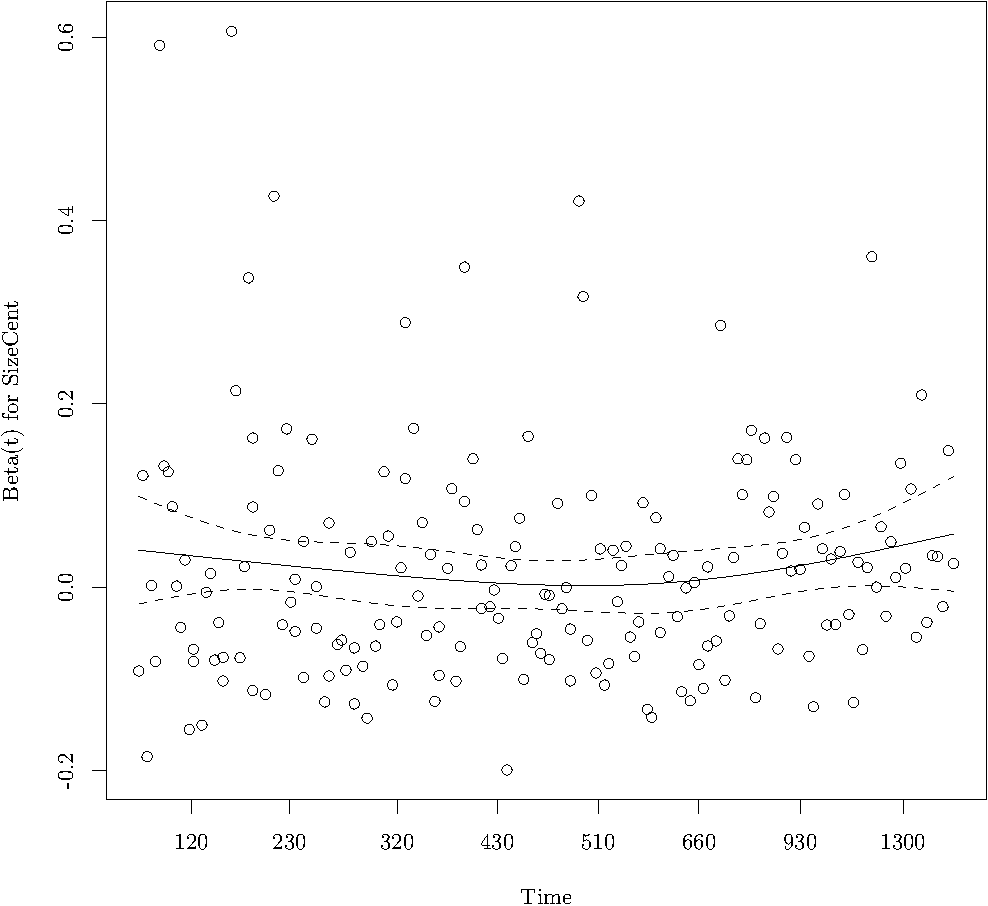
\includegraphics[width=\maxwidth]{figure/05-eda-ph-check-full-5} 

}




{\centering 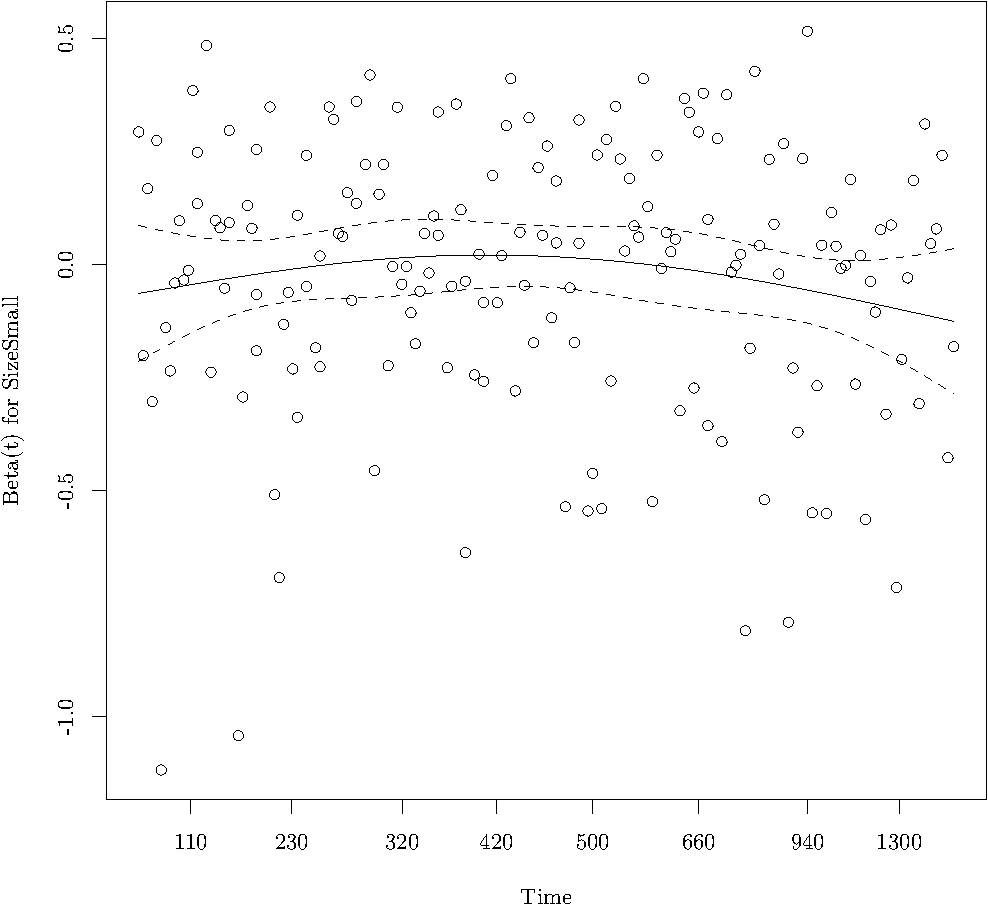
\includegraphics[width=\maxwidth]{figure/05-eda-ph-check-full-6} 

}




{\centering 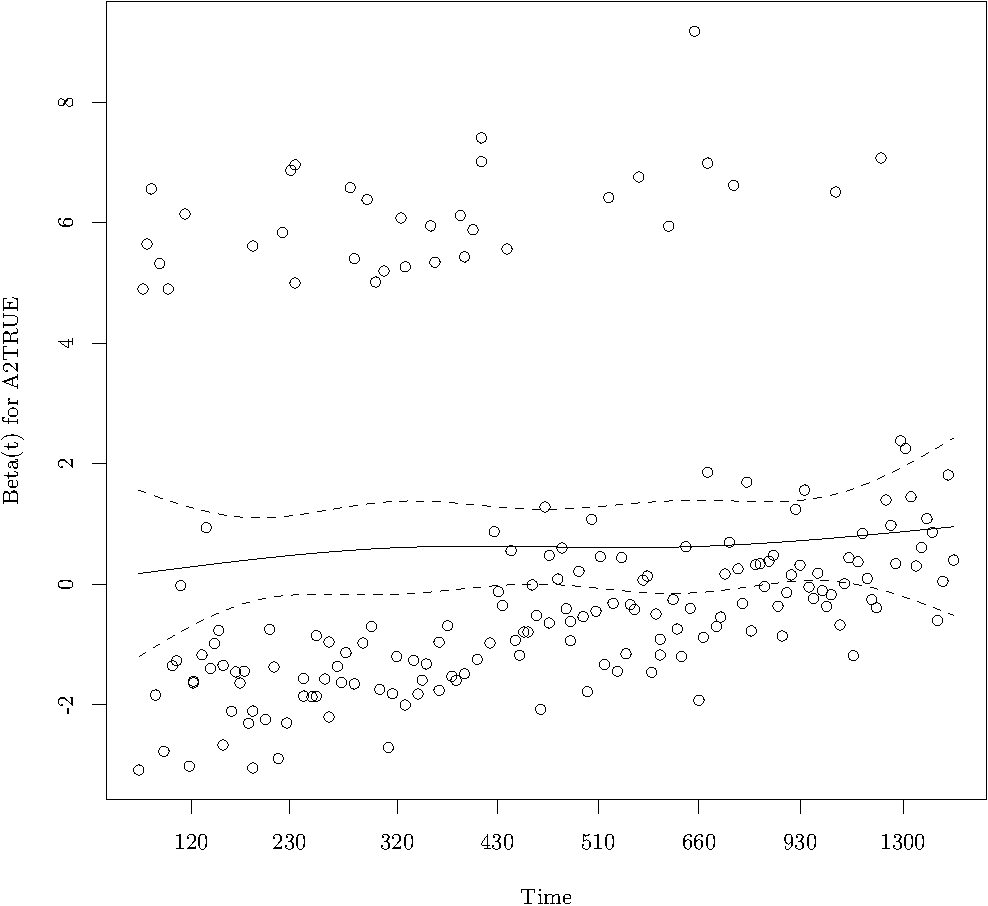
\includegraphics[width=\maxwidth]{figure/05-eda-ph-check-full-7} 

}




{\centering 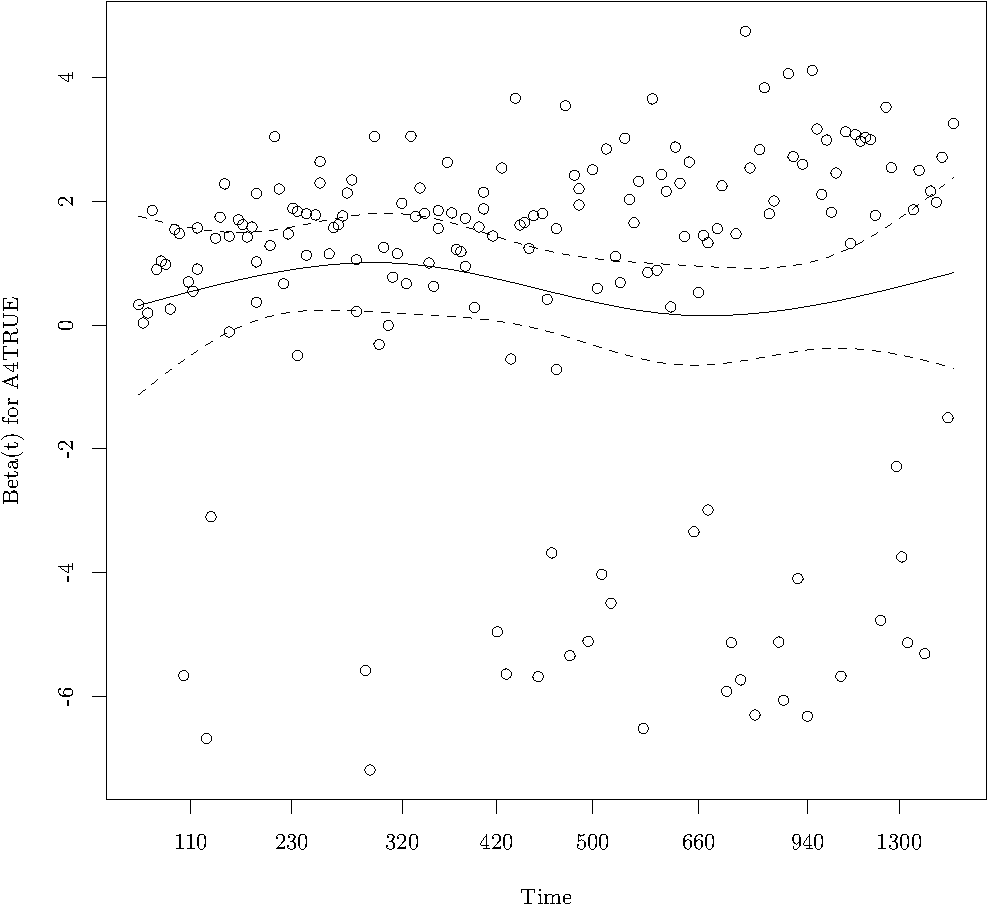
\includegraphics[width=\maxwidth]{figure/05-eda-ph-check-full-8} 

}



\end{knitrout}

\begin{knitrout}
\definecolor{shadecolor}{rgb}{0.969, 0.969, 0.969}\color{fgcolor}\begin{kframe}
\begin{alltt}
\hlstd{temp} \hlkwb{=} \hlkwa{function} \hlstd{(}\hlkwc{x}\hlstd{,} \hlkwc{resid} \hlstd{=} \hlnum{TRUE}\hlstd{,} \hlkwc{se} \hlstd{=} \hlnum{TRUE}\hlstd{,} \hlkwc{df} \hlstd{=} \hlnum{4}\hlstd{,} \hlkwc{nsmo} \hlstd{=} \hlnum{40}\hlstd{,} \hlkwc{var}\hlstd{,} \hlkwc{...}\hlstd{) \{}
    \hlstd{xx} \hlkwb{<-} \hlstd{x}\hlopt{$}\hlstd{x}
    \hlstd{yy} \hlkwb{<-} \hlstd{x}\hlopt{$}\hlstd{y}
    \hlstd{d} \hlkwb{<-} \hlkwd{nrow}\hlstd{(yy)}
    \hlstd{df} \hlkwb{<-} \hlkwd{max}\hlstd{(df)}
    \hlstd{nvar} \hlkwb{<-} \hlkwd{ncol}\hlstd{(yy)}
    \hlstd{pred.x} \hlkwb{<-} \hlkwd{seq}\hlstd{(}\hlkwc{from} \hlstd{=} \hlkwd{min}\hlstd{(xx),} \hlkwc{to} \hlstd{=} \hlkwd{max}\hlstd{(xx),} \hlkwc{length} \hlstd{= nsmo)}
    \hlstd{temp} \hlkwb{<-} \hlkwd{c}\hlstd{(pred.x, xx)}
    \hlstd{lmat} \hlkwb{<-} \hlkwd{ns}\hlstd{(temp,} \hlkwc{df} \hlstd{= df,} \hlkwc{intercept} \hlstd{=} \hlnum{TRUE}\hlstd{)}
    \hlstd{pmat} \hlkwb{<-} \hlstd{lmat[}\hlnum{1}\hlopt{:}\hlstd{nsmo, ]}
    \hlstd{xmat} \hlkwb{<-} \hlstd{lmat[}\hlopt{-}\hlstd{(}\hlnum{1}\hlopt{:}\hlstd{nsmo), ]}
    \hlstd{qmat} \hlkwb{<-} \hlkwd{qr}\hlstd{(xmat)}
    \hlkwa{if} \hlstd{(qmat}\hlopt{$}\hlstd{rank} \hlopt{<} \hlstd{df)}
        \hlkwd{stop}\hlstd{(}\hlstr{"Spline fit is singular, try a smaller degrees of freedom"}\hlstd{)}
    \hlkwa{if} \hlstd{(se) \{}
        \hlstd{bk} \hlkwb{<-} \hlkwd{backsolve}\hlstd{(qmat}\hlopt{$}\hlstd{qr[}\hlnum{1}\hlopt{:}\hlstd{df,} \hlnum{1}\hlopt{:}\hlstd{df],} \hlkwd{diag}\hlstd{(df))}
        \hlstd{xtx} \hlkwb{<-} \hlstd{bk} \hlopt \hlkwd{t}\hlstd{(bk)}
        \hlstd{seval} \hlkwb{<-} \hlstd{d} \hlopt{*} \hlstd{((pmat} \hlopt \hlstd{xtx)} \hlopt{*} \hlstd{pmat)} \hlopt \hlkwd{rep}\hlstd{(}\hlnum{1}\hlstd{, df)}
    \hlstd{\}}
    \hlstd{ylab} \hlkwb{<-} \hlkwd{paste}\hlstd{(}\hlstr{"Beta(t) for"}\hlstd{,} \hlkwd{dimnames}\hlstd{(yy)[[}\hlnum{2}\hlstd{]])}
    \hlkwa{if} \hlstd{(}\hlkwd{missing}\hlstd{(var))}
        \hlstd{var} \hlkwb{<-} \hlnum{1}\hlopt{:}\hlstd{nvar}
    \hlkwa{else} \hlstd{\{}
        \hlkwa{if} \hlstd{(}\hlkwd{is.character}\hlstd{(var))}
            \hlstd{var} \hlkwb{<-} \hlkwd{match}\hlstd{(var,} \hlkwd{dimnames}\hlstd{(yy)[[}\hlnum{2}\hlstd{]])}
        \hlkwa{if} \hlstd{(}\hlkwd{any}\hlstd{(}\hlkwd{is.na}\hlstd{(var))} \hlopt{||} \hlkwd{max}\hlstd{(var)} \hlopt{>} \hlstd{nvar} \hlopt{||} \hlkwd{min}\hlstd{(var)} \hlopt{<}
            \hlnum{1}\hlstd{)}
            \hlkwd{stop}\hlstd{(}\hlstr{"Invalid variable requested"}\hlstd{)}
    \hlstd{\}}
    \hlkwa{if} \hlstd{(x}\hlopt{$}\hlstd{transform} \hlopt{==} \hlstr{"log"}\hlstd{) \{}
        \hlstd{xx} \hlkwb{<-} \hlkwd{exp}\hlstd{(xx)}
        \hlstd{pred.x} \hlkwb{<-} \hlkwd{exp}\hlstd{(pred.x)}
    \hlstd{\}}
    \hlkwa{else if} \hlstd{(x}\hlopt{$}\hlstd{transform} \hlopt{!=} \hlstr{"identity"}\hlstd{) \{}
        \hlstd{xtime} \hlkwb{<-} \hlkwd{as.numeric}\hlstd{(}\hlkwd{dimnames}\hlstd{(yy)[[}\hlnum{1}\hlstd{]])}
        \hlstd{indx} \hlkwb{<-} \hlopt{!}\hlkwd{duplicated}\hlstd{(xx)}
        \hlstd{apr1} \hlkwb{<-} \hlkwd{approx}\hlstd{(xx[indx], xtime[indx],} \hlkwd{seq}\hlstd{(}\hlkwd{min}\hlstd{(xx),} \hlkwd{max}\hlstd{(xx),}
            \hlkwc{length} \hlstd{=} \hlnum{17}\hlstd{)[}\hlnum{2} \hlopt{*} \hlstd{(}\hlnum{1}\hlopt{:}\hlnum{8}\hlstd{)])}
        \hlstd{temp} \hlkwb{<-} \hlkwd{signif}\hlstd{(apr1}\hlopt{$}\hlstd{y,} \hlnum{2}\hlstd{)}
        \hlstd{apr2} \hlkwb{<-} \hlkwd{approx}\hlstd{(xtime[indx], xx[indx], temp)}
        \hlstd{xaxisval} \hlkwb{<-} \hlstd{apr2}\hlopt{$}\hlstd{y}
        \hlstd{xaxislab} \hlkwb{<-} \hlkwd{rep}\hlstd{(}\hlstr{""}\hlstd{,} \hlnum{8}\hlstd{)}
        \hlkwa{for} \hlstd{(i} \hlkwa{in} \hlnum{1}\hlopt{:}\hlnum{8}\hlstd{) xaxislab[i]} \hlkwb{<-} \hlkwd{format}\hlstd{(temp[i])}
    \hlstd{\}}
    \hlkwa{for} \hlstd{(i} \hlkwa{in} \hlstd{var) \{}
        \hlstd{y} \hlkwb{<-} \hlstd{yy[, i]}
        \hlstd{yhat} \hlkwb{<-} \hlstd{pmat} \hlopt \hlkwd{qr.coef}\hlstd{(qmat, y)}
        \hlkwa{if} \hlstd{(resid)}
            \hlstd{yr} \hlkwb{<-} \hlkwd{range}\hlstd{(yhat, y)}
        \hlkwa{else} \hlstd{yr} \hlkwb{<-} \hlkwd{range}\hlstd{(yhat)}
        \hlkwa{if} \hlstd{(se) \{}
            \hlstd{temp} \hlkwb{<-} \hlnum{2} \hlopt{*} \hlkwd{sqrt}\hlstd{(x}\hlopt{$}\hlstd{var[i, i]} \hlopt{*} \hlstd{seval)}
            \hlstd{yup} \hlkwb{<-} \hlstd{yhat} \hlopt{+} \hlstd{temp}
            \hlstd{ylow} \hlkwb{<-} \hlstd{yhat} \hlopt{-} \hlstd{temp}
            \hlstd{yr} \hlkwb{<-} \hlkwd{range}\hlstd{(yr, yup, ylow)}
        \hlstd{\}}
        \hlkwa{if} \hlstd{(x}\hlopt{$}\hlstd{transform} \hlopt{==} \hlstr{"identity"}\hlstd{)}
            \hlkwd{plot}\hlstd{(}\hlkwd{range}\hlstd{(xx), yr,} \hlkwc{type} \hlstd{=} \hlstr{"n"}\hlstd{, ...)}
        \hlkwa{else if} \hlstd{(x}\hlopt{$}\hlstd{transform} \hlopt{==} \hlstr{"log"}\hlstd{)}
            \hlkwd{plot}\hlstd{(}\hlkwd{range}\hlstd{(xx), yr,} \hlkwc{type} \hlstd{=} \hlstr{"n"}\hlstd{,} \hlkwc{log} \hlstd{=} \hlstr{"x"}\hlstd{, ...)}
        \hlkwa{else} \hlstd{\{}
            \hlkwd{plot}\hlstd{(}\hlkwd{range}\hlstd{(xx), yr,} \hlkwc{type} \hlstd{=} \hlstr{"n"}\hlstd{,} \hlkwc{axes} \hlstd{=} \hlnum{FALSE}\hlstd{, ...)}
            \hlkwd{axis}\hlstd{(}\hlnum{1}\hlstd{, xaxisval, xaxislab)}
            \hlkwd{axis}\hlstd{(}\hlnum{2}\hlstd{)}
            \hlkwd{box}\hlstd{()}
        \hlstd{\}}
        \hlkwa{if} \hlstd{(resid)}
            \hlkwd{points}\hlstd{(xx, y)}
        \hlkwd{lines}\hlstd{(pred.x, yhat)}
        \hlkwa{if} \hlstd{(se) \{}
            \hlkwd{lines}\hlstd{(pred.x, yup,} \hlkwc{lty} \hlstd{=} \hlnum{2}\hlstd{)}
            \hlkwd{lines}\hlstd{(pred.x, ylow,} \hlkwc{lty} \hlstd{=} \hlnum{2}\hlstd{)}
        \hlstd{\}}
    \hlstd{\}}
\hlstd{\}}

\hlkwd{temp}\hlstd{(}\hlkwd{cox.zph}\hlstd{(fit.cph),} \hlkwc{var} \hlstd{=} \hlnum{1}\hlstd{,} \hlkwc{ylab} \hlstd{=} \hlstr{"Scaled Schoenfeld residual for patient sex"}\hlstd{,} \hlkwc{xlab} \hlstd{=} \hlstr{"Time"}\hlstd{)}
\hlkwd{abline}\hlstd{(}\hlkwc{h} \hlstd{=} \hlnum{0}\hlstd{,} \hlkwc{lty} \hlstd{=} \hlstr{"dotted"}\hlstd{)}
\end{alltt}
\end{kframe}

{\centering 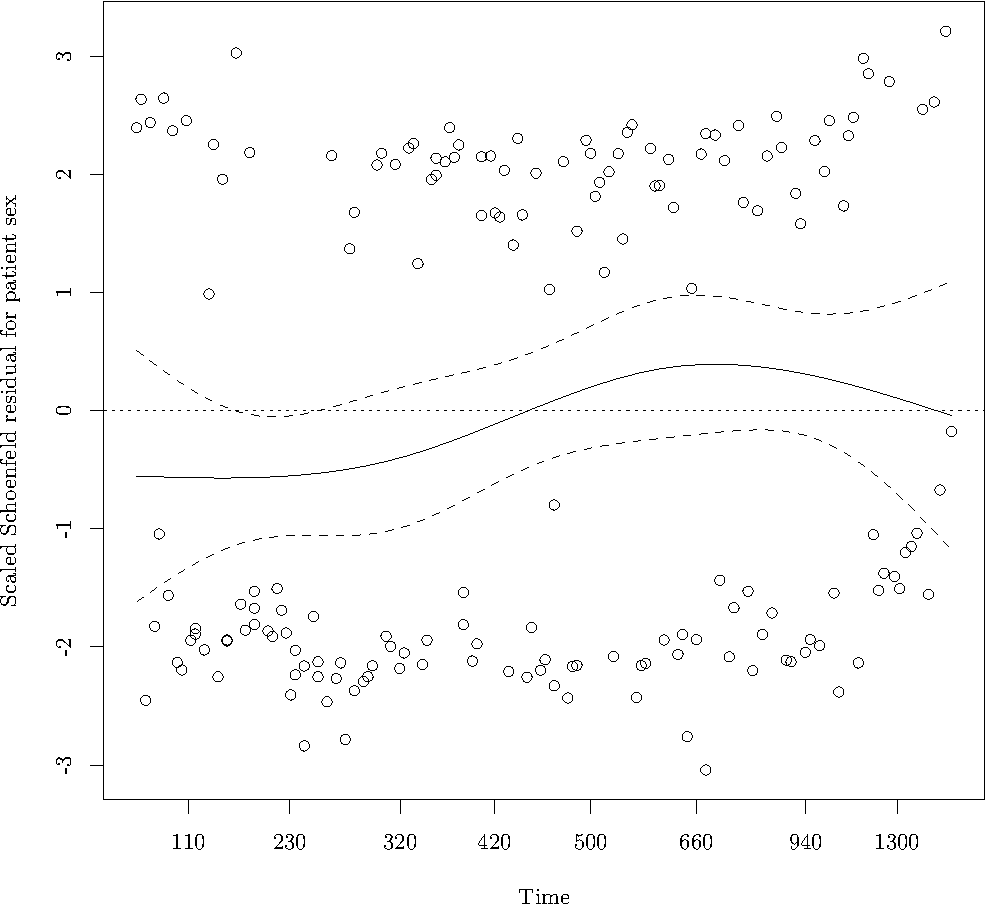
\includegraphics[width=\maxwidth]{figure/05-eda-ph-check-full-sexplot-1} 

}



\end{knitrout}


Looks like there's a violation of CPH with gender.  Not unexpected.  First check whether there is any evidence of gender interaction.
\begin{knitrout}
\definecolor{shadecolor}{rgb}{0.969, 0.969, 0.969}\color{fgcolor}\begin{kframe}
\begin{alltt}
\hlkwd{anova}\hlstd{(}\hlkwd{coxph}\hlstd{(}\hlkwd{Surv}\hlstd{(Time, DSD)} \hlopt{~} \hlstd{SexM}\hlopt{*}\hlstd{(AgeCent} \hlopt{+} \hlstd{AgeCent2} \hlopt{+} \hlstd{LocBody} \hlopt{+} \hlstd{SizeCent} \hlopt{+} \hlstd{SizePlus} \hlopt{+} \hlstd{A2} \hlopt{+} \hlstd{A4),} \hlkwc{data} \hlstd{= data))}
\end{alltt}
\begin{verbatim}
## Analysis of Deviance Table
##  Cox model: response is Surv(Time, DSD)
## Terms added sequentially (first to last)
## 
##               loglik Chisq Df Pr(>|Chi|)
## NULL            -781                    
## SexM            -781  0.20  1     0.6574
## AgeCent         -781  0.49  1     0.4835
## AgeCent2        -780  1.62  1     0.2029
## LocBody         -777  6.69  1     0.0097
## SizeCent        -774  4.83  1     0.0280
## SizePlus        -772  5.07  1     0.0244
## A2              -769  5.14  1     0.0234
## A4              -767  4.79  1     0.0286
## SexM:AgeCent    -767  0.00  1     0.9726
## SexM:AgeCent2   -767  0.15  1     0.7016
## SexM:LocBody    -767  0.02  1     0.8955
## SexM:SizeCent   -766  1.85  1     0.1733
## SexM:SizePlus   -765  0.93  1     0.3350
## SexM:A2         -764  2.24  1     0.1343
## SexM:A4         -764  0.05  1     0.8151
\end{verbatim}
\end{kframe}
\end{knitrout}
Nope, good.  We're not interested in gender effects so just stratify.

\begin{knitrout}
\definecolor{shadecolor}{rgb}{0.969, 0.969, 0.969}\color{fgcolor}\begin{kframe}
\begin{alltt}
\hlstd{fit.cph} \hlkwb{=} \hlkwd{coxph}\hlstd{(}\hlkwd{Surv}\hlstd{(Time, DSD)} \hlopt{~} \hlkwd{strata}\hlstd{(SexM)} \hlopt{+} \hlstd{AgeCent} \hlopt{+} \hlstd{AgeCent2} \hlopt{+} \hlstd{LocBody} \hlopt{+} \hlstd{SizeCent} \hlopt{+} \hlstd{SizePlus} \hlopt{+} \hlstd{A2} \hlopt{+} \hlstd{A4,} \hlkwc{data} \hlstd{= data)}
\hlkwd{cox.zph}\hlstd{(fit.cph)}
\end{alltt}
\begin{verbatim}
##                 rho   chisq      p
## AgeCent      0.0198  0.0726 0.7876
## AgeCent2     0.0855  1.3234 0.2500
## LocBodyTRUE -0.0716  0.7957 0.3724
## SizeCent    -0.0676  0.8362 0.3605
## SizePlus     0.0152  0.0412 0.8392
## A2TRUE      -0.0146  0.0392 0.8431
## A4TRUE      -0.1152  2.2494 0.1337
## GLOBAL           NA 12.0728 0.0982
\end{verbatim}
\begin{alltt}
\hlkwd{plot}\hlstd{(}\hlkwd{cox.zph}\hlstd{(fit.cph))}
\end{alltt}
\end{kframe}

{\centering 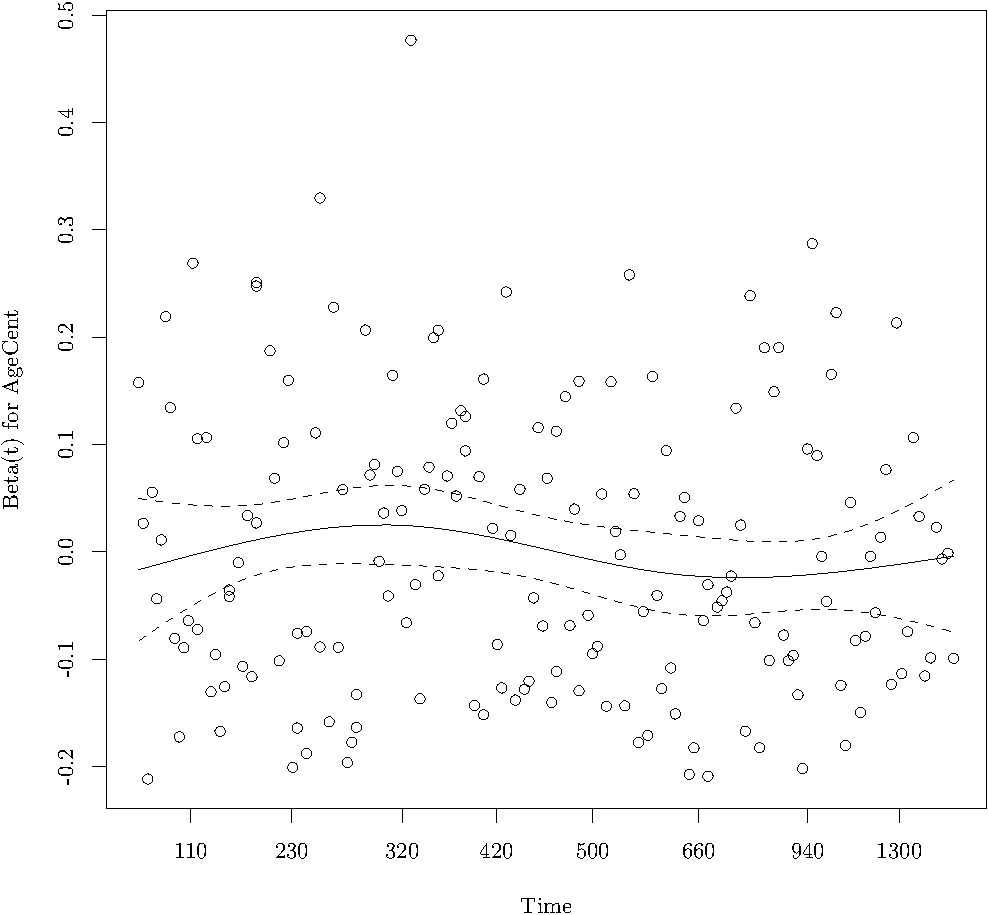
\includegraphics[width=\maxwidth]{figure/05-eda-ph-check-full-3-1} 

}




{\centering 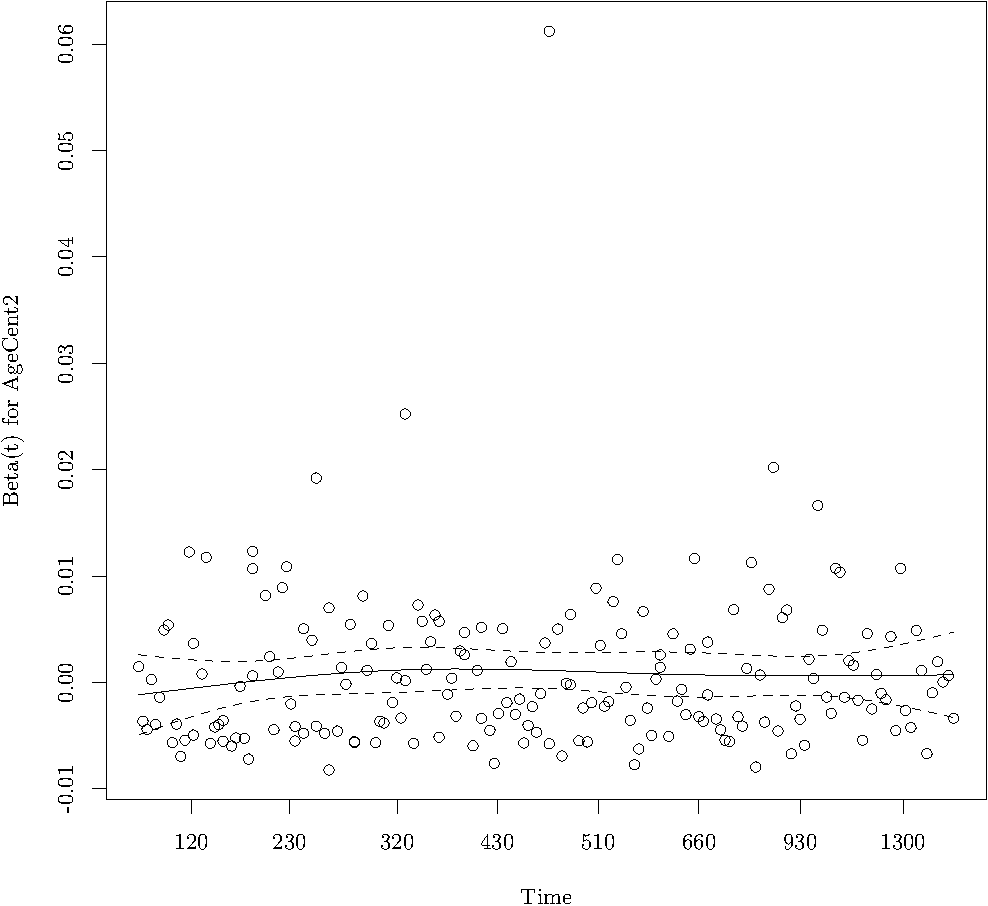
\includegraphics[width=\maxwidth]{figure/05-eda-ph-check-full-3-2} 

}




{\centering 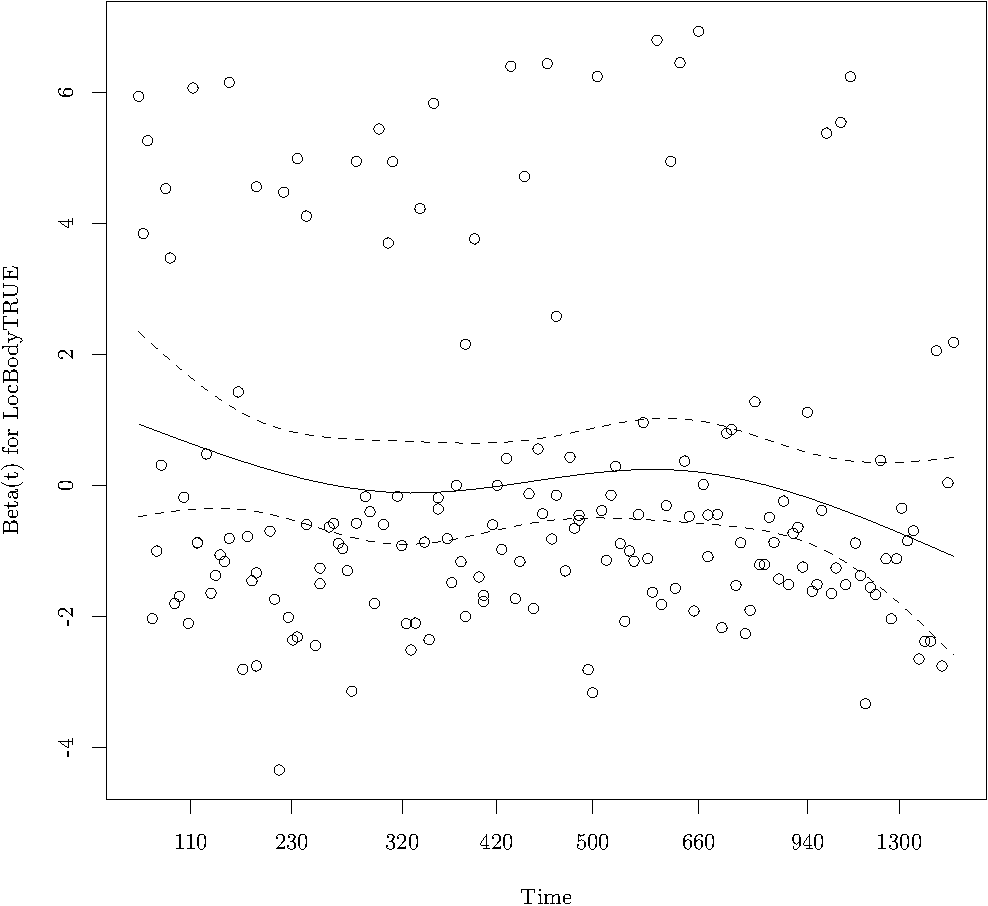
\includegraphics[width=\maxwidth]{figure/05-eda-ph-check-full-3-3} 

}




{\centering 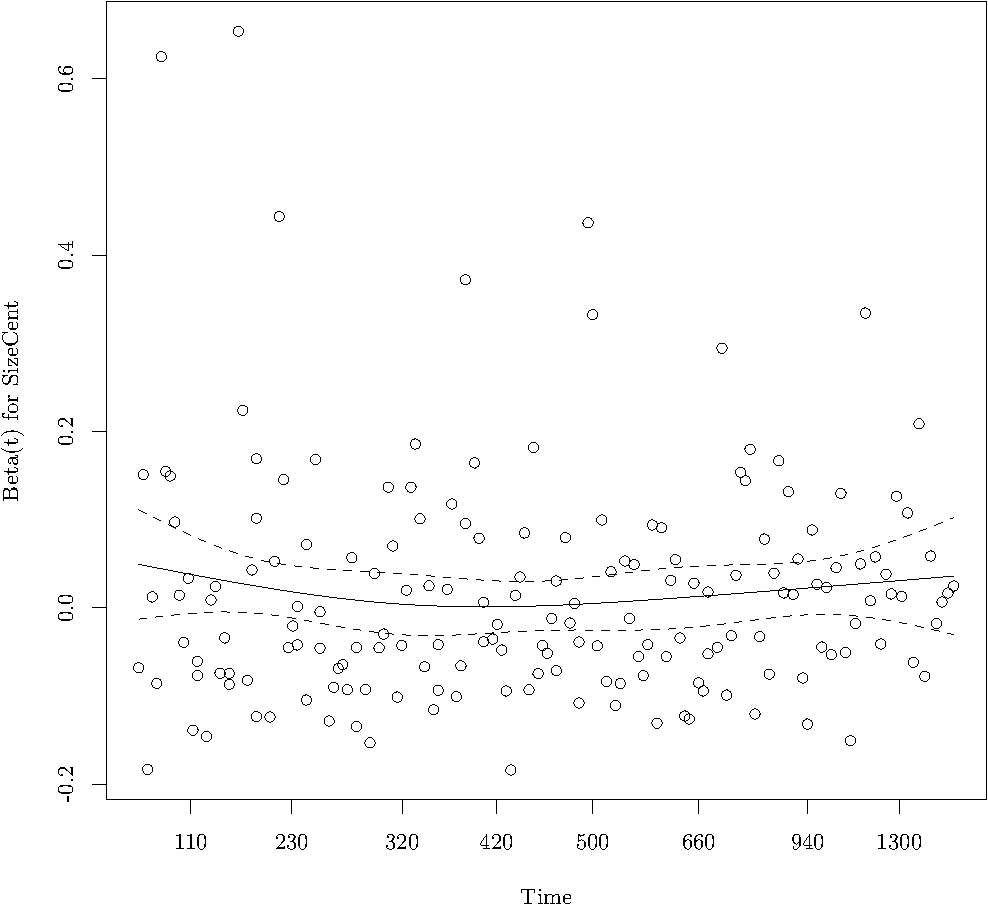
\includegraphics[width=\maxwidth]{figure/05-eda-ph-check-full-3-4} 

}




{\centering 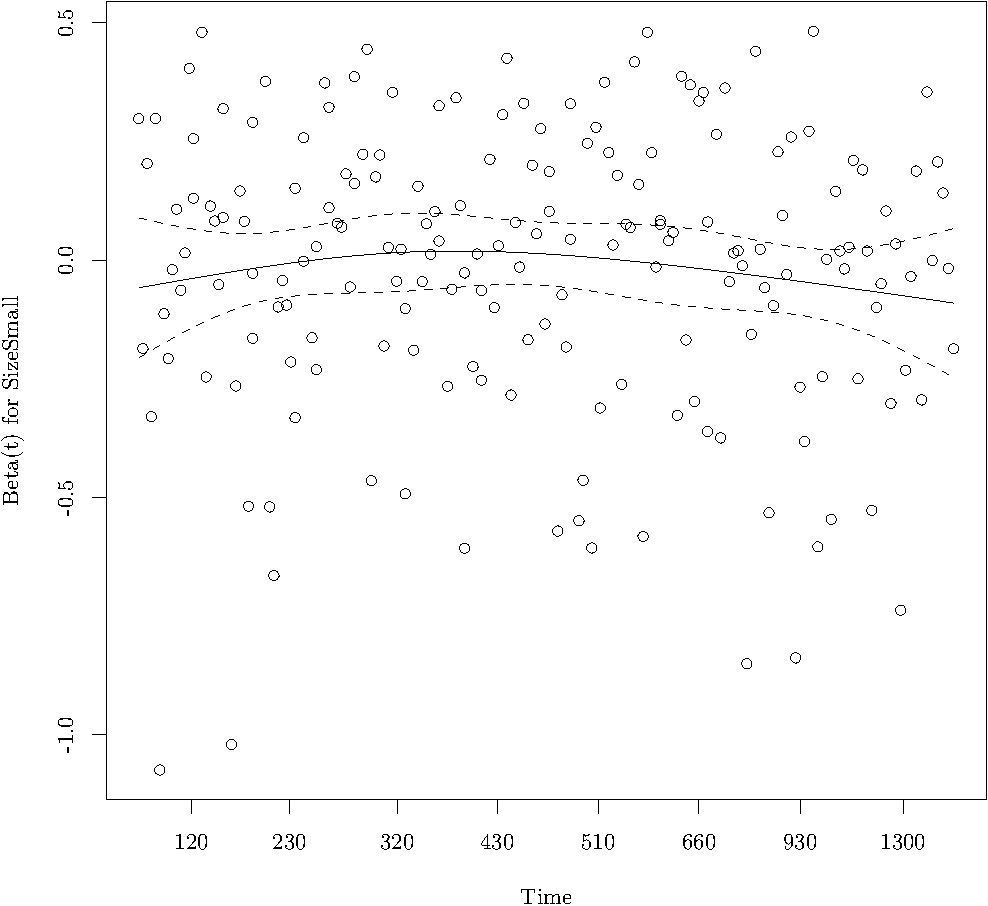
\includegraphics[width=\maxwidth]{figure/05-eda-ph-check-full-3-5} 

}




{\centering 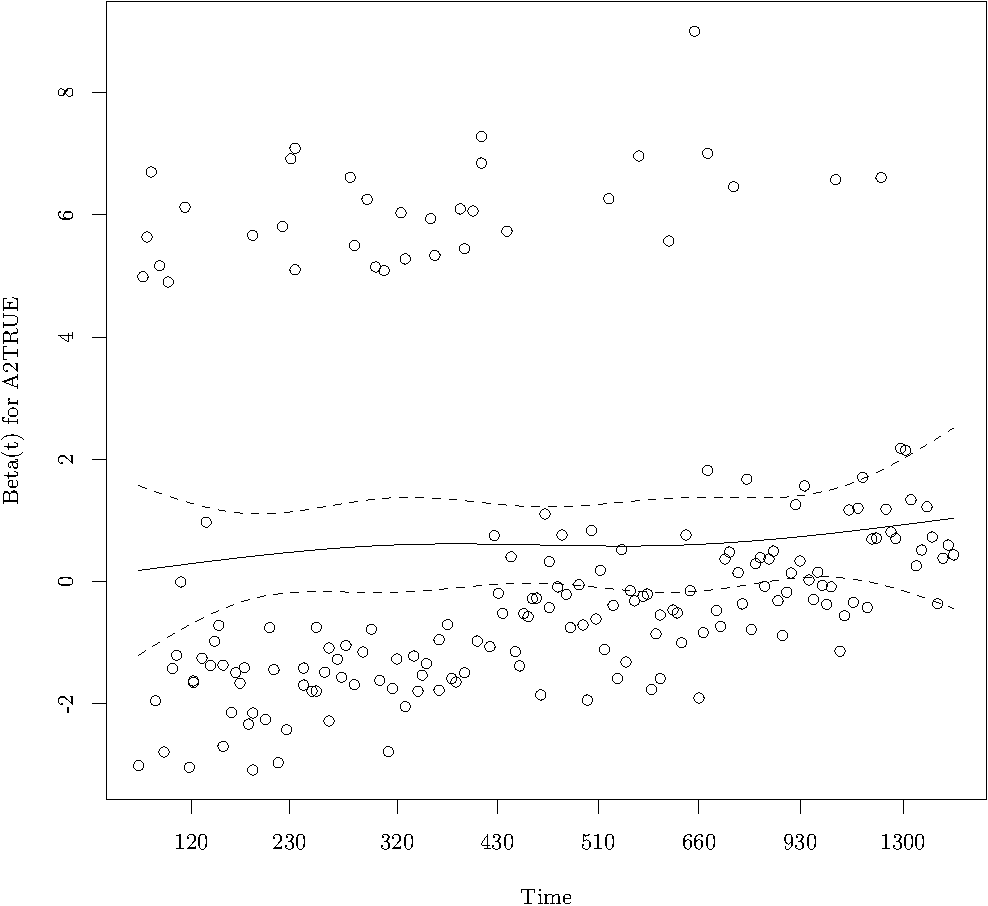
\includegraphics[width=\maxwidth]{figure/05-eda-ph-check-full-3-6} 

}




{\centering 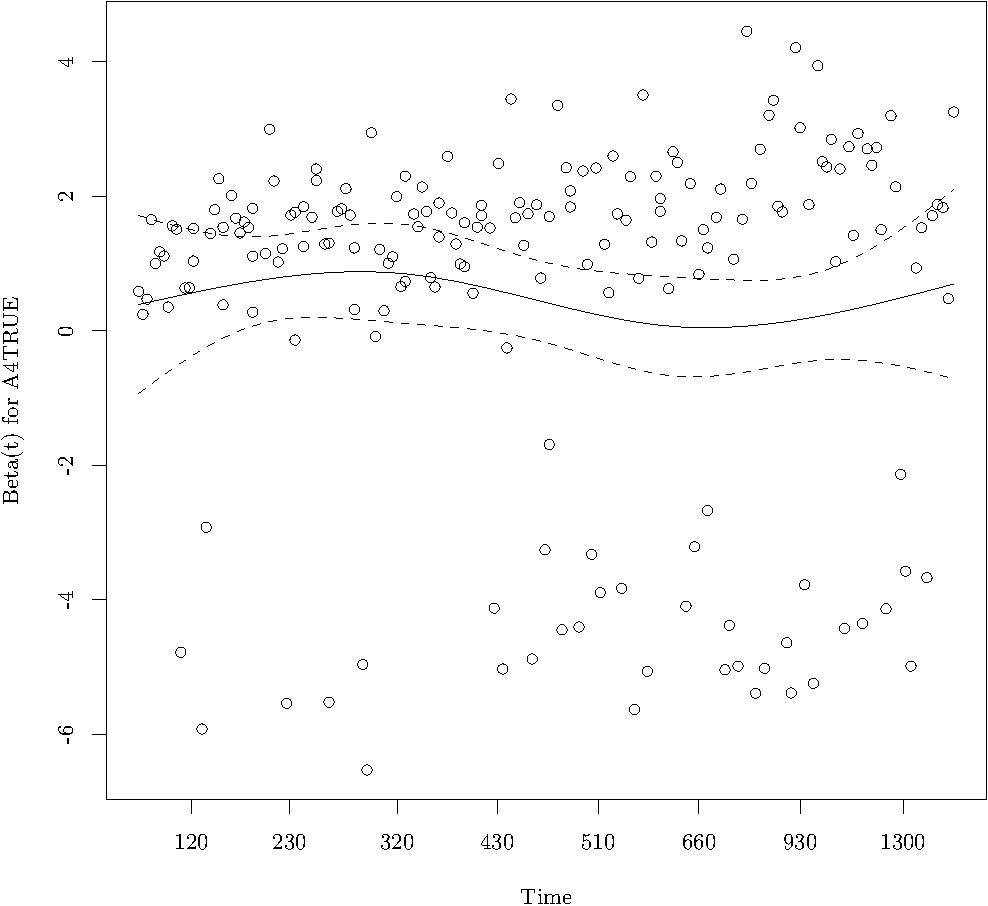
\includegraphics[width=\maxwidth]{figure/05-eda-ph-check-full-3-7} 

}



\end{knitrout}

Looks good.  Slight snifter with age but I'm not particularly concerned.
Split into age groups and do KM plots to verify.
\begin{knitrout}
\definecolor{shadecolor}{rgb}{0.969, 0.969, 0.969}\color{fgcolor}\begin{kframe}
\begin{alltt}
\hlstd{temp.age} \hlkwb{=} \hlkwd{cut}\hlstd{(data}\hlopt{$}\hlstd{AgeCent,} \hlnum{4}\hlstd{)}
\hlstd{temp} \hlkwb{=} \hlkwd{survfit}\hlstd{(}\hlkwd{Surv}\hlstd{(Time, DSD)} \hlopt{~} \hlstd{temp.age, data)}
\hlkwd{ggplot}\hlstd{(}\hlkwd{data.frame}\hlstd{(}\hlkwc{surv} \hlstd{= temp}\hlopt{$}\hlstd{surv,} \hlkwc{time} \hlstd{= temp}\hlopt{$}\hlstd{time,} \hlkwc{age} \hlstd{=} \hlkwd{rep}\hlstd{(}\hlkwd{names}\hlstd{(temp}\hlopt{$}\hlstd{strata), temp}\hlopt{$}\hlstd{strata)),} \hlkwd{aes}\hlstd{(}\hlkwc{y} \hlstd{=} \hlkwd{log}\hlstd{(}\hlopt{-}\hlkwd{log}\hlstd{(surv)),} \hlkwc{x} \hlstd{=} \hlkwd{log}\hlstd{(time),} \hlkwc{col} \hlstd{= age))} \hlopt{+} \hlkwd{geom_line}\hlstd{()}
\end{alltt}
\end{kframe}

{\centering 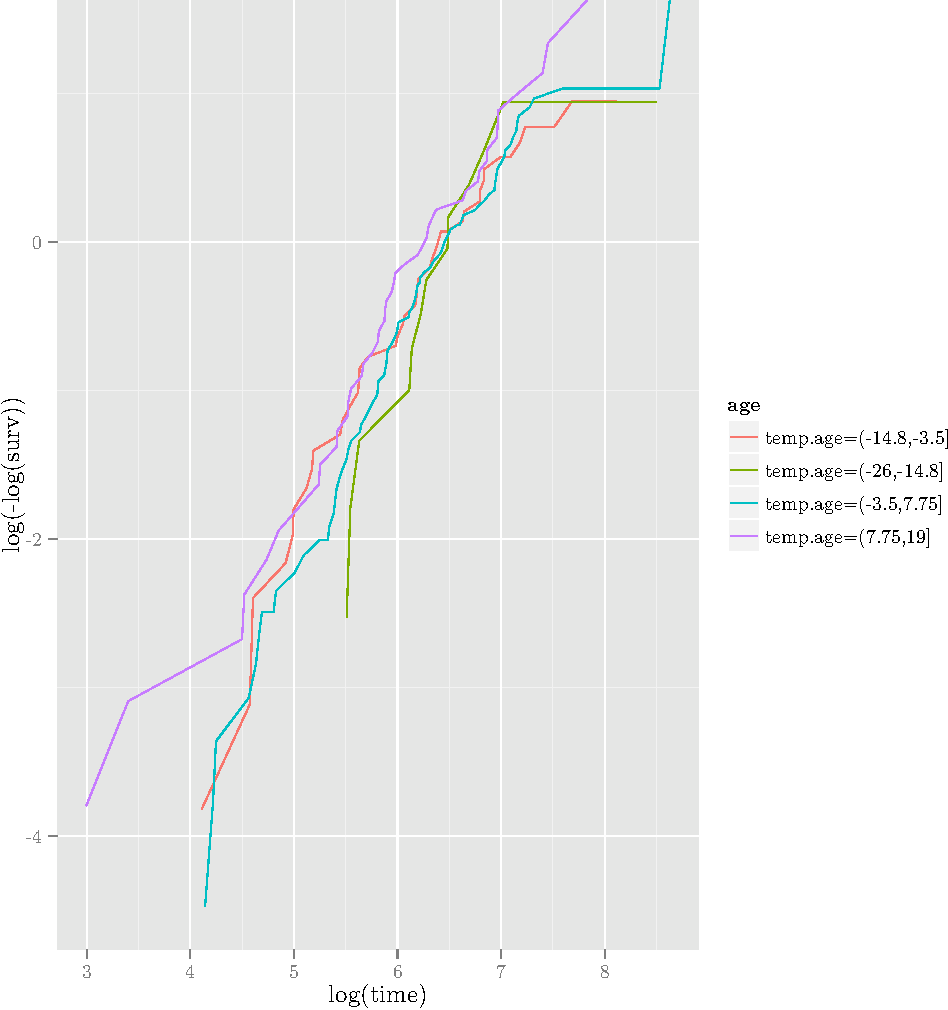
\includegraphics[width=\maxwidth]{figure/05-eda-ph-check-full-age-1} 

}



\end{knitrout}
Not perfect but it'll do.


\subsection{Outliers: full model}
Look at deviance residuals, both marginally and stratified by major subgroups.
\begin{knitrout}
\definecolor{shadecolor}{rgb}{0.969, 0.969, 0.969}\color{fgcolor}\begin{kframe}
\begin{alltt}
\hlkwd{plot}\hlstd{(}\hlkwd{resid}\hlstd{(fit.cph,} \hlkwc{type} \hlstd{=} \hlstr{"deviance"}\hlstd{))}
\hlkwd{abline}\hlstd{(}\hlkwc{h} \hlstd{=} \hlkwd{c}\hlstd{(}\hlopt{-}\hlnum{2.5}\hlstd{,} \hlnum{2.5}\hlstd{))}
\end{alltt}
\end{kframe}

{\centering 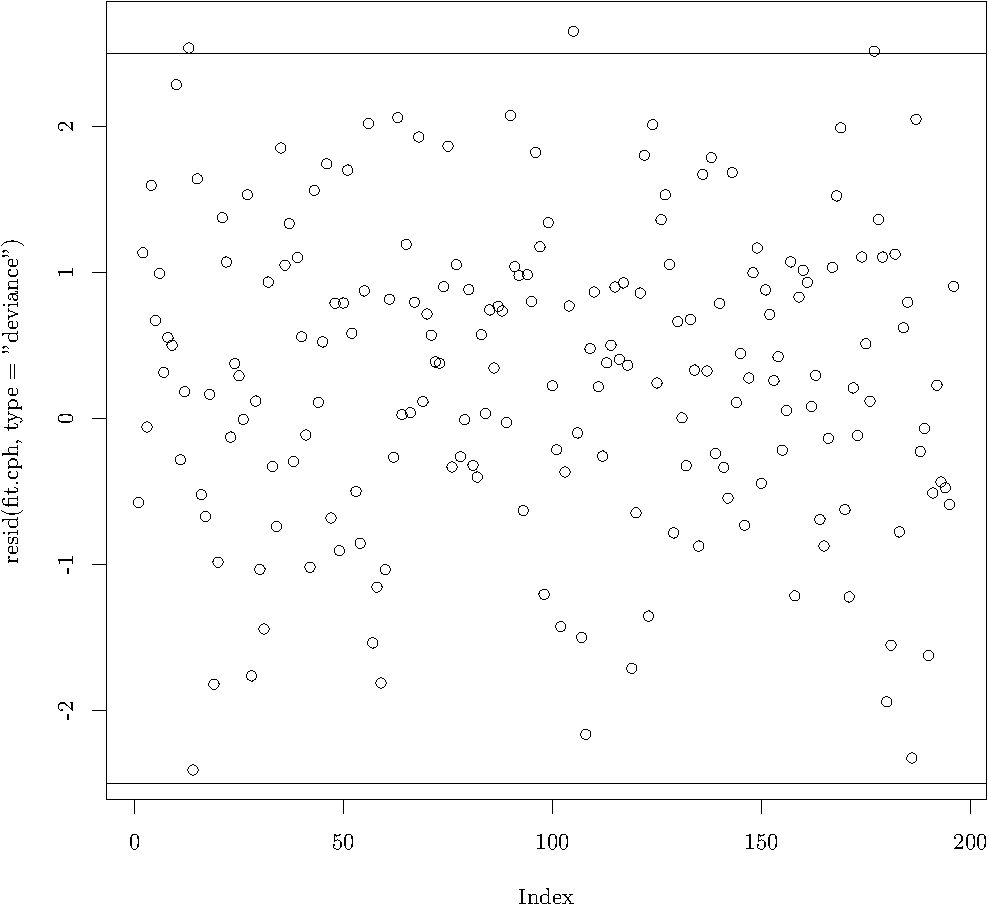
\includegraphics[width=\maxwidth]{figure/05-eda-outliers-full-1} 

}


\begin{kframe}\begin{alltt}
\hlstd{temp.ord} \hlkwb{=} \hlkwd{order}\hlstd{(data}\hlopt{$}\hlstd{SexM, data}\hlopt{$}\hlstd{A2, data}\hlopt{$}\hlstd{A4)}
\hlstd{temp.resid} \hlkwb{=} \hlkwd{resid}\hlstd{(fit.cph,} \hlkwc{type} \hlstd{=} \hlstr{"deviance"}\hlstd{)[temp.ord]}
\hlstd{temp.col} \hlkwb{=} \hlstd{(}\hlnum{4}\hlopt{*}\hlstd{data}\hlopt{$}\hlstd{SexM} \hlopt{+} \hlnum{2}\hlopt{*}\hlstd{data}\hlopt{$}\hlstd{A2} \hlopt{+} \hlstd{data}\hlopt{$}\hlstd{A4} \hlopt{+} \hlnum{1}\hlstd{)[temp.ord]}
\hlkwd{plot}\hlstd{(temp.resid,} \hlkwc{col} \hlstd{= temp.col,} \hlkwc{pch} \hlstd{=} \hlnum{16}\hlstd{)}
\hlkwd{abline}\hlstd{(}\hlkwc{h} \hlstd{=} \hlkwd{c}\hlstd{(}\hlopt{-}\hlnum{2.5}\hlstd{,} \hlnum{2.5}\hlstd{))}
\end{alltt}
\end{kframe}

{\centering 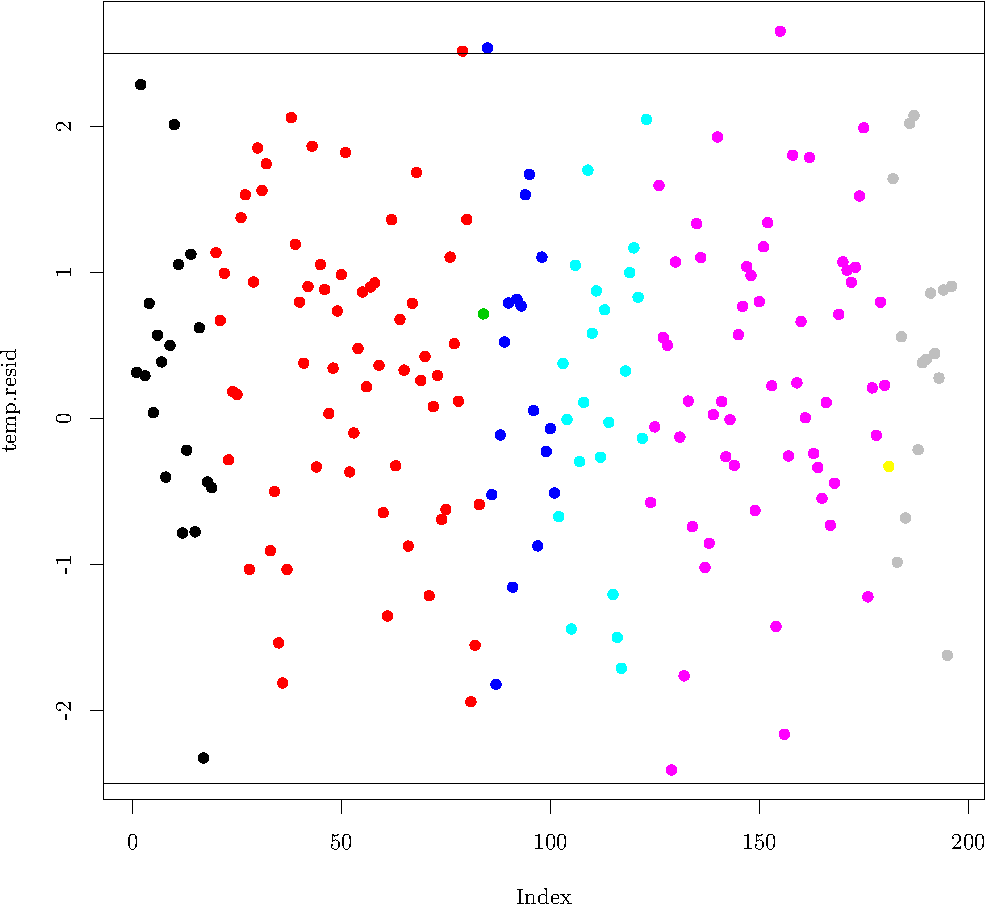
\includegraphics[width=\maxwidth]{figure/05-eda-outliers-full-2} 

}


\begin{kframe}\begin{alltt}
\hlkwd{boxplot}\hlstd{(}\hlkwd{resid}\hlstd{(fit.cph,} \hlkwc{type} \hlstd{=} \hlstr{"deviance"}\hlstd{)} \hlopt{~} \hlstd{data}\hlopt{$}\hlstd{SexM} \hlopt{+} \hlstd{data}\hlopt{$}\hlstd{A2} \hlopt{+} \hlstd{data}\hlopt{$}\hlstd{A4,} \hlkwc{varwidth} \hlstd{=} \hlnum{TRUE}\hlstd{)}
\hlkwd{abline}\hlstd{(}\hlkwc{h} \hlstd{=} \hlnum{0}\hlstd{)}
\end{alltt}
\end{kframe}

{\centering 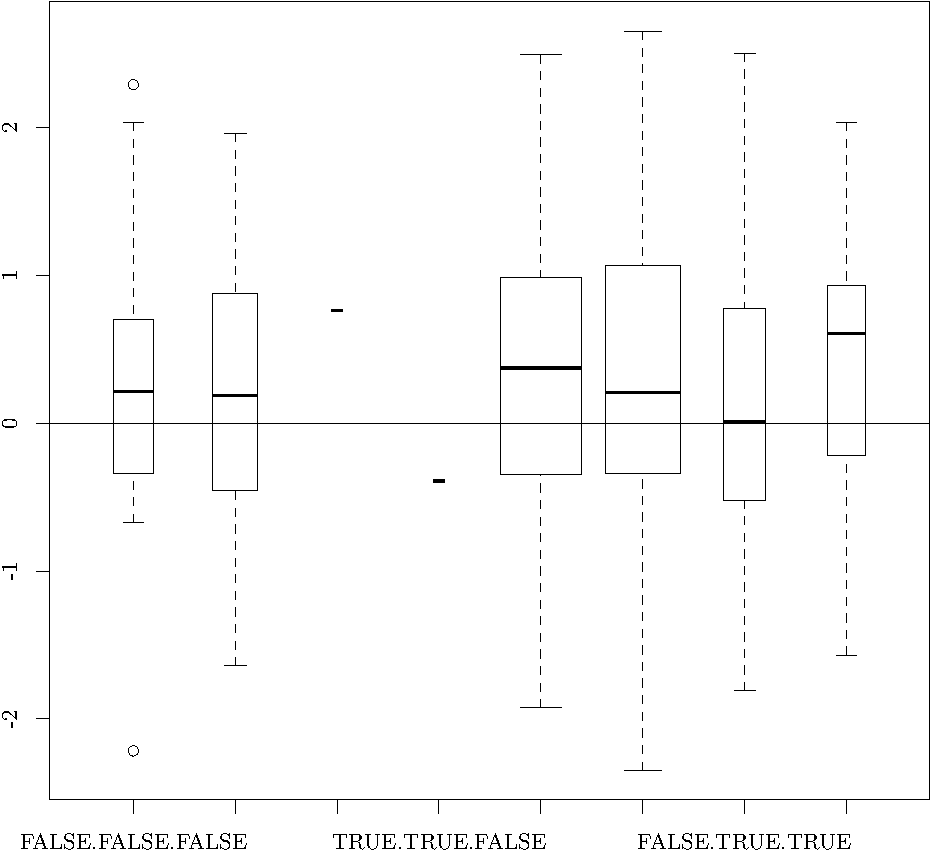
\includegraphics[width=\maxwidth]{figure/05-eda-outliers-full-3} 

}


\begin{kframe}\begin{alltt}
\hlkwd{boxplot}\hlstd{(}\hlkwd{resid}\hlstd{(fit.cph,} \hlkwc{type} \hlstd{=} \hlstr{"martingale"}\hlstd{)} \hlopt{~} \hlstd{data}\hlopt{$}\hlstd{SexM} \hlopt{+} \hlstd{data}\hlopt{$}\hlstd{A2} \hlopt{+} \hlstd{data}\hlopt{$}\hlstd{A4,} \hlkwc{varwidth} \hlstd{=} \hlnum{TRUE}\hlstd{)}
\hlkwd{abline}\hlstd{(}\hlkwc{h} \hlstd{=} \hlnum{0}\hlstd{)}
\end{alltt}
\end{kframe}

{\centering 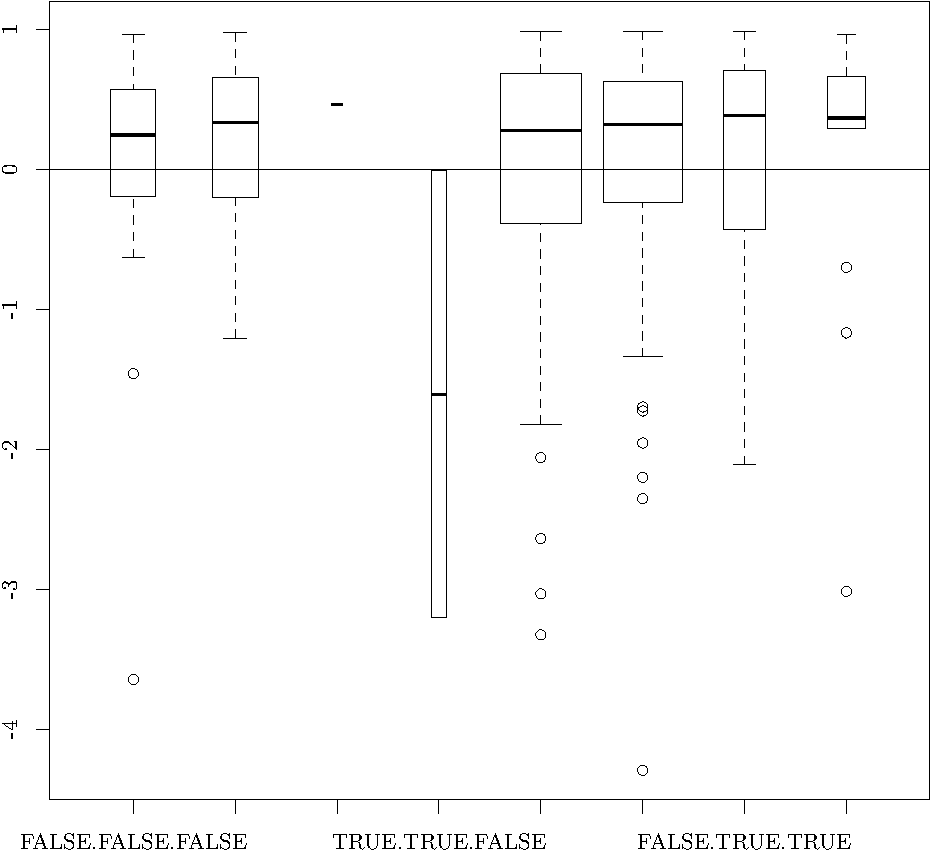
\includegraphics[width=\maxwidth]{figure/05-eda-outliers-full-4} 

}



\end{knitrout}

Use DFBETAS to examine influence.
\begin{knitrout}
\definecolor{shadecolor}{rgb}{0.969, 0.969, 0.969}\color{fgcolor}\begin{kframe}
\begin{alltt}
\hlstd{temp} \hlkwb{=} \hlkwd{resid}\hlstd{(fit.cph,} \hlkwc{type} \hlstd{=} \hlstr{"dfbetas"}\hlstd{)}
\hlkwd{colnames}\hlstd{(temp)} \hlkwb{=} \hlkwd{names}\hlstd{(fit.cph}\hlopt{$}\hlstd{coefficients)}
\hlstd{temp} \hlkwb{=} \hlkwd{melt}\hlstd{(temp)}
\hlkwd{colnames}\hlstd{(temp)} \hlkwb{=} \hlkwd{c}\hlstd{(}\hlstr{"Patient"}\hlstd{,} \hlstr{"Coefficient"}\hlstd{,} \hlstr{"dfbetas"}\hlstd{)}
\hlstd{temp}\hlopt{$}\hlstd{Patient} \hlkwb{=} \hlkwd{gsub}\hlstd{(}\hlstr{"NSWPCN_"}\hlstd{,} \hlstr{""}\hlstd{, temp}\hlopt{$}\hlstd{Patient)}
\hlkwd{ggplot}\hlstd{(temp,} \hlkwd{aes}\hlstd{(}\hlkwc{y} \hlstd{= dfbetas,} \hlkwc{x} \hlstd{= Patient,} \hlkwc{col} \hlstd{= Coefficient))} \hlopt{+} \hlkwd{geom_point}\hlstd{()}
\end{alltt}
\end{kframe}

{\centering 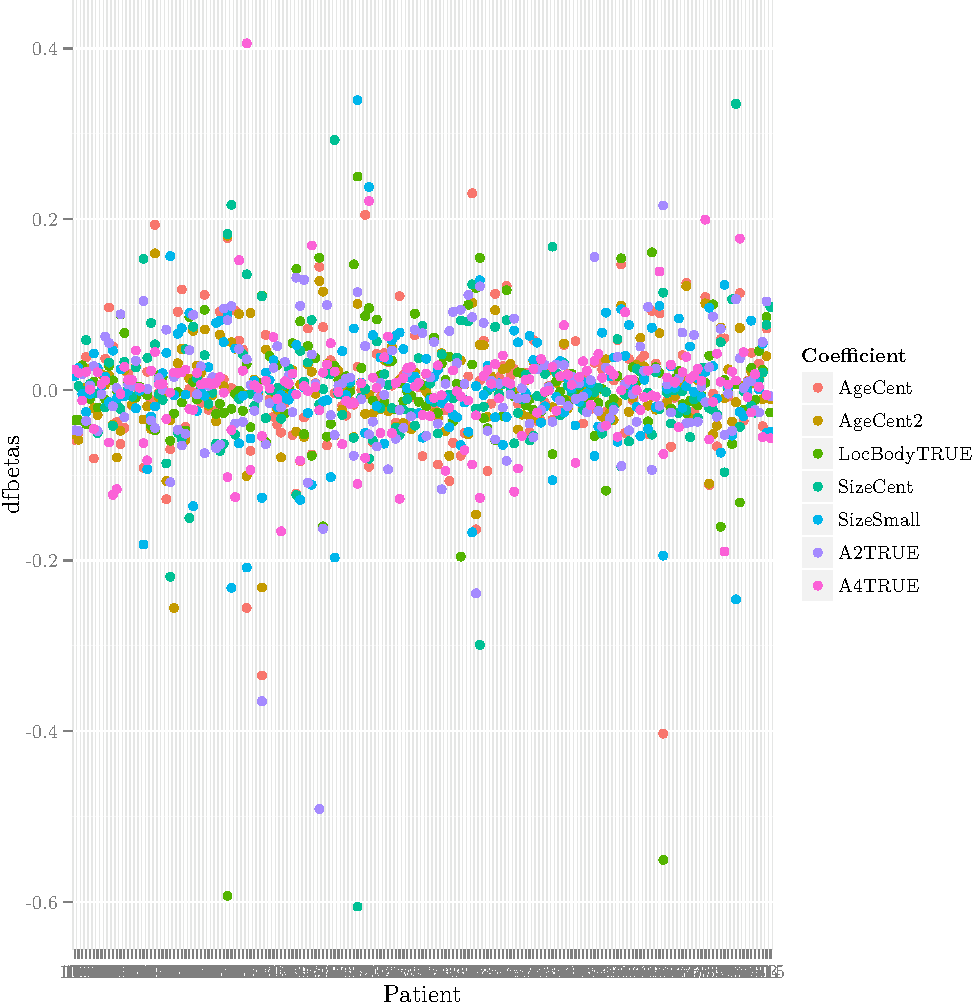
\includegraphics[width=\maxwidth]{figure/05-eda-dfbetas-full-1} 

}



\end{knitrout}
There is quite a number of rather influential observations.  These could do with some checking, but first collapse down the model -- there's little point doing dfbeta fucking about based on coefficients that will never get fit in the end anyway.


\subsection{EDA: Variable selection}
\begin{knitrout}
\definecolor{shadecolor}{rgb}{0.969, 0.969, 0.969}\color{fgcolor}\begin{kframe}
\begin{alltt}
\hlstd{nobs.coxph} \hlkwb{<<-} \hlkwa{function}\hlstd{(}\hlkwc{obj}\hlstd{,} \hlkwc{...}\hlstd{)} \hlkwd{sum}\hlstd{(obj}\hlopt{$}\hlstd{y[,}\hlnum{2}\hlstd{])}
\hlcom{# Note: Exhaustive search at level 2 is only feasible for at most 5 variables}
\hlcom{#fit.cph.as = glmulti(Surv(Time, DSD) ~ strata(SexM) + AgeCent + AgeCent2 + LocBody + SizeCent + SizePlus + A2 + A4, data = data, marginality = TRUE, method = "h", fitfunction = "coxph", crit = "bic", level = 2)}
\hlkwd{set.seed}\hlstd{(}\hlnum{20150110}\hlstd{)}
\hlstd{fit.cph.as} \hlkwb{=} \hlkwd{glmulti}\hlstd{(}\hlkwd{Surv}\hlstd{(Time, DSD)} \hlopt{~} \hlkwd{strata}\hlstd{(SexM)} \hlopt{+} \hlstd{AgeCent} \hlopt{+} \hlstd{AgeCent2} \hlopt{+} \hlstd{LocBody} \hlopt{+} \hlstd{SizeCent} \hlopt{+} \hlstd{SizePlus} \hlopt{+} \hlstd{A2} \hlopt{+} \hlstd{A4,} \hlkwc{data} \hlstd{= data,} \hlkwc{marginality} \hlstd{=} \hlnum{TRUE}\hlstd{,} \hlkwc{method} \hlstd{=} \hlstr{"g"}\hlstd{,} \hlkwc{fitfunction} \hlstd{=} \hlstr{"coxph"}\hlstd{,} \hlkwc{crit} \hlstd{=} \hlstr{"bic"}\hlstd{,} \hlkwc{level} \hlstd{=} \hlnum{2}\hlstd{,} \hlkwc{plotty} \hlstd{=} \hlnum{FALSE}\hlstd{,} \hlkwc{report} \hlstd{=} \hlnum{TRUE}\hlstd{)}
\end{alltt}
\begin{verbatim}
## Initialization...
## TASK: Genetic algorithm in the candidate set.
## Initialization...
## Algorithm started...
## 
## After 10 generations:
## Best model: Surv(Time,DSD)~1+strata(SexM)+AgeCent2+LocBody+SizeCent+SizePlus+A2+A4+SizePlus:SizeCent+A2:AgeCent2+A2:LocBody+A2:SizeCent+A4:AgeCent2+A4:LocBody+A4:A2
## Crit= 1354.28574554096
## Mean crit= 1389.08061331627
## Change in best IC: -8645.71425445904 / Change in mean IC: -8610.91938668373
## 
## After 20 generations:
## Best model: Surv(Time,DSD)~1+strata(SexM)+AgeCent2+LocBody+SizeCent+SizePlus+A2+A4+SizePlus:AgeCent2+A2:AgeCent2+A2:LocBody+A2:SizeCent+A2:SizePlus+A4:SizeCent
## Crit= 1347.5197391119
## Mean crit= 1380.49806590263
## Change in best IC: -6.76600642905873 / Change in mean IC: -8.5825474136393
## 
## After 30 generations:
## Best model: Surv(Time,DSD)~1+strata(SexM)+AgeCent2+SizeCent+SizePlus+A2+A4+A2:AgeCent2+A2:SizeCent+A2:SizePlus+A4:SizeCent
## Crit= 1335.47630295753
## Mean crit= 1377.01558685262
## Change in best IC: -12.0434361543705 / Change in mean IC: -3.48247905001313
## 
## After 40 generations:
## Best model: Surv(Time,DSD)~1+strata(SexM)+AgeCent2+SizeCent+SizePlus+A2+A4+A2:AgeCent2+A2:SizeCent+A2:SizePlus+A4:SizeCent
## Crit= 1335.47630295753
## Mean crit= 1373.6984486489
## Change in best IC: 0 / Change in mean IC: -3.3171382037242
## 
## After 50 generations:
## Best model: Surv(Time,DSD)~1+strata(SexM)+AgeCent2+SizeCent+SizePlus+A2+A4+A2:SizeCent+A2:SizePlus
## Crit= 1327.30049854276
## Mean crit= 1370.31952603325
## Change in best IC: -8.1758044147673 / Change in mean IC: -3.37892261564252
## 
## After 60 generations:
## Best model: Surv(Time,DSD)~1+strata(SexM)+AgeCent2+SizeCent+SizePlus+A2+A4+A2:SizeCent+A2:SizePlus+A4:A2
## Crit= 1327.05884451455
## Mean crit= 1368.52203696429
## Change in best IC: -0.241654028217681 / Change in mean IC: -1.79748906896225
## 
## After 70 generations:
## Best model: Surv(Time,DSD)~1+strata(SexM)+SizeCent+SizePlus+A2+A4+A2:SizeCent+A2:SizePlus+A4:A2
## Crit= 1322.2188775423
## Mean crit= 1367.33736017854
## Change in best IC: -4.83996697225052 / Change in mean IC: -1.18467678575053
## 
## After 80 generations:
## Best model: Surv(Time,DSD)~1+strata(SexM)+SizeCent+SizePlus+A2+A4+A2:SizeCent+A2:SizePlus+A4:A2
## Crit= 1322.2188775423
## Mean crit= 1364.87343806893
## Change in best IC: 0 / Change in mean IC: -2.46392210960857
## 
## After 90 generations:
## Best model: Surv(Time,DSD)~1+strata(SexM)+SizeCent+SizePlus+A2+A4+A2:SizeCent+A2:SizePlus
## Crit= 1322.1189070341
## Mean crit= 1363.4646098969
## Change in best IC: -0.0999705081956108 / Change in mean IC: -1.40882817202873
## 
## After 100 generations:
## Best model: Surv(Time,DSD)~1+strata(SexM)+SizeCent+SizePlus+A2+A4+A2:SizeCent+A2:SizePlus
## Crit= 1322.1189070341
## Mean crit= 1362.68636612614
## Change in best IC: 0 / Change in mean IC: -0.77824377076422
## 
## After 110 generations:
## Best model: Surv(Time,DSD)~1+strata(SexM)+SizeCent+SizePlus+A2+A4+A2:SizeCent+A2:SizePlus
## Crit= 1322.1189070341
## Mean crit= 1361.22836551388
## Change in best IC: 0 / Change in mean IC: -1.45800061225532
## 
## After 120 generations:
## Best model: Surv(Time,DSD)~1+strata(SexM)+SizeCent+SizePlus+A2+A4+A2:SizeCent+A2:SizePlus
## Crit= 1322.1189070341
## Mean crit= 1359.50645469942
## Change in best IC: 0 / Change in mean IC: -1.7219108144634
## 
## After 130 generations:
## Best model: Surv(Time,DSD)~1+strata(SexM)+SizeCent+SizePlus+A2+A4+A2:SizeCent+A2:SizePlus
## Crit= 1322.1189070341
## Mean crit= 1358.59551250947
## Change in best IC: 0 / Change in mean IC: -0.910942189947946
## 
## After 140 generations:
## Best model: Surv(Time,DSD)~1+strata(SexM)+SizeCent+SizePlus+A2+A4+A2:SizeCent+A2:SizePlus
## Crit= 1322.1189070341
## Mean crit= 1358.01538857016
## Change in best IC: 0 / Change in mean IC: -0.580123939309942
## 
## After 150 generations:
## Best model: Surv(Time,DSD)~1+strata(SexM)+SizeCent+SizePlus+A2+A4+A2:SizeCent+A2:SizePlus
## Crit= 1322.1189070341
## Mean crit= 1357.9376161506
## Change in best IC: 0 / Change in mean IC: -0.0777724195659175
## 
## After 160 generations:
## Best model: Surv(Time,DSD)~1+strata(SexM)+SizeCent+SizePlus+A2+A4+A2:SizeCent+A2:SizePlus
## Crit= 1322.1189070341
## Mean crit= 1356.46885834002
## Change in best IC: 0 / Change in mean IC: -1.46875781057724
## 
## After 170 generations:
## Best model: Surv(Time,DSD)~1+strata(SexM)+SizeCent+SizePlus+A2+A4+A2:SizeCent+A2:SizePlus
## Crit= 1322.1189070341
## Mean crit= 1355.4352368695
## Change in best IC: 0 / Change in mean IC: -1.03362147052326
## 
## After 180 generations:
## Best model: Surv(Time,DSD)~1+strata(SexM)+SizeCent+SizePlus+A2+A4+A2:SizeCent+A2:SizePlus
## Crit= 1322.1189070341
## Mean crit= 1355.4352368695
## Change in best IC: 0 / Change in mean IC: 0
\end{verbatim}


{\ttfamily\noindent\color{warningcolor}{\#\# Warning in fitter(X, Y, strats, offset, init, control, weights = weights, : Loglik converged before variable\ \ 3 ; beta may be infinite.}}\begin{verbatim}
## 
## After 190 generations:
## Best model: Surv(Time,DSD)~1+strata(SexM)+SizeCent+A2+A4+A2:SizeCent
## Crit= 1319.04026884741
## Mean crit= 1354.42684856463
## Change in best IC: -3.0786381866892 / Change in mean IC: -1.00838830486259
## 
## After 200 generations:
## Best model: Surv(Time,DSD)~1+strata(SexM)+SizeCent+A2+A4+A2:SizeCent
## Crit= 1319.04026884741
## Mean crit= 1354.2616269749
## Change in best IC: 0 / Change in mean IC: -0.165221589737939
## 
## After 210 generations:
## Best model: Surv(Time,DSD)~1+strata(SexM)+SizeCent+A2+A4
## Crit= 1313.86182415827
## Mean crit= 1352.48919986557
## Change in best IC: -5.17844468913768 / Change in mean IC: -1.7724271093266
## 
## After 220 generations:
## Best model: Surv(Time,DSD)~1+strata(SexM)+SizeCent+A2+A4
## Crit= 1313.86182415827
## Mean crit= 1351.81721667487
## Change in best IC: 0 / Change in mean IC: -0.671983190697119
\end{verbatim}


{\ttfamily\noindent\color{warningcolor}{\#\# Warning in fitter(X, Y, strats, offset, init, control, weights = weights, : Loglik converged before variable\ \ 3 ; beta may be infinite.}}\begin{verbatim}
## 
## After 230 generations:
## Best model: Surv(Time,DSD)~1+strata(SexM)+SizeCent+A2+A4
## Crit= 1313.86182415827
## Mean crit= 1350.98166979759
## Change in best IC: 0 / Change in mean IC: -0.835546877286561
## 
## After 240 generations:
## Best model: Surv(Time,DSD)~1+strata(SexM)+SizeCent+A2+A4
## Crit= 1313.86182415827
## Mean crit= 1350.72264968577
## Change in best IC: 0 / Change in mean IC: -0.259020111812561
## 
## After 250 generations:
## Best model: Surv(Time,DSD)~1+strata(SexM)+SizeCent+A2+A4
## Crit= 1313.86182415827
## Mean crit= 1350.72264968577
## Change in best IC: 0 / Change in mean IC: 0
## 
## After 260 generations:
## Best model: Surv(Time,DSD)~1+strata(SexM)+SizeCent+A2+A4
## Crit= 1313.86182415827
## Mean crit= 1349.09919154119
## Change in best IC: 0 / Change in mean IC: -1.62345814458763
## 
## After 270 generations:
## Best model: Surv(Time,DSD)~1+strata(SexM)+SizeCent+A2+A4
## Crit= 1313.86182415827
## Mean crit= 1348.97499717855
## Change in best IC: 0 / Change in mean IC: -0.124194362634853
## 
## After 280 generations:
## Best model: Surv(Time,DSD)~1+strata(SexM)+SizeCent+A2+A4
## Crit= 1313.86182415827
## Mean crit= 1348.20047884048
## Change in best IC: 0 / Change in mean IC: -0.774518338069356
## 
## After 290 generations:
## Best model: Surv(Time,DSD)~1+strata(SexM)+SizeCent+A2+A4
## Crit= 1313.86182415827
## Mean crit= 1347.63434266772
## Change in best IC: 0 / Change in mean IC: -0.566136172765709
## 
## After 300 generations:
## Best model: Surv(Time,DSD)~1+strata(SexM)+SizeCent+A2+A4
## Crit= 1313.86182415827
## Mean crit= 1347.63434266772
## Change in best IC: 0 / Change in mean IC: 0
## 
## After 310 generations:
## Best model: Surv(Time,DSD)~1+strata(SexM)+SizeCent+A2+A4
## Crit= 1313.86182415827
## Mean crit= 1347.63434266772
## Change in best IC: 0 / Change in mean IC: 0
## 
## After 320 generations:
## Best model: Surv(Time,DSD)~1+strata(SexM)+SizeCent+A2+A4
## Crit= 1313.86182415827
## Mean crit= 1347.50385351425
## Change in best IC: 0 / Change in mean IC: -0.130489153465305
## 
## After 330 generations:
## Best model: Surv(Time,DSD)~1+strata(SexM)+SizeCent+A2+A4
## Crit= 1313.86182415827
## Mean crit= 1347.50385351425
## Change in best IC: 0 / Change in mean IC: 0
## 
## After 340 generations:
## Best model: Surv(Time,DSD)~1+strata(SexM)+SizeCent+A2+A4
## Crit= 1313.86182415827
## Mean crit= 1347.46832064224
## Change in best IC: 0 / Change in mean IC: -0.0355328720097532
## 
## After 350 generations:
## Best model: Surv(Time,DSD)~1+strata(SexM)+SizeCent+A2+A4
## Crit= 1313.86182415827
## Mean crit= 1346.2647364989
## Change in best IC: 0 / Change in mean IC: -1.20358414334032
## 
## After 360 generations:
## Best model: Surv(Time,DSD)~1+strata(SexM)+SizeCent+A2+A4
## Crit= 1313.86182415827
## Mean crit= 1346.23872029283
## Change in best IC: 0 / Change in mean IC: -0.0260162060701532
## 
## After 370 generations:
## Best model: Surv(Time,DSD)~1+strata(SexM)+SizeCent+A2+A4
## Crit= 1313.86182415827
## Mean crit= 1346.10925658884
## Change in best IC: 0 / Change in mean IC: -0.129463703985721
## 
## After 380 generations:
## Best model: Surv(Time,DSD)~1+strata(SexM)+SizeCent+A2+A4
## Crit= 1313.86182415827
## Mean crit= 1345.53002602703
## Change in best IC: 0 / Change in mean IC: -0.579230561817212
## 
## After 390 generations:
## Best model: Surv(Time,DSD)~1+strata(SexM)+SizeCent+A2+A4
## Crit= 1313.86182415827
## Mean crit= 1345.53002602703
## Change in best IC: 0 / Change in mean IC: 0
## 
## After 400 generations:
## Best model: Surv(Time,DSD)~1+strata(SexM)+SizeCent+A2+A4
## Crit= 1313.86182415827
## Mean crit= 1345.5077951485
## Change in best IC: 0 / Change in mean IC: -0.0222308785255336
## 
## After 410 generations:
## Best model: Surv(Time,DSD)~1+strata(SexM)+SizeCent+A2+A4
## Crit= 1313.86182415827
## Mean crit= 1345.50206758174
## Change in best IC: 0 / Change in mean IC: -0.00572756675614983
## 
## After 420 generations:
## Best model: Surv(Time,DSD)~1+strata(SexM)+SizeCent+A2+A4
## Crit= 1313.86182415827
## Mean crit= 1345.20503158788
## Change in best IC: 0 / Change in mean IC: -0.297035993865393
## 
## After 430 generations:
## Best model: Surv(Time,DSD)~1+strata(SexM)+SizeCent+A2+A4
## Crit= 1313.86182415827
## Mean crit= 1345.06006511155
## Change in best IC: 0 / Change in mean IC: -0.144966476329046
## 
## After 440 generations:
## Best model: Surv(Time,DSD)~1+strata(SexM)+SizeCent+A2+A4
## Crit= 1313.86182415827
## Mean crit= 1344.91463821575
## Change in best IC: 0 / Change in mean IC: -0.145426895802984
## 
## After 450 generations:
## Best model: Surv(Time,DSD)~1+strata(SexM)+SizeCent+A2+A4
## Crit= 1313.86182415827
## Mean crit= 1344.27812042665
## Change in best IC: 0 / Change in mean IC: -0.636517789095478
## 
## After 460 generations:
## Best model: Surv(Time,DSD)~1+strata(SexM)+SizeCent+A2+A4
## Crit= 1313.86182415827
## Mean crit= 1344.2388364852
## Change in best IC: 0 / Change in mean IC: -0.0392839414539594
## 
## After 470 generations:
## Best model: Surv(Time,DSD)~1+strata(SexM)+SizeCent+A2+A4
## Crit= 1313.86182415827
## Mean crit= 1344.2388364852
## Change in best IC: 0 / Change in mean IC: 0
## 
## After 480 generations:
## Best model: Surv(Time,DSD)~1+strata(SexM)+SizeCent+A2+A4
## Crit= 1313.86182415827
## Mean crit= 1344.21229867826
## Change in best IC: 0 / Change in mean IC: -0.0265378069345843
## 
## After 490 generations:
## Best model: Surv(Time,DSD)~1+strata(SexM)+SizeCent+A2+A4
## Crit= 1313.86182415827
## Mean crit= 1344.19890365158
## Change in best IC: 0 / Change in mean IC: -0.013395026684293
## 
## After 500 generations:
## Best model: Surv(Time,DSD)~1+strata(SexM)+SizeCent+A2+A4
## Crit= 1313.86182415827
## Mean crit= 1344.19042753282
## Improvements in best and average IC have bebingo en below the specified goals.
## Algorithm is declared to have converged.
## Completed.
\end{verbatim}
\begin{alltt}
\hlcom{# fit.cph.as}
\hlcom{# After 830 generations:}
\hlcom{# Best model: Surv(Time,DSD)~1+strata(SexM)+SizeCent+A2+A4}
\hlcom{# Crit= 1367.16344569113}
\hlcom{# Mean crit= 1401.37248769175}
\hlcom{# Improvements in best and average IC have bebingo en below the specified goals.}
\hlcom{# Algorithm is declared to have converged.}
\hlcom{# Completed.}
\hlstd{fit.cph.as}
\end{alltt}
\begin{verbatim}
## An object of class "glmulti"
## Slot "name":
## [1] "glmulti.analysis"
## 
## Slot "params":
## $name
## [1] "glmulti.analysis"
## 
## $intercept
## [1] TRUE
## 
## $marginality
## [1] TRUE
## 
## $bnch
## [1] 30
## 
## $chunk
## [1] 1
## 
## $chunks
## [1] 1
## 
## $level
## [1] 2
## 
## $minsize
## [1] 0
## 
## $maxsize
## [1] -1
## 
## $minK
## [1] 0
## 
## $maxK
## [1] -1
## 
## $method
## [1] "g"
## 
## $crit
## [1] "bic"
## 
## $confsetsize
## [1] 100
## 
## $fitfunction
## [1] "coxph"
## 
## $popsize
## [1] 100
## 
## $mutrate
## [1] 0.001
## 
## $sexrate
## [1] 0.1
## 
## $imm
## [1] 0.3
## 
## $plotty
## [1] FALSE
## 
## $deltaM
## [1] 0.05
## 
## $deltaB
## [1] 0.05
## 
## $conseq
## [1] 5
## 
## $resumefile
## [1] "id"
## 
## $generations
## [1] 500
## 
## $elapsed
## [1] 4.159
## 
## $dynat
##  [1]  6.001 10.904 15.749 20.504 25.417 30.367 34.698 39.977 44.896 50.288
## [11] 54.940  1.007  1.092  1.175  1.258  1.330  1.408  1.496  1.576  1.657
## [21]  1.740  1.823  1.900  1.978  2.058  2.139  2.234  2.309  2.385  2.459
## [31]  2.538  2.620  2.698  2.801  2.884  2.968  3.050  3.143  3.227  3.306
## [41]  3.384  3.463  3.540  3.614  3.707  3.787  3.882  3.978  4.059  4.139
## 
## $dynab
##  [1] 1354 1348 1335 1335 1327 1327 1322 1322 1322 1322 1322 1322 1322 1322
## [15] 1322 1322 1322 1322 1319 1319 1314 1314 1314 1314 1314 1314 1314 1314
## [29] 1314 1314 1314 1314 1314 1314 1314 1314 1314 1314 1314 1314 1314 1314
## [43] 1314 1314 1314 1314 1314 1314 1314 1314
## 
## $dynam
##  [1] 1389 1380 1377 1374 1370 1369 1367 1365 1363 1363 1361 1360 1359 1358
## [15] 1358 1356 1355 1355 1354 1354 1352 1352 1351 1351 1351 1349 1349 1348
## [29] 1348 1348 1348 1348 1348 1347 1346 1346 1346 1346 1346 1346 1346 1345
## [43] 1345 1345 1344 1344 1344 1344 1344 1344
## 
## 
## Slot "nbmods":
## [1] 100
## 
## Slot "crits":
##   [1] 1314 1315 1316 1316 1316 1317 1318 1318 1318 1318 1318 1319 1319 1319
##  [15] 1322 1322 1323 1323 1323 1323 1323 1325 1325 1325 1326 1326 1327 1327
##  [29] 1327 1327 1327 1327 1327 1327 1328 1329 1335 1338 1339 1341 1341 1341
##  [43] 1348 1348 1349 1350 1351 1351 1353 1353 1353 1354 1354 1354 1354 1354
##  [57] 1355 1355 1355 1356 1357 1357 1357 1357 1357 1358 1358 1358 1359 1359
##  [71] 1359 1359 1359 1360 1360 1360 1361 1361 1361 1361 1362 1362 1362 1362
##  [85] 1362 1363 1363 1363 1363 1363 1363 1363 1363 1363 1363 1364 1364 1364
##  [99] 1364 1364
## 
## Slot "K":
##   [1]  4  3  3  5  3  5  5  5  5  5  5  5  5  5  7  8  6  6  6  6  6  8  8
##  [24]  7  8  9  8  8  9  9  8  8  9  7  7  9 10 11 11 11 11 11 13 14 12 11
##  [47] 14 15 12 14 13 14 15 14 14 13 13 14 14 14 13 15 15 14 14 14 16 15 17
##  [70] 15 15 16 15 16 15 17 16 15 15 17 15 15 15 15 16 16 15 16 16 15 16 16
##  [93] 15 17 16 17 15 15 17 15
## 
## Slot "formulas":
## [[1]]
## Surv(Time, DSD) ~ 1 + strata(SexM) + SizeCent + A2 + A4
## <environment: 0x5313260>
## 
## [[2]]
## Surv(Time, DSD) ~ 1 + strata(SexM) + A2 + A4
## <environment: 0x5313260>
## 
## [[3]]
## Surv(Time, DSD) ~ 1 + strata(SexM) + SizeCent + A2
## <environment: 0x5313260>
## 
## [[4]]
## Surv(Time, DSD) ~ 1 + strata(SexM) + SizeCent + A2 + A4 + A4:A2
## <environment: 0x5313260>
## 
## [[5]]
## Surv(Time, DSD) ~ 1 + strata(SexM) + SizeCent + A4
## <environment: 0x5313260>
## 
## [[6]]
## Surv(Time, DSD) ~ 1 + strata(SexM) + SizeCent + A2 + A4 + strata(SexM):SizeCent
## <environment: 0x5313260>
## 
## [[7]]
## Surv(Time, DSD) ~ 1 + strata(SexM) + SizeCent + A2 + A4 + A4:SizeCent
## <environment: 0x5313260>
## 
## [[8]]
## Surv(Time, DSD) ~ 1 + strata(SexM) + LocBody + SizeCent + A2 + 
##     A4
## <environment: 0x5313260>
## 
## [[9]]
## Surv(Time, DSD) ~ 1 + strata(SexM) + SizeCent + SizePlus + A2 + 
##     A4
## <environment: 0x5313260>
## 
## [[10]]
## Surv(Time, DSD) ~ 1 + strata(SexM) + SizeCent + A2 + A4 + strata(SexM):A2
## <environment: 0x5313260>
## 
## [[11]]
## Surv(Time, DSD) ~ 1 + strata(SexM) + AgeCent + SizeCent + A2 + 
##     A4
## <environment: 0x5313260>
## 
## [[12]]
## Surv(Time, DSD) ~ 1 + strata(SexM) + AgeCent2 + SizeCent + A2 + 
##     A4
## <environment: 0x5313260>
## 
## [[13]]
## Surv(Time, DSD) ~ 1 + strata(SexM) + SizeCent + A2 + A4 + strata(SexM):A4
## <environment: 0x5313260>
## 
## [[14]]
## Surv(Time, DSD) ~ 1 + strata(SexM) + SizeCent + A2 + A4 + A2:SizeCent
## <environment: 0x5313260>
## 
## [[15]]
## Surv(Time, DSD) ~ 1 + strata(SexM) + SizeCent + SizePlus + A2 + 
##     A4 + A2:SizeCent + A2:SizePlus
## <environment: 0x5313260>
## 
## [[16]]
## Surv(Time, DSD) ~ 1 + strata(SexM) + SizeCent + SizePlus + A2 + 
##     A4 + A2:SizeCent + A2:SizePlus + A4:A2
## <environment: 0x5313260>
## 
## [[17]]
## Surv(Time, DSD) ~ 1 + strata(SexM) + SizeCent + SizePlus + A2 + 
##     A4 + A2:SizePlus
## <environment: 0x5313260>
## 
## [[18]]
## Surv(Time, DSD) ~ 1 + strata(SexM) + AgeCent + LocBody + SizeCent + 
##     A2 + A4
## <environment: 0x5313260>
## 
## [[19]]
## Surv(Time, DSD) ~ 1 + strata(SexM) + SizeCent + SizePlus + A2 + 
##     A2:SizeCent + A2:SizePlus
## <environment: 0x5313260>
## 
## [[20]]
## Surv(Time, DSD) ~ 1 + strata(SexM) + LocBody + SizeCent + A2 + 
##     A4 + A2:SizeCent
## <environment: 0x5313260>
## 
## [[21]]
## Surv(Time, DSD) ~ 1 + strata(SexM) + SizeCent + SizePlus + A2 + 
##     A4 + A2:SizeCent
## <environment: 0x5313260>
## 
## [[22]]
## Surv(Time, DSD) ~ 1 + strata(SexM) + SizeCent + SizePlus + A2 + 
##     A4 + A2:SizeCent + A2:SizePlus + strata(SexM):SizePlus
## <environment: 0x5313260>
## 
## [[23]]
## Surv(Time, DSD) ~ 1 + strata(SexM) + SizeCent + SizePlus + A2 + 
##     A4 + A2:SizeCent + A2:SizePlus + strata(SexM):SizeCent
## <environment: 0x5313260>
## 
## [[24]]
## Surv(Time, DSD) ~ 1 + strata(SexM) + SizeCent + SizePlus + A2 + 
##     A4 + A2:SizeCent + A4:A2
## <environment: 0x5313260>
## 
## [[25]]
## Surv(Time, DSD) ~ 1 + strata(SexM) + LocBody + SizeCent + SizePlus + 
##     A2 + A4 + A2:SizeCent + A2:SizePlus
## <environment: 0x5313260>
## 
## [[26]]
## Surv(Time, DSD) ~ 1 + strata(SexM) + SizeCent + SizePlus + A2 + 
##     A4 + A2:SizeCent + A2:SizePlus + A4:SizeCent + A4:A2
## <environment: 0x5313260>
## 
## [[27]]
## Surv(Time, DSD) ~ 1 + strata(SexM) + SizeCent + SizePlus + A2 + 
##     A4 + A2:SizeCent + A2:SizePlus + A4:SizeCent
## <environment: 0x5313260>
## 
## [[28]]
## Surv(Time, DSD) ~ 1 + strata(SexM) + SizeCent + SizePlus + A2 + 
##     A4 + A2:SizeCent + A2:SizePlus + A4:SizePlus
## <environment: 0x5313260>
## 
## [[29]]
## Surv(Time, DSD) ~ 1 + strata(SexM) + AgeCent2 + SizeCent + SizePlus + 
##     A2 + A4 + A2:SizeCent + A2:SizePlus + A4:A2
## <environment: 0x5313260>
## 
## [[30]]
## Surv(Time, DSD) ~ 1 + strata(SexM) + SizeCent + SizePlus + A2 + 
##     A4 + SizePlus:SizeCent + A2:SizeCent + A2:SizePlus + A4:A2
## <environment: 0x5313260>
## 
## [[31]]
## Surv(Time, DSD) ~ 1 + strata(SexM) + SizeCent + SizePlus + A2 + 
##     A4 + A2:SizeCent + A2:SizePlus + strata(SexM):A4
## <environment: 0x5313260>
## 
## [[32]]
## Surv(Time, DSD) ~ 1 + strata(SexM) + AgeCent2 + SizeCent + SizePlus + 
##     A2 + A4 + A2:SizeCent + A2:SizePlus
## <environment: 0x5313260>
## 
## [[33]]
## Surv(Time, DSD) ~ 1 + strata(SexM) + SizeCent + SizePlus + A2 + 
##     A4 + A2:SizeCent + A2:SizePlus + A4:A2 + strata(SexM):A2
## <environment: 0x5313260>
## 
## [[34]]
## Surv(Time, DSD) ~ 1 + strata(SexM) + AgeCent2 + SizeCent + SizePlus + 
##     A2 + A4 + A2:SizePlus
## <environment: 0x5313260>
## 
## [[35]]
## Surv(Time, DSD) ~ 1 + strata(SexM) + AgeCent2 + SizeCent + SizePlus + 
##     A2 + A4 + A2:SizeCent
## <environment: 0x5313260>
## 
## [[36]]
## Surv(Time, DSD) ~ 1 + strata(SexM) + AgeCent2 + SizeCent + SizePlus + 
##     A2 + A4 + SizeCent:AgeCent2 + A2:SizeCent + A2:SizePlus
## <environment: 0x5313260>
## 
## [[37]]
## Surv(Time, DSD) ~ 1 + strata(SexM) + AgeCent2 + SizeCent + SizePlus + 
##     A2 + A4 + A2:AgeCent2 + A2:SizeCent + A2:SizePlus + A4:SizeCent
## <environment: 0x5313260>
## 
## [[38]]
## Surv(Time, DSD) ~ 1 + strata(SexM) + AgeCent2 + SizeCent + SizePlus + 
##     A2 + A4 + SizeCent:AgeCent2 + A2:AgeCent2 + A2:SizeCent + 
##     A2:SizePlus + A4:SizeCent
## <environment: 0x5313260>
## 
## [[39]]
## Surv(Time, DSD) ~ 1 + strata(SexM) + AgeCent2 + LocBody + SizeCent + 
##     SizePlus + A2 + A4 + A2:AgeCent2 + A2:SizeCent + A2:SizePlus + 
##     A4:SizeCent
## <environment: 0x5313260>
## 
## [[40]]
## Surv(Time, DSD) ~ 1 + strata(SexM) + AgeCent2 + SizeCent + SizePlus + 
##     A2 + A4 + A2:AgeCent2 + A2:SizeCent + A2:SizePlus + A4:SizeCent + 
##     strata(SexM):AgeCent2
## <environment: 0x5313260>
## 
## [[41]]
## Surv(Time, DSD) ~ 1 + strata(SexM) + AgeCent2 + SizeCent + SizePlus + 
##     A2 + A4 + A2:AgeCent2 + A2:SizeCent + A2:SizePlus + A4:SizeCent + 
##     strata(SexM):A4
## <environment: 0x5313260>
## 
## [[42]]
## Surv(Time, DSD) ~ 1 + strata(SexM) + AgeCent2 + SizeCent + SizePlus + 
##     A2 + A4 + A2:AgeCent2 + A2:SizeCent + A2:SizePlus + A4:SizeCent + 
##     A4:SizePlus
## <environment: 0x5313260>
## 
## [[43]]
## Surv(Time, DSD) ~ 1 + strata(SexM) + AgeCent2 + LocBody + SizeCent + 
##     SizePlus + A2 + A4 + SizePlus:AgeCent2 + A2:AgeCent2 + A2:LocBody + 
##     A2:SizeCent + A2:SizePlus + A4:SizeCent
## <environment: 0x5313260>
## 
## [[44]]
## Surv(Time, DSD) ~ 1 + strata(SexM) + AgeCent2 + LocBody + SizeCent + 
##     SizePlus + A2 + A4 + SizeCent:AgeCent2 + SizeCent:LocBody + 
##     A2:LocBody + A2:SizeCent + A2:SizePlus + A4:SizeCent + A4:A2
## <environment: 0x5313260>
## 
## [[45]]
## Surv(Time, DSD) ~ 1 + strata(SexM) + LocBody + SizeCent + SizePlus + 
##     A2 + A4 + A2:LocBody + A4:LocBody + A4:SizeCent + A4:SizePlus + 
##     strata(SexM):LocBody + strata(SexM):SizeCent
## <environment: 0x5313260>
## 
## [[46]]
## Surv(Time, DSD) ~ 1 + strata(SexM) + AgeCent + AgeCent2 + SizeCent + 
##     SizePlus + A4 + SizePlus:AgeCent2 + SizePlus:SizeCent + A4:AgeCent + 
##     A4:SizeCent + strata(SexM):SizeCent
## <environment: 0x5313260>
## 
## [[47]]
## Surv(Time, DSD) ~ 1 + strata(SexM) + AgeCent + AgeCent2 + LocBody + 
##     SizeCent + SizePlus + A2 + A4 + AgeCent2:AgeCent + SizeCent:AgeCent2 + 
##     A4:AgeCent2 + A4:SizePlus + A4:A2 + strata(SexM):A2
## <environment: 0x5313260>
## 
## [[48]]
## Surv(Time, DSD) ~ 1 + strata(SexM) + AgeCent + LocBody + SizeCent + 
##     SizePlus + A2 + A4 + SizePlus:AgeCent + A2:LocBody + A2:SizeCent + 
##     A2:SizePlus + A4:SizePlus + A4:A2 + strata(SexM):SizePlus + 
##     strata(SexM):A4
## <environment: 0x5313260>
## 
## [[49]]
## Surv(Time, DSD) ~ 1 + strata(SexM) + AgeCent + AgeCent2 + LocBody + 
##     SizeCent + SizePlus + A4 + SizePlus:SizeCent + A4:AgeCent2 + 
##     A4:SizePlus + strata(SexM):AgeCent + strata(SexM):LocBody
## <environment: 0x5313260>
## 
## [[50]]
## Surv(Time, DSD) ~ 1 + strata(SexM) + AgeCent2 + LocBody + SizeCent + 
##     SizePlus + A2 + A4 + SizePlus:AgeCent2 + A2:AgeCent2 + A2:LocBody + 
##     A2:SizeCent + A2:SizePlus + A4:SizeCent + strata(SexM):LocBody
## <environment: 0x5313260>
## 
## [[51]]
## Surv(Time, DSD) ~ 1 + strata(SexM) + AgeCent + AgeCent2 + LocBody + 
##     SizeCent + SizePlus + A2 + A4 + LocBody:AgeCent2 + SizeCent:AgeCent + 
##     SizePlus:AgeCent + A2:SizeCent + A4:AgeCent
## <environment: 0x5313260>
## 
## [[52]]
## Surv(Time, DSD) ~ 1 + strata(SexM) + AgeCent2 + LocBody + SizeCent + 
##     SizePlus + A2 + A4 + SizePlus:AgeCent2 + A2:AgeCent2 + A2:LocBody + 
##     A2:SizeCent + A4:AgeCent2 + A4:LocBody + A4:A2
## <environment: 0x5313260>
## 
## [[53]]
## Surv(Time, DSD) ~ 1 + strata(SexM) + AgeCent + AgeCent2 + LocBody + 
##     SizeCent + SizePlus + A2 + A4 + SizePlus:AgeCent2 + A2:AgeCent + 
##     A2:SizeCent + A2:SizePlus + A4:A2 + strata(SexM):AgeCent2 + 
##     strata(SexM):LocBody
## <environment: 0x5313260>
## 
## [[54]]
## Surv(Time, DSD) ~ 1 + strata(SexM) + AgeCent2 + LocBody + SizeCent + 
##     SizePlus + A2 + A4 + SizePlus:SizeCent + A2:AgeCent2 + A2:LocBody + 
##     A2:SizeCent + A4:AgeCent2 + A4:LocBody + A4:A2
## <environment: 0x5313260>
## 
## [[55]]
## Surv(Time, DSD) ~ 1 + strata(SexM) + AgeCent + AgeCent2 + LocBody + 
##     SizeCent + A2 + A4 + AgeCent2:AgeCent + LocBody:AgeCent2 + 
##     A4:SizeCent + A4:A2 + strata(SexM):AgeCent2 + strata(SexM):SizeCent + 
##     strata(SexM):A2
## <environment: 0x5313260>
## 
## [[56]]
## Surv(Time, DSD) ~ 1 + strata(SexM) + AgeCent + AgeCent2 + LocBody + 
##     SizeCent + SizePlus + A2 + A4 + SizeCent:AgeCent2 + SizePlus:AgeCent2 + 
##     A2:AgeCent2 + A2:SizePlus + strata(SexM):AgeCent
## <environment: 0x5313260>
## 
## [[57]]
## Surv(Time, DSD) ~ 1 + strata(SexM) + AgeCent + LocBody + SizeCent + 
##     SizePlus + A2 + A4 + SizeCent:AgeCent + SizeCent:LocBody + 
##     SizePlus:SizeCent + A2:SizePlus + strata(SexM):LocBody + 
##     strata(SexM):A2
## <environment: 0x5313260>
## 
## [[58]]
## Surv(Time, DSD) ~ 1 + strata(SexM) + AgeCent + LocBody + SizeCent + 
##     SizePlus + A2 + A4 + SizeCent:LocBody + A4:LocBody + A4:SizePlus + 
##     strata(SexM):AgeCent + strata(SexM):SizePlus + strata(SexM):A2 + 
##     strata(SexM):A4
## <environment: 0x5313260>
## 
## [[59]]
## Surv(Time, DSD) ~ 1 + strata(SexM) + AgeCent + AgeCent2 + LocBody + 
##     SizeCent + SizePlus + A2 + A4 + AgeCent2:AgeCent + SizeCent:AgeCent + 
##     SizePlus:LocBody + A4:LocBody + A4:SizeCent + strata(SexM):A2
## <environment: 0x5313260>
## 
## [[60]]
## Surv(Time, DSD) ~ 1 + strata(SexM) + AgeCent2 + LocBody + SizeCent + 
##     A2 + A4 + LocBody:AgeCent2 + SizeCent:AgeCent2 + SizeCent:LocBody + 
##     A2:AgeCent2 + A2:SizeCent + A4:A2 + strata(SexM):LocBody + 
##     strata(SexM):A2
## <environment: 0x5313260>
## 
## [[61]]
## Surv(Time, DSD) ~ 1 + strata(SexM) + AgeCent + AgeCent2 + LocBody + 
##     SizeCent + A2 + A4 + AgeCent2:AgeCent + LocBody:AgeCent + 
##     A2:AgeCent + strata(SexM):AgeCent2 + strata(SexM):LocBody + 
##     strata(SexM):A4
## <environment: 0x5313260>
## 
## [[62]]
## Surv(Time, DSD) ~ 1 + strata(SexM) + AgeCent2 + LocBody + SizeCent + 
##     SizePlus + A2 + A4 + SizeCent:AgeCent2 + SizePlus:LocBody + 
##     SizePlus:SizeCent + A2:AgeCent2 + A2:LocBody + A2:SizeCent + 
##     A4:SizeCent + strata(SexM):SizeCent
## <environment: 0x5313260>
## 
## [[63]]
## Surv(Time, DSD) ~ 1 + strata(SexM) + AgeCent + AgeCent2 + LocBody + 
##     SizeCent + SizePlus + A2 + AgeCent2:AgeCent + LocBody:AgeCent2 + 
##     SizeCent:AgeCent + SizeCent:AgeCent2 + A2:SizeCent + A2:SizePlus + 
##     strata(SexM):AgeCent + strata(SexM):A2
## <environment: 0x5313260>
## 
## [[64]]
## Surv(Time, DSD) ~ 1 + strata(SexM) + AgeCent + AgeCent2 + LocBody + 
##     SizeCent + SizePlus + A2 + A4 + AgeCent2:AgeCent + SizeCent:AgeCent2 + 
##     A2:LocBody + A2:SizeCent + A4:LocBody + strata(SexM):AgeCent
## <environment: 0x5313260>
## 
## [[65]]
## Surv(Time, DSD) ~ 1 + strata(SexM) + AgeCent + LocBody + SizeCent + 
##     SizePlus + A2 + LocBody:AgeCent + SizeCent:AgeCent + SizeCent:LocBody + 
##     SizePlus:AgeCent + A2:LocBody + A2:SizeCent + A2:SizePlus + 
##     strata(SexM):A2
## <environment: 0x5313260>
## 
## [[66]]
## Surv(Time, DSD) ~ 1 + strata(SexM) + AgeCent + AgeCent2 + LocBody + 
##     SizeCent + SizePlus + A2 + A4 + LocBody:AgeCent2 + SizePlus:AgeCent2 + 
##     SizePlus:LocBody + A2:AgeCent2 + A2:LocBody + strata(SexM):A4
## <environment: 0x5313260>
## 
## [[67]]
## Surv(Time, DSD) ~ 1 + strata(SexM) + AgeCent + LocBody + SizeCent + 
##     SizePlus + A2 + A4 + SizeCent:LocBody + SizePlus:AgeCent + 
##     SizePlus:LocBody + A2:SizeCent + A2:SizePlus + A4:LocBody + 
##     A4:SizePlus + strata(SexM):LocBody + strata(SexM):SizePlus
## <environment: 0x5313260>
## 
## [[68]]
## Surv(Time, DSD) ~ 1 + strata(SexM) + AgeCent + AgeCent2 + LocBody + 
##     SizeCent + SizePlus + A2 + A4 + AgeCent2:AgeCent + LocBody:AgeCent + 
##     SizePlus:AgeCent + SizePlus:SizeCent + A4:A2 + strata(SexM):LocBody + 
##     strata(SexM):SizePlus
## <environment: 0x5313260>
## 
## [[69]]
## Surv(Time, DSD) ~ 1 + strata(SexM) + AgeCent2 + LocBody + SizeCent + 
##     SizePlus + A2 + A4 + SizeCent:AgeCent2 + SizePlus:AgeCent2 + 
##     SizePlus:LocBody + A2:LocBody + A2:SizeCent + A2:SizePlus + 
##     A4:A2 + strata(SexM):SizePlus + strata(SexM):A2 + strata(SexM):A4
## <environment: 0x5313260>
## 
## [[70]]
## Surv(Time, DSD) ~ 1 + strata(SexM) + AgeCent2 + LocBody + SizeCent + 
##     SizePlus + A2 + A4 + LocBody:AgeCent2 + SizePlus:SizeCent + 
##     A2:LocBody + A4:A2 + strata(SexM):LocBody + strata(SexM):SizeCent + 
##     strata(SexM):A2 + strata(SexM):A4
## <environment: 0x5313260>
## 
## [[71]]
## Surv(Time, DSD) ~ 1 + strata(SexM) + AgeCent2 + LocBody + SizeCent + 
##     SizePlus + A2 + A4 + SizePlus:SizeCent + A2:AgeCent2 + A2:LocBody + 
##     A2:SizeCent + A4:AgeCent2 + A4:LocBody + A4:SizeCent + A4:A2
## <environment: 0x5313260>
## 
## [[72]]
## Surv(Time, DSD) ~ 1 + strata(SexM) + AgeCent2 + LocBody + SizeCent + 
##     SizePlus + A2 + A4 + SizeCent:LocBody + SizePlus:AgeCent2 + 
##     SizePlus:LocBody + A2:AgeCent2 + A2:SizeCent + A2:SizePlus + 
##     A4:LocBody + A4:SizeCent + strata(SexM):A4
## <environment: 0x5313260>
## 
## [[73]]
## Surv(Time, DSD) ~ 1 + strata(SexM) + AgeCent + AgeCent2 + LocBody + 
##     SizeCent + SizePlus + A2 + A4 + SizeCent:AgeCent2 + SizeCent:LocBody + 
##     A2:AgeCent + A2:LocBody + A4:SizeCent + strata(SexM):LocBody + 
##     strata(SexM):SizeCent
## <environment: 0x5313260>
## 
## [[74]]
## Surv(Time, DSD) ~ 1 + strata(SexM) + AgeCent + AgeCent2 + LocBody + 
##     SizeCent + SizePlus + A2 + A4 + AgeCent2:AgeCent + SizeCent:AgeCent2 + 
##     SizePlus:AgeCent + A4:AgeCent2 + A4:A2 + strata(SexM):AgeCent2 + 
##     strata(SexM):SizePlus + strata(SexM):A2
## <environment: 0x5313260>
## 
## [[75]]
## Surv(Time, DSD) ~ 1 + strata(SexM) + AgeCent + AgeCent2 + LocBody + 
##     SizeCent + A2 + A4 + SizeCent:AgeCent2 + SizeCent:LocBody + 
##     A2:AgeCent + A4:AgeCent + A4:AgeCent2 + A4:SizeCent + strata(SexM):AgeCent2 + 
##     strata(SexM):SizeCent
## <environment: 0x5313260>
## 
## [[76]]
## Surv(Time, DSD) ~ 1 + strata(SexM) + AgeCent2 + LocBody + SizeCent + 
##     SizePlus + A2 + A4 + SizeCent:LocBody + SizePlus:LocBody + 
##     SizePlus:SizeCent + A2:AgeCent2 + A2:SizeCent + A2:SizePlus + 
##     A4:SizeCent + A4:SizePlus + A4:A2 + strata(SexM):A4
## <environment: 0x5313260>
## 
## [[77]]
## Surv(Time, DSD) ~ 1 + strata(SexM) + AgeCent + AgeCent2 + LocBody + 
##     SizeCent + SizePlus + A2 + A4 + SizeCent:AgeCent + SizeCent:AgeCent2 + 
##     SizePlus:LocBody + A4:LocBody + strata(SexM):AgeCent + strata(SexM):LocBody + 
##     strata(SexM):SizeCent + strata(SexM):A2
## <environment: 0x5313260>
## 
## [[78]]
## Surv(Time, DSD) ~ 1 + strata(SexM) + AgeCent + AgeCent2 + LocBody + 
##     SizeCent + SizePlus + A2 + A4 + LocBody:AgeCent + SizePlus:AgeCent2 + 
##     SizePlus:LocBody + A2:AgeCent + A4:AgeCent + A4:SizeCent + 
##     strata(SexM):AgeCent2
## <environment: 0x5313260>
## 
## [[79]]
## Surv(Time, DSD) ~ 1 + strata(SexM) + AgeCent + AgeCent2 + LocBody + 
##     SizeCent + SizePlus + A2 + A4 + LocBody:AgeCent2 + SizeCent:AgeCent + 
##     SizePlus:LocBody + A2:LocBody + A2:SizePlus + A4:AgeCent2 + 
##     A4:SizeCent
## <environment: 0x5313260>
## 
## [[80]]
## Surv(Time, DSD) ~ 1 + strata(SexM) + AgeCent + AgeCent2 + LocBody + 
##     SizeCent + SizePlus + A2 + A4 + SizeCent:LocBody + SizePlus:AgeCent + 
##     SizePlus:LocBody + SizePlus:SizeCent + A2:SizePlus + A4:A2 + 
##     strata(SexM):SizePlus + strata(SexM):A2 + strata(SexM):A4
## <environment: 0x5313260>
## 
## [[81]]
## Surv(Time, DSD) ~ 1 + strata(SexM) + AgeCent + AgeCent2 + LocBody + 
##     SizeCent + SizePlus + A2 + A4 + AgeCent2:AgeCent + LocBody:AgeCent + 
##     LocBody:AgeCent2 + SizePlus:AgeCent + A4:SizeCent + strata(SexM):A2 + 
##     strata(SexM):A4
## <environment: 0x5313260>
## 
## [[82]]
## Surv(Time, DSD) ~ 1 + strata(SexM) + AgeCent + AgeCent2 + LocBody + 
##     SizeCent + A2 + A4 + AgeCent2:AgeCent + LocBody:AgeCent + 
##     A2:SizeCent + A4:AgeCent + A4:AgeCent2 + A4:LocBody + A4:SizeCent + 
##     strata(SexM):A2
## <environment: 0x5313260>
## 
## [[83]]
## Surv(Time, DSD) ~ 1 + strata(SexM) + AgeCent + AgeCent2 + SizeCent + 
##     SizePlus + A2 + A4 + SizePlus:SizeCent + A2:AgeCent2 + A2:SizePlus + 
##     A4:AgeCent + A4:SizePlus + A4:A2 + strata(SexM):AgeCent2 + 
##     strata(SexM):A4
## <environment: 0x5313260>
## 
## [[84]]
## Surv(Time, DSD) ~ 1 + strata(SexM) + AgeCent + AgeCent2 + SizeCent + 
##     SizePlus + A2 + A4 + SizeCent:AgeCent + SizePlus:AgeCent + 
##     A2:AgeCent + A2:SizeCent + A4:AgeCent + A4:AgeCent2 + strata(SexM):AgeCent2 + 
##     strata(SexM):SizePlus
## <environment: 0x5313260>
## 
## [[85]]
## Surv(Time, DSD) ~ 1 + strata(SexM) + AgeCent + AgeCent2 + LocBody + 
##     SizeCent + SizePlus + A2 + A4 + LocBody:AgeCent + LocBody:AgeCent2 + 
##     SizePlus:LocBody + A2:AgeCent + A4:AgeCent2 + strata(SexM):SizeCent + 
##     strata(SexM):SizePlus + strata(SexM):A2
## <environment: 0x5313260>
## 
## [[86]]
## Surv(Time, DSD) ~ 1 + strata(SexM) + AgeCent + LocBody + SizeCent + 
##     SizePlus + A2 + A4 + LocBody:AgeCent + SizeCent:AgeCent + 
##     SizeCent:LocBody + A4:AgeCent + A4:SizeCent + A4:A2 + strata(SexM):AgeCent + 
##     strata(SexM):SizePlus + strata(SexM):A4
## <environment: 0x5313260>
## 
## [[87]]
## Surv(Time, DSD) ~ 1 + strata(SexM) + AgeCent + AgeCent2 + LocBody + 
##     SizeCent + SizePlus + A2 + A4 + LocBody:AgeCent2 + SizePlus:AgeCent + 
##     SizePlus:AgeCent2 + SizePlus:SizeCent + A2:AgeCent + A2:LocBody + 
##     A2:SizePlus
## <environment: 0x5313260>
## 
## [[88]]
## Surv(Time, DSD) ~ 1 + strata(SexM) + AgeCent + AgeCent2 + LocBody + 
##     SizeCent + SizePlus + A2 + A4 + LocBody:AgeCent + SizeCent:LocBody + 
##     A2:AgeCent + A2:SizeCent + A4:AgeCent + A4:LocBody + A4:SizePlus + 
##     strata(SexM):SizePlus
## <environment: 0x5313260>
## 
## [[89]]
## Surv(Time, DSD) ~ 1 + strata(SexM) + AgeCent + AgeCent2 + LocBody + 
##     SizeCent + SizePlus + A2 + A4 + LocBody:AgeCent2 + SizeCent:AgeCent + 
##     A2:SizeCent + A4:AgeCent + A4:LocBody + A4:SizeCent + strata(SexM):AgeCent2 + 
##     strata(SexM):SizePlus
## <environment: 0x5313260>
## 
## [[90]]
## Surv(Time, DSD) ~ 1 + strata(SexM) + AgeCent + AgeCent2 + LocBody + 
##     SizePlus + A2 + A4 + LocBody:AgeCent + SizePlus:LocBody + 
##     A2:LocBody + A2:SizePlus + A4:AgeCent + strata(SexM):AgeCent2 + 
##     strata(SexM):SizePlus + strata(SexM):A4
## <environment: 0x5313260>
## 
## [[91]]
## Surv(Time, DSD) ~ 1 + strata(SexM) + AgeCent + AgeCent2 + LocBody + 
##     SizeCent + SizePlus + A2 + A4 + AgeCent2:AgeCent + LocBody:AgeCent + 
##     SizePlus:LocBody + A4:LocBody + A4:A2 + strata(SexM):AgeCent + 
##     strata(SexM):LocBody + strata(SexM):A2
## <environment: 0x5313260>
## 
## [[92]]
## Surv(Time, DSD) ~ 1 + strata(SexM) + AgeCent + AgeCent2 + LocBody + 
##     SizeCent + SizePlus + A2 + A4 + AgeCent2:AgeCent + SizeCent:LocBody + 
##     SizePlus:AgeCent2 + A2:AgeCent2 + A4:AgeCent2 + A4:A2 + strata(SexM):LocBody + 
##     strata(SexM):A4
## <environment: 0x5313260>
## 
## [[93]]
## Surv(Time, DSD) ~ 1 + strata(SexM) + AgeCent + AgeCent2 + SizeCent + 
##     SizePlus + A2 + A4 + SizePlus:AgeCent + SizePlus:SizeCent + 
##     A2:SizeCent + strata(SexM):AgeCent + strata(SexM):AgeCent2 + 
##     strata(SexM):SizeCent + strata(SexM):A2 + strata(SexM):A4
## <environment: 0x5313260>
## 
## [[94]]
## Surv(Time, DSD) ~ 1 + strata(SexM) + AgeCent2 + LocBody + SizeCent + 
##     SizePlus + A2 + A4 + SizeCent:AgeCent2 + SizePlus:LocBody + 
##     SizePlus:SizeCent + A4:AgeCent2 + A4:A2 + strata(SexM):AgeCent2 + 
##     strata(SexM):LocBody + strata(SexM):SizeCent + strata(SexM):SizePlus + 
##     strata(SexM):A4
## <environment: 0x5313260>
## 
## [[95]]
## Surv(Time, DSD) ~ 1 + strata(SexM) + AgeCent + AgeCent2 + LocBody + 
##     SizeCent + SizePlus + A2 + A4 + SizePlus:AgeCent + SizePlus:AgeCent2 + 
##     SizePlus:SizeCent + A2:LocBody + A4:AgeCent + A4:SizePlus + 
##     strata(SexM):LocBody + strata(SexM):SizePlus
## <environment: 0x5313260>
## 
## [[96]]
## Surv(Time, DSD) ~ 1 + strata(SexM) + AgeCent + AgeCent2 + LocBody + 
##     SizeCent + SizePlus + A2 + A4 + AgeCent2:AgeCent + LocBody:AgeCent2 + 
##     SizeCent:AgeCent2 + SizePlus:LocBody + A2:AgeCent + A2:SizeCent + 
##     A2:SizePlus + strata(SexM):AgeCent + strata(SexM):A2
## <environment: 0x5313260>
## 
## [[97]]
## Surv(Time, DSD) ~ 1 + strata(SexM) + AgeCent + AgeCent2 + LocBody + 
##     SizePlus + A2 + A4 + AgeCent2:AgeCent + LocBody:AgeCent + 
##     LocBody:AgeCent2 + A4:AgeCent + A4:LocBody + strata(SexM):AgeCent + 
##     strata(SexM):AgeCent2 + strata(SexM):A2
## <environment: 0x5313260>
## 
## [[98]]
## Surv(Time, DSD) ~ 1 + strata(SexM) + AgeCent + AgeCent2 + LocBody + 
##     SizeCent + SizePlus + A2 + A4 + AgeCent2:AgeCent + LocBody:AgeCent + 
##     SizeCent:AgeCent + SizePlus:AgeCent + SizePlus:AgeCent2 + 
##     A2:SizeCent + A4:AgeCent2
## <environment: 0x5313260>
## 
## [[99]]
## Surv(Time, DSD) ~ 1 + strata(SexM) + AgeCent + AgeCent2 + LocBody + 
##     SizeCent + SizePlus + A2 + A4 + LocBody:AgeCent + SizeCent:AgeCent2 + 
##     SizeCent:LocBody + SizePlus:LocBody + A4:LocBody + A4:SizeCent + 
##     A4:A2 + strata(SexM):SizeCent + strata(SexM):A2
## <environment: 0x5313260>
## 
## [[100]]
## Surv(Time, DSD) ~ 1 + strata(SexM) + AgeCent + LocBody + SizeCent + 
##     SizePlus + A2 + A4 + LocBody:AgeCent + SizePlus:AgeCent + 
##     A2:AgeCent + A2:SizeCent + A4:SizeCent + A4:SizePlus + strata(SexM):AgeCent + 
##     strata(SexM):A2
## <environment: 0x5313260>
## 
## 
## Slot "call":
## glmulti(y = "Surv(Time, DSD)", xr = c("strata(SexM)", "AgeCent", 
## "AgeCent2", "LocBody", "SizeCent", "SizePlus", "A2", "A4"), data = data, 
##     exclude = 1, marginality = TRUE, level = 2, method = "g", 
##     crit = "bic", plotty = FALSE, report = TRUE, fitfunction = "coxph")
## 
## Slot "adi":
## list()
## 
## Slot "objects":
## [[1]]
## Call:
## fitfunc(formula = as.formula(x), data = data)
## 
## 
##            coef exp(coef) se(coef)    z      p
## SizeCent 0.0123      1.01  0.00492 2.51 0.0120
## A2TRUE   0.5872      1.80  0.20192 2.91 0.0036
## A4TRUE   0.4747      1.61  0.18705 2.54 0.0110
## 
## Likelihood ratio test=22.9  on 3 df, p=4.26e-05  n= 192, number of events= 178 
## 
## [[2]]
## Call:
## fitfunc(formula = as.formula(x), data = data)
## 
## 
##         coef exp(coef) se(coef)    z      p
## A2TRUE 0.651      1.92    0.200 3.25 0.0012
## A4TRUE 0.479      1.61    0.187 2.56 0.0100
## 
## Likelihood ratio test=17  on 2 df, p=0.000205  n= 192, number of events= 178 
## 
## [[3]]
## Call:
## fitfunc(formula = as.formula(x), data = data)
## 
## 
##            coef exp(coef) se(coef)    z      p
## SizeCent 0.0122      1.01  0.00481 2.54 0.0110
## A2TRUE   0.6143      1.85  0.20122 3.05 0.0023
## 
## Likelihood ratio test=15.9  on 2 df, p=0.000354  n= 192, number of events= 178 
## 
## [[4]]
## Call:
## fitfunc(formula = as.formula(x), data = data)
## 
## 
##                  coef exp(coef) se(coef)      z     p
## SizeCent       0.0115     1.012  0.00493  2.336 0.019
## A2TRUE        -0.4213     0.656  0.73639 -0.572 0.570
## A4TRUE         0.3599     1.433  0.19601  1.836 0.066
## A2TRUE:A4TRUE  1.1489     3.155  0.76972  1.493 0.140
## 
## Likelihood ratio test=25.8  on 4 df, p=3.5e-05  n= 192, number of events= 178 
## 
## [[5]]
## Call:
## fitfunc(formula = as.formula(x), data = data)
## 
## 
##            coef exp(coef) se(coef)    z      p
## SizeCent 0.0137      1.01   0.0048 2.85 0.0043
## A4TRUE   0.4960      1.64   0.1866 2.66 0.0079
## 
## Likelihood ratio test=15.3  on 2 df, p=0.000468  n= 192, number of events= 178 
## 
## [[6]]
## Call:
## fitfunc(formula = as.formula(x), data = data)
## 
## 
##                                   coef exp(coef) se(coef)     z      p
## SizeCent                       0.00594      1.01  0.00709 0.838 0.4000
## A2TRUE                         0.61878      1.86  0.20325 3.044 0.0023
## A4TRUE                         0.46504      1.59  0.18704 2.486 0.0130
## strata(SexM)SexM=TRUE:SizeCent 0.01296      1.01  0.00988 1.312 0.1900
## 
## Likelihood ratio test=24.6  on 4 df, p=6.01e-05  n= 192, number of events= 178 
## 
## [[7]]
## Call:
## fitfunc(formula = as.formula(x), data = data)
## 
## 
##                    coef exp(coef) se(coef)     z      p
## SizeCent        0.00314      1.00  0.00976 0.322 0.7500
## A2TRUE          0.56119      1.75  0.20310 2.763 0.0057
## A4TRUE          0.44075      1.55  0.18867 2.336 0.0190
## SizeCent:A4TRUE 0.01291      1.01  0.01141 1.132 0.2600
## 
## Likelihood ratio test=24.2  on 4 df, p=7.2e-05  n= 192, number of events= 178 
## 
## [[8]]
## Call:
## fitfunc(formula = as.formula(x), data = data)
## 
## 
##               coef exp(coef) se(coef)    z      p
## LocBodyTRUE 0.2125      1.24  0.20560 1.03 0.3000
## SizeCent    0.0108      1.01  0.00513 2.11 0.0350
## A2TRUE      0.5560      1.74  0.20501 2.71 0.0067
## A4TRUE      0.4577      1.58  0.18815 2.43 0.0150
## 
## Likelihood ratio test=23.9  on 4 df, p=8.28e-05  n= 192, number of events= 178 
## 
## [[9]]
## Call:
## fitfunc(formula = as.formula(x), data = data)
## 
## 
##             coef exp(coef) se(coef)      z      p
## SizeCent  0.0267     1.027   0.0162  1.648 0.0990
## SizePlus -0.0191     0.981   0.0204 -0.936 0.3500
## A2TRUE    0.5472     1.728   0.2057  2.661 0.0078
## A4TRUE    0.4542     1.575   0.1881  2.415 0.0160
## 
## Likelihood ratio test=23.8  on 4 df, p=8.85e-05  n= 192, number of events= 178 
## 
## [[10]]
## Call:
## fitfunc(formula = as.formula(x), data = data)
## 
## 
##                                 coef exp(coef) se(coef)      z      p
## SizeCent                      0.0119     1.012  0.00495  2.401 0.0160
## A2TRUE                        0.7492     2.115  0.28143  2.662 0.0078
## A4TRUE                        0.4574     1.580  0.18843  2.427 0.0150
## strata(SexM)SexM=TRUE:A2TRUE -0.3253     0.722  0.40887 -0.796 0.4300
## 
## Likelihood ratio test=23.5  on 4 df, p=9.93e-05  n= 192, number of events= 178 
## 
## [[11]]
## Call:
## fitfunc(formula = as.formula(x), data = data)
## 
## 
##            coef exp(coef) se(coef)     z      p
## AgeCent  0.0070      1.01  0.00894 0.783 0.4300
## SizeCent 0.0123      1.01  0.00491 2.508 0.0120
## A2TRUE   0.5769      1.78  0.20254 2.848 0.0044
## A4TRUE   0.4804      1.62  0.18723 2.566 0.0100
## 
## Likelihood ratio test=23.5  on 4 df, p=1e-04  n= 192, number of events= 178 
## 
## [[12]]
## Call:
## fitfunc(formula = as.formula(x), data = data)
## 
## 
##              coef exp(coef) se(coef)     z      p
## AgeCent2 0.000457      1.00 0.000678 0.673 0.5000
## SizeCent 0.012542      1.01 0.004948 2.535 0.0110
## A2TRUE   0.589125      1.80 0.201746 2.920 0.0035
## A4TRUE   0.463574      1.59 0.187824 2.468 0.0140
## 
## Likelihood ratio test=23.3  on 4 df, p=0.000109  n= 192, number of events= 178 
## 
## [[13]]
## Call:
## fitfunc(formula = as.formula(x), data = data)
## 
## 
##                                 coef exp(coef) se(coef)       z     p
## SizeCent                      0.0124     1.012  0.00494  2.5072 0.012
## A2TRUE                        0.5849     1.795  0.20329  2.8773 0.004
## A4TRUE                        0.4930     1.637  0.26823  1.8380 0.066
## strata(SexM)SexM=TRUE:A4TRUE -0.0361     0.965  0.37680 -0.0959 0.920
## 
## Likelihood ratio test=22.9  on 4 df, p=0.000133  n= 192, number of events= 178 
## 
## [[14]]
## Call:
## fitfunc(formula = as.formula(x), data = data)
## 
## 
##                     coef exp(coef) se(coef)      z     p
## SizeCent        0.012239      1.01  0.00526 2.3259 0.020
## A2TRUE          0.581023      1.79  0.22910 2.5361 0.011
## A4TRUE          0.473298      1.61  0.18855 2.5102 0.012
## SizeCent:A2TRUE 0.000869      1.00  0.01502 0.0579 0.950
## 
## Likelihood ratio test=22.9  on 4 df, p=0.000133  n= 192, number of events= 178 
## 
## [[15]]
## Call:
## fitfunc(formula = as.formula(x), data = data)
## 
## 
##                    coef exp(coef) se(coef)     z      p
## SizeCent         0.0396     1.040   0.0173  2.29 0.0220
## SizePlus        -0.0374     0.963   0.0224 -1.68 0.0940
## A2TRUE           0.0501     1.051   0.3131  0.16 0.8700
## A4TRUE           0.4479     1.565   0.1921  2.33 0.0200
## SizeCent:A2TRUE -0.1477     0.863   0.0569 -2.59 0.0095
## SizePlus:A2TRUE  0.1765     1.193   0.0658  2.68 0.0073
## 
## Likelihood ratio test=30.2  on 6 df, p=3.64e-05  n= 192, number of events= 178 
## 
## [[16]]
## Call:
## fitfunc(formula = as.formula(x), data = data)
## 
## 
##                    coef exp(coef) se(coef)     z      p
## SizeCent         0.0425     1.043   0.0174  2.45 0.0140
## SizePlus        -0.0413     0.960   0.0224 -1.84 0.0660
## A2TRUE          -1.4148     0.243   0.8553 -1.65 0.0980
## A4TRUE           0.2995     1.349   0.1988  1.51 0.1300
## SizeCent:A2TRUE -0.1963     0.822   0.0652 -3.01 0.0026
## SizePlus:A2TRUE  0.2227     1.249   0.0744  2.99 0.0028
## A2TRUE:A4TRUE    1.5972     4.939   0.8169  1.96 0.0510
## 
## Likelihood ratio test=35.3  on 7 df, p=9.99e-06  n= 192, number of events= 178 
## 
## [[17]]
## Call:
## fitfunc(formula = as.formula(x), data = data)
## 
## 
##                    coef exp(coef) se(coef)      z     p
## SizeCent         0.0294     1.030   0.0165  1.784 0.074
## SizePlus        -0.0251     0.975   0.0216 -1.164 0.240
## A2TRUE           0.4106     1.508   0.2618  1.569 0.120
## A4TRUE           0.4278     1.534   0.1906  2.245 0.025
## SizePlus:A2TRUE  0.0150     1.015   0.0167  0.896 0.370
## 
## Likelihood ratio test=24.6  on 5 df, p=0.00017  n= 192, number of events= 178 
## 
## [[18]]
## Call:
## fitfunc(formula = as.formula(x), data = data)
## 
## 
##                coef exp(coef) se(coef)     z      p
## AgeCent     0.00625      1.01  0.00900 0.695 0.4900
## LocBodyTRUE 0.19882      1.22  0.20633 0.964 0.3400
## SizeCent    0.01088      1.01  0.00512 2.123 0.0340
## A2TRUE      0.54968      1.73  0.20519 2.679 0.0074
## A4TRUE      0.46440      1.59  0.18836 2.465 0.0140
## 
## Likelihood ratio test=24.4  on 5 df, p=0.000181  n= 192, number of events= 178 
## 
## [[19]]
## Call:
## fitfunc(formula = as.formula(x), data = data)
## 
## 
##                    coef exp(coef) se(coef)      z      p
## SizeCent         0.0450     1.046   0.0171  2.631 0.0085
## SizePlus        -0.0456     0.955   0.0220 -2.074 0.0380
## A2TRUE           0.0256     1.026   0.3087  0.083 0.9300
## SizeCent:A2TRUE -0.1372     0.872   0.0552 -2.485 0.0130
## SizePlus:A2TRUE  0.1716     1.187   0.0638  2.690 0.0071
## 
## Likelihood ratio test=24.3  on 5 df, p=0.000187  n= 192, number of events= 178 
## 
## [[20]]
## Call:
## fitfunc(formula = as.formula(x), data = data)
## 
## 
##                     coef exp(coef) se(coef)      z     p
## LocBodyTRUE      0.22367     1.251  0.21149  1.058 0.290
## SizeCent         0.01113     1.011  0.00534  2.087 0.037
## A2TRUE           0.57840     1.783  0.22935  2.522 0.012
## A4TRUE           0.46217     1.588  0.18931  2.441 0.015
## SizeCent:A2TRUE -0.00327     0.997  0.01547 -0.211 0.830
## 
## Likelihood ratio test=24  on 5 df, p=0.00022  n= 192, number of events= 178 
## 
## [[21]]
## Call:
## fitfunc(formula = as.formula(x), data = data)
## 
## 
##                     coef exp(coef) se(coef)      z     p
## SizeCent         0.02739     1.028   0.0163  1.675 0.094
## SizePlus        -0.02085     0.979   0.0212 -0.985 0.320
## A2TRUE           0.50868     1.663   0.2411  2.110 0.035
## A4TRUE           0.44481     1.560   0.1905  2.335 0.020
## SizeCent:A2TRUE  0.00503     1.005   0.0159  0.316 0.750
## 
## Likelihood ratio test=23.9  on 5 df, p=0.000229  n= 192, number of events= 178 
## 
## [[22]]
## Call:
## fitfunc(formula = as.formula(x), data = data)
## 
## 
##                                   coef exp(coef) se(coef)      z      p
## SizeCent                        0.0396     1.040   0.0173  2.292 0.0220
## SizePlus                       -0.0491     0.952   0.0238 -2.067 0.0390
## A2TRUE                          0.0461     1.047   0.3153  0.146 0.8800
## A4TRUE                          0.4293     1.536   0.1916  2.240 0.0250
## SizeCent:A2TRUE                -0.1519     0.859   0.0569 -2.670 0.0076
## SizePlus:A2TRUE                 0.1867     1.205   0.0662  2.821 0.0048
## strata(SexM)SexM=TRUE:SizePlus  0.0219     1.022   0.0134  1.635 0.1000
## 
## Likelihood ratio test=32.9  on 7 df, p=2.8e-05  n= 192, number of events= 178 
## 
## [[23]]
## Call:
## fitfunc(formula = as.formula(x), data = data)
## 
## 
##                                   coef exp(coef) se(coef)      z      p
## SizeCent                        0.0317     1.032   0.0178  1.775 0.0760
## SizePlus                       -0.0384     0.962   0.0224 -1.715 0.0860
## A2TRUE                          0.0367     1.037   0.3150  0.117 0.9100
## A4TRUE                          0.4322     1.541   0.1915  2.257 0.0240
## SizeCent:A2TRUE                -0.1540     0.857   0.0571 -2.696 0.0070
## SizePlus:A2TRUE                 0.1883     1.207   0.0665  2.833 0.0046
## strata(SexM)SexM=TRUE:SizeCent  0.0165     1.017   0.0105  1.569 0.1200
## 
## Likelihood ratio test=32.6  on 7 df, p=3.07e-05  n= 192, number of events= 178 
## 
## [[24]]
## Call:
## fitfunc(formula = as.formula(x), data = data)
## 
## 
##                     coef exp(coef) se(coef)       z     p
## SizeCent         0.02937     1.030   0.0165  1.7782 0.075
## SizePlus        -0.02358     0.977   0.0214 -1.1028 0.270
## A2TRUE          -0.54865     0.578   0.7453 -0.7362 0.460
## A4TRUE           0.32262     1.381   0.1988  1.6226 0.100
## SizeCent:A2TRUE -0.00165     0.998   0.0165 -0.0996 0.920
## A2TRUE:A4TRUE    1.25448     3.506   0.7853  1.5974 0.110
## 
## Likelihood ratio test=27.2  on 6 df, p=0.000135  n= 192, number of events= 178 
## 
## [[25]]
## Call:
## fitfunc(formula = as.formula(x), data = data)
## 
## 
##                    coef exp(coef) se(coef)      z      p
## LocBodyTRUE      0.2846     1.329   0.2207  1.290 0.2000
## SizeCent         0.0421     1.043   0.0174  2.428 0.0150
## SizePlus        -0.0429     0.958   0.0228 -1.883 0.0600
## A2TRUE           0.0255     1.026   0.3152  0.081 0.9400
## A4TRUE           0.4228     1.526   0.1940  2.179 0.0290
## SizeCent:A2TRUE -0.1517     0.859   0.0572 -2.654 0.0080
## SizePlus:A2TRUE  0.1766     1.193   0.0660  2.677 0.0074
## 
## Likelihood ratio test=31.8  on 7 df, p=4.49e-05  n= 192, number of events= 178 
## 
## [[26]]
## Call:
## fitfunc(formula = as.formula(x), data = data)
## 
## 
##                    coef exp(coef) se(coef)     z      p
## SizeCent         0.0325     1.033   0.0193  1.69 0.0920
## SizePlus        -0.0404     0.960   0.0226 -1.79 0.0740
## A2TRUE          -1.5080     0.221   0.8704 -1.73 0.0830
## A4TRUE           0.2612     1.299   0.2006  1.30 0.1900
## SizeCent:A2TRUE -0.1974     0.821   0.0657 -3.01 0.0026
## SizePlus:A2TRUE  0.2185     1.244   0.0749  2.92 0.0035
## SizeCent:A4TRUE  0.0141     1.014   0.0123  1.14 0.2500
## A2TRUE:A4TRUE    1.7206     5.588   0.8306  2.07 0.0380
## 
## Likelihood ratio test=36.6  on 8 df, p=1.36e-05  n= 192, number of events= 178 
## 
## [[27]]
## Call:
## fitfunc(formula = as.formula(x), data = data)
## 
## 
##                     coef exp(coef) se(coef)      z     p
## SizeCent         0.03196     1.032   0.0196  1.632 0.100
## SizePlus        -0.03629     0.964   0.0225 -1.614 0.110
## A2TRUE           0.06790     1.070   0.3137  0.216 0.830
## A4TRUE           0.42752     1.533   0.1932  2.212 0.027
## SizeCent:A2TRUE -0.14243     0.867   0.0569 -2.502 0.012
## SizePlus:A2TRUE  0.16767     1.183   0.0662  2.532 0.011
## SizeCent:A4TRUE  0.00999     1.010   0.0123  0.811 0.420
## 
## Likelihood ratio test=30.9  on 7 df, p=6.61e-05  n= 192, number of events= 178 
## 
## [[28]]
## Call:
## fitfunc(formula = as.formula(x), data = data)
## 
## 
##                    coef exp(coef) se(coef)      z     p
## SizeCent         0.0393     1.040   0.0173  2.268 0.023
## SizePlus        -0.0453     0.956   0.0250 -1.813 0.070
## A2TRUE           0.0649     1.067   0.3134  0.207 0.840
## A4TRUE           0.3656     1.441   0.2169  1.686 0.092
## SizeCent:A2TRUE -0.1442     0.866   0.0568 -2.539 0.011
## SizePlus:A2TRUE  0.1694     1.185   0.0660  2.567 0.010
## SizePlus:A4TRUE  0.0123     1.012   0.0160  0.769 0.440
## 
## Likelihood ratio test=30.8  on 7 df, p=6.79e-05  n= 192, number of events= 178 
## 
## [[29]]
## Call:
## fitfunc(formula = as.formula(x), data = data)
## 
## 
##                      coef exp(coef) se(coef)      z      p
## AgeCent2         0.000426     1.000 0.000715  0.595 0.5500
## SizeCent         0.041701     1.043 0.017433  2.392 0.0170
## SizePlus        -0.040262     0.961 0.022569 -1.784 0.0740
## A2TRUE          -1.503736     0.222 0.881615 -1.706 0.0880
## A4TRUE           0.280045     1.323 0.201992  1.386 0.1700
## SizeCent:A2TRUE -0.192189     0.825 0.065999 -2.912 0.0036
## SizePlus:A2TRUE  0.218294     1.244 0.075165  2.904 0.0037
## A2TRUE:A4TRUE    1.710203     5.530 0.848059  2.017 0.0440
## 
## Likelihood ratio test=35.6  on 8 df, p=2.08e-05  n= 192, number of events= 178 
## 
## [[30]]
## Call:
## fitfunc(formula = as.formula(x), data = data)
## 
## 
##                        coef exp(coef) se(coef)      z      p
## SizeCent           0.039448     1.040 0.018324  2.153 0.0310
## SizePlus          -0.027901     0.972 0.034621 -0.806 0.4200
## A2TRUE            -1.428638     0.240 0.862191 -1.657 0.0980
## A4TRUE             0.290861     1.338 0.199217  1.460 0.1400
## SizeCent:SizePlus -0.000281     1.000 0.000555 -0.507 0.6100
## SizeCent:A2TRUE   -0.199828     0.819 0.065751 -3.039 0.0024
## SizePlus:A2TRUE    0.227178     1.255 0.075475  3.010 0.0026
## A2TRUE:A4TRUE      1.597565     4.941 0.820724  1.947 0.0520
## 
## Likelihood ratio test=35.5  on 8 df, p=2.15e-05  n= 192, number of events= 178 
## 
## [[31]]
## Call:
## fitfunc(formula = as.formula(x), data = data)
## 
## 
##                                 coef exp(coef) se(coef)      z      p
## SizeCent                      0.0397     1.041   0.0173  2.297 0.0220
## SizePlus                     -0.0376     0.963   0.0224 -1.680 0.0930
## A2TRUE                        0.0512     1.053   0.3133  0.164 0.8700
## A4TRUE                        0.4208     1.523   0.2712  1.552 0.1200
## SizeCent:A2TRUE              -0.1487     0.862   0.0575 -2.586 0.0097
## SizePlus:A2TRUE               0.1777     1.194   0.0663  2.678 0.0074
## strata(SexM)SexM=TRUE:A4TRUE  0.0536     1.055   0.3816  0.141 0.8900
## 
## Likelihood ratio test=30.2  on 7 df, p=8.73e-05  n= 192, number of events= 178 
## 
## [[32]]
## Call:
## fitfunc(formula = as.formula(x), data = data)
## 
## 
##                      coef exp(coef) se(coef)       z     p
## AgeCent2         9.94e-06     1.000 0.000717  0.0139 0.990
## SizeCent         3.96e-02     1.040 0.017354  2.2831 0.022
## SizePlus        -3.74e-02     0.963 0.022468 -1.6651 0.096
## A2TRUE           5.06e-02     1.052 0.315355  0.1605 0.870
## A4TRUE           4.48e-01     1.565 0.192669  2.3239 0.020
## SizeCent:A2TRUE -1.47e-01     0.863 0.060342 -2.4430 0.015
## SizePlus:A2TRUE  1.76e-01     1.193 0.068946  2.5562 0.011
## 
## Likelihood ratio test=30.2  on 7 df, p=8.81e-05  n= 192, number of events= 178 
## 
## [[33]]
## Call:
## fitfunc(formula = as.formula(x), data = data)
## 
## 
##                                 coef exp(coef) se(coef)      z      p
## SizeCent                      0.0425     1.043   0.0173  2.452 0.0140
## SizePlus                     -0.0414     0.959   0.0224 -1.848 0.0650
## A2TRUE                       -1.2829     0.277   0.9522 -1.347 0.1800
## A4TRUE                        0.2996     1.349   0.1988  1.507 0.1300
## SizeCent:A2TRUE              -0.1945     0.823   0.0649 -2.996 0.0027
## SizePlus:A2TRUE               0.2196     1.246   0.0746  2.945 0.0032
## A2TRUE:A4TRUE                 1.5414     4.671   0.8356  1.845 0.0650
## strata(SexM)SexM=TRUE:A2TRUE -0.1350     0.874   0.4393 -0.307 0.7600
## 
## Likelihood ratio test=35.4  on 8 df, p=2.3e-05  n= 192, number of events= 178 
## 
## [[34]]
## Call:
## fitfunc(formula = as.formula(x), data = data)
## 
## 
##                      coef exp(coef) se(coef)      z     p
## AgeCent2         0.000443     1.000 0.000686  0.646 0.520
## SizeCent         0.028918     1.029 0.016530  1.749 0.080
## SizePlus        -0.024305     0.976 0.021651 -1.123 0.260
## A2TRUE           0.410276     1.507 0.261110  1.571 0.120
## A4TRUE           0.414776     1.514 0.192034  2.160 0.031
## SizePlus:A2TRUE  0.015592     1.016 0.016684  0.935 0.350
## 
## Likelihood ratio test=24.9  on 6 df, p=0.000349  n= 192, number of events= 178 
## 
## [[35]]
## Call:
## fitfunc(formula = as.formula(x), data = data)
## 
## 
##                      coef exp(coef) se(coef)      z     p
## AgeCent2         0.000431      1.00 0.000688  0.627 0.530
## SizeCent         0.026885      1.03 0.016374  1.642 0.100
## SizePlus        -0.020134      0.98 0.021228 -0.948 0.340
## A2TRUE           0.506173      1.66 0.240239  2.107 0.035
## A4TRUE           0.431705      1.54 0.192115  2.247 0.025
## SizeCent:A2TRUE  0.006028      1.01 0.015875  0.380 0.700
## 
## Likelihood ratio test=24.2  on 6 df, p=0.000469  n= 192, number of events= 178 
## 
## [[36]]
## Call:
## fitfunc(formula = as.formula(x), data = data)
## 
## 
##                        coef exp(coef) se(coef)      z      p
## AgeCent2          -0.000772     0.999 0.000816 -0.946 0.3400
## SizeCent           0.031234     1.032 0.017831  1.752 0.0800
## SizePlus          -0.034366     0.966 0.022688 -1.515 0.1300
## A2TRUE             0.042458     1.043 0.317657  0.134 0.8900
## A4TRUE             0.426855     1.532 0.192054  2.223 0.0260
## AgeCent2:SizeCent  0.000118     1.000 0.000062  1.908 0.0560
## SizeCent:A2TRUE   -0.191126     0.826 0.064220 -2.976 0.0029
## SizePlus:A2TRUE    0.220263     1.246 0.072716  3.029 0.0025
## 
## Likelihood ratio test=33.8  on 8 df, p=4.49e-05  n= 192, number of events= 178 
## 
## [[37]]
## Call:
## fitfunc(formula = as.formula(x), data = data)
## 
## 
##                      coef exp(coef) se(coef)      z      p
## AgeCent2         0.000331     1.000 0.000744  0.445 0.6600
## SizeCent         0.030812     1.031 0.019545  1.576 0.1100
## SizePlus        -0.036375     0.964 0.022668 -1.605 0.1100
## A2TRUE           0.193647     1.214 0.335491  0.577 0.5600
## A4TRUE           0.371526     1.450 0.197861  1.878 0.0600
## AgeCent2:A2TRUE -0.002670     0.997 0.002194 -1.217 0.2200
## SizeCent:A2TRUE -0.195711     0.822 0.072054 -2.716 0.0066
## SizePlus:A2TRUE  0.221610     1.248 0.080521  2.752 0.0059
## SizeCent:A4TRUE  0.011847     1.012 0.012422  0.954 0.3400
## 
## Likelihood ratio test=32.4  on 9 df, p=0.000172  n= 192, number of events= 178 
## 
## [[38]]
## Call:
## fitfunc(formula = as.formula(x), data = data)
## 
## 
##                        coef exp(coef) se(coef)      z      p
## AgeCent2          -0.000621     0.999 9.65e-04 -0.643 0.5200
## SizeCent           0.022614     1.023 2.02e-02  1.117 0.2600
## SizePlus          -0.033192     0.967 2.29e-02 -1.450 0.1500
## A2TRUE             0.116991     1.124 3.40e-01  0.344 0.7300
## A4TRUE             0.385310     1.470 1.97e-01  1.958 0.0500
## AgeCent2:SizeCent  0.000108     1.000 6.84e-05  1.584 0.1100
## AgeCent2:A2TRUE   -0.001135     0.999 2.37e-03 -0.479 0.6300
## SizeCent:A2TRUE   -0.203968     0.815 6.98e-02 -2.921 0.0035
## SizePlus:A2TRUE    0.229243     1.258 7.84e-02  2.925 0.0034
## SizeCent:A4TRUE    0.012208     1.012 1.26e-02  0.972 0.3300
## 
## Likelihood ratio test=34.9  on 10 df, p=0.00013  n= 192, number of events= 178 
## 
## [[39]]
## Call:
## fitfunc(formula = as.formula(x), data = data)
## 
## 
##                     coef exp(coef) se(coef)     z      p
## AgeCent2         0.00039     1.000  0.00075  0.52 0.6000
## LocBodyTRUE      0.33038     1.391  0.22246  1.49 0.1400
## SizeCent         0.03130     1.032  0.01958  1.60 0.1100
## SizePlus        -0.04163     0.959  0.02301 -1.81 0.0700
## A2TRUE           0.17894     1.196  0.33734  0.53 0.6000
## A4TRUE           0.33222     1.394  0.20057  1.66 0.0980
## AgeCent2:A2TRUE -0.00282     0.997  0.00222 -1.27 0.2100
## SizeCent:A2TRUE -0.20196     0.817  0.07325 -2.76 0.0058
## SizePlus:A2TRUE  0.22211     1.249  0.08166  2.72 0.0065
## SizeCent:A4TRUE  0.01447     1.015  0.01250  1.16 0.2500
## 
## Likelihood ratio test=34.5  on 10 df, p=0.000155  n= 192, number of events= 178 
## 
## [[40]]
## Call:
## fitfunc(formula = as.formula(x), data = data)
## 
## 
##                                     coef exp(coef) se(coef)      z      p
## AgeCent2                        0.000498     1.000 0.000862  0.577 0.5600
## SizeCent                        0.031467     1.032 0.019617  1.604 0.1100
## SizePlus                       -0.037299     0.963 0.022801 -1.636 0.1000
## A2TRUE                          0.171899     1.188 0.340963  0.504 0.6100
## A4TRUE                          0.370734     1.449 0.197656  1.876 0.0610
## AgeCent2:A2TRUE                -0.002378     0.998 0.002351 -1.011 0.3100
## SizeCent:A2TRUE                -0.196877     0.821 0.072021 -2.734 0.0063
## SizePlus:A2TRUE                 0.223568     1.251 0.080587  2.774 0.0055
## SizeCent:A4TRUE                 0.011551     1.012 0.012471  0.926 0.3500
## strata(SexM)SexM=TRUE:AgeCent2 -0.000538     0.999 0.001522 -0.354 0.7200
## 
## Likelihood ratio test=32.5  on 10 df, p=0.000331  n= 192, number of events= 178 
## 
## [[41]]
## Call:
## fitfunc(formula = as.formula(x), data = data)
## 
## 
##                                   coef exp(coef) se(coef)       z      p
## AgeCent2                      0.000336     1.000 0.000746  0.4500 0.6500
## SizeCent                      0.030799     1.031 0.019551  1.5753 0.1200
## SizePlus                     -0.036415     0.964 0.022669 -1.6064 0.1100
## A2TRUE                        0.194555     1.215 0.335763  0.5794 0.5600
## A4TRUE                        0.353355     1.424 0.276096  1.2798 0.2000
## AgeCent2:A2TRUE              -0.002654     0.997 0.002201 -1.2058 0.2300
## SizeCent:A2TRUE              -0.195737     0.822 0.072032 -2.7174 0.0066
## SizePlus:A2TRUE               0.221650     1.248 0.080503  2.7533 0.0059
## SizeCent:A4TRUE               0.011892     1.012 0.012426  0.9570 0.3400
## strata(SexM)SexM=TRUE:A4TRUE  0.035908     1.037 0.382358  0.0939 0.9300
## 
## Likelihood ratio test=32.4  on 10 df, p=0.000347  n= 192, number of events= 178 
## 
## [[42]]
## Call:
## fitfunc(formula = as.formula(x), data = data)
## 
## 
##                     coef exp(coef) se(coef)       z      p
## AgeCent2         0.00033     1.000 0.000749  0.4403 0.6600
## SizeCent         0.03025     1.031 0.031155  0.9709 0.3300
## SizePlus        -0.03560     0.965 0.040357 -0.8821 0.3800
## A2TRUE           0.19369     1.214 0.335515  0.5773 0.5600
## A4TRUE           0.37730     1.458 0.317407  1.1887 0.2300
## AgeCent2:A2TRUE -0.00267     0.997 0.002195 -1.2174 0.2200
## SizeCent:A2TRUE -0.19573     0.822 0.072071 -2.7158 0.0066
## SizePlus:A2TRUE  0.22166     1.248 0.080567  2.7512 0.0059
## SizeCent:A4TRUE  0.01265     1.013 0.036497  0.3465 0.7300
## SizePlus:A4TRUE -0.00110     0.999 0.047152 -0.0233 0.9800
## 
## Likelihood ratio test=32.4  on 10 df, p=0.000348  n= 192, number of events= 178 
## 
## [[43]]
## Call:
## fitfunc(formula = as.formula(x), data = data)
## 
## 
##                         coef exp(coef) se(coef)      z      p
## AgeCent2           -0.000685     0.999 1.22e-03 -0.562 0.5700
## LocBodyTRUE         0.250997     1.285 2.51e-01  1.000 0.3200
## SizeCent            0.029963     1.030 1.97e-02  1.521 0.1300
## SizePlus           -0.043790     0.957 2.33e-02 -1.877 0.0600
## A2TRUE              0.116344     1.123 3.53e-01  0.330 0.7400
## A4TRUE              0.357084     1.429 2.01e-01  1.775 0.0760
## AgeCent2:SizePlus   0.000106     1.000 9.16e-05  1.154 0.2500
## AgeCent2:A2TRUE    -0.001891     0.998 2.36e-03 -0.803 0.4200
## LocBodyTRUE:A2TRUE  0.211583     1.236 5.64e-01  0.375 0.7100
## SizeCent:A2TRUE    -0.203613     0.816 7.28e-02 -2.798 0.0051
## SizePlus:A2TRUE     0.218684     1.244 8.17e-02  2.676 0.0075
## SizeCent:A4TRUE     0.013877     1.014 1.26e-02  1.099 0.2700
## 
## Likelihood ratio test=35.9  on 12 df, p=0.00034  n= 192, number of events= 178 
## 
## [[44]]
## Call:
## fitfunc(formula = as.formula(x), data = data)
## 
## 
##                           coef exp(coef) se(coef)      z      p
## AgeCent2             -2.65e-04     1.000 9.11e-04 -0.291 0.7700
## LocBodyTRUE           1.64e-01     1.178 2.89e-01  0.569 0.5700
## SizeCent              2.24e-02     1.023 2.06e-02  1.091 0.2800
## SizePlus             -4.28e-02     0.958 2.36e-02 -1.817 0.0690
## A2TRUE               -1.27e+00     0.280 8.92e-01 -1.427 0.1500
## A4TRUE                2.69e-01     1.309 2.12e-01  1.267 0.2100
## AgeCent2:SizeCent     8.24e-05     1.000 6.81e-05  1.211 0.2300
## LocBodyTRUE:SizeCent  1.28e-02     1.013 1.44e-02  0.885 0.3800
## LocBodyTRUE:A2TRUE    1.58e-01     1.171 5.68e-01  0.278 0.7800
## SizeCent:A2TRUE      -2.05e-01     0.815 6.65e-02 -3.082 0.0021
## SizePlus:A2TRUE       2.09e-01     1.233 7.69e-02  2.721 0.0065
## SizeCent:A4TRUE       1.85e-02     1.019 1.26e-02  1.460 0.1400
## A2TRUE:A4TRUE         1.49e+00     4.456 8.75e-01  1.708 0.0880
## 
## Likelihood ratio test=41  on 13 df, p=9.48e-05  n= 192, number of events= 178 
## 
## [[45]]
## Call:
## fitfunc(formula = as.formula(x), data = data)
## 
## 
##                                       coef exp(coef) se(coef)      z     p
## LocBodyTRUE                        0.11130     1.118   1.1598  0.096 0.920
## SizeCent                           0.00923     1.009   0.0310  0.297 0.770
## SizePlus                          -0.01744     0.983   0.0444 -0.392 0.690
## A2TRUE                             0.44188     1.556   0.2592  1.705 0.088
## A4TRUE                             0.41748     1.518   0.3168  1.318 0.190
## LocBodyTRUE:A2TRUE                 0.14744     1.159   0.4504  0.327 0.740
## LocBodyTRUE:A4TRUE                 0.17202     1.188   1.1730  0.147 0.880
## SizeCent:A4TRUE                    0.01966     1.020   0.0357  0.550 0.580
## SizePlus:A4TRUE                   -0.01162     0.988   0.0499 -0.233 0.820
## strata(SexM)SexM=TRUE:LocBodyTRUE  0.05889     1.061   0.4095  0.144 0.890
## strata(SexM)SexM=TRUE:SizeCent     0.01306     1.013   0.0115  1.136 0.260
## 
## Likelihood ratio test=29.2  on 11 df, p=0.00212  n= 192, number of events= 178 
## 
## [[46]]
## Call:
## fitfunc(formula = as.formula(x), data = data)
## 
## 
##                                     coef exp(coef) se(coef)       z     p
## AgeCent                         2.32e-02     1.024 2.44e-02  0.9529 0.340
## AgeCent2                       -2.54e-05     1.000 1.18e-03 -0.0216 0.980
## SizeCent                        2.10e-02     1.021 1.91e-02  1.1018 0.270
## SizePlus                       -4.35e-02     0.957 3.57e-02 -1.2182 0.220
## A4TRUE                          4.38e-01     1.549 1.98e-01  2.2131 0.027
## AgeCent2:SizePlus               9.04e-05     1.000 9.21e-05  0.9819 0.330
## SizeCent:SizePlus               2.42e-04     1.000 5.85e-04  0.4144 0.680
## AgeCent:A4TRUE                 -1.27e-02     0.987 2.62e-02 -0.4854 0.630
## SizeCent:A4TRUE                 1.53e-02     1.015 1.22e-02  1.2613 0.210
## strata(SexM)SexM=TRUE:SizeCent  9.84e-03     1.010 1.05e-02  0.9373 0.350
## 
## Likelihood ratio test=23.4  on 10 df, p=0.00933  n= 192, number of events= 178 
## 
## [[47]]
## Call:
## fitfunc(formula = as.formula(x), data = data)
## 
## 
##                                   coef exp(coef) se(coef)      z     p
## AgeCent                      -0.008413     0.992 1.58e-02 -0.532 0.590
## AgeCent2                      0.005706     1.006 2.56e-03  2.225 0.026
## LocBodyTRUE                   0.242497     1.274 2.20e-01  1.104 0.270
## SizeCent                      0.030662     1.031 1.78e-02  1.724 0.085
## SizePlus                     -0.051008     0.950 2.59e-02 -1.966 0.049
## A2TRUE                       -0.943881     0.389 9.53e-01 -0.991 0.320
## A4TRUE                        0.350434     1.420 2.75e-01  1.273 0.200
## AgeCent:AgeCent2              0.000082     1.000 6.97e-05  1.177 0.240
## AgeCent2:SizeCent             0.000103     1.000 7.45e-05  1.388 0.170
## AgeCent2:A4TRUE              -0.005012     0.995 2.74e-03 -1.832 0.067
## SizePlus:A4TRUE               0.023040     1.023 1.60e-02  1.438 0.150
## A2TRUE:A4TRUE                 1.668559     5.305 9.22e-01  1.811 0.070
## strata(SexM)SexM=TRUE:A2TRUE -0.224239     0.799 4.24e-01 -0.528 0.600
## 
## Likelihood ratio test=37.4  on 13 df, p=0.000362  n= 192, number of events= 178 
## 
## [[48]]
## Call:
## fitfunc(formula = as.formula(x), data = data)
## 
## 
##                                     coef exp(coef) se(coef)       z      p
## AgeCent                         0.000576     1.001  0.01217  0.0473 0.9600
## LocBodyTRUE                     0.341051     1.406  0.25249  1.3508 0.1800
## SizeCent                        0.043630     1.045  0.01747  2.4978 0.0120
## SizePlus                       -0.070347     0.932  0.02688 -2.6172 0.0089
## A2TRUE                         -1.506107     0.222  0.87356 -1.7241 0.0850
## A4TRUE                          0.235623     1.266  0.29279  0.8047 0.4200
## AgeCent:SizePlus                0.000964     1.001  0.00118  0.8182 0.4100
## LocBodyTRUE:A2TRUE              0.045826     1.047  0.56100  0.0817 0.9300
## SizeCent:A2TRUE                -0.195737     0.822  0.06801 -2.8780 0.0040
## SizePlus:A2TRUE                 0.208346     1.232  0.08027  2.5954 0.0094
## SizePlus:A4TRUE                 0.019847     1.020  0.01735  1.1439 0.2500
## A2TRUE:A4TRUE                   1.748358     5.745  0.86521  2.0207 0.0430
## strata(SexM)SexM=TRUE:SizePlus  0.022810     1.023  0.01458  1.5642 0.1200
## strata(SexM)SexM=TRUE:A4TRUE   -0.239634     0.787  0.38675 -0.6196 0.5400
## 
## Likelihood ratio test=42.4  on 14 df, p=0.000106  n= 192, number of events= 178 
## 
## [[49]]
## Call:
## fitfunc(formula = as.formula(x), data = data)
## 
## 
##                                        coef exp(coef) se(coef)       z
## AgeCent                            0.011224     1.011 0.013134  0.8545
## AgeCent2                           0.002489     1.002 0.001875  1.3272
## LocBodyTRUE                        0.351300     1.421 0.287830  1.2205
## SizeCent                           0.041103     1.042 0.017198  2.3900
## SizePlus                          -0.061968     0.940 0.037599 -1.6481
## A4TRUE                             0.338380     1.403 0.260513  1.2989
## SizeCent:SizePlus                  0.000176     1.000 0.000542  0.3244
## AgeCent2:A4TRUE                   -0.001792     0.998 0.002028 -0.8835
## SizePlus:A4TRUE                    0.022977     1.023 0.015902  1.4449
## strata(SexM)SexM=TRUE:AgeCent      0.000980     1.001 0.017791  0.0551
## strata(SexM)SexM=TRUE:LocBodyTRUE  0.095691     1.100 0.405418  0.2360
##                                       p
## AgeCent                           0.390
## AgeCent2                          0.180
## LocBodyTRUE                       0.220
## SizeCent                          0.017
## SizePlus                          0.099
## A4TRUE                            0.190
## SizeCent:SizePlus                 0.750
## AgeCent2:A4TRUE                   0.380
## SizePlus:A4TRUE                   0.150
## strata(SexM)SexM=TRUE:AgeCent     0.960
## strata(SexM)SexM=TRUE:LocBodyTRUE 0.810
## 
## Likelihood ratio test=25.7  on 11 df, p=0.00721  n= 192, number of events= 178 
## 
## [[50]]
## Call:
## fitfunc(formula = as.formula(x), data = data)
## 
## 
##                                        coef exp(coef) se(coef)      z
## AgeCent2                          -0.000672     0.999 0.001221 -0.550
## LocBodyTRUE                        0.187650     1.206 0.321991  0.583
## SizeCent                           0.030037     1.030 0.019689  1.526
## SizePlus                          -0.042982     0.958 0.023428 -1.835
## A2TRUE                             0.116532     1.124 0.353154  0.330
## A4TRUE                             0.352946     1.423 0.201602  1.751
## AgeCent2:SizePlus                  0.000104     1.000 0.000092  1.125
## AgeCent2:A2TRUE                   -0.001856     0.998 0.002361 -0.786
## LocBodyTRUE:A2TRUE                 0.200538     1.222 0.564185  0.355
## SizeCent:A2TRUE                   -0.202256     0.817 0.072781 -2.779
## SizePlus:A2TRUE                    0.218054     1.244 0.081737  2.668
## SizeCent:A4TRUE                    0.013328     1.013 0.012757  1.045
## strata(SexM)SexM=TRUE:LocBodyTRUE  0.128680     1.137 0.402958  0.319
##                                        p
## AgeCent2                          0.5800
## LocBodyTRUE                       0.5600
## SizeCent                          0.1300
## SizePlus                          0.0670
## A2TRUE                            0.7400
## A4TRUE                            0.0800
## AgeCent2:SizePlus                 0.2600
## AgeCent2:A2TRUE                   0.4300
## LocBodyTRUE:A2TRUE                0.7200
## SizeCent:A2TRUE                   0.0055
## SizePlus:A2TRUE                   0.0076
## SizeCent:A4TRUE                   0.3000
## strata(SexM)SexM=TRUE:LocBodyTRUE 0.7500
## 
## Likelihood ratio test=36  on 13 df, p=6e-04  n= 192, number of events= 178 
## 
## [[51]]
## Call:
## fitfunc(formula = as.formula(x), data = data)
## 
## 
##                           coef exp(coef) se(coef)       z     p
## AgeCent               0.025596     1.026 0.029599  0.8648 0.390
## AgeCent2              0.000411     1.000 0.000877  0.4685 0.640
## LocBodyTRUE           0.011411     1.011 0.286080  0.0399 0.970
## SizeCent              0.027061     1.027 0.016834  1.6076 0.110
## SizePlus             -0.023684     0.977 0.022130 -1.0702 0.280
## A2TRUE                0.591135     1.806 0.255246  2.3159 0.021
## A4TRUE                0.452513     1.572 0.201535  2.2453 0.025
## AgeCent2:LocBodyTRUE  0.003683     1.004 0.002444  1.5071 0.130
## AgeCent:SizeCent     -0.000133     1.000 0.002039 -0.0652 0.950
## AgeCent:SizePlus      0.000809     1.001 0.002811  0.2879 0.770
## SizeCent:A2TRUE      -0.001228     0.999 0.016832 -0.0730 0.940
## AgeCent:A4TRUE       -0.025392     0.975 0.026507 -0.9579 0.340
## 
## Likelihood ratio test=30.5  on 12 df, p=0.00236  n= 192, number of events= 178 
## 
## [[52]]
## Call:
## fitfunc(formula = as.formula(x), data = data)
## 
## 
##                         coef exp(coef) se(coef)      z     p
## AgeCent2            3.51e-03     1.004 2.94e-03  1.192 0.230
## LocBodyTRUE        -6.69e-01     0.512 8.07e-01 -0.830 0.410
## SizeCent            3.36e-02     1.034 1.71e-02  1.963 0.050
## SizePlus           -3.11e-02     0.969 2.32e-02 -1.339 0.180
## A2TRUE             -1.43e+00     0.240 1.09e+00 -1.316 0.190
## A4TRUE              4.13e-01     1.511 2.58e-01  1.599 0.110
## AgeCent2:SizePlus   9.28e-05     1.000 9.35e-05  0.992 0.320
## AgeCent2:A2TRUE     9.36e-04     1.001 2.58e-03  0.363 0.720
## LocBodyTRUE:A2TRUE  1.84e-01     1.202 5.25e-01  0.350 0.730
## SizeCent:A2TRUE    -1.24e-02     0.988 1.97e-02 -0.627 0.530
## AgeCent2:A4TRUE    -4.08e-03     0.996 2.92e-03 -1.395 0.160
## LocBodyTRUE:A4TRUE  9.58e-01     2.606 8.38e-01  1.143 0.250
## A2TRUE:A4TRUE       2.04e+00     7.719 1.05e+00  1.943 0.052
## 
## Likelihood ratio test=35  on 13 df, p=0.000847  n= 192, number of events= 178 
## 
## [[53]]
## Call:
## fitfunc(formula = as.formula(x), data = data)
## 
## 
##                                        coef exp(coef) se(coef)       z
## AgeCent                            1.21e-02     1.012  0.01067  1.1298
## AgeCent2                           1.10e-04     1.000  0.00156  0.0704
## LocBodyTRUE                        1.83e-01     1.200  0.30953  0.5897
## SizeCent                           4.28e-02     1.044  0.01768  2.4223
## SizePlus                          -4.75e-02     0.954  0.02351 -2.0219
## A2TRUE                            -1.42e+00     0.242  0.93674 -1.5153
## A4TRUE                             2.80e-01     1.324  0.20616  1.3605
## AgeCent2:SizePlus                  8.15e-05     1.000  0.00010  0.8147
## AgeCent:A2TRUE                    -9.28e-03     0.991  0.02751 -0.3372
## SizeCent:A2TRUE                   -2.00e-01     0.819  0.07205 -2.7714
## SizePlus:A2TRUE                    2.23e-01     1.250  0.08116  2.7461
## A2TRUE:A4TRUE                      1.60e+00     4.953  0.93979  1.7025
## strata(SexM)SexM=TRUE:AgeCent2     4.60e-05     1.000  0.00166  0.0277
## strata(SexM)SexM=TRUE:LocBodyTRUE  9.68e-02     1.102  0.40943  0.2365
##                                        p
## AgeCent                           0.2600
## AgeCent2                          0.9400
## LocBodyTRUE                       0.5600
## SizeCent                          0.0150
## SizePlus                          0.0430
## A2TRUE                            0.1300
## A4TRUE                            0.1700
## AgeCent2:SizePlus                 0.4200
## AgeCent:A2TRUE                    0.7400
## SizeCent:A2TRUE                   0.0056
## SizePlus:A2TRUE                   0.0060
## A2TRUE:A4TRUE                     0.0890
## strata(SexM)SexM=TRUE:AgeCent2    0.9800
## strata(SexM)SexM=TRUE:LocBodyTRUE 0.8100
## 
## Likelihood ratio test=39.6  on 14 df, p=0.00029  n= 192, number of events= 178 
## 
## [[54]]
## Call:
## fitfunc(formula = as.formula(x), data = data)
## 
## 
##                         coef exp(coef) se(coef)      z     p
## AgeCent2            0.004288     1.004 0.002909  1.474 0.140
## LocBodyTRUE        -0.853257     0.426 0.852108 -1.001 0.320
## SizeCent            0.037865     1.039 0.018141  2.087 0.037
## SizePlus           -0.041826     0.959 0.034865 -1.200 0.230
## A2TRUE             -1.454492     0.234 1.092851 -1.331 0.180
## A4TRUE              0.362818     1.437 0.256005  1.417 0.160
## SizeCent:SizePlus   0.000306     1.000 0.000569  0.538 0.590
## AgeCent2:A2TRUE     0.000334     1.000 0.002617  0.127 0.900
## LocBodyTRUE:A2TRUE  0.114646     1.121 0.523658  0.219 0.830
## SizeCent:A2TRUE    -0.011837     0.988 0.019382 -0.611 0.540
## AgeCent2:A4TRUE    -0.003829     0.996 0.002932 -1.306 0.190
## LocBodyTRUE:A4TRUE  1.217505     3.379 0.892631  1.364 0.170
## A2TRUE:A4TRUE       2.110132     8.249 1.056519  1.997 0.046
## 
## Likelihood ratio test=34.3  on 13 df, p=0.00109  n= 192, number of events= 178 
## 
## [[55]]
## Call:
## fitfunc(formula = as.formula(x), data = data)
## 
## 
##                                     coef exp(coef) se(coef)        z    p
## AgeCent                         2.04e-03     1.002 0.016511  0.12378 0.90
## AgeCent2                        1.16e-03     1.001 0.001454  0.80113 0.42
## LocBodyTRUE                     8.15e-02     1.085 0.275284  0.29596 0.77
## SizeCent                       -5.19e-03     0.995 0.010816 -0.47963 0.63
## A2TRUE                         -1.79e-01     0.836 0.832418 -0.21468 0.83
## A4TRUE                          2.72e-01     1.313 0.202679  1.34267 0.18
## AgeCent:AgeCent2                2.62e-05     1.000 0.000077  0.34014 0.73
## AgeCent2:LocBodyTRUE            2.94e-03     1.003 0.002409  1.22071 0.22
## SizeCent:A4TRUE                 1.04e-02     1.010 0.011456  0.90553 0.37
## A2TRUE:A4TRUE                   1.04e+00     2.838 0.803783  1.29792 0.19
## strata(SexM)SexM=TRUE:AgeCent2 -7.61e-07     1.000 0.001619 -0.00047 1.00
## strata(SexM)SexM=TRUE:SizeCent  1.47e-02     1.015 0.010467  1.40007 0.16
## strata(SexM)SexM=TRUE:A2TRUE   -3.00e-01     0.741 0.428367 -0.70047 0.48
## 
## Likelihood ratio test=34.2  on 13 df, p=0.0011  n= 192, number of events= 178 
## 
## [[56]]
## Call:
## fitfunc(formula = as.formula(x), data = data)
## 
## 
##                                    coef exp(coef) se(coef)       z     p
## AgeCent                        1.26e-02     1.013 0.013834  0.9077 0.360
## AgeCent2                       3.54e-04     1.000 0.001542  0.2299 0.820
## LocBodyTRUE                    2.27e-01     1.255 0.223136  1.0190 0.310
## SizeCent                       2.47e-02     1.025 0.021535  1.1489 0.250
## SizePlus                      -2.58e-02     0.975 0.027612 -0.9332 0.350
## A2TRUE                         3.10e-01     1.364 0.337338  0.9200 0.360
## A4TRUE                         4.00e-01     1.492 0.197247  2.0283 0.043
## AgeCent2:SizeCent              9.24e-05     1.000 0.000210  0.4411 0.660
## AgeCent2:SizePlus             -2.73e-05     1.000 0.000275 -0.0992 0.920
## AgeCent2:A2TRUE                1.20e-03     1.001 0.002281  0.5282 0.600
## SizePlus:A2TRUE                1.25e-02     1.013 0.017163  0.7297 0.470
## strata(SexM)SexM=TRUE:AgeCent -4.35e-03     0.996 0.018804 -0.2316 0.820
## 
## Likelihood ratio test=28.9  on 12 df, p=0.00408  n= 192, number of events= 178 
## 
## [[57]]
## Call:
## fitfunc(formula = as.formula(x), data = data)
## 
## 
##                                        coef exp(coef) se(coef)       z
## AgeCent                            0.004865     1.005 0.009255  0.5257
## LocBodyTRUE                       -0.049732     0.951 0.348460 -0.1427
## SizeCent                           0.025460     1.026 0.018213  1.3979
## SizePlus                          -0.014192     0.986 0.035881 -0.3955
## A2TRUE                             0.686990     1.988 0.362822  1.8935
## A4TRUE                             0.410536     1.508 0.199912  2.0536
## AgeCent:SizeCent                   0.000151     1.000 0.000745  0.2029
## LocBodyTRUE:SizeCent               0.015156     1.015 0.015067  1.0059
## SizeCent:SizePlus                 -0.000368     1.000 0.000599 -0.6140
## SizePlus:A2TRUE                   -0.000735     0.999 0.019415 -0.0379
## strata(SexM)SexM=TRUE:LocBodyTRUE  0.375222     1.455 0.424749  0.8834
## strata(SexM)SexM=TRUE:A2TRUE      -0.447295     0.639 0.433658 -1.0314
##                                       p
## AgeCent                           0.600
## LocBodyTRUE                       0.890
## SizeCent                          0.160
## SizePlus                          0.690
## A2TRUE                            0.058
## A4TRUE                            0.040
## AgeCent:SizeCent                  0.840
## LocBodyTRUE:SizeCent              0.310
## SizeCent:SizePlus                 0.540
## SizePlus:A2TRUE                   0.970
## strata(SexM)SexM=TRUE:LocBodyTRUE 0.380
## strata(SexM)SexM=TRUE:A2TRUE      0.300
## 
## Likelihood ratio test=28.9  on 12 df, p=0.0041  n= 192, number of events= 178 
## 
## [[58]]
## Call:
## fitfunc(formula = as.formula(x), data = data)
## 
## 
##                                    coef exp(coef) se(coef)      z     p
## AgeCent                         0.00376     1.004   0.0131  0.286 0.770
## LocBodyTRUE                    -0.29065     0.748   1.3533 -0.215 0.830
## SizeCent                        0.02974     1.030   0.0163  1.822 0.068
## SizePlus                       -0.05479     0.947   0.0323 -1.695 0.090
## A2TRUE                          0.65335     1.922   0.3001  2.177 0.029
## A4TRUE                          0.36702     1.443   0.2931  1.252 0.210
## LocBodyTRUE:SizeCent            0.02271     1.023   0.0137  1.657 0.098
## LocBodyTRUE:A4TRUE              0.47578     1.609   1.3218  0.360 0.720
## SizePlus:A4TRUE                 0.00932     1.009   0.0224  0.416 0.680
## strata(SexM)SexM=TRUE:AgeCent   0.00369     1.004   0.0182  0.203 0.840
## strata(SexM)SexM=TRUE:SizePlus  0.02519     1.026   0.0150  1.675 0.094
## strata(SexM)SexM=TRUE:A2TRUE   -0.43162     0.649   0.4204 -1.027 0.300
## strata(SexM)SexM=TRUE:A4TRUE   -0.08510     0.918   0.4023 -0.212 0.830
## 
## Likelihood ratio test=33.4  on 13 df, p=0.0015  n= 192, number of events= 178 
## 
## [[59]]
## Call:
## fitfunc(formula = as.formula(x), data = data)
## 
## 
##                                   coef exp(coef) se(coef)      z     p
## AgeCent                       3.50e-03     1.004 1.56e-02  0.224 0.820
## AgeCent2                      1.37e-03     1.001 1.09e-03  1.251 0.210
## LocBodyTRUE                  -1.28e+00     0.279 1.21e+00 -1.057 0.290
## SizeCent                      3.02e-02     1.031 1.94e-02  1.562 0.120
## SizePlus                     -3.54e-02     0.965 2.32e-02 -1.530 0.130
## A2TRUE                        5.52e-01     1.736 3.00e-01  1.841 0.066
## A4TRUE                        3.11e-01     1.364 2.03e-01  1.533 0.130
## AgeCent:AgeCent2              4.24e-05     1.000 7.32e-05  0.579 0.560
## AgeCent:SizeCent              1.03e-04     1.000 7.27e-04  0.142 0.890
## LocBodyTRUE:SizePlus          2.54e-02     1.026 1.71e-02  1.485 0.140
## LocBodyTRUE:A4TRUE            1.34e+00     3.823 1.13e+00  1.183 0.240
## SizeCent:A4TRUE               4.03e-03     1.004 1.59e-02  0.254 0.800
## strata(SexM)SexM=TRUE:A2TRUE -3.57e-01     0.700 4.20e-01 -0.851 0.390
## 
## Likelihood ratio test=33.2  on 13 df, p=0.00158  n= 192, number of events= 178 
## 
## [[60]]
## Call:
## fitfunc(formula = as.formula(x), data = data)
## 
## 
##                                        coef exp(coef) se(coef)      z
## AgeCent2                          -2.30e-04     1.000 9.78e-04 -0.236
## LocBodyTRUE                       -1.68e-01     0.845 3.55e-01 -0.473
## SizeCent                           5.19e-03     1.005 7.77e-03  0.668
## A2TRUE                            -3.21e-01     0.725 9.07e-01 -0.354
## A4TRUE                             3.58e-01     1.431 2.10e-01  1.708
## AgeCent2:LocBodyTRUE               2.47e-03     1.002 2.51e-03  0.987
## AgeCent2:SizeCent                  6.57e-05     1.000 7.19e-05  0.914
## LocBodyTRUE:SizeCent               9.16e-03     1.009 1.33e-02  0.688
## AgeCent2:A2TRUE                    2.26e-03     1.002 2.39e-03  0.945
## SizeCent:A2TRUE                   -1.25e-02     0.988 1.72e-02 -0.723
## A2TRUE:A4TRUE                      1.18e+00     3.262 8.37e-01  1.412
## strata(SexM)SexM=TRUE:LocBodyTRUE  3.07e-01     1.359 4.24e-01  0.724
## strata(SexM)SexM=TRUE:A2TRUE      -4.41e-01     0.644 4.45e-01 -0.990
##                                       p
## AgeCent2                          0.810
## LocBodyTRUE                       0.640
## SizeCent                          0.500
## A2TRUE                            0.720
## A4TRUE                            0.088
## AgeCent2:LocBodyTRUE              0.320
## AgeCent2:SizeCent                 0.360
## LocBodyTRUE:SizeCent              0.490
## AgeCent2:A2TRUE                   0.340
## SizeCent:A2TRUE                   0.470
## A2TRUE:A4TRUE                     0.160
## strata(SexM)SexM=TRUE:LocBodyTRUE 0.470
## strata(SexM)SexM=TRUE:A2TRUE      0.320
## 
## Likelihood ratio test=32.6  on 13 df, p=0.00193  n= 192, number of events= 178 
## 
## [[61]]
## Call:
## fitfunc(formula = as.formula(x), data = data)
## 
## 
##                                        coef exp(coef) se(coef)       z
## AgeCent                            2.70e-03     1.003 1.73e-02  0.1559
## AgeCent2                           1.59e-03     1.002 1.39e-03  1.1388
## LocBodyTRUE                        1.06e-01     1.112 2.89e-01  0.3677
## SizeCent                           1.20e-02     1.012 5.33e-03  2.2456
## A2TRUE                             5.50e-01     1.733 2.11e-01  2.6055
## A4TRUE                             4.62e-01     1.587 2.75e-01  1.6801
## AgeCent:AgeCent2                   4.94e-05     1.000 7.28e-05  0.6779
## AgeCent:LocBodyTRUE               -1.91e-03     0.998 2.66e-02 -0.0718
## AgeCent:A2TRUE                    -7.65e-03     0.992 2.39e-02 -0.3205
## strata(SexM)SexM=TRUE:AgeCent2    -3.64e-04     1.000 1.61e-03 -0.2258
## strata(SexM)SexM=TRUE:LocBodyTRUE  2.58e-01     1.294 4.06e-01  0.6349
## strata(SexM)SexM=TRUE:A4TRUE      -6.63e-02     0.936 3.97e-01 -0.1673
##                                        p
## AgeCent                           0.8800
## AgeCent2                          0.2500
## LocBodyTRUE                       0.7100
## SizeCent                          0.0250
## A2TRUE                            0.0092
## A4TRUE                            0.0930
## AgeCent:AgeCent2                  0.5000
## AgeCent:LocBodyTRUE               0.9400
## AgeCent:A2TRUE                    0.7500
## strata(SexM)SexM=TRUE:AgeCent2    0.8200
## strata(SexM)SexM=TRUE:LocBodyTRUE 0.5300
## strata(SexM)SexM=TRUE:A4TRUE      0.8700
## 
## Likelihood ratio test=26.9  on 12 df, p=0.00807  n= 192, number of events= 178 
## 
## [[62]]
## Call:
## fitfunc(formula = as.formula(x), data = data)
## 
## 
##                                     coef exp(coef) se(coef)      z     p
## AgeCent2                       -5.22e-04     0.999 9.87e-04 -0.529 0.600
## LocBodyTRUE                    -3.55e-01     0.701 3.89e-01 -0.912 0.360
## SizeCent                       -6.03e-03     0.994 2.07e-02 -0.291 0.770
## SizePlus                       -6.55e-03     0.993 3.56e-02 -0.184 0.850
## A2TRUE                          3.97e-01     1.487 3.50e-01  1.132 0.260
## A4TRUE                          4.69e-01     1.599 2.01e-01  2.331 0.020
## AgeCent2:SizeCent               9.51e-05     1.000 7.13e-05  1.334 0.180
## LocBodyTRUE:SizePlus            4.86e-02     1.050 2.14e-02  2.265 0.024
## SizeCent:SizePlus              -6.37e-04     0.999 6.51e-04 -0.978 0.330
## AgeCent2:A2TRUE                 1.35e-03     1.001 2.32e-03  0.584 0.560
## LocBodyTRUE:A2TRUE              6.01e-01     1.823 5.87e-01  1.023 0.310
## SizeCent:A2TRUE                -3.11e-02     0.969 2.37e-02 -1.314 0.190
## SizeCent:A4TRUE                 1.61e-02     1.016 1.28e-02  1.255 0.210
## strata(SexM)SexM=TRUE:SizeCent  2.27e-02     1.023 1.15e-02  1.977 0.048
## 
## Likelihood ratio test=36.9  on 14 df, p=0.000773  n= 192, number of events= 178 
## 
## [[63]]
## Call:
## fitfunc(formula = as.formula(x), data = data)
## 
## 
##                                    coef exp(coef) se(coef)      z      p
## AgeCent                       -0.003680     0.996 1.89e-02 -0.195 0.8500
## AgeCent2                       0.001125     1.001 1.15e-03  0.977 0.3300
## LocBodyTRUE                    0.243297     1.275 2.96e-01  0.821 0.4100
## SizeCent                       0.041641     1.043 1.86e-02  2.236 0.0250
## SizePlus                      -0.052193     0.949 2.35e-02 -2.217 0.0270
## A2TRUE                         0.183965     1.202 4.24e-01  0.434 0.6600
## AgeCent:AgeCent2               0.000114     1.000 7.11e-05  1.599 0.1100
## AgeCent2:LocBodyTRUE           0.000959     1.001 2.67e-03  0.359 0.7200
## AgeCent:SizeCent              -0.000476     1.000 7.45e-04 -0.640 0.5200
## AgeCent2:SizeCent              0.000123     1.000 7.54e-05  1.637 0.1000
## SizeCent:A2TRUE               -0.222600     0.800 6.91e-02 -3.222 0.0013
## SizePlus:A2TRUE                0.254059     1.289 7.95e-02  3.197 0.0014
## strata(SexM)SexM=TRUE:AgeCent -0.002592     0.997 1.88e-02 -0.138 0.8900
## strata(SexM)SexM=TRUE:A2TRUE  -0.462110     0.630 4.42e-01 -1.046 0.3000
## 
## Likelihood ratio test=36.8  on 14 df, p=8e-04  n= 192, number of events= 178 
## 
## [[64]]
## Call:
## fitfunc(formula = as.formula(x), data = data)
## 
## 
##                                    coef exp(coef) se(coef)      z     p
## AgeCent                        2.31e-03     1.002 1.95e-02  0.118 0.910
## AgeCent2                       1.08e-03     1.001 1.12e-03  0.959 0.340
## LocBodyTRUE                   -6.87e-01     0.503 8.13e-01 -0.845 0.400
## SizeCent                       2.09e-02     1.021 1.79e-02  1.167 0.240
## SizePlus                      -1.50e-02     0.985 2.28e-02 -0.656 0.510
## A2TRUE                         4.61e-01     1.586 2.69e-01  1.717 0.086
## A4TRUE                         3.34e-01     1.397 2.01e-01  1.662 0.096
## AgeCent:AgeCent2               6.48e-05     1.000 6.99e-05  0.926 0.350
## AgeCent2:SizeCent              8.49e-05     1.000 7.39e-05  1.148 0.250
## LocBodyTRUE:A2TRUE             4.41e-01     1.555 5.30e-01  0.833 0.400
## SizeCent:A2TRUE               -1.40e-02     0.986 1.97e-02 -0.709 0.480
## LocBodyTRUE:A4TRUE             9.12e-01     2.490 8.44e-01  1.082 0.280
## strata(SexM)SexM=TRUE:AgeCent -4.17e-03     0.996 1.86e-02 -0.223 0.820
## 
## Likelihood ratio test=31.4  on 13 df, p=0.00292  n= 192, number of events= 178 
## 
## [[65]]
## Call:
## fitfunc(formula = as.formula(x), data = data)
## 
## 
##                                   coef exp(coef) se(coef)       z      p
## AgeCent                       0.005480     1.005  0.01580  0.3469 0.7300
## LocBodyTRUE                   0.355737     1.427  0.27573  1.2902 0.2000
## SizeCent                      0.055779     1.057  0.01831  3.0472 0.0023
## SizePlus                     -0.060816     0.941  0.02384 -2.5513 0.0110
## A2TRUE                        0.212057     1.236  0.40953  0.5178 0.6000
## AgeCent:LocBodyTRUE          -0.023474     0.977  0.03055 -0.7684 0.4400
## AgeCent:SizeCent             -0.001700     0.998  0.00212 -0.8003 0.4200
## LocBodyTRUE:SizeCent         -0.000489     1.000  0.01353 -0.0362 0.9700
## AgeCent:SizePlus              0.002197     1.002  0.00298  0.7377 0.4600
## LocBodyTRUE:A2TRUE            0.288453     1.334  0.57756  0.4994 0.6200
## SizeCent:A2TRUE              -0.200484     0.818  0.06570 -3.0513 0.0023
## SizePlus:A2TRUE               0.219265     1.245  0.07584  2.8911 0.0038
## strata(SexM)SexM=TRUE:A2TRUE -0.590393     0.554  0.44219 -1.3351 0.1800
## 
## Likelihood ratio test=31.2  on 13 df, p=0.0031  n= 192, number of events= 178 
## 
## [[66]]
## Call:
## fitfunc(formula = as.formula(x), data = data)
## 
## 
##                                   coef exp(coef) se(coef)       z     p
## AgeCent                       0.009149     1.009 9.56e-03  0.9567 0.340
## AgeCent2                     -0.000106     1.000 1.28e-03 -0.0827 0.930
## LocBodyTRUE                  -0.179828     0.835 3.60e-01 -0.4998 0.620
## SizeCent                      0.028958     1.029 1.67e-02  1.7357 0.083
## SizePlus                     -0.033397     0.967 2.34e-02 -1.4261 0.150
## A2TRUE                        0.295304     1.344 3.39e-01  0.8703 0.380
## A4TRUE                        0.500888     1.650 2.84e-01  1.7659 0.077
## AgeCent2:LocBodyTRUE          0.002907     1.003 2.58e-03  1.1255 0.260
## AgeCent2:SizePlus             0.000061     1.000 9.87e-05  0.6175 0.540
## LocBodyTRUE:SizePlus          0.012773     1.013 1.58e-02  0.8106 0.420
## AgeCent2:A2TRUE               0.000995     1.001 2.25e-03  0.4420 0.660
## LocBodyTRUE:A2TRUE            0.412018     1.510 4.62e-01  0.8920 0.370
## strata(SexM)SexM=TRUE:A4TRUE -0.110073     0.896 3.88e-01 -0.2837 0.780
## 
## Likelihood ratio test=31  on 13 df, p=0.00335  n= 192, number of events= 178 
## 
## [[67]]
## Call:
## fitfunc(formula = as.formula(x), data = data)
## 
## 
##                                        coef exp(coef) se(coef)      z
## AgeCent                            0.009382     1.009   0.0120  0.783
## LocBodyTRUE                       -1.371396     0.254   1.5474 -0.886
## SizeCent                           0.048372     1.050   0.0192  2.519
## SizePlus                          -0.072641     0.930   0.0359 -2.021
## A2TRUE                             0.136600     1.146   0.3329  0.410
## A4TRUE                             0.375562     1.456   0.2238  1.678
## LocBodyTRUE:SizeCent              -0.043116     0.958   0.0436 -0.990
## AgeCent:SizePlus                   0.000409     1.000   0.0012  0.341
## LocBodyTRUE:SizePlus               0.084761     1.088   0.0556  1.525
## SizeCent:A2TRUE                   -0.157369     0.854   0.0632 -2.489
## SizePlus:A2TRUE                    0.161640     1.175   0.0759  2.130
## LocBodyTRUE:A4TRUE                 1.214960     3.370   1.4246  0.853
## SizePlus:A4TRUE                    0.004011     1.004   0.0226  0.178
## strata(SexM)SexM=TRUE:LocBodyTRUE -0.089209     0.915   0.4403 -0.203
## strata(SexM)SexM=TRUE:SizePlus     0.026035     1.026   0.0164  1.584
##                                       p
## AgeCent                           0.430
## LocBodyTRUE                       0.380
## SizeCent                          0.012
## SizePlus                          0.043
## A2TRUE                            0.680
## A4TRUE                            0.093
## LocBodyTRUE:SizeCent              0.320
## AgeCent:SizePlus                  0.730
## LocBodyTRUE:SizePlus              0.130
## SizeCent:A2TRUE                   0.013
## SizePlus:A2TRUE                   0.033
## LocBodyTRUE:A4TRUE                0.390
## SizePlus:A4TRUE                   0.860
## strata(SexM)SexM=TRUE:LocBodyTRUE 0.840
## strata(SexM)SexM=TRUE:SizePlus    0.110
## 
## Likelihood ratio test=41  on 15 df, p=0.000319  n= 192, number of events= 178 
## 
## [[68]]
## Call:
## fitfunc(formula = as.formula(x), data = data)
## 
## 
##                                        coef exp(coef) se(coef)       z
## AgeCent                           -1.10e-03     0.999 1.67e-02 -0.0661
## AgeCent2                           1.32e-03     1.001 1.10e-03  1.1979
## LocBodyTRUE                        3.52e-01     1.423 3.12e-01  1.1303
## SizeCent                           2.87e-02     1.029 1.79e-02  1.6052
## SizePlus                          -3.75e-02     0.963 3.54e-02 -1.0572
## A2TRUE                            -5.84e-01     0.558 7.54e-01 -0.7744
## A4TRUE                             2.34e-01     1.264 2.05e-01  1.1414
## AgeCent:AgeCent2                   6.21e-06     1.000 7.51e-05  0.0828
## AgeCent:LocBodyTRUE               -1.64e-02     0.984 3.03e-02 -0.5397
## AgeCent:SizePlus                   1.67e-03     1.002 1.19e-03  1.4015
## SizeCent:SizePlus                 -1.31e-04     1.000 5.63e-04 -0.2318
## A2TRUE:A4TRUE                      1.28e+00     3.586 7.91e-01  1.6137
## strata(SexM)SexM=TRUE:LocBodyTRUE -3.25e-02     0.968 4.30e-01 -0.0757
## strata(SexM)SexM=TRUE:SizePlus     3.13e-02     1.032 1.56e-02  2.0031
##                                       p
## AgeCent                           0.950
## AgeCent2                          0.230
## LocBodyTRUE                       0.260
## SizeCent                          0.110
## SizePlus                          0.290
## A2TRUE                            0.440
## A4TRUE                            0.250
## AgeCent:AgeCent2                  0.930
## AgeCent:LocBodyTRUE               0.590
## AgeCent:SizePlus                  0.160
## SizeCent:SizePlus                 0.820
## A2TRUE:A4TRUE                     0.110
## strata(SexM)SexM=TRUE:LocBodyTRUE 0.940
## strata(SexM)SexM=TRUE:SizePlus    0.045
## 
## Likelihood ratio test=35.5  on 14 df, p=0.00124  n= 192, number of events= 178 
## 
## [[69]]
## Call:
## fitfunc(formula = as.formula(x), data = data)
## 
## 
##                                     coef exp(coef) se(coef)       z      p
## AgeCent2                        1.34e-04     1.000 0.001364  0.0982 0.9200
## LocBodyTRUE                    -4.14e-02     0.959 0.337323 -0.1227 0.9000
## SizeCent                        3.43e-02     1.035 0.021625  1.5839 0.1100
## SizePlus                       -6.75e-02     0.935 0.030367 -2.2232 0.0260
## A2TRUE                         -7.86e-01     0.456 0.968380 -0.8112 0.4200
## A4TRUE                          4.03e-01     1.496 0.290655  1.3856 0.1700
## AgeCent2:SizeCent               1.29e-04     1.000 0.000215  0.6014 0.5500
## AgeCent2:SizePlus              -4.74e-05     1.000 0.000279 -0.1699 0.8700
## LocBodyTRUE:SizePlus            3.24e-02     1.033 0.017721  1.8306 0.0670
## LocBodyTRUE:A2TRUE              2.43e-01     1.275 0.591288  0.4106 0.6800
## SizeCent:A2TRUE                -1.93e-01     0.825 0.065481 -2.9452 0.0032
## SizePlus:A2TRUE                 1.99e-01     1.221 0.076141  2.6175 0.0089
## A2TRUE:A4TRUE                   1.20e+00     3.333 0.898804  1.3393 0.1800
## strata(SexM)SexM=TRUE:SizePlus  3.43e-02     1.035 0.014447  2.3767 0.0170
## strata(SexM)SexM=TRUE:A2TRUE   -3.57e-01     0.700 0.448580 -0.7951 0.4300
## strata(SexM)SexM=TRUE:A4TRUE   -2.09e-01     0.812 0.402020 -0.5194 0.6000
## 
## Likelihood ratio test=45.4  on 16 df, p=0.000121  n= 192, number of events= 178 
## 
## [[70]]
## Call:
## fitfunc(formula = as.formula(x), data = data)
## 
## 
##                                        coef exp(coef) se(coef)       z
## AgeCent2                           0.000588     1.001 0.000773  0.7610
## LocBodyTRUE                        0.056056     1.058 0.374309  0.1498
## SizeCent                           0.021106     1.021 0.018611  1.1340
## SizePlus                          -0.032288     0.968 0.034784 -0.9282
## A2TRUE                            -0.365271     0.694 0.852803 -0.4283
## A4TRUE                             0.344208     1.411 0.281130  1.2244
## AgeCent2:LocBodyTRUE               0.003444     1.003 0.002451  1.4050
## SizeCent:SizePlus                  0.000126     1.000 0.000570  0.2215
## LocBodyTRUE:A2TRUE                 0.176436     1.193 0.453160  0.3893
## A2TRUE:A4TRUE                      1.177265     3.245 0.828352  1.4212
## strata(SexM)SexM=TRUE:LocBodyTRUE  0.028089     1.028 0.441173  0.0637
## strata(SexM)SexM=TRUE:SizeCent     0.016186     1.016 0.011193  1.4460
## strata(SexM)SexM=TRUE:A2TRUE      -0.317464     0.728 0.439714 -0.7220
## strata(SexM)SexM=TRUE:A4TRUE      -0.191637     0.826 0.396787 -0.4830
##                                      p
## AgeCent2                          0.45
## LocBodyTRUE                       0.88
## SizeCent                          0.26
## SizePlus                          0.35
## A2TRUE                            0.67
## A4TRUE                            0.22
## AgeCent2:LocBodyTRUE              0.16
## SizeCent:SizePlus                 0.82
## LocBodyTRUE:A2TRUE                0.70
## A2TRUE:A4TRUE                     0.16
## strata(SexM)SexM=TRUE:LocBodyTRUE 0.95
## strata(SexM)SexM=TRUE:SizeCent    0.15
## strata(SexM)SexM=TRUE:A2TRUE      0.47
## strata(SexM)SexM=TRUE:A4TRUE      0.63
## 
## Likelihood ratio test=34.7  on 14 df, p=0.00162  n= 192, number of events= 178 
## 
## [[71]]
## Call:
## fitfunc(formula = as.formula(x), data = data)
## 
## 
##                         coef exp(coef) se(coef)      z     p
## AgeCent2            0.004121     1.004 0.002925  1.409 0.160
## LocBodyTRUE        -0.533704     0.586 1.000518 -0.533 0.590
## SizeCent            0.032099     1.033 0.020286  1.582 0.110
## SizePlus           -0.043562     0.957 0.034862 -1.250 0.210
## A2TRUE             -1.463179     0.231 1.095303 -1.336 0.180
## A4TRUE              0.351937     1.422 0.256529  1.372 0.170
## SizeCent:SizePlus   0.000308     1.000 0.000563  0.546 0.580
## AgeCent2:A2TRUE     0.000311     1.000 0.002618  0.119 0.910
## LocBodyTRUE:A2TRUE  0.117556     1.125 0.523709  0.224 0.820
## SizeCent:A2TRUE    -0.013474     0.987 0.019539 -0.690 0.490
## AgeCent2:A4TRUE    -0.003674     0.996 0.002946 -1.247 0.210
## LocBodyTRUE:A4TRUE  0.893385     2.443 1.037852  0.861 0.390
## SizeCent:A4TRUE     0.009098     1.009 0.014406  0.632 0.530
## A2TRUE:A4TRUE       2.120735     8.337 1.059049  2.002 0.045
## 
## Likelihood ratio test=34.7  on 14 df, p=0.00163  n= 192, number of events= 178 
## 
## [[72]]
## Call:
## fitfunc(formula = as.formula(x), data = data)
## 
## 
##                                   coef exp(coef) se(coef)      z      p
## AgeCent2                     -0.000592     0.999 1.21e-03 -0.487 0.6300
## LocBodyTRUE                  -1.821963     0.162 1.35e+00 -1.351 0.1800
## SizeCent                      0.039048     1.040 2.14e-02  1.828 0.0680
## SizePlus                     -0.054235     0.947 2.59e-02 -2.092 0.0360
## A2TRUE                        0.308051     1.361 3.40e-01  0.907 0.3600
## A4TRUE                        0.317314     1.373 2.94e-01  1.078 0.2800
## LocBodyTRUE:SizeCent         -0.046635     0.954 4.44e-02 -1.049 0.2900
## AgeCent2:SizePlus             0.000101     1.000 9.08e-05  1.114 0.2700
## LocBodyTRUE:SizePlus          0.090304     1.095 5.74e-02  1.572 0.1200
## AgeCent2:A2TRUE              -0.002147     0.998 2.36e-03 -0.909 0.3600
## SizeCent:A2TRUE              -0.192067     0.825 7.15e-02 -2.687 0.0072
## SizePlus:A2TRUE               0.187654     1.206 8.06e-02  2.327 0.0200
## LocBodyTRUE:A4TRUE            1.556911     4.744 1.23e+00  1.264 0.2100
## SizeCent:A4TRUE               0.008361     1.008 1.68e-02  0.499 0.6200
## strata(SexM)SexM=TRUE:A4TRUE  0.050483     1.052 3.97e-01  0.127 0.9000
## 
## Likelihood ratio test=39.6  on 15 df, p=0.000515  n= 192, number of events= 178 
## 
## [[73]]
## Call:
## fitfunc(formula = as.formula(x), data = data)
## 
## 
##                                        coef exp(coef) se(coef)      z
## AgeCent                            1.24e-02     1.013 0.010537  1.180
## AgeCent2                           3.52e-04     1.000 0.000926  0.381
## LocBodyTRUE                        1.55e-01     1.168 0.349891  0.443
## SizeCent                           2.56e-03     1.003 0.020212  0.126
## SizePlus                          -2.94e-02     0.971 0.022409 -1.312
## A2TRUE                             4.58e-01     1.582 0.263347  1.741
## A4TRUE                             4.28e-01     1.534 0.202995  2.107
## AgeCent2:SizeCent                  8.48e-05     1.000 0.000067  1.266
## LocBodyTRUE:SizeCent               1.87e-02     1.019 0.013784  1.353
## AgeCent:A2TRUE                    -1.49e-02     0.985 0.024130 -0.616
## LocBodyTRUE:A2TRUE                 1.26e-01     1.134 0.460803  0.273
## SizeCent:A4TRUE                    1.27e-02     1.013 0.012282  1.033
## strata(SexM)SexM=TRUE:LocBodyTRUE -1.18e-01     0.889 0.437902 -0.269
## strata(SexM)SexM=TRUE:SizeCent     2.06e-02     1.021 0.012047  1.710
##                                       p
## AgeCent                           0.240
## AgeCent2                          0.700
## LocBodyTRUE                       0.660
## SizeCent                          0.900
## SizePlus                          0.190
## A2TRUE                            0.082
## A4TRUE                            0.035
## AgeCent2:SizeCent                 0.210
## LocBodyTRUE:SizeCent              0.180
## AgeCent:A2TRUE                    0.540
## LocBodyTRUE:A2TRUE                0.780
## SizeCent:A4TRUE                   0.300
## strata(SexM)SexM=TRUE:LocBodyTRUE 0.790
## strata(SexM)SexM=TRUE:SizeCent    0.087
## 
## Likelihood ratio test=34.3  on 14 df, p=0.00187  n= 192, number of events= 178 
## 
## [[74]]
## Call:
## fitfunc(formula = as.formula(x), data = data)
## 
## 
##                                     coef exp(coef) se(coef)      z     p
## AgeCent                        -1.17e-02     0.988 1.69e-02 -0.692 0.490
## AgeCent2                        5.02e-03     1.005 2.96e-03  1.699 0.089
## LocBodyTRUE                     2.67e-01     1.307 2.23e-01  1.197 0.230
## SizeCent                        2.63e-02     1.027 1.81e-02  1.450 0.150
## SizePlus                       -4.58e-02     0.955 2.34e-02 -1.958 0.050
## A2TRUE                         -6.20e-01     0.538 9.38e-01 -0.661 0.510
## A4TRUE                          4.69e-01     1.598 2.56e-01  1.832 0.067
## AgeCent:AgeCent2                4.87e-05     1.000 7.51e-05  0.648 0.520
## AgeCent2:SizeCent               1.03e-04     1.000 7.51e-05  1.375 0.170
## AgeCent:SizePlus                1.34e-03     1.001 1.05e-03  1.272 0.200
## AgeCent2:A4TRUE                -4.22e-03     0.996 2.75e-03 -1.532 0.130
## A2TRUE:A4TRUE                   1.49e+00     4.447 9.09e-01  1.641 0.100
## strata(SexM)SexM=TRUE:AgeCent2 -5.39e-04     0.999 1.74e-03 -0.311 0.760
## strata(SexM)SexM=TRUE:SizePlus  3.00e-02     1.030 1.52e-02  1.969 0.049
## strata(SexM)SexM=TRUE:A2TRUE   -3.13e-01     0.731 4.25e-01 -0.737 0.460
## 
## Likelihood ratio test=39.3  on 15 df, p=0.000575  n= 192, number of events= 178 
## 
## [[75]]
## Call:
## fitfunc(formula = as.formula(x), data = data)
## 
## 
##                                     coef exp(coef) se(coef)      z      p
## AgeCent                         0.029676     1.030 2.40e-02  1.236 0.2200
## AgeCent2                        0.001600     1.002 2.50e-03  0.641 0.5200
## LocBodyTRUE                     0.067095     1.069 2.56e-01  0.262 0.7900
## SizeCent                       -0.016306     0.984 1.30e-02 -1.256 0.2100
## A2TRUE                          0.588304     1.801 2.23e-01  2.643 0.0082
## A4TRUE                          0.614194     1.848 2.65e-01  2.314 0.0210
## AgeCent2:SizeCent               0.000121     1.000 7.36e-05  1.646 0.1000
## LocBodyTRUE:SizeCent            0.014141     1.014 1.26e-02  1.126 0.2600
## AgeCent:A2TRUE                 -0.009524     0.991 2.58e-02 -0.369 0.7100
## AgeCent:A4TRUE                 -0.022791     0.977 2.53e-02 -0.901 0.3700
## AgeCent2:A4TRUE                -0.002103     0.998 2.69e-03 -0.783 0.4300
## SizeCent:A4TRUE                 0.011042     1.011 1.14e-02  0.968 0.3300
## strata(SexM)SexM=TRUE:AgeCent2  0.000768     1.001 1.57e-03  0.488 0.6300
## strata(SexM)SexM=TRUE:SizeCent  0.019038     1.019 1.06e-02  1.798 0.0720
## 
## Likelihood ratio test=34  on 14 df, p=0.00208  n= 192, number of events= 178 
## 
## [[76]]
## Call:
## fitfunc(formula = as.formula(x), data = data)
## 
## 
##                                   coef exp(coef) se(coef)      z      p
## AgeCent2                      3.77e-04     1.000 0.000771  0.489 0.6200
## LocBodyTRUE                  -4.48e-01     0.639 0.486940 -0.920 0.3600
## SizeCent                      5.16e-02     1.053 0.031797  1.623 0.1000
## SizePlus                     -6.86e-02     0.934 0.050639 -1.354 0.1800
## A2TRUE                       -1.74e+00     0.176 1.081307 -1.608 0.1100
## A4TRUE                        1.50e-01     1.162 0.383223  0.392 0.6900
## LocBodyTRUE:SizeCent         -6.88e-02     0.934 0.049251 -1.396 0.1600
## LocBodyTRUE:SizePlus          1.20e-01     1.128 0.068041  1.766 0.0770
## SizeCent:SizePlus            -6.43e-04     0.999 0.000674 -0.955 0.3400
## AgeCent2:A2TRUE               6.33e-05     1.000 0.002533  0.025 0.9800
## SizeCent:A2TRUE              -1.90e-01     0.827 0.069474 -2.728 0.0064
## SizePlus:A2TRUE               1.80e-01     1.197 0.079683  2.258 0.0240
## SizeCent:A4TRUE              -4.51e-03     0.996 0.038652 -0.117 0.9100
## SizePlus:A4TRUE               4.21e-02     1.043 0.050557  0.832 0.4100
## A2TRUE:A4TRUE                 2.13e+00     8.431 0.990481  2.152 0.0310
## strata(SexM)SexM=TRUE:A4TRUE -2.77e-01     0.758 0.395076 -0.702 0.4800
## 
## Likelihood ratio test=43.9  on 16 df, p=0.000207  n= 192, number of events= 178 
## 
## [[77]]
## Call:
## fitfunc(formula = as.formula(x), data = data)
## 
## 
##                                        coef exp(coef) se(coef)       z
## AgeCent                            9.05e-03     1.009 1.37e-02  0.6620
## AgeCent2                           5.06e-04     1.001 9.37e-04  0.5397
## LocBodyTRUE                       -1.12e+00     0.327 9.65e-01 -1.1575
## SizeCent                           1.07e-02     1.011 1.91e-02  0.5594
## SizePlus                          -3.31e-02     0.967 2.34e-02 -1.4145
## A2TRUE                             7.26e-01     2.066 3.12e-01  2.3239
## A4TRUE                             3.40e-01     1.405 2.02e-01  1.6803
## AgeCent:SizeCent                   6.81e-04     1.001 7.38e-04  0.9222
## AgeCent2:SizeCent                  8.96e-05     1.000 7.35e-05  1.2191
## LocBodyTRUE:SizePlus               3.25e-02     1.033 1.68e-02  1.9342
## LocBodyTRUE:A4TRUE                 1.07e+00     2.922 8.96e-01  1.1973
## strata(SexM)SexM=TRUE:AgeCent     -2.33e-03     0.998 1.86e-02 -0.1251
## strata(SexM)SexM=TRUE:LocBodyTRUE  1.05e-02     1.011 4.42e-01  0.0237
## strata(SexM)SexM=TRUE:SizeCent     2.42e-02     1.025 1.29e-02  1.8724
## strata(SexM)SexM=TRUE:A2TRUE      -5.13e-01     0.599 4.34e-01 -1.1837
##                                       p
## AgeCent                           0.510
## AgeCent2                          0.590
## LocBodyTRUE                       0.250
## SizeCent                          0.580
## SizePlus                          0.160
## A2TRUE                            0.020
## A4TRUE                            0.093
## AgeCent:SizeCent                  0.360
## AgeCent2:SizeCent                 0.220
## LocBodyTRUE:SizePlus              0.053
## LocBodyTRUE:A4TRUE                0.230
## strata(SexM)SexM=TRUE:AgeCent     0.900
## strata(SexM)SexM=TRUE:LocBodyTRUE 0.980
## strata(SexM)SexM=TRUE:SizeCent    0.061
## strata(SexM)SexM=TRUE:A2TRUE      0.240
## 
## Likelihood ratio test=37.8  on 15 df, p=0.000983  n= 192, number of events= 178 
## 
## [[78]]
## Call:
## fitfunc(formula = as.formula(x), data = data)
## 
## 
##                                     coef exp(coef) se(coef)       z     p
## AgeCent                         0.033130     1.034 2.55e-02  1.3003 0.190
## AgeCent2                       -0.000200     1.000 1.55e-03 -0.1286 0.900
## LocBodyTRUE                     0.019395     1.020 3.07e-01  0.0632 0.950
## SizeCent                        0.020164     1.020 1.82e-02  1.1054 0.270
## SizePlus                       -0.040182     0.961 2.33e-02 -1.7212 0.085
## A2TRUE                          0.490746     1.634 2.27e-01  2.1632 0.031
## A4TRUE                          0.479074     1.615 2.09e-01  2.2884 0.022
## AgeCent:LocBodyTRUE             0.002315     1.002 2.59e-02  0.0895 0.930
## AgeCent2:SizePlus               0.000088     1.000 9.87e-05  0.8917 0.370
## LocBodyTRUE:SizePlus            0.019036     1.019 1.63e-02  1.1695 0.240
## AgeCent:A2TRUE                 -0.017957     0.982 2.47e-02 -0.7262 0.470
## AgeCent:A4TRUE                 -0.024608     0.976 2.66e-02 -0.9259 0.350
## SizeCent:A4TRUE                 0.017092     1.017 1.20e-02  1.4209 0.160
## strata(SexM)SexM=TRUE:AgeCent2  0.000295     1.000 1.62e-03  0.1820 0.860
## 
## Likelihood ratio test=32.4  on 14 df, p=0.00353  n= 192, number of events= 178 
## 
## [[79]]
## Call:
## fitfunc(formula = as.formula(x), data = data)
## 
## 
##                           coef exp(coef) se(coef)      z    p
## AgeCent               0.008649     1.009 0.009727  0.889 0.37
## AgeCent2              0.001230     1.001 0.002011  0.612 0.54
## LocBodyTRUE          -0.232588     0.792 0.399844 -0.582 0.56
## SizeCent              0.018229     1.018 0.020130  0.906 0.37
## SizePlus             -0.032142     0.968 0.024107 -1.333 0.18
## A2TRUE                0.386826     1.472 0.285753  1.354 0.18
## A4TRUE                0.478043     1.613 0.244192  1.958 0.05
## AgeCent2:LocBodyTRUE  0.003161     1.003 0.002536  1.246 0.21
## AgeCent:SizeCent      0.000279     1.000 0.000764  0.365 0.72
## LocBodyTRUE:SizePlus  0.019327     1.020 0.018882  1.024 0.31
## LocBodyTRUE:A2TRUE    0.481646     1.619 0.588104  0.819 0.41
## SizePlus:A2TRUE      -0.013322     0.987 0.025250 -0.528 0.60
## AgeCent2:A4TRUE      -0.000864     0.999 0.002165 -0.399 0.69
## SizeCent:A4TRUE       0.015997     1.016 0.013612  1.175 0.24
## 
## Likelihood ratio test=32.3  on 14 df, p=0.00358  n= 192, number of events= 178 
## 
## [[80]]
## Call:
## fitfunc(formula = as.formula(x), data = data)
## 
## 
##                                     coef exp(coef) se(coef)       z      p
## AgeCent                        -0.000933     0.999 0.012044 -0.0774 0.9400
## AgeCent2                        0.000957     1.001 0.000831  1.1511 0.2500
## LocBodyTRUE                    -0.682622     0.505 0.488277 -1.3980 0.1600
## SizeCent                        0.029111     1.030 0.018936  1.5374 0.1200
## SizePlus                       -0.025759     0.975 0.036697 -0.7020 0.4800
## A2TRUE                         -0.204346     0.815 0.854535 -0.2391 0.8100
## A4TRUE                          0.410956     1.508 0.291444  1.4101 0.1600
## LocBodyTRUE:SizeCent           -0.076983     0.926 0.046534 -1.6543 0.0980
## AgeCent:SizePlus                0.001116     1.001 0.001052  1.0613 0.2900
## LocBodyTRUE:SizePlus            0.147913     1.159 0.067018  2.2071 0.0270
## SizeCent:SizePlus              -0.001311     0.999 0.000724 -1.8121 0.0700
## SizePlus:A2TRUE                -0.020336     0.980 0.020554 -0.9894 0.3200
## A2TRUE:A4TRUE                   1.229329     3.419 0.837401  1.4680 0.1400
## strata(SexM)SexM=TRUE:SizePlus  0.050811     1.052 0.016294  3.1183 0.0018
## strata(SexM)SexM=TRUE:A2TRUE   -0.430321     0.650 0.433640 -0.9923 0.3200
## strata(SexM)SexM=TRUE:A4TRUE   -0.233367     0.792 0.399340 -0.5844 0.5600
## 
## Likelihood ratio test=42.6  on 16 df, p=0.000318  n= 192, number of events= 178 
## 
## [[81]]
## Call:
## fitfunc(formula = as.formula(x), data = data)
## 
## 
##                                   coef exp(coef) se(coef)       z    p
## AgeCent                       1.50e-03     1.002 0.016664  0.0900 0.93
## AgeCent2                      9.45e-04     1.001 0.001181  0.7995 0.42
## LocBodyTRUE                   1.22e-01     1.130 0.295847  0.4123 0.68
## SizeCent                      1.97e-02     1.020 0.018243  1.0781 0.28
## SizePlus                     -2.69e-02     0.973 0.021636 -1.2455 0.21
## A2TRUE                        6.85e-01     1.984 0.293997  2.3297 0.02
## A4TRUE                        3.63e-01     1.438 0.279673  1.2985 0.19
## AgeCent:AgeCent2              2.62e-05     1.000 0.000077  0.3398 0.73
## AgeCent:LocBodyTRUE          -1.13e-02     0.989 0.029014 -0.3888 0.70
## AgeCent2:LocBodyTRUE          2.98e-03     1.003 0.002540  1.1737 0.24
## AgeCent:SizePlus              8.08e-04     1.001 0.001161  0.6965 0.49
## SizeCent:A4TRUE               1.34e-02     1.013 0.012171  1.0992 0.27
## strata(SexM)SexM=TRUE:A2TRUE -4.21e-01     0.656 0.418498 -1.0065 0.31
## strata(SexM)SexM=TRUE:A4TRUE -2.80e-02     0.972 0.382570 -0.0732 0.94
## 
## Likelihood ratio test=32.1  on 14 df, p=0.00383  n= 192, number of events= 178 
## 
## [[82]]
## Call:
## fitfunc(formula = as.formula(x), data = data)
## 
## 
##                                   coef exp(coef) se(coef)      z     p
## AgeCent                       2.94e-02     1.030 2.62e-02  1.121 0.260
## AgeCent2                      2.71e-03     1.003 2.38e-03  1.137 0.260
## LocBodyTRUE                  -9.38e-01     0.391 9.86e-01 -0.951 0.340
## SizeCent                      1.38e-02     1.014 1.31e-02  1.053 0.290
## A2TRUE                        8.17e-01     2.264 3.30e-01  2.474 0.013
## A4TRUE                        4.29e-01     1.536 2.62e-01  1.639 0.100
## AgeCent:AgeCent2              5.91e-05     1.000 7.18e-05  0.824 0.410
## AgeCent:LocBodyTRUE           6.90e-03     1.007 2.67e-02  0.258 0.800
## SizeCent:A2TRUE              -1.46e-02     0.985 1.67e-02 -0.874 0.380
## AgeCent:A4TRUE               -3.55e-02     0.965 2.69e-02 -1.319 0.190
## AgeCent2:A4TRUE              -1.33e-03     0.999 2.38e-03 -0.562 0.570
## LocBodyTRUE:A4TRUE            1.28e+00     3.608 1.01e+00  1.277 0.200
## SizeCent:A4TRUE               3.05e-03     1.003 1.45e-02  0.210 0.830
## strata(SexM)SexM=TRUE:A2TRUE -3.42e-01     0.710 4.36e-01 -0.784 0.430
## 
## Likelihood ratio test=31.8  on 14 df, p=0.00428  n= 192, number of events= 178 
## 
## [[83]]
## Call:
## fitfunc(formula = as.formula(x), data = data)
## 
## 
##                                     coef exp(coef) se(coef)       z     p
## AgeCent                         2.28e-02     1.023 0.026564  0.8596 0.390
## AgeCent2                        6.26e-04     1.001 0.000982  0.6378 0.520
## SizeCent                        3.33e-02     1.034 0.017849  1.8671 0.062
## SizePlus                       -4.63e-02     0.955 0.038764 -1.1946 0.230
## A2TRUE                         -8.50e-01     0.428 0.897595 -0.9466 0.340
## A4TRUE                          2.85e-01     1.330 0.313083  0.9112 0.360
## SizeCent:SizePlus               9.19e-05     1.000 0.000568  0.1617 0.870
## AgeCent2:A2TRUE                 1.78e-03     1.002 0.002503  0.7093 0.480
## SizePlus:A2TRUE                 4.67e-03     1.005 0.018174  0.2572 0.800
## AgeCent:A4TRUE                 -1.76e-02     0.983 0.029006 -0.6055 0.540
## SizePlus:A4TRUE                 2.03e-02     1.021 0.016890  1.2018 0.230
## A2TRUE:A4TRUE                   1.35e+00     3.850 0.889697  1.5152 0.130
## strata(SexM)SexM=TRUE:AgeCent2  7.36e-05     1.000 0.001558  0.0472 0.960
## strata(SexM)SexM=TRUE:A4TRUE   -2.01e-01     0.818 0.393912 -0.5114 0.610
## 
## Likelihood ratio test=31.6  on 14 df, p=0.00455  n= 192, number of events= 178 
## 
## [[84]]
## Call:
## fitfunc(formula = as.formula(x), data = data)
## 
## 
##                                     coef exp(coef) se(coef)       z     p
## AgeCent                         0.035569     1.036  0.03108  1.1444 0.250
## AgeCent2                        0.002031     1.002  0.00258  0.7856 0.430
## SizeCent                        0.029351     1.030  0.01714  1.7125 0.087
## SizePlus                       -0.037370     0.963  0.02316 -1.6136 0.110
## A2TRUE                          0.608070     1.837  0.26516  2.2932 0.022
## A4TRUE                          0.533131     1.704  0.25540  2.0875 0.037
## AgeCent:SizeCent                0.000154     1.000  0.00212  0.0726 0.940
## AgeCent:SizePlus                0.001027     1.001  0.00293  0.3504 0.730
## AgeCent:A2TRUE                 -0.016627     0.984  0.02664 -0.6243 0.530
## SizeCent:A2TRUE                 0.006449     1.006  0.01740  0.3706 0.710
## AgeCent:A4TRUE                 -0.033334     0.967  0.02625 -1.2698 0.200
## AgeCent2:A4TRUE                -0.000993     0.999  0.00266 -0.3734 0.710
## strata(SexM)SexM=TRUE:AgeCent2 -0.000500     0.999  0.00164 -0.3053 0.760
## strata(SexM)SexM=TRUE:SizePlus  0.026402     1.027  0.01437  1.8379 0.066
## 
## Likelihood ratio test=31.6  on 14 df, p=0.00456  n= 192, number of events= 178 
## 
## [[85]]
## Call:
## fitfunc(formula = as.formula(x), data = data)
## 
## 
##                                     coef exp(coef) se(coef)       z      p
## AgeCent                         0.011759     1.012  0.01160  1.0135 0.3100
## AgeCent2                        0.001378     1.001  0.00219  0.6301 0.5300
## LocBodyTRUE                    -0.159678     0.852  0.35745 -0.4467 0.6600
## SizeCent                        0.034229     1.035  0.02305  1.4852 0.1400
## SizePlus                       -0.060272     0.942  0.03178 -1.8968 0.0580
## A2TRUE                          0.825968     2.284  0.30800  2.6817 0.0073
## A4TRUE                          0.459342     1.583  0.24132  1.9035 0.0570
## AgeCent:LocBodyTRUE             0.001636     1.002  0.02489  0.0657 0.9500
## AgeCent2:LocBodyTRUE            0.002761     1.003  0.00257  1.0750 0.2800
## LocBodyTRUE:SizePlus            0.029207     1.030  0.01630  1.7918 0.0730
## AgeCent:A2TRUE                 -0.017557     0.983  0.02708 -0.6484 0.5200
## AgeCent2:A4TRUE                -0.000626     0.999  0.00240 -0.2604 0.7900
## strata(SexM)SexM=TRUE:SizeCent -0.005449     0.995  0.03262 -0.1671 0.8700
## strata(SexM)SexM=TRUE:SizePlus  0.039928     1.041  0.04194  0.9521 0.3400
## strata(SexM)SexM=TRUE:A2TRUE   -0.599297     0.549  0.44427 -1.3489 0.1800
## 
## Likelihood ratio test=36.7  on 15 df, p=0.0014  n= 192, number of events= 178 
## 
## [[86]]
## Call:
## fitfunc(formula = as.formula(x), data = data)
## 
## 
##                                     coef exp(coef) se(coef)       z     p
## AgeCent                         2.14e-02     1.022 0.029304  0.7305 0.470
## LocBodyTRUE                     1.94e-01     1.214 0.254345  0.7625 0.450
## SizeCent                        2.17e-02     1.022 0.018075  1.2023 0.230
## SizePlus                       -5.21e-02     0.949 0.023663 -2.2017 0.028
## A2TRUE                         -5.03e-01     0.605 0.806390 -0.6240 0.530
## A4TRUE                          4.79e-01     1.615 0.291237  1.6449 0.100
## AgeCent:LocBodyTRUE            -9.87e-05     1.000 0.029923 -0.0033 1.000
## AgeCent:SizeCent                7.36e-04     1.001 0.000867  0.8485 0.400
## LocBodyTRUE:SizeCent            1.69e-02     1.017 0.013522  1.2496 0.210
## AgeCent:A4TRUE                 -2.10e-02     0.979 0.028787 -0.7310 0.460
## SizeCent:A4TRUE                 1.40e-02     1.014 0.012078  1.1553 0.250
## A2TRUE:A4TRUE                   1.11e+00     3.021 0.834675  1.3247 0.190
## strata(SexM)SexM=TRUE:AgeCent  -4.56e-03     0.995 0.018774 -0.2430 0.810
## strata(SexM)SexM=TRUE:SizePlus  2.93e-02     1.030 0.014564  2.0104 0.044
## strata(SexM)SexM=TRUE:A4TRUE   -3.51e-01     0.704 0.392960 -0.8944 0.370
## 
## Likelihood ratio test=36.3  on 15 df, p=0.0016  n= 192, number of events= 178 
## 
## [[87]]
## Call:
## fitfunc(formula = as.formula(x), data = data)
## 
## 
##                           coef exp(coef) se(coef)       z    p
## AgeCent               7.45e-03     1.007  0.01301  0.5722 0.57
## AgeCent2              6.10e-05     1.000  0.00117  0.0523 0.96
## LocBodyTRUE          -1.13e-01     0.893  0.33163 -0.3397 0.73
## SizeCent              2.76e-02     1.028  0.01806  1.5266 0.13
## SizePlus             -3.14e-02     0.969  0.03750 -0.8381 0.40
## A2TRUE                4.29e-01     1.535  0.27774  1.5438 0.12
## A4TRUE                4.42e-01     1.556  0.20366  2.1711 0.03
## AgeCent2:LocBodyTRUE  3.50e-03     1.004  0.00263  1.3272 0.18
## AgeCent:SizePlus      6.95e-04     1.001  0.00102  0.6833 0.49
## AgeCent2:SizePlus     6.64e-05     1.000  0.00010  0.6618 0.51
## SizeCent:SizePlus     1.02e-04     1.000  0.00061  0.1671 0.87
## AgeCent:A2TRUE       -1.37e-02     0.986  0.02424 -0.5663 0.57
## LocBodyTRUE:A2TRUE    4.34e-01     1.544  0.56638  0.7664 0.44
## SizePlus:A2TRUE      -5.67e-04     0.999  0.02236 -0.0254 0.98
## 
## Likelihood ratio test=31  on 14 df, p=0.00547  n= 192, number of events= 178 
## 
## [[88]]
## Call:
## fitfunc(formula = as.formula(x), data = data)
## 
## 
##                                     coef exp(coef) se(coef)       z     p
## AgeCent                         0.042868     1.044  0.02554  1.6782 0.093
## AgeCent2                        0.000768     1.001  0.00082  0.9363 0.350
## LocBodyTRUE                    -1.272093     0.280  1.39844 -0.9096 0.360
## SizeCent                        0.027555     1.028  0.01655  1.6646 0.096
## SizePlus                       -0.037538     0.963  0.03248 -1.1557 0.250
## A2TRUE                          0.632807     1.883  0.25631  2.4689 0.014
## A4TRUE                          0.412319     1.510  0.23731  1.7374 0.082
## AgeCent:LocBodyTRUE             0.009255     1.009  0.02614  0.3540 0.720
## LocBodyTRUE:SizeCent            0.025966     1.026  0.01494  1.7380 0.082
## AgeCent:A2TRUE                 -0.015119     0.985  0.02446 -0.6181 0.540
## SizeCent:A2TRUE                -0.015441     0.985  0.01868 -0.8264 0.410
## AgeCent:A4TRUE                 -0.037072     0.964  0.02703 -1.3714 0.170
## LocBodyTRUE:A4TRUE              1.448850     4.258  1.36010  1.0652 0.290
## SizePlus:A4TRUE                 0.001297     1.001  0.02230  0.0582 0.950
## strata(SexM)SexM=TRUE:SizePlus  0.020082     1.020  0.01532  1.3108 0.190
## 
## Likelihood ratio test=36  on 15 df, p=0.00179  n= 192, number of events= 178 
## 
## [[89]]
## Call:
## fitfunc(formula = as.formula(x), data = data)
## 
## 
##                                     coef exp(coef) se(coef)      z     p
## AgeCent                         0.036224     1.037 0.024064  1.505 0.130
## AgeCent2                        0.000909     1.001 0.001047  0.869 0.380
## LocBodyTRUE                    -0.600353     0.549 1.132310 -0.530 0.600
## SizeCent                        0.019432     1.020 0.019141  1.015 0.310
## SizePlus                       -0.027896     0.972 0.025035 -1.114 0.270
## A2TRUE                          0.652992     1.921 0.255714  2.554 0.011
## A4TRUE                          0.350978     1.420 0.203807  1.722 0.085
## AgeCent2:LocBodyTRUE            0.003281     1.003 0.002508  1.308 0.190
## AgeCent:SizeCent                0.001146     1.001 0.000798  1.437 0.150
## SizeCent:A2TRUE                -0.006591     0.993 0.017810 -0.370 0.710
## AgeCent:A4TRUE                 -0.035861     0.965 0.026522 -1.352 0.180
## LocBodyTRUE:A4TRUE              0.754931     2.127 1.132474  0.667 0.510
## SizeCent:A4TRUE                 0.006270     1.006 0.015443  0.406 0.680
## strata(SexM)SexM=TRUE:AgeCent2 -0.000591     0.999 0.001612 -0.367 0.710
## strata(SexM)SexM=TRUE:SizePlus  0.021995     1.022 0.015503  1.419 0.160
## 
## Likelihood ratio test=35.8  on 15 df, p=0.00189  n= 192, number of events= 178 
## 
## [[90]]
## Call:
## fitfunc(formula = as.formula(x), data = data)
## 
## 
##                                     coef exp(coef) se(coef)       z     p
## AgeCent                         0.029669     1.030 0.023510  1.2620 0.210
## AgeCent2                        0.000854     1.001 0.000996  0.8575 0.390
## LocBodyTRUE                    -0.014182     0.986 0.324740 -0.0437 0.970
## SizePlus                       -0.014199     0.986 0.013432 -1.0571 0.290
## A2TRUE                          0.613538     1.847 0.274628  2.2341 0.025
## A4TRUE                          0.622048     1.863 0.301239  2.0650 0.039
## AgeCent:LocBodyTRUE             0.007759     1.008 0.027104  0.2863 0.770
## LocBodyTRUE:SizePlus            0.023973     1.024 0.016466  1.4559 0.150
## LocBodyTRUE:A2TRUE              0.207344     1.230 0.574638  0.3608 0.720
## SizePlus:A2TRUE                -0.005271     0.995 0.022559 -0.2336 0.820
## AgeCent:A4TRUE                 -0.024977     0.975 0.025951 -0.9625 0.340
## strata(SexM)SexM=TRUE:AgeCent2  0.000225     1.000 0.001529  0.1469 0.880
## strata(SexM)SexM=TRUE:SizePlus  0.032153     1.033 0.013963  2.3028 0.021
## strata(SexM)SexM=TRUE:A4TRUE   -0.245747     0.782 0.401533 -0.6120 0.540
## 
## Likelihood ratio test=30.6  on 14 df, p=0.00628  n= 192, number of events= 178 
## 
## [[91]]
## Call:
## fitfunc(formula = as.formula(x), data = data)
## 
## 
##                                        coef exp(coef) se(coef)       z
## AgeCent                            6.59e-04     1.001 2.05e-02  0.0322
## AgeCent2                           1.46e-03     1.001 1.11e-03  1.3192
## LocBodyTRUE                       -1.53e+00     0.216 9.62e-01 -1.5912
## SizeCent                           3.42e-02     1.035 1.66e-02  2.0560
## SizePlus                          -3.72e-02     0.964 2.31e-02 -1.6110
## A2TRUE                            -4.27e-01     0.653 8.50e-01 -0.5025
## A4TRUE                             2.04e-01     1.226 2.11e-01  0.9653
## AgeCent:AgeCent2                   4.52e-05     1.000 7.36e-05  0.6145
## AgeCent:LocBodyTRUE               -2.81e-03     0.997 2.54e-02 -0.1103
## LocBodyTRUE:SizePlus               2.78e-02     1.028 1.67e-02  1.6655
## LocBodyTRUE:A4TRUE                 1.46e+00     4.288 8.82e-01  1.6503
## A2TRUE:A4TRUE                      1.07e+00     2.918 8.15e-01  1.3132
## strata(SexM)SexM=TRUE:AgeCent      8.86e-04     1.001 1.82e-02  0.0487
## strata(SexM)SexM=TRUE:LocBodyTRUE  2.13e-01     1.238 4.22e-01  0.5047
## strata(SexM)SexM=TRUE:A2TRUE      -2.51e-01     0.778 4.45e-01 -0.5642
##                                       p
## AgeCent                           0.970
## AgeCent2                          0.190
## LocBodyTRUE                       0.110
## SizeCent                          0.040
## SizePlus                          0.110
## A2TRUE                            0.620
## A4TRUE                            0.330
## AgeCent:AgeCent2                  0.540
## AgeCent:LocBodyTRUE               0.910
## LocBodyTRUE:SizePlus              0.096
## LocBodyTRUE:A4TRUE                0.099
## A2TRUE:A4TRUE                     0.190
## strata(SexM)SexM=TRUE:AgeCent     0.960
## strata(SexM)SexM=TRUE:LocBodyTRUE 0.610
## strata(SexM)SexM=TRUE:A2TRUE      0.570
## 
## Likelihood ratio test=35.8  on 15 df, p=0.00192  n= 192, number of events= 178 
## 
## [[92]]
## Call:
## fitfunc(formula = as.formula(x), data = data)
## 
## 
##                                        coef exp(coef) se(coef)       z
## AgeCent                           -9.29e-03     0.991 1.60e-02 -0.5806
## AgeCent2                           3.96e-03     1.004 2.94e-03  1.3474
## LocBodyTRUE                       -1.47e-02     0.985 3.46e-01 -0.0426
## SizeCent                           3.42e-02     1.035 1.69e-02  2.0261
## SizePlus                          -4.27e-02     0.958 2.30e-02 -1.8575
## A2TRUE                            -1.24e+00     0.289 1.01e+00 -1.2349
## A4TRUE                             5.98e-01     1.818 3.07e-01  1.9460
## AgeCent:AgeCent2                   7.25e-05     1.000 7.17e-05  1.0115
## LocBodyTRUE:SizeCent               1.25e-02     1.013 1.33e-02  0.9433
## AgeCent2:SizePlus                  1.29e-04     1.000 9.86e-05  1.3074
## AgeCent2:A2TRUE                    1.03e-03     1.001 2.55e-03  0.4035
## AgeCent2:A4TRUE                   -4.06e-03     0.996 2.85e-03 -1.4252
## A2TRUE:A4TRUE                      1.79e+00     5.980 9.76e-01  1.8331
## strata(SexM)SexM=TRUE:LocBodyTRUE  2.89e-01     1.336 4.13e-01  0.7002
## strata(SexM)SexM=TRUE:A4TRUE      -1.79e-01     0.836 4.03e-01 -0.4439
##                                       p
## AgeCent                           0.560
## AgeCent2                          0.180
## LocBodyTRUE                       0.970
## SizeCent                          0.043
## SizePlus                          0.063
## A2TRUE                            0.220
## A4TRUE                            0.052
## AgeCent:AgeCent2                  0.310
## LocBodyTRUE:SizeCent              0.350
## AgeCent2:SizePlus                 0.190
## AgeCent2:A2TRUE                   0.690
## AgeCent2:A4TRUE                   0.150
## A2TRUE:A4TRUE                     0.067
## strata(SexM)SexM=TRUE:LocBodyTRUE 0.480
## strata(SexM)SexM=TRUE:A4TRUE      0.660
## 
## Likelihood ratio test=35.7  on 15 df, p=0.00195  n= 192, number of events= 178 
## 
## [[93]]
## Call:
## fitfunc(formula = as.formula(x), data = data)
## 
## 
##                                     coef exp(coef) se(coef)        z     p
## AgeCent                         5.91e-05     1.000 0.014908  0.00396 1.000
## AgeCent2                        1.13e-03     1.001 0.001030  1.09950 0.270
## SizeCent                        1.36e-02     1.014 0.018603  0.73271 0.460
## SizePlus                       -9.68e-03     0.990 0.035062 -0.27597 0.780
## A2TRUE                          8.33e-01     2.300 0.337685  2.46621 0.014
## A4TRUE                          3.80e-01     1.462 0.280894  1.35305 0.180
## AgeCent:SizePlus                1.34e-03     1.001 0.001091  1.22713 0.220
## SizeCent:SizePlus              -2.18e-04     1.000 0.000574 -0.37929 0.700
## SizeCent:A2TRUE                 1.18e-03     1.001 0.016851  0.06987 0.940
## strata(SexM)SexM=TRUE:AgeCent   4.55e-03     1.005 0.018795  0.24211 0.810
## strata(SexM)SexM=TRUE:AgeCent2 -3.93e-04     1.000 0.001679 -0.23377 0.820
## strata(SexM)SexM=TRUE:SizeCent  2.02e-02     1.020 0.011220  1.79742 0.072
## strata(SexM)SexM=TRUE:A2TRUE   -4.98e-01     0.608 0.426148 -1.16770 0.240
## strata(SexM)SexM=TRUE:A4TRUE    2.34e-02     1.024 0.384779  0.06089 0.950
## 
## Likelihood ratio test=30.5  on 14 df, p=0.00653  n= 192, number of events= 178 
## 
## [[94]]
## Call:
## fitfunc(formula = as.formula(x), data = data)
## 
## 
##                                        coef exp(coef) se(coef)        z
## AgeCent2                           4.48e-03     1.004 2.79e-03  1.60368
## LocBodyTRUE                       -1.25e-01     0.882 3.89e-01 -0.32134
## SizeCent                           2.83e-02     1.029 2.42e-02  1.17168
## SizePlus                          -4.69e-02     0.954 3.94e-02 -1.19043
## A2TRUE                            -1.05e+00     0.350 9.16e-01 -1.14620
## A4TRUE                             6.06e-01     1.833 3.11e-01  1.94568
## AgeCent2:SizeCent                  8.46e-05     1.000 7.69e-05  1.09942
## LocBodyTRUE:SizePlus               4.37e-02     1.045 2.06e-02  2.12254
## SizeCent:SizePlus                 -5.74e-04     0.999 6.68e-04 -0.85882
## AgeCent2:A4TRUE                   -4.73e-03     0.995 2.79e-03 -1.69527
## A2TRUE:A4TRUE                      1.69e+00     5.399 9.41e-01  1.79268
## strata(SexM)SexM=TRUE:AgeCent2    -3.89e-06     1.000 1.66e-03 -0.00235
## strata(SexM)SexM=TRUE:LocBodyTRUE -1.56e-01     0.855 4.74e-01 -0.33001
## strata(SexM)SexM=TRUE:SizeCent    -4.87e-03     0.995 3.29e-02 -0.14821
## strata(SexM)SexM=TRUE:SizePlus     4.54e-02     1.046 4.52e-02  1.00483
## strata(SexM)SexM=TRUE:A4TRUE      -1.11e-01     0.895 4.12e-01 -0.26902
##                                       p
## AgeCent2                          0.110
## LocBodyTRUE                       0.750
## SizeCent                          0.240
## SizePlus                          0.230
## A2TRUE                            0.250
## A4TRUE                            0.052
## AgeCent2:SizeCent                 0.270
## LocBodyTRUE:SizePlus              0.034
## SizeCent:SizePlus                 0.390
## AgeCent2:A4TRUE                   0.090
## A2TRUE:A4TRUE                     0.073
## strata(SexM)SexM=TRUE:AgeCent2    1.000
## strata(SexM)SexM=TRUE:LocBodyTRUE 0.740
## strata(SexM)SexM=TRUE:SizeCent    0.880
## strata(SexM)SexM=TRUE:SizePlus    0.310
## strata(SexM)SexM=TRUE:A4TRUE      0.790
## 
## Likelihood ratio test=40.7  on 16 df, p=0.000618  n= 192, number of events= 178 
## 
## [[95]]
## Call:
## fitfunc(formula = as.formula(x), data = data)
## 
## 
##                                        coef exp(coef) se(coef)       z
## AgeCent                            2.26e-02     1.023 2.48e-02  0.9095
## AgeCent2                           3.56e-05     1.000 1.19e-03  0.0299
## LocBodyTRUE                        2.93e-01     1.340 3.34e-01  0.8769
## SizeCent                           2.88e-02     1.029 1.77e-02  1.6218
## SizePlus                          -6.18e-02     0.940 4.07e-02 -1.5202
## A2TRUE                             5.49e-01     1.732 2.71e-01  2.0242
## A4TRUE                             3.16e-01     1.371 2.24e-01  1.4062
## AgeCent:SizePlus                   1.48e-03     1.001 1.02e-03  1.4468
## AgeCent2:SizePlus                  1.14e-04     1.000 9.62e-05  1.1837
## SizeCent:SizePlus                  9.61e-05     1.000 5.86e-04  0.1639
## LocBodyTRUE:A2TRUE                 1.28e-01     1.136 4.59e-01  0.2788
## AgeCent:A4TRUE                    -2.59e-02     0.974 2.60e-02 -0.9943
## SizePlus:A4TRUE                    1.57e-02     1.016 1.68e-02  0.9336
## strata(SexM)SexM=TRUE:LocBodyTRUE -6.87e-02     0.934 4.29e-01 -0.1602
## strata(SexM)SexM=TRUE:SizePlus     3.04e-02     1.031 1.58e-02  1.9214
##                                       p
## AgeCent                           0.360
## AgeCent2                          0.980
## LocBodyTRUE                       0.380
## SizeCent                          0.100
## SizePlus                          0.130
## A2TRUE                            0.043
## A4TRUE                            0.160
## AgeCent:SizePlus                  0.150
## AgeCent2:SizePlus                 0.240
## SizeCent:SizePlus                 0.870
## LocBodyTRUE:A2TRUE                0.780
## AgeCent:A4TRUE                    0.320
## SizePlus:A4TRUE                   0.350
## strata(SexM)SexM=TRUE:LocBodyTRUE 0.870
## strata(SexM)SexM=TRUE:SizePlus    0.055
## 
## Likelihood ratio test=35.5  on 15 df, p=0.00211  n= 192, number of events= 178 
## 
## [[96]]
## Call:
## fitfunc(formula = as.formula(x), data = data)
## 
## 
##                                    coef exp(coef) se(coef)       z      p
## AgeCent                       -2.96e-03     0.997 1.93e-02 -0.1532 0.8800
## AgeCent2                       6.45e-04     1.001 1.14e-03  0.5683 0.5700
## LocBodyTRUE                    1.97e-02     1.020 3.44e-01  0.0571 0.9500
## SizeCent                       3.41e-02     1.035 1.83e-02  1.8610 0.0630
## SizePlus                      -4.43e-02     0.957 2.43e-02 -1.8256 0.0680
## A2TRUE                         2.34e-01     1.263 4.37e-01  0.5348 0.5900
## A4TRUE                         3.92e-01     1.481 2.06e-01  1.9084 0.0560
## AgeCent:AgeCent2               9.05e-05     1.000 7.02e-05  1.2885 0.2000
## AgeCent2:LocBodyTRUE           1.21e-03     1.001 2.67e-03  0.4509 0.6500
## AgeCent2:SizeCent              1.24e-04     1.000 7.60e-05  1.6355 0.1000
## LocBodyTRUE:SizePlus           1.16e-02     1.012 1.73e-02  0.6697 0.5000
## AgeCent:A2TRUE                 3.66e-03     1.004 2.63e-02  0.1393 0.8900
## SizeCent:A2TRUE               -2.09e-01     0.811 7.21e-02 -2.9042 0.0037
## SizePlus:A2TRUE                2.29e-01     1.257 8.15e-02  2.8038 0.0051
## strata(SexM)SexM=TRUE:AgeCent -2.01e-03     0.998 1.88e-02 -0.1068 0.9100
## strata(SexM)SexM=TRUE:A2TRUE  -3.96e-01     0.673 4.50e-01 -0.8794 0.3800
## 
## Likelihood ratio test=40.5  on 16 df, p=0.000655  n= 192, number of events= 178 
## 
## [[97]]
## Call:
## fitfunc(formula = as.formula(x), data = data)
## 
## 
##                                     coef exp(coef) se(coef)       z      p
## AgeCent                         2.41e-02     1.024 3.02e-02  0.7989 0.4200
## AgeCent2                        1.12e-03     1.001 1.47e-03  0.7592 0.4500
## LocBodyTRUE                    -1.04e+00     0.355 8.43e-01 -1.2283 0.2200
## SizePlus                        1.32e-02     1.013 7.55e-03  1.7472 0.0810
## A2TRUE                          7.73e-01     2.167 2.93e-01  2.6414 0.0083
## A4TRUE                          3.76e-01     1.456 2.03e-01  1.8489 0.0640
## AgeCent:AgeCent2                4.27e-05     1.000 7.83e-05  0.5455 0.5900
## AgeCent:LocBodyTRUE             1.24e-02     1.012 2.50e-02  0.4940 0.6200
## AgeCent2:LocBodyTRUE            3.69e-03     1.004 2.46e-03  1.5002 0.1300
## AgeCent:A4TRUE                 -2.84e-02     0.972 2.67e-02 -1.0610 0.2900
## LocBodyTRUE:A4TRUE              1.07e+00     2.925 8.37e-01  1.2828 0.2000
## strata(SexM)SexM=TRUE:AgeCent  -1.08e-03     0.999 1.93e-02 -0.0556 0.9600
## strata(SexM)SexM=TRUE:AgeCent2 -2.78e-04     1.000 1.74e-03 -0.1595 0.8700
## strata(SexM)SexM=TRUE:A2TRUE   -2.51e-01     0.778 4.29e-01 -0.5837 0.5600
## 
## Likelihood ratio test=30.1  on 14 df, p=0.00735  n= 192, number of events= 178 
## 
## [[98]]
## Call:
## fitfunc(formula = as.formula(x), data = data)
## 
## 
##                          coef exp(coef) se(coef)       z     p
## AgeCent             -9.31e-03     0.991 2.09e-02 -0.4456 0.660
## AgeCent2             2.11e-03     1.002 2.37e-03  0.8903 0.370
## LocBodyTRUE          2.39e-01     1.270 2.27e-01  1.0527 0.290
## SizeCent             3.16e-02     1.032 1.74e-02  1.8102 0.070
## SizePlus            -3.37e-02     0.967 2.30e-02 -1.4662 0.140
## A2TRUE               4.93e-01     1.637 2.63e-01  1.8724 0.061
## A4TRUE               5.49e-01     1.731 2.49e-01  2.2004 0.028
## AgeCent:AgeCent2     6.43e-05     1.000 7.40e-05  0.8691 0.380
## AgeCent:LocBodyTRUE -5.70e-03     0.994 2.96e-02 -0.1929 0.850
## AgeCent:SizeCent    -9.17e-04     0.999 2.05e-03 -0.4481 0.650
## AgeCent:SizePlus     1.61e-03     1.002 2.86e-03  0.5622 0.570
## AgeCent2:SizePlus    1.30e-04     1.000 9.67e-05  1.3409 0.180
## SizeCent:A2TRUE     -6.67e-04     0.999 1.76e-02 -0.0379 0.970
## AgeCent2:A4TRUE     -2.02e-03     0.998 2.38e-03 -0.8485 0.400
## 
## Likelihood ratio test=30.1  on 14 df, p=0.00741  n= 192, number of events= 178 
## 
## [[99]]
## Call:
## fitfunc(formula = as.formula(x), data = data)
## 
## 
##                                     coef exp(coef) se(coef)      z     p
## AgeCent                         0.008148     1.008 1.06e-02  0.769 0.440
## AgeCent2                        0.000718     1.001 9.88e-04  0.726 0.470
## LocBodyTRUE                    -1.086595     0.337 1.24e+00 -0.878 0.380
## SizeCent                        0.019593     1.020 2.26e-02  0.868 0.390
## SizePlus                       -0.051621     0.950 2.53e-02 -2.036 0.042
## A2TRUE                         -0.298764     0.742 8.42e-01 -0.355 0.720
## A4TRUE                          0.229409     1.258 2.14e-01  1.070 0.280
## AgeCent:LocBodyTRUE             0.003068     1.003 2.58e-02  0.119 0.910
## AgeCent2:SizeCent               0.000058     1.000 7.12e-05  0.814 0.420
## LocBodyTRUE:SizeCent           -0.056188     0.945 4.43e-02 -1.269 0.200
## LocBodyTRUE:SizePlus            0.099282     1.104 5.53e-02  1.795 0.073
## LocBodyTRUE:A4TRUE              0.745148     2.107 1.15e+00  0.646 0.520
## SizeCent:A4TRUE                 0.009604     1.010 1.58e-02  0.607 0.540
## A2TRUE:A4TRUE                   1.082147     2.951 8.09e-01  1.337 0.180
## strata(SexM)SexM=TRUE:SizeCent  0.023156     1.023 1.20e-02  1.929 0.054
## strata(SexM)SexM=TRUE:A2TRUE   -0.384104     0.681 4.40e-01 -0.872 0.380
## 
## Likelihood ratio test=40.4  on 16 df, p=0.000681  n= 192, number of events= 178 
## 
## [[100]]
## Call:
## fitfunc(formula = as.formula(x), data = data)
## 
## 
##                                    coef exp(coef) se(coef)       z    p
## AgeCent                       -0.000456     1.000  0.01598 -0.0285 0.98
## LocBodyTRUE                    0.334821     1.398  0.22773  1.4703 0.14
## SizeCent                       0.022455     1.023  0.03005  0.7473 0.45
## SizePlus                      -0.032879     0.968  0.03945 -0.8335 0.40
## A2TRUE                         0.791867     2.208  0.34068  2.3243 0.02
## A4TRUE                         0.351549     1.421  0.31830  1.1045 0.27
## AgeCent:LocBodyTRUE           -0.014064     0.986  0.03089 -0.4552 0.65
## AgeCent:SizePlus               0.001133     1.001  0.00124  0.9114 0.36
## AgeCent:A2TRUE                -0.009138     0.991  0.02545 -0.3590 0.72
## SizeCent:A2TRUE               -0.013483     0.987  0.01819 -0.7413 0.46
## SizeCent:A4TRUE                0.012983     1.013  0.03539  0.3669 0.71
## SizePlus:A4TRUE                0.006811     1.007  0.04614  0.1476 0.88
## strata(SexM)SexM=TRUE:AgeCent  0.006789     1.007  0.01876  0.3619 0.72
## strata(SexM)SexM=TRUE:A2TRUE  -0.505852     0.603  0.44141 -1.1460 0.25
## 
## Likelihood ratio test=29.9  on 14 df, p=0.00783  n= 192, number of events= 178
\end{verbatim}
\begin{alltt}
\hlkwd{rm}\hlstd{(nobs.coxph)}
\end{alltt}
\end{kframe}
\end{knitrout}

Also run BIC stepwise, because we can.
\begin{knitrout}
\definecolor{shadecolor}{rgb}{0.969, 0.969, 0.969}\color{fgcolor}\begin{kframe}
\begin{alltt}
\hlkwd{stepAIC}\hlstd{(fit.cph,} \hlkwc{k} \hlstd{=} \hlkwd{log}\hlstd{(}\hlkwd{nrow}\hlstd{(data)))}
\end{alltt}
\begin{verbatim}
## Start:  AIC=1331
## Surv(Time, DSD) ~ strata(SexM) + AgeCent + AgeCent2 + LocBody + 
##     SizeCent + SizePlus + A2 + A4
## 
##            Df  AIC
## - AgeCent2  1 1327
## - AgeCent   1 1327
## - SizePlus  1 1327
## - LocBody   1 1327
## - SizeCent  1 1329
## - A4        1 1330
## - A2        1 1330
## <none>        1331
## 
## Step:  AIC=1327
## Surv(Time, DSD) ~ strata(SexM) + AgeCent + LocBody + SizeCent + 
##     SizePlus + A2 + A4
## 
##            Df  AIC
## - AgeCent   1 1322
## - LocBody   1 1323
## - SizePlus  1 1323
## - SizeCent  1 1325
## - A2        1 1326
## <none>        1327
## - A4        1 1327
## 
## Step:  AIC=1322
## Surv(Time, DSD) ~ strata(SexM) + LocBody + SizeCent + SizePlus + 
##     A2 + A4
## 
##            Df  AIC
## - SizePlus  1 1318
## - LocBody   1 1318
## - SizeCent  1 1320
## - A2        1 1322
## - A4        1 1322
## <none>        1322
## 
## Step:  AIC=1318
## Surv(Time, DSD) ~ strata(SexM) + LocBody + SizeCent + A2 + A4
## 
##            Df  AIC
## - LocBody   1 1314
## - SizeCent  1 1317
## <none>        1318
## - A4        1 1319
## - A2        1 1320
## 
## Step:  AIC=1314
## Surv(Time, DSD) ~ strata(SexM) + SizeCent + A2 + A4
## 
##            Df  AIC
## <none>        1314
## - SizeCent  1 1315
## - A4        1 1316
## - A2        1 1316
## Call:
## coxph(formula = Surv(Time, DSD) ~ strata(SexM) + SizeCent + A2 + 
##     A4, data = data)
## 
## 
##            coef exp(coef) se(coef)    z      p
## SizeCent 0.0123      1.01  0.00492 2.51 0.0120
## A2TRUE   0.5872      1.80  0.20192 2.91 0.0036
## A4TRUE   0.4747      1.61  0.18705 2.54 0.0110
## 
## Likelihood ratio test=22.9  on 3 df, p=4.26e-05  n= 192, number of events= 178
\end{verbatim}
\end{kframe}
\end{knitrout}
Consensus, excellent.


\subsection{PH assumption: reduced model}
\begin{knitrout}
\definecolor{shadecolor}{rgb}{0.969, 0.969, 0.969}\color{fgcolor}\begin{kframe}
\begin{alltt}
\hlstd{fit.cph} \hlkwb{=} \hlkwd{coxph}\hlstd{(}\hlkwd{Surv}\hlstd{(Time, DSD)} \hlopt{~} \hlkwd{strata}\hlstd{(SexM)} \hlopt{+} \hlstd{SizeCent} \hlopt{+} \hlstd{A2} \hlopt{+} \hlstd{A4,} \hlkwc{data} \hlstd{= data)}
\hlkwd{cox.zph}\hlstd{(fit.cph)}
\end{alltt}
\begin{verbatim}
##              rho chisq       p
## SizeCent -0.2058 6.733 0.00946
## A2TRUE   -0.0259 0.116 0.73363
## A4TRUE   -0.1177 2.311 0.12849
## GLOBAL        NA 9.453 0.02383
\end{verbatim}
\begin{alltt}
\hlkwd{plot}\hlstd{(}\hlkwd{cox.zph}\hlstd{(fit.cph))}
\end{alltt}
\end{kframe}

{\centering 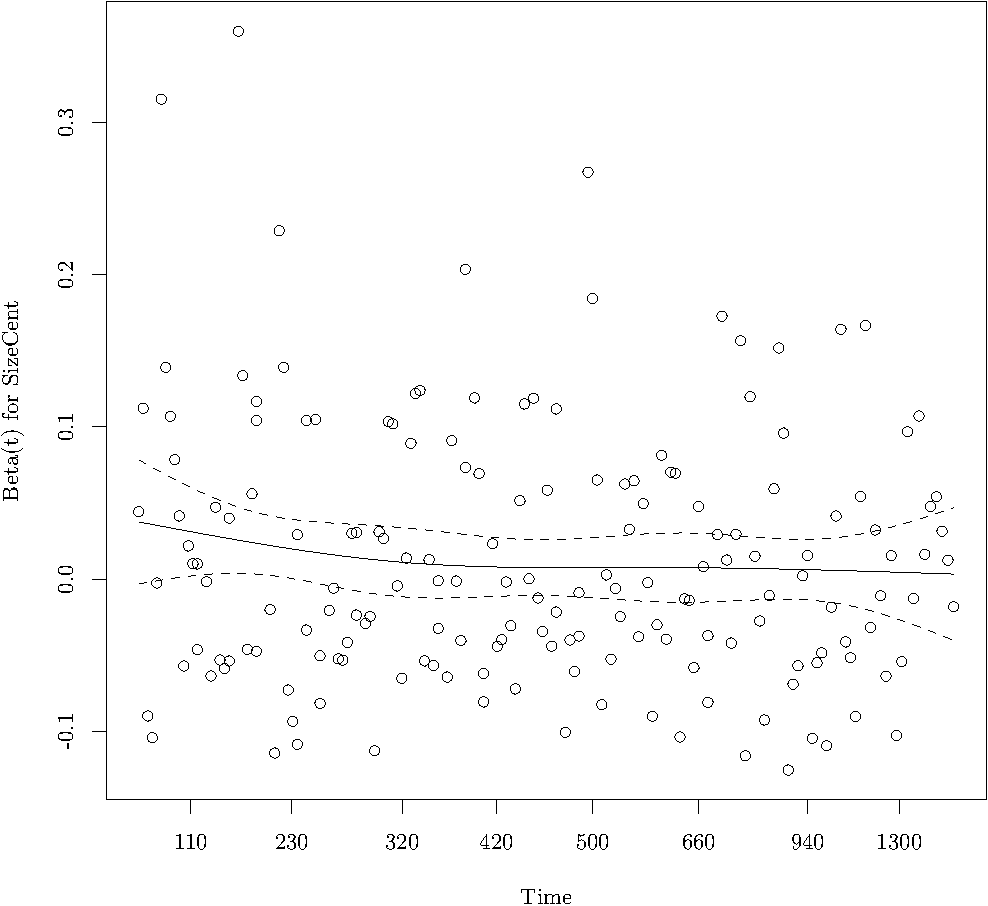
\includegraphics[width=\maxwidth]{figure/05-eda-ph-check-reduced-1} 

}




{\centering 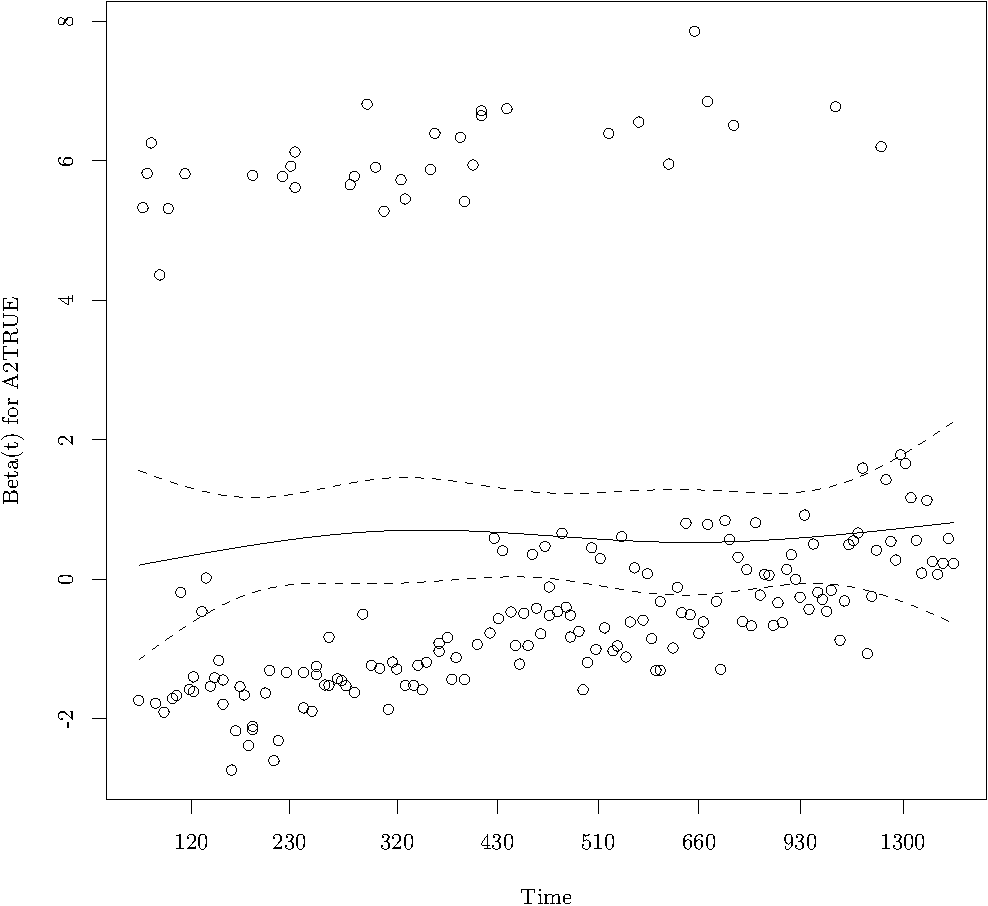
\includegraphics[width=\maxwidth]{figure/05-eda-ph-check-reduced-2} 

}




{\centering 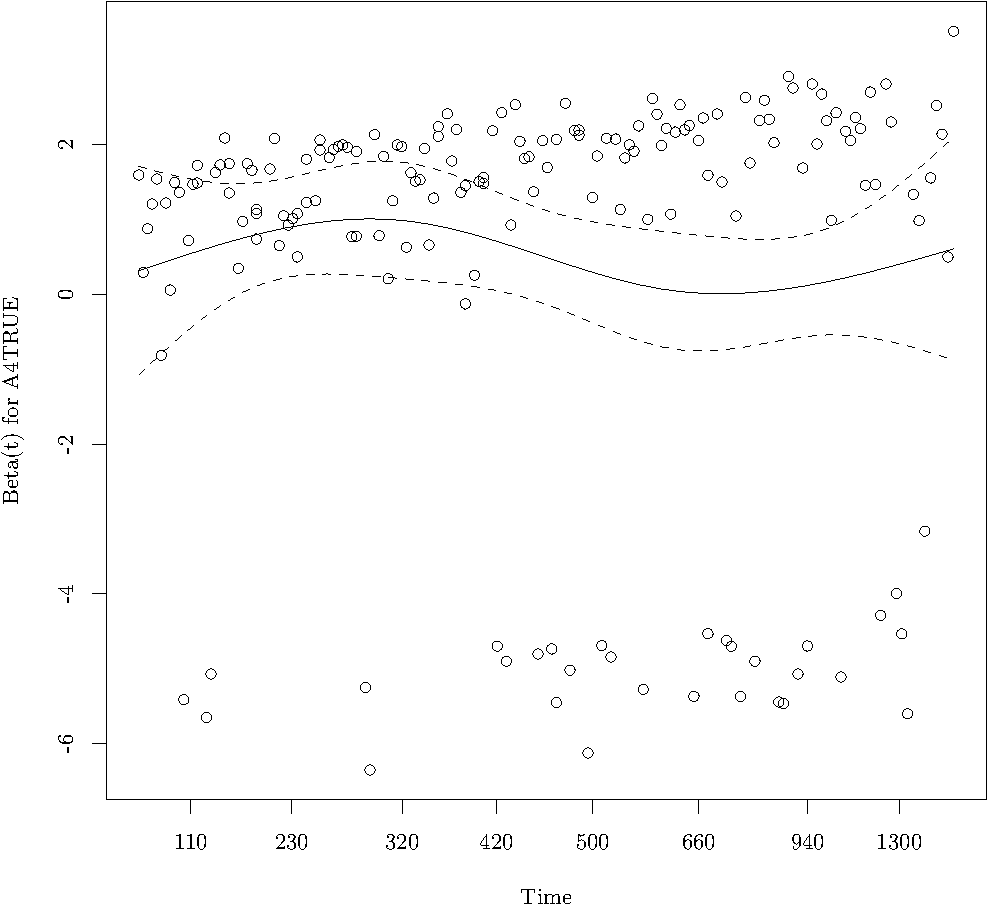
\includegraphics[width=\maxwidth]{figure/05-eda-ph-check-reduced-3} 

}



\end{knitrout}

\subsection{Outliers: reduced model}
\begin{knitrout}
\definecolor{shadecolor}{rgb}{0.969, 0.969, 0.969}\color{fgcolor}\begin{kframe}
\begin{alltt}
\hlkwd{plot}\hlstd{(}\hlkwd{resid}\hlstd{(fit.cph,} \hlkwc{type} \hlstd{=} \hlstr{"deviance"}\hlstd{))}
\end{alltt}
\end{kframe}

{\centering 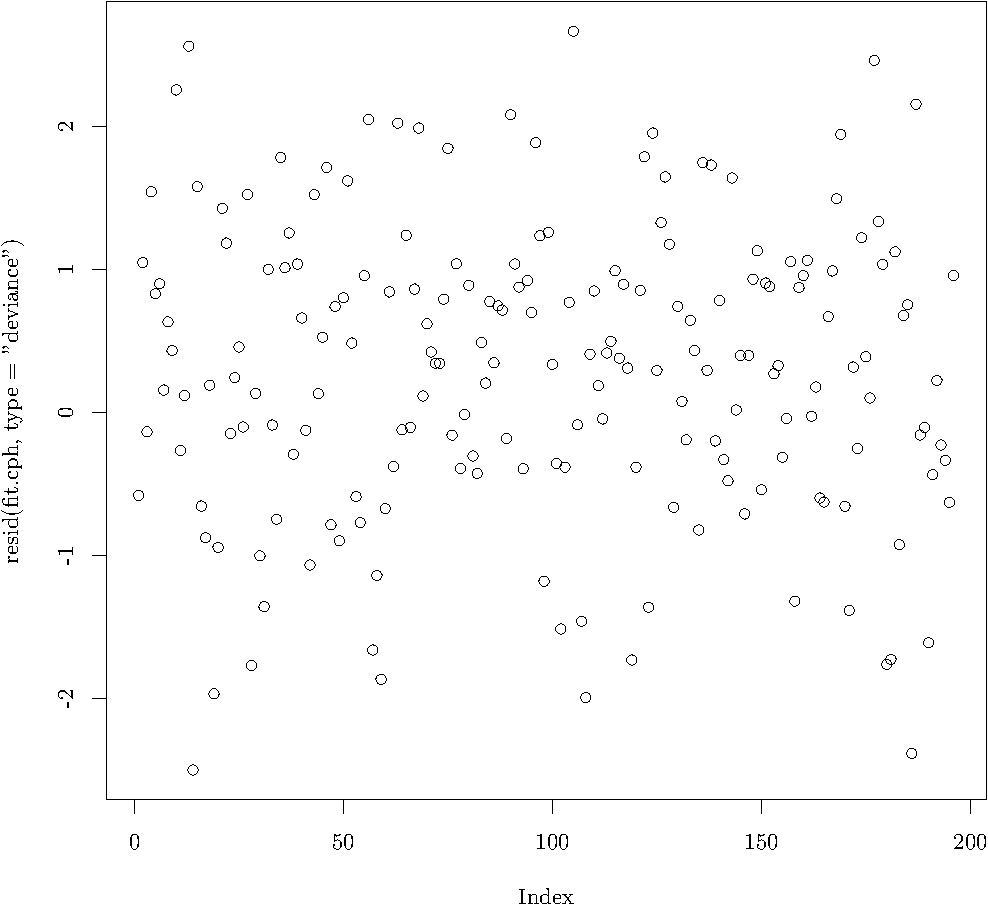
\includegraphics[width=\maxwidth]{figure/05-eda-outliers-reduced-1} 

}



\end{knitrout}

Now generate the restricted fit and examine the DFBETAS on the reduced model.

\begin{knitrout}
\definecolor{shadecolor}{rgb}{0.969, 0.969, 0.969}\color{fgcolor}\begin{kframe}
\begin{alltt}
\hlstd{temp} \hlkwb{=} \hlkwd{resid}\hlstd{(fit.cph,} \hlkwc{type} \hlstd{=} \hlstr{"dfbetas"}\hlstd{)}
\hlkwd{colnames}\hlstd{(temp)} \hlkwb{=} \hlkwd{names}\hlstd{(fit.cph}\hlopt{$}\hlstd{coefficients)}
\hlstd{temp} \hlkwb{=} \hlkwd{melt}\hlstd{(temp)}
\hlkwd{colnames}\hlstd{(temp)} \hlkwb{=} \hlkwd{c}\hlstd{(}\hlstr{"Patient"}\hlstd{,} \hlstr{"Coefficient"}\hlstd{,} \hlstr{"dfbetas"}\hlstd{)}
\hlstd{temp}\hlopt{$}\hlstd{Patient} \hlkwb{=} \hlkwd{gsub}\hlstd{(}\hlstr{"NSWPCN_"}\hlstd{,} \hlstr{""}\hlstd{, temp}\hlopt{$}\hlstd{Patient)}
\hlnum{2}\hlopt{/}\hlkwd{sqrt}\hlstd{(}\hlkwd{nrow}\hlstd{(data))}              \hlcom{# The classic threshold for concern is 2/sqrt(n).}
\end{alltt}
\begin{verbatim}
## [1] 0.1443
\end{verbatim}
\begin{alltt}
\hlkwd{ggplot}\hlstd{(temp,} \hlkwd{aes}\hlstd{(}\hlkwc{y} \hlstd{=} \hlkwd{abs}\hlstd{(dfbetas),} \hlkwc{x} \hlstd{= Patient,} \hlkwc{col} \hlstd{= Coefficient))} \hlopt{+} \hlkwd{geom_point}\hlstd{()} \hlopt{+} \hlkwd{geom_hline}\hlstd{(}\hlkwc{yintercept} \hlstd{=} \hlnum{2}\hlopt{/}\hlkwd{sqrt}\hlstd{(}\hlkwd{nrow}\hlstd{(data)))}
\end{alltt}
\end{kframe}

{\centering 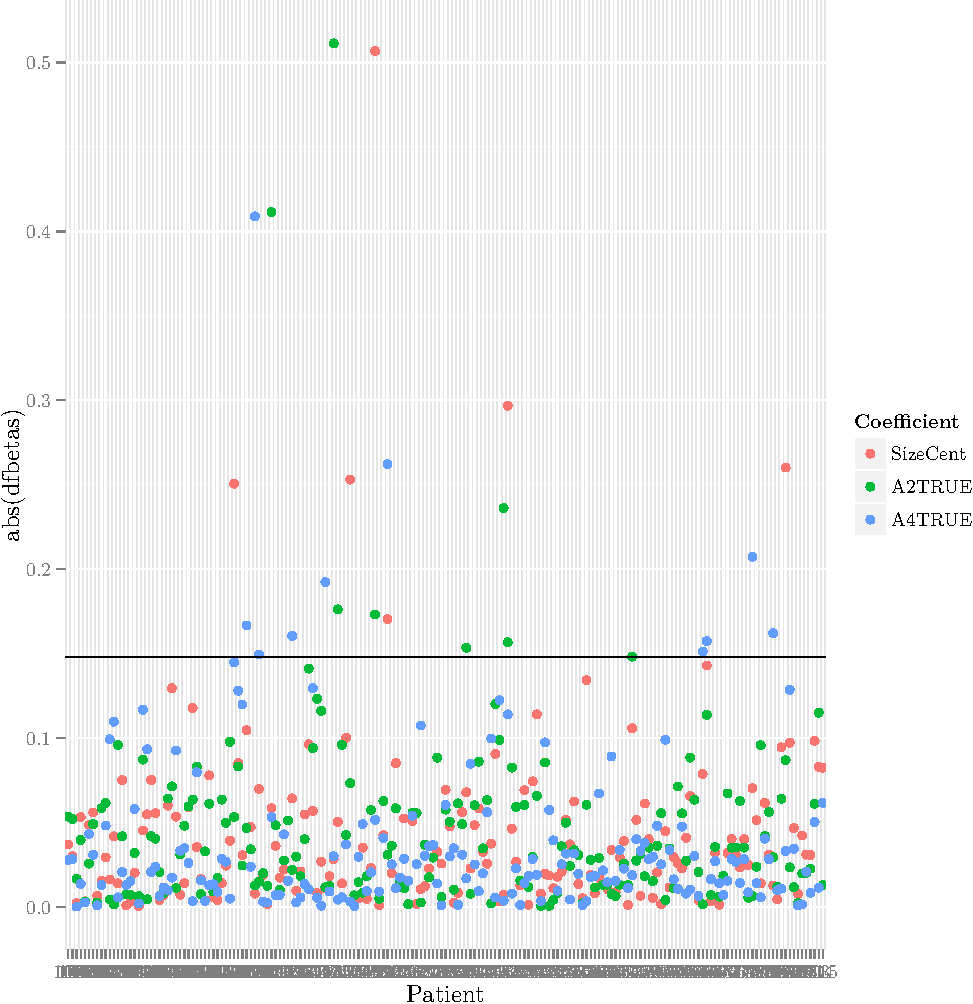
\includegraphics[width=\maxwidth]{figure/05-eda-dfbetas-reduced-1} 

}


\begin{kframe}\begin{alltt}
\hlkwd{sort}\hlstd{(}\hlkwd{apply}\hlstd{(}\hlkwd{abs}\hlstd{(}\hlkwd{resid}\hlstd{(fit.cph,} \hlkwc{type} \hlstd{=} \hlstr{"dfbetas"}\hlstd{)),} \hlnum{1}\hlstd{, max),} \hlkwc{decreasing} \hlstd{=} \hlnum{TRUE}\hlstd{)}
\end{alltt}
\begin{verbatim}
## NSWPCN_1203 NSWPCN_1095  NSWPCN_668  NSWPCN_144 NSWPCN_1212  NSWPCN_183 
##    0.679446    0.577186    0.501923    0.451010    0.396606    0.372111 
## NSWPCN_1253  NSWPCN_154  NSWPCN_799  NSWPCN_788 NSWPCN_1194  NSWPCN_777 
##    0.329044    0.217602    0.214546    0.210311    0.202551    0.188189 
##  NSWPCN_145  NSWPCN_159  NSWPCN_125  NSWPCN_389  NSWPCN_795  NSWPCN_374 
##    0.166285    0.164951    0.154644    0.151544    0.149390    0.147194 
##  NSWPCN_787  NSWPCN_606  NSWPCN_131  NSWPCN_296  NSWPCN_307  NSWPCN_163 
##    0.147006    0.145797    0.140483    0.135732    0.133613    0.130845 
##  NSWPCN_382  NSWPCN_645  NSWPCN_135  NSWPCN_801  NSWPCN_337  NSWPCN_814 
##    0.130554    0.130554    0.126385    0.120654    0.120301    0.119883 
## NSWPCN_1187 NSWPCN_1188  NSWPCN_655  NSWPCN_192 NSWPCN_1155  NSWPCN_313 
##    0.114976    0.113346    0.112513    0.111045    0.109989    0.107328 
## NSWPCN_1182 NSWPCN_1179 NSWPCN_1072  NSWPCN_321  NSWPCN_269  NSWPCN_333 
##    0.103465    0.101334    0.100422    0.099702    0.093907    0.091420 
## NSWPCN_1453 NSWPCN_1082  NSWPCN_639 NSWPCN_1145  NSWPCN_322  NSWPCN_647 
##    0.091302    0.090016    0.089568    0.089343    0.089050    0.088283 
##  NSWPCN_305  NSWPCN_276  NSWPCN_636  NSWPCN_364  NSWPCN_789  NSWPCN_335 
##    0.085957    0.085705    0.084915    0.082950    0.082007    0.081983 
##  NSWPCN_798  NSWPCN_303 NSWPCN_1168  NSWPCN_200  NSWPCN_267  NSWPCN_281 
##    0.079280    0.078363    0.076590    0.072756    0.072372    0.070984 
## NSWPCN_1143  NSWPCN_344 NSWPCN_1189 NSWPCN_1172 NSWPCN_1146  NSWPCN_284 
##    0.070870    0.070489    0.070241    0.067505    0.062471    0.062183 
##  NSWPCN_308 NSWPCN_1177  NSWPCN_257  NSWPCN_348  NSWPCN_326  NSWPCN_815 
##    0.062095    0.061588    0.061508    0.060738    0.060211    0.059693 
##  NSWPCN_377 NSWPCN_1066  NSWPCN_779  NSWPCN_651 NSWPCN_1165 NSWPCN_1213 
##    0.059404    0.059092    0.057056    0.056655    0.056190    0.056140 
##  NSWPCN_324 NSWPCN_1028  NSWPCN_665  NSWPCN_648 NSWPCN_1198  NSWPCN_790 
##    0.056079    0.055128    0.055077    0.055070    0.054993    0.054567 
## NSWPCN_1017 NSWPCN_1029   NSWPCN_10  NSWPCN_182 NSWPCN_1016 NSWPCN_1216 
##    0.053716    0.051710    0.051532    0.051363    0.050528    0.050305 
##  NSWPCN_445  NSWPCN_268 NSWPCN_1031  NSWPCN_663  NSWPCN_351  NSWPCN_360 
##    0.050024    0.050017    0.049762    0.049724    0.049484    0.048131 
##  NSWPCN_769  NSWPCN_643  NSWPCN_336  NSWPCN_661 NSWPCN_1089  NSWPCN_794 
##    0.047896    0.047505    0.046940    0.046846    0.046190    0.045739 
##  NSWPCN_294  NSWPCN_813 NSWPCN_1178   NSWPCN_13 NSWPCN_1183 NSWPCN_1139 
##    0.045642    0.045627    0.045374    0.045292    0.045023    0.045012 
## NSWPCN_1160 NSWPCN_1147 NSWPCN_1019 NSWPCN_1153  NSWPCN_306  NSWPCN_194 
##    0.044393    0.044312    0.043998    0.042885    0.041877    0.040125 
##  NSWPCN_304 NSWPCN_1190  NSWPCN_320   NSWPCN_24  NSWPCN_375  NSWPCN_283 
##    0.039988    0.039368    0.039342    0.038570    0.037468    0.035857 
##  NSWPCN_161 NSWPCN_1075 NSWPCN_1227  NSWPCN_126  NSWPCN_666  NSWPCN_132 
##    0.034647    0.034228    0.033968    0.032846    0.031435    0.030890 
## NSWPCN_1219   NSWPCN_20  NSWPCN_346  NSWPCN_370  NSWPCN_657 NSWPCN_1026 
##    0.030657    0.030628    0.030589    0.030494    0.030390    0.029906 
##    NSWPCN_7  NSWPCN_804 NSWPCN_1021  NSWPCN_273    NSWPCN_4  NSWPCN_376 
##    0.029887    0.029734    0.029387    0.028622    0.028568    0.028157 
## NSWPCN_1158   NSWPCN_21  NSWPCN_384  NSWPCN_811  NSWPCN_781  NSWPCN_369 
##    0.028155    0.027893    0.027871    0.027728    0.027662    0.027516 
## NSWPCN_1141  NSWPCN_280 NSWPCN_1022  NSWPCN_653  NSWPCN_775 NSWPCN_1150 
##    0.027473    0.026816    0.025860    0.025815    0.025492    0.025310 
##  NSWPCN_149  NSWPCN_128 NSWPCN_1152   NSWPCN_36  NSWPCN_810  NSWPCN_638 
##    0.024536    0.024175    0.024113    0.023930    0.023871    0.023853 
##  NSWPCN_646  NSWPCN_309 NSWPCN_1176 NSWPCN_1170  NSWPCN_658  NSWPCN_272 
##    0.023604    0.022866    0.022810    0.022793    0.022659    0.021785 
##  NSWPCN_362 NSWPCN_1173  NSWPCN_656  NSWPCN_352  NSWPCN_807 NSWPCN_1136 
##    0.021164    0.020944    0.020750    0.020673    0.020243    0.020225 
##  NSWPCN_363  NSWPCN_345  NSWPCN_366  NSWPCN_358  NSWPCN_256 NSWPCN_1207 
##    0.019781    0.019100    0.018888    0.018645    0.018451    0.018120 
##  NSWPCN_350  NSWPCN_797  NSWPCN_387  NSWPCN_332  NSWPCN_190  NSWPCN_334 
##    0.017800    0.017032    0.015868    0.015129    0.012700    0.012267 
##  NSWPCN_662  NSWPCN_277  NSWPCN_319  NSWPCN_372  NSWPCN_806 NSWPCN_1211 
##    0.012027    0.011621    0.011569    0.010387    0.010136    0.009291 
##  NSWPCN_330  NSWPCN_373  NSWPCN_136  NSWPCN_157 NSWPCN_1140 NSWPCN_1020 
##    0.008967    0.007566    0.005306    0.003988    0.003038    0.002854
\end{verbatim}
\begin{alltt}
\hlkwd{sum}\hlstd{(}\hlkwd{apply}\hlstd{(}\hlkwd{abs}\hlstd{(}\hlkwd{resid}\hlstd{(fit.cph,} \hlkwc{type} \hlstd{=} \hlstr{"dfbetas"}\hlstd{)),} \hlnum{1}\hlstd{, max)} \hlopt{>} \hlnum{2}\hlopt{/}\hlkwd{sqrt}\hlstd{(}\hlkwd{nrow}\hlstd{(data)))}
\end{alltt}
\begin{verbatim}
## [1] 20
\end{verbatim}
\end{kframe}
\end{knitrout}

\subsection{Summary of EDA}
\begin{enumerate}
\item On the basis of pre-operative assessability and data availability, variables were filtered down to Sex, AgeCent, LocBody, SizeCent, A2, A4.
\item Functional forms for the continuous variates AgeCent and SizeCent indicated a possible slight quadratic effect on AgeCent, and a knee on SizeCent.  These were modelled by incorporating additional terms.
\item Analysis of a full model fit (with additional nonlinear terms included) indicated violation of PH for gender.  This was dealt with by stratification.  A slight PH violation by age was deemed unimportant. 
\item Variable selection by BIC (both stepwise and genetic all-subset) settled on a final model of Surv(Time,DSD) $\sim$ 1 + strata(SexM) + SizeCent + A2 + A4.  This model was refit by coxph. 
\item PH was verified on the final model.  Deviance residuals showed no egregious outliers. dfBetaS indicated a number of influential observations, which require checking.
\end{enumerate}

\section{Final fits}
\begin{knitrout}
\definecolor{shadecolor}{rgb}{0.969, 0.969, 0.969}\color{fgcolor}\begin{kframe}
\begin{alltt}
\hlstd{fit.cph} \hlkwb{=} \hlkwd{coxph}\hlstd{(}\hlkwd{Surv}\hlstd{(Time, DSD)} \hlopt{~} \hlkwd{strata}\hlstd{(SexM)} \hlopt{+} \hlstd{SizeCent} \hlopt{+} \hlstd{A2} \hlopt{+} \hlstd{A4,} \hlkwc{data} \hlstd{= data)}
\end{alltt}
\end{kframe}
\end{knitrout}

\begin{knitrout}
\definecolor{shadecolor}{rgb}{0.969, 0.969, 0.969}\color{fgcolor}\begin{kframe}
\begin{alltt}
\hlkwd{set.seed}\hlstd{(}\hlnum{20150111}\hlstd{)}
\hlstd{fit.rsf} \hlkwb{=} \hlkwd{rfsrc}\hlstd{(}\hlkwd{Surv}\hlstd{(Time, DSD)} \hlopt{~} \hlstd{SexM} \hlopt{+} \hlstd{AgeCent} \hlopt{+} \hlstd{LocBody} \hlopt{+} \hlstd{SizeCent} \hlopt{+} \hlstd{A2} \hlopt{+} \hlstd{A4,} \hlkwc{data} \hlstd{= data,} \hlkwc{mtry} \hlstd{=} \hlnum{1}\hlstd{,} \hlkwc{splitrule} \hlstd{=} \hlstr{"logrankscore"}\hlstd{,} \hlkwc{nsplit} \hlstd{=} \hlnum{2}\hlstd{,} \hlkwc{ntree} \hlstd{=} \hlnum{1000}\hlstd{)}
\end{alltt}
\end{kframe}
\end{knitrout}

\begin{knitrout}
\definecolor{shadecolor}{rgb}{0.969, 0.969, 0.969}\color{fgcolor}\begin{kframe}
\begin{alltt}
\hlstd{fit.gg} \hlkwb{=} \hlkwd{flexsurvreg}\hlstd{(}\hlkwd{Surv}\hlstd{(Time, DSD)} \hlopt{~} \hlstd{SexM} \hlopt{+} \hlstd{SizeCent} \hlopt{+} \hlstd{A2} \hlopt{+} \hlstd{A4,}
        \hlkwc{anc} \hlstd{=} \hlkwd{list}\hlstd{(}
                \hlkwc{sigma} \hlstd{=} \hlopt{~} \hlstd{SexM,}
                \hlkwc{Q} \hlstd{=} \hlopt{~} \hlstd{SexM),}
        \hlkwc{data} \hlstd{= data,} \hlkwc{dist} \hlstd{=} \hlstr{"gengamma"}\hlstd{)}

\hlstd{fit.gf} \hlkwb{=} \hlkwd{flexsurvreg}\hlstd{(}\hlkwd{Surv}\hlstd{(Time, DSD)} \hlopt{~} \hlstd{SexM} \hlopt{+} \hlstd{SizeCent} \hlopt{+} \hlstd{A2} \hlopt{+} \hlstd{A4,}
        \hlkwc{anc} \hlstd{=} \hlkwd{list}\hlstd{(}
                \hlkwc{sigma} \hlstd{=} \hlopt{~} \hlstd{SexM,}
                \hlkwc{Q} \hlstd{=} \hlopt{~} \hlstd{SexM,}
                \hlkwc{P} \hlstd{=} \hlopt{~} \hlstd{SexM),}
        \hlkwc{data} \hlstd{= data,} \hlkwc{dist} \hlstd{=} \hlstr{"genf"}\hlstd{)}

\hlstd{fit.gg}\hlopt{$}\hlstd{loglik}
\end{alltt}
\begin{verbatim}
## [1] -1321
\end{verbatim}
\begin{alltt}
\hlstd{fit.gf}\hlopt{$}\hlstd{loglik}
\end{alltt}
\begin{verbatim}
## [1] -1312
\end{verbatim}
\begin{alltt}
\hlkwd{pchisq}\hlstd{(}\hlnum{2}\hlopt{*}\hlstd{(fit.gf}\hlopt{$}\hlstd{loglik} \hlopt{-} \hlstd{fit.gg}\hlopt{$}\hlstd{loglik),} \hlnum{2}\hlstd{,} \hlkwc{lower.tail} \hlstd{=} \hlnum{FALSE}\hlstd{)}
\end{alltt}
\begin{verbatim}
## [1] 0.0001097
\end{verbatim}
\begin{alltt}
\hlkwd{AIC}\hlstd{(fit.gg)}
\end{alltt}
\begin{verbatim}
## [1] 2660
\end{verbatim}
\begin{alltt}
\hlkwd{AIC}\hlstd{(fit.gf)}
\end{alltt}
\begin{verbatim}
## [1] 2646
\end{verbatim}
\begin{alltt}
\hlkwd{BIC}\hlstd{(fit.gg)}
\end{alltt}
\begin{verbatim}
## [1] 2689
\end{verbatim}
\begin{alltt}
\hlkwd{BIC}\hlstd{(fit.gf)}
\end{alltt}
\begin{verbatim}
## [1] 2682
\end{verbatim}
\begin{alltt}
\hlstd{fit.gg}
\end{alltt}
\begin{verbatim}
## 
## Call:
## flexsurvreg(formula = Surv(Time, DSD) ~ SexM + SizeCent + A2 +     A4, anc = list(sigma = ~SexM, Q = ~SexM), data = data, dist = "gengamma")
## 
## Estimates: 
##                  data mean  est       L95%      U95%      se      
## mu                     NA    6.23934   5.84294   6.63575   0.20225
## sigma                  NA    0.89127   0.76429   1.03933   0.06989
## Q                      NA   -0.55202  -1.04978  -0.05427   0.25396
## SexMTRUE          0.48438    0.42793   0.05650   0.79936   0.18951
## SizeCent          3.65104   -0.01605  -0.02472  -0.00739   0.00442
## A2TRUE            0.17188   -0.37690  -0.70956  -0.04425   0.16972
## A4TRUE            0.78125   -0.31796  -0.62892  -0.00699   0.15866
## sigma(SexMTRUE)   0.48438   -0.04243  -0.26147   0.17661   0.11176
## Q(SexMTRUE)       0.48438    0.73193   0.09949   1.36438   0.32268
##                  exp(est)  L95%      U95%    
## mu                     NA        NA        NA
## sigma                  NA        NA        NA
## Q                      NA        NA        NA
## SexMTRUE          1.53408   1.05813   2.22412
## SizeCent          0.98407   0.97559   0.99264
## A2TRUE            0.68598   0.49186   0.95671
## A4TRUE            0.72764   0.53317   0.99303
## sigma(SexMTRUE)   0.95846   0.76992   1.19316
## Q(SexMTRUE)       2.07909   1.10461   3.91328
## 
## N = 192,  Events: 178,  Censored: 14
## Total time at risk: 133721
## Log-likelihood = -1321, df = 9
## AIC = 2660
\end{verbatim}
\end{kframe}
\end{knitrout}

\section{Fit assessment}
Plot fit stratified by sex, separate curves for A2, A4 status, at median (approx.) Size.
\begin{knitrout}
\definecolor{shadecolor}{rgb}{0.969, 0.969, 0.969}\color{fgcolor}\begin{kframe}
\begin{alltt}
\hlstd{temp.grid} \hlkwb{=} \hlkwd{expand.grid}\hlstd{(}\hlkwc{A4} \hlstd{=} \hlkwd{c}\hlstd{(}\hlnum{FALSE}\hlstd{,} \hlnum{TRUE}\hlstd{),} \hlkwc{A2} \hlstd{=} \hlkwd{c}\hlstd{(}\hlnum{FALSE}\hlstd{,} \hlnum{TRUE}\hlstd{),} \hlkwc{SexM} \hlstd{=} \hlkwd{c}\hlstd{(}\hlnum{FALSE}\hlstd{,} \hlnum{TRUE}\hlstd{),} \hlkwc{SizeCent} \hlstd{=} \hlnum{0}\hlstd{)}
\hlstd{temp.grid}\hlopt{$}\hlstd{ID} \hlkwb{=} \hlkwd{sprintf}\hlstd{(}\hlstr{"SexM=%s, A2=% -5s, A4=% -5s"}\hlstd{, temp.grid}\hlopt{$}\hlstd{SexM, temp.grid}\hlopt{$}\hlstd{A2, temp.grid}\hlopt{$}\hlstd{A4)}
\hlstd{temp.preds} \hlkwb{=} \hlkwd{summary}\hlstd{(fit.gg,} \hlkwc{newdata} \hlstd{= temp.grid,} \hlkwc{type} \hlstd{=} \hlstr{"survival"}\hlstd{,} \hlkwc{t} \hlstd{=} \hlkwd{seq}\hlstd{(}\hlnum{0}\hlstd{,} \hlnum{365}\hlopt{*}\hlnum{5}\hlstd{,} \hlnum{30}\hlstd{))}
\hlstd{temp.preds2} \hlkwb{=} \hlkwd{do.call}\hlstd{(rbind, temp.preds)}
\hlstd{temp.preds2}\hlopt{$}\hlstd{group} \hlkwb{=} \hlkwd{rep}\hlstd{(}\hlkwd{gsub}\hlstd{(}\hlstr{".*ID="}\hlstd{,} \hlstr{""}\hlstd{,} \hlkwd{names}\hlstd{(temp.preds)),} \hlkwc{each} \hlstd{=} \hlkwd{nrow}\hlstd{(temp.preds[[}\hlnum{1}\hlstd{]]))}
\hlstd{temp.preds.cox} \hlkwb{=} \hlkwd{survfit}\hlstd{(fit.cph,} \hlkwc{newdata} \hlstd{= temp.grid)}

\hlstd{temp.survfit} \hlkwb{=} \hlkwd{survfit}\hlstd{(}\hlkwd{Surv}\hlstd{(Time, DSD)} \hlopt{~} \hlstd{SexM} \hlopt{+} \hlstd{A2} \hlopt{+} \hlstd{A4, data)}
\hlstd{temp.data} \hlkwb{=} \hlkwd{data.frame}\hlstd{(}\hlkwc{time} \hlstd{= temp.survfit}\hlopt{$}\hlstd{time,} \hlkwc{surv} \hlstd{= temp.survfit}\hlopt{$}\hlstd{surv,} \hlkwc{upper} \hlstd{= temp.survfit}\hlopt{$}\hlstd{lower,} \hlkwc{lower} \hlstd{= temp.survfit}\hlopt{$}\hlstd{upper,} \hlkwc{group} \hlstd{=} \hlkwd{rep}\hlstd{(}\hlkwd{names}\hlstd{(temp.survfit}\hlopt{$}\hlstd{strata), temp.survfit}\hlopt{$}\hlstd{strata),} \hlkwc{model} \hlstd{=} \hlstr{"KM"}\hlstd{)}
\hlstd{temp.data} \hlkwb{=} \hlkwd{rbind}\hlstd{(temp.data,} \hlkwd{data.frame}\hlstd{(}\hlkwc{time} \hlstd{= temp.preds2}\hlopt{$}\hlstd{time,} \hlkwc{surv} \hlstd{= temp.preds2}\hlopt{$}\hlstd{est,} \hlkwc{upper} \hlstd{= temp.preds2}\hlopt{$}\hlstd{ucl,} \hlkwc{lower} \hlstd{= temp.preds2}\hlopt{$}\hlstd{lcl,} \hlkwc{group} \hlstd{= temp.preds2}\hlopt{$}\hlstd{group,} \hlkwc{model} \hlstd{=} \hlstr{"GG"}\hlstd{))}
\hlstd{temp.data} \hlkwb{=} \hlkwd{rbind}\hlstd{(temp.data,} \hlkwd{data.frame}\hlstd{(}\hlkwc{time} \hlstd{= temp.preds.cox}\hlopt{$}\hlstd{time,} \hlkwc{surv} \hlstd{= temp.preds.cox}\hlopt{$}\hlstd{surv,} \hlkwc{upper} \hlstd{= temp.preds.cox}\hlopt{$}\hlstd{upper,} \hlkwc{lower} \hlstd{= temp.preds.cox}\hlopt{$}\hlstd{lower,} \hlkwc{group} \hlstd{=} \hlkwd{rep}\hlstd{(temp.grid}\hlopt{$}\hlstd{ID, temp.preds.cox}\hlopt{$}\hlstd{strata),} \hlkwc{model} \hlstd{=} \hlstr{"CPH"}\hlstd{))}

\hlstd{temp.data}\hlopt{$}\hlstd{Sex} \hlkwb{=} \hlkwd{c}\hlstd{(}\hlstr{"Male"}\hlstd{,} \hlstr{"Female"}\hlstd{)[}\hlkwd{grepl}\hlstd{(}\hlstr{"SexM=FALSE"}\hlstd{, temp.data}\hlopt{$}\hlstd{group)}\hlopt{+}\hlnum{1}\hlstd{]}
\hlstd{temp.data}\hlopt{$}\hlstd{A2} \hlkwb{=} \hlkwd{c}\hlstd{(}\hlstr{"A2-"}\hlstd{,} \hlstr{"A2+"}\hlstd{)[}\hlkwd{grepl}\hlstd{(}\hlstr{"A2=TRUE"}\hlstd{, temp.data}\hlopt{$}\hlstd{group)}\hlopt{+}\hlnum{1}\hlstd{]}
\hlstd{temp.data}\hlopt{$}\hlstd{A4} \hlkwb{=} \hlkwd{c}\hlstd{(}\hlstr{"A4-"}\hlstd{,} \hlstr{"A4+"}\hlstd{)[}\hlkwd{grepl}\hlstd{(}\hlstr{"A4=TRUE"}\hlstd{, temp.data}\hlopt{$}\hlstd{group)}\hlopt{+}\hlnum{1}\hlstd{]}

\hlkwd{ggplot}\hlstd{(temp.data,} \hlkwd{aes}\hlstd{(}\hlkwc{x} \hlstd{=} \hlkwd{log}\hlstd{(time),} \hlkwc{y} \hlstd{=} \hlkwd{log}\hlstd{(}\hlopt{-}\hlkwd{log}\hlstd{(surv)),} \hlkwc{ymin} \hlstd{=} \hlkwd{log}\hlstd{(}\hlopt{-}\hlkwd{log}\hlstd{(lower)),} \hlkwc{ymax} \hlstd{=} \hlkwd{log}\hlstd{(}\hlopt{-}\hlkwd{log}\hlstd{(upper)),} \hlkwc{colour} \hlstd{= model,} \hlkwc{fill} \hlstd{= model))} \hlopt{+}
        \hlkwd{geom_ribbon}\hlstd{(}\hlkwc{alpha} \hlstd{=} \hlnum{0.25}\hlstd{,} \hlkwc{colour} \hlstd{=} \hlnum{NA}\hlstd{)} \hlopt{+}
        \hlkwd{geom_line}\hlstd{()} \hlopt{+}
        \hlkwd{xlim}\hlstd{(}\hlnum{4}\hlstd{,} \hlnum{7}\hlstd{)} \hlopt{+} \hlkwd{ylim}\hlstd{(}\hlopt{-}\hlnum{4}\hlstd{,} \hlnum{2}\hlstd{)} \hlopt{+}
        \hlkwd{facet_grid}\hlstd{(A2} \hlopt{~} \hlstd{A4} \hlopt{~} \hlstd{Sex)}
\end{alltt}


{\ttfamily\noindent\color{warningcolor}{\#\# Warning: Removed 54 rows containing missing values (geom\_path).}}

{\ttfamily\noindent\color{warningcolor}{\#\# Warning: Removed 41 rows containing missing values (geom\_path).}}

{\ttfamily\noindent\color{warningcolor}{\#\# Warning: Removed 55 rows containing missing values (geom\_path).}}

{\ttfamily\noindent\color{warningcolor}{\#\# Warning: Removed 47 rows containing missing values (geom\_path).}}

{\ttfamily\noindent\color{warningcolor}{\#\# Warning: Removed 44 rows containing missing values (geom\_path).}}

{\ttfamily\noindent\color{warningcolor}{\#\# Warning: Removed 39 rows containing missing values (geom\_path).}}

{\ttfamily\noindent\color{warningcolor}{\#\# Warning: Removed 45 rows containing missing values (geom\_path).}}

{\ttfamily\noindent\color{warningcolor}{\#\# Warning: Removed 38 rows containing missing values (geom\_path).}}\end{kframe}

{\centering 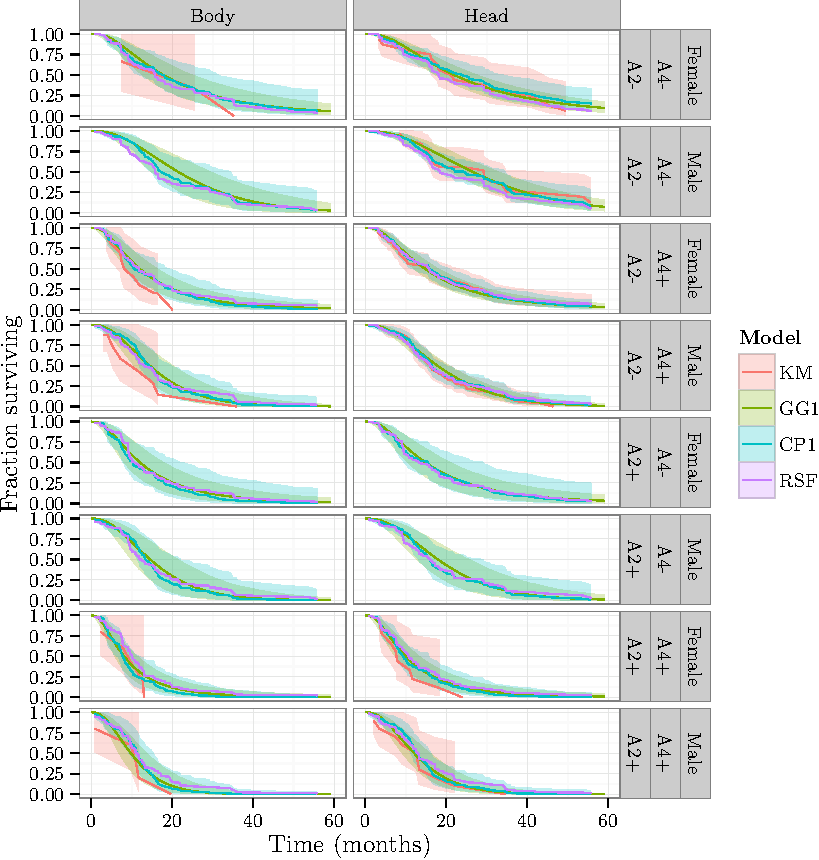
\includegraphics[width=\maxwidth]{figure/05-final-fit-assessment-1} 

}


\begin{kframe}\begin{alltt}
\hlkwd{ggplot}\hlstd{(temp.data,} \hlkwd{aes}\hlstd{(}\hlkwc{x} \hlstd{= time,} \hlkwc{y} \hlstd{= surv,} \hlkwc{ymin} \hlstd{= lower,} \hlkwc{ymax} \hlstd{= upper,} \hlkwc{colour} \hlstd{= model,} \hlkwc{fill} \hlstd{= model))} \hlopt{+}
        \hlkwd{geom_ribbon}\hlstd{(}\hlkwc{alpha} \hlstd{=} \hlnum{0.25}\hlstd{,} \hlkwc{colour} \hlstd{=} \hlnum{NA}\hlstd{)} \hlopt{+}
        \hlkwd{geom_line}\hlstd{()} \hlopt{+} \hlkwd{xlim}\hlstd{(}\hlnum{0}\hlstd{,} \hlnum{2000}\hlstd{)} \hlopt{+} \hlkwd{ylim}\hlstd{(}\hlnum{0}\hlstd{,} \hlnum{1}\hlstd{)} \hlopt{+}
        \hlkwd{facet_grid}\hlstd{(A2} \hlopt{~} \hlstd{A4} \hlopt{~} \hlstd{Sex)}
\end{alltt}


{\ttfamily\noindent\color{warningcolor}{\#\# Warning: Removed 9 rows containing missing values (geom\_path).}}

{\ttfamily\noindent\color{warningcolor}{\#\# Warning: Removed 3 rows containing missing values (geom\_path).}}

{\ttfamily\noindent\color{warningcolor}{\#\# Warning: Removed 12 rows containing missing values (geom\_path).}}

{\ttfamily\noindent\color{warningcolor}{\#\# Warning: Removed 6 rows containing missing values (geom\_path).}}

{\ttfamily\noindent\color{warningcolor}{\#\# Warning: Removed 7 rows containing missing values (geom\_path).}}

{\ttfamily\noindent\color{warningcolor}{\#\# Warning: Removed 3 rows containing missing values (geom\_path).}}

{\ttfamily\noindent\color{warningcolor}{\#\# Warning: Removed 7 rows containing missing values (geom\_path).}}

{\ttfamily\noindent\color{warningcolor}{\#\# Warning: Removed 3 rows containing missing values (geom\_path).}}\end{kframe}

{\centering 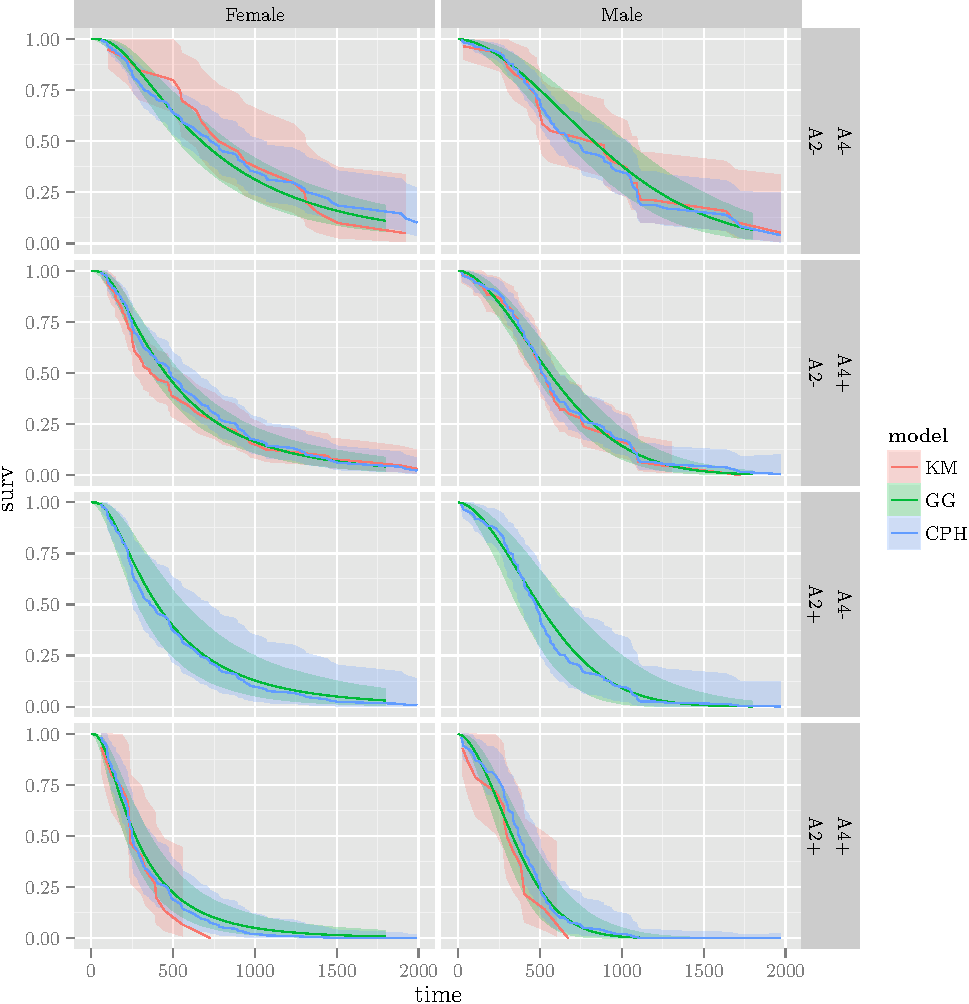
\includegraphics[width=\maxwidth]{figure/05-final-fit-assessment-2} 

}



\end{knitrout}

Some deviation though not significant.  Most concerning is the A2- A4- female group, survival of which is underestimated by the flexsurv model.  To approach this in a modelling sense would require interaction terms between Sex and A2, A4. Overfitting seems likely considering the very few data available for the A2+/A4- group.  Perhaps just add a single "DoubleNegFemale" term.
\begin{knitrout}
\definecolor{shadecolor}{rgb}{0.969, 0.969, 0.969}\color{fgcolor}\begin{kframe}
\begin{alltt}
\hlstd{fit.gg2} \hlkwb{=} \hlkwd{flexsurvreg}\hlstd{(}\hlkwd{Surv}\hlstd{(Time, DSD)} \hlopt{~} \hlstd{SexM} \hlopt{+} \hlstd{SizeCent} \hlopt{+} \hlstd{A2} \hlopt{+} \hlstd{A4} \hlopt{+} \hlkwd{I}\hlstd{(SexM} \hlopt{==} \hlnum{FALSE} \hlopt{&} \hlstd{A2} \hlopt{==} \hlnum{FALSE} \hlopt{&} \hlstd{A4} \hlopt{==} \hlnum{FALSE}\hlstd{),}
        \hlkwc{anc} \hlstd{=} \hlkwd{list}\hlstd{(}
                \hlkwc{sigma} \hlstd{=} \hlopt{~} \hlstd{SexM,}
                \hlkwc{Q} \hlstd{=} \hlopt{~} \hlstd{SexM),}
        \hlkwc{data} \hlstd{= data,} \hlkwc{dist} \hlstd{=} \hlstr{"gengamma"}\hlstd{)}

\hlstd{fit.gg2}
\end{alltt}
\begin{verbatim}
## 
## Call:
## flexsurvreg(formula = Surv(Time, DSD) ~ SexM + SizeCent + A2 +     A4 + I(SexM == FALSE & A2 == FALSE & A4 == FALSE), anc = list(sigma = ~SexM,     Q = ~SexM), data = data, dist = "gengamma")
## 
## Estimates: 
##                                                   data mean  est     
## mu                                                      NA    6.19984
## sigma                                                   NA    0.89245
## Q                                                       NA   -0.53897
## SexMTRUE                                           0.48438    0.44005
## SizeCent                                           3.65104   -0.01596
## A2TRUE                                             0.17188   -0.37310
## A4TRUE                                             0.78125   -0.28237
## I(SexM == FALSE & A2 == FALSE & A4 == FALSE)TRUE   0.09896    0.08326
## sigma(SexMTRUE)                                    0.48438   -0.04436
## Q(SexMTRUE)                                        0.48438    0.72104
##                                                   L95%      U95%    
## mu                                                 5.70768   6.69200
## sigma                                              0.76537   1.04063
## Q                                                 -1.04407  -0.03387
## SexMTRUE                                           0.05832   0.82178
## SizeCent                                          -0.02464  -0.00727
## A2TRUE                                            -0.70757  -0.03863
## A4TRUE                                            -0.68949   0.12476
## I(SexM == FALSE & A2 == FALSE & A4 == FALSE)TRUE  -0.53412   0.70064
## sigma(SexMTRUE)                                   -0.26358   0.17487
## Q(SexMTRUE)                                        0.08448   1.35759
##                                                   se        exp(est)
## mu                                                 0.25111        NA
## sigma                                              0.06994        NA
## Q                                                  0.25771        NA
## SexMTRUE                                           0.19476   1.55278
## SizeCent                                           0.00443   0.98417
## A2TRUE                                             0.17065   0.68860
## A4TRUE                                             0.20772   0.75400
## I(SexM == FALSE & A2 == FALSE & A4 == FALSE)TRUE   0.31499   1.08683
## sigma(SexMTRUE)                                    0.11185   0.95661
## Q(SexMTRUE)                                        0.32478   2.05657
##                                                   L95%      U95%    
## mu                                                      NA        NA
## sigma                                                   NA        NA
## Q                                                       NA        NA
## SexMTRUE                                           1.06005   2.27454
## SizeCent                                           0.97566   0.99275
## A2TRUE                                             0.49284   0.96211
## A4TRUE                                             0.50183   1.13288
## I(SexM == FALSE & A2 == FALSE & A4 == FALSE)TRUE   0.58619   2.01504
## sigma(SexMTRUE)                                    0.76829   1.19109
## Q(SexMTRUE)                                        1.08815   3.88683
## 
## N = 192,  Events: 178,  Censored: 14
## Total time at risk: 133721
## Log-likelihood = -1321, df = 10
## AIC = 2662
\end{verbatim}
\begin{alltt}
\hlkwd{AIC}\hlstd{(fit.gg)}
\end{alltt}
\begin{verbatim}
## [1] 2660
\end{verbatim}
\begin{alltt}
\hlkwd{AIC}\hlstd{(fit.gg2)}
\end{alltt}
\begin{verbatim}
## [1] 2662
\end{verbatim}
\begin{alltt}
\hlkwd{AIC}\hlstd{(fit.gg)} \hlopt{-} \hlkwd{AIC}\hlstd{(fit.gg2)}
\end{alltt}
\begin{verbatim}
## [1] -1.93
\end{verbatim}
\begin{alltt}
\hlcom{# Equivocal on AIC.  BIC would favour gg then.}

\hlkwd{pchisq}\hlstd{(}\hlopt{-}\hlnum{2}\hlopt{*}\hlstd{(fit.gg}\hlopt{$}\hlstd{loglik} \hlopt{-} \hlstd{fit.gg2}\hlopt{$}\hlstd{loglik),} \hlnum{1}\hlstd{,} \hlkwc{lower.tail} \hlstd{=} \hlnum{FALSE}\hlstd{)}
\end{alltt}
\begin{verbatim}
## [1] 0.7917
\end{verbatim}
\begin{alltt}
\hlcom{# Not good evidence on LRT}
\end{alltt}
\end{kframe}
\end{knitrout}

See how it plots relative to the others.
\begin{knitrout}
\definecolor{shadecolor}{rgb}{0.969, 0.969, 0.969}\color{fgcolor}\begin{kframe}
\begin{alltt}
\hlstd{temp.preds} \hlkwb{=} \hlkwd{summary}\hlstd{(fit.gg2,} \hlkwc{newdata} \hlstd{= temp.grid,} \hlkwc{type} \hlstd{=} \hlstr{"survival"}\hlstd{,} \hlkwc{t} \hlstd{=} \hlkwd{seq}\hlstd{(}\hlnum{0}\hlstd{,} \hlnum{365}\hlopt{*}\hlnum{5}\hlstd{,} \hlnum{30}\hlstd{))}
\hlstd{temp.preds2} \hlkwb{=} \hlkwd{do.call}\hlstd{(rbind, temp.preds)}
\hlstd{temp.preds2}\hlopt{$}\hlstd{group} \hlkwb{=} \hlkwd{rep}\hlstd{(}\hlkwd{gsub}\hlstd{(}\hlstr{".*ID="}\hlstd{,} \hlstr{""}\hlstd{,} \hlkwd{names}\hlstd{(temp.preds)),} \hlkwc{each} \hlstd{=} \hlkwd{nrow}\hlstd{(temp.preds[[}\hlnum{1}\hlstd{]]))}
\hlstd{temp.data} \hlkwb{=} \hlkwd{rbind}\hlstd{(temp.data,} \hlkwd{data.frame}\hlstd{(}\hlkwc{time} \hlstd{= temp.preds2}\hlopt{$}\hlstd{time,} \hlkwc{surv} \hlstd{= temp.preds2}\hlopt{$}\hlstd{est,} \hlkwc{upper} \hlstd{= temp.preds2}\hlopt{$}\hlstd{ucl,} \hlkwc{lower} \hlstd{= temp.preds2}\hlopt{$}\hlstd{lcl,} \hlkwc{group} \hlstd{= temp.preds2}\hlopt{$}\hlstd{group,} \hlkwc{model} \hlstd{=} \hlstr{"GG2"}\hlstd{,} \hlkwc{Sex} \hlstd{=} \hlnum{NA}\hlstd{,} \hlkwc{A2} \hlstd{=} \hlnum{NA}\hlstd{,} \hlkwc{A4} \hlstd{=} \hlnum{NA}\hlstd{))}
\hlstd{temp.data}\hlopt{$}\hlstd{Sex} \hlkwb{=} \hlkwd{c}\hlstd{(}\hlstr{"Male"}\hlstd{,} \hlstr{"Female"}\hlstd{)[}\hlkwd{grepl}\hlstd{(}\hlstr{"SexM=FALSE"}\hlstd{, temp.data}\hlopt{$}\hlstd{group)}\hlopt{+}\hlnum{1}\hlstd{]}
\hlstd{temp.data}\hlopt{$}\hlstd{A2} \hlkwb{=} \hlkwd{c}\hlstd{(}\hlstr{"A2-"}\hlstd{,} \hlstr{"A2+"}\hlstd{)[}\hlkwd{grepl}\hlstd{(}\hlstr{"A2=TRUE"}\hlstd{, temp.data}\hlopt{$}\hlstd{group)}\hlopt{+}\hlnum{1}\hlstd{]}
\hlstd{temp.data}\hlopt{$}\hlstd{A4} \hlkwb{=} \hlkwd{c}\hlstd{(}\hlstr{"A4-"}\hlstd{,} \hlstr{"A4+"}\hlstd{)[}\hlkwd{grepl}\hlstd{(}\hlstr{"A4=TRUE"}\hlstd{, temp.data}\hlopt{$}\hlstd{group)}\hlopt{+}\hlnum{1}\hlstd{]}

\hlkwd{ggplot}\hlstd{(temp.data,} \hlkwd{aes}\hlstd{(}\hlkwc{x} \hlstd{=} \hlkwd{log}\hlstd{(time),} \hlkwc{y} \hlstd{=} \hlkwd{log}\hlstd{(}\hlopt{-}\hlkwd{log}\hlstd{(surv)),} \hlkwc{ymin} \hlstd{=} \hlkwd{log}\hlstd{(}\hlopt{-}\hlkwd{log}\hlstd{(lower)),} \hlkwc{ymax} \hlstd{=} \hlkwd{log}\hlstd{(}\hlopt{-}\hlkwd{log}\hlstd{(upper)),} \hlkwc{colour} \hlstd{= model,} \hlkwc{fill} \hlstd{= model))} \hlopt{+}
        \hlkwd{geom_ribbon}\hlstd{(}\hlkwc{alpha} \hlstd{=} \hlnum{0.25}\hlstd{,} \hlkwc{colour} \hlstd{=} \hlnum{NA}\hlstd{)} \hlopt{+}
        \hlkwd{geom_line}\hlstd{()} \hlopt{+}
        \hlkwd{xlim}\hlstd{(}\hlnum{4}\hlstd{,} \hlnum{7}\hlstd{)} \hlopt{+} \hlkwd{ylim}\hlstd{(}\hlopt{-}\hlnum{4}\hlstd{,} \hlnum{2}\hlstd{)} \hlopt{+}
        \hlkwd{facet_grid}\hlstd{(A2} \hlopt{~} \hlstd{A4} \hlopt{~} \hlstd{Sex)}
\end{alltt}


{\ttfamily\noindent\color{warningcolor}{\#\# Warning: Removed 79 rows containing missing values (geom\_path).}}

{\ttfamily\noindent\color{warningcolor}{\#\# Warning: Removed 66 rows containing missing values (geom\_path).}}

{\ttfamily\noindent\color{warningcolor}{\#\# Warning: Removed 80 rows containing missing values (geom\_path).}}

{\ttfamily\noindent\color{warningcolor}{\#\# Warning: Removed 72 rows containing missing values (geom\_path).}}

{\ttfamily\noindent\color{warningcolor}{\#\# Warning: Removed 69 rows containing missing values (geom\_path).}}

{\ttfamily\noindent\color{warningcolor}{\#\# Warning: Removed 64 rows containing missing values (geom\_path).}}

{\ttfamily\noindent\color{warningcolor}{\#\# Warning: Removed 70 rows containing missing values (geom\_path).}}

{\ttfamily\noindent\color{warningcolor}{\#\# Warning: Removed 63 rows containing missing values (geom\_path).}}\end{kframe}

{\centering 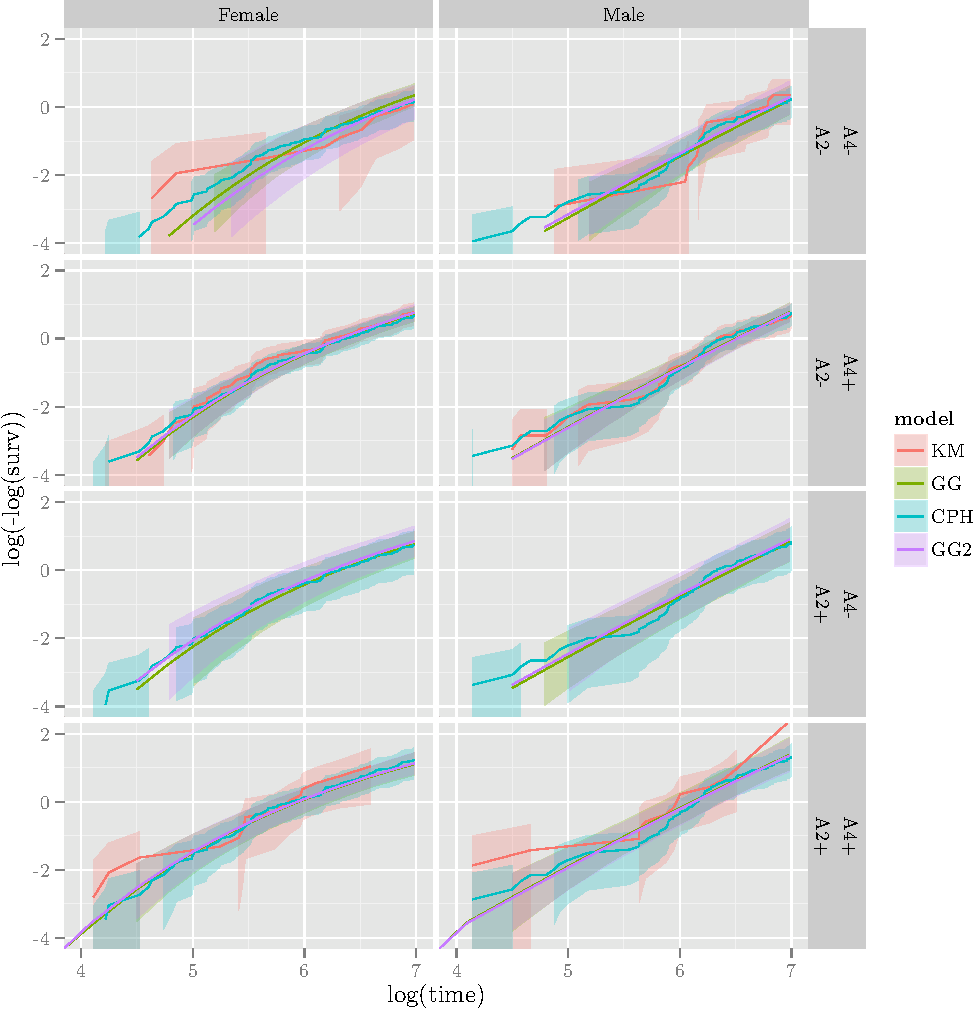
\includegraphics[width=\maxwidth]{figure/05-final-fit-assessment-2-1} 

}


\begin{kframe}\begin{alltt}
\hlkwd{ggplot}\hlstd{(temp.data,} \hlkwd{aes}\hlstd{(}\hlkwc{x} \hlstd{= time,} \hlkwc{y} \hlstd{= surv,} \hlkwc{ymin} \hlstd{= lower,} \hlkwc{ymax} \hlstd{= upper,} \hlkwc{colour} \hlstd{= model,} \hlkwc{fill} \hlstd{= model))} \hlopt{+}
        \hlkwd{geom_ribbon}\hlstd{(}\hlkwc{alpha} \hlstd{=} \hlnum{0.25}\hlstd{,} \hlkwc{colour} \hlstd{=} \hlnum{NA}\hlstd{)} \hlopt{+}
        \hlkwd{geom_line}\hlstd{()} \hlopt{+} \hlkwd{xlim}\hlstd{(}\hlnum{0}\hlstd{,} \hlnum{2000}\hlstd{)} \hlopt{+} \hlkwd{ylim}\hlstd{(}\hlnum{0}\hlstd{,} \hlnum{1}\hlstd{)} \hlopt{+}
        \hlkwd{facet_grid}\hlstd{(A2} \hlopt{~} \hlstd{A4} \hlopt{~} \hlstd{Sex)}
\end{alltt}


{\ttfamily\noindent\color{warningcolor}{\#\# Warning: Removed 9 rows containing missing values (geom\_path).}}

{\ttfamily\noindent\color{warningcolor}{\#\# Warning: Removed 3 rows containing missing values (geom\_path).}}

{\ttfamily\noindent\color{warningcolor}{\#\# Warning: Removed 12 rows containing missing values (geom\_path).}}

{\ttfamily\noindent\color{warningcolor}{\#\# Warning: Removed 6 rows containing missing values (geom\_path).}}

{\ttfamily\noindent\color{warningcolor}{\#\# Warning: Removed 7 rows containing missing values (geom\_path).}}

{\ttfamily\noindent\color{warningcolor}{\#\# Warning: Removed 3 rows containing missing values (geom\_path).}}

{\ttfamily\noindent\color{warningcolor}{\#\# Warning: Removed 7 rows containing missing values (geom\_path).}}

{\ttfamily\noindent\color{warningcolor}{\#\# Warning: Removed 3 rows containing missing values (geom\_path).}}\end{kframe}

{\centering 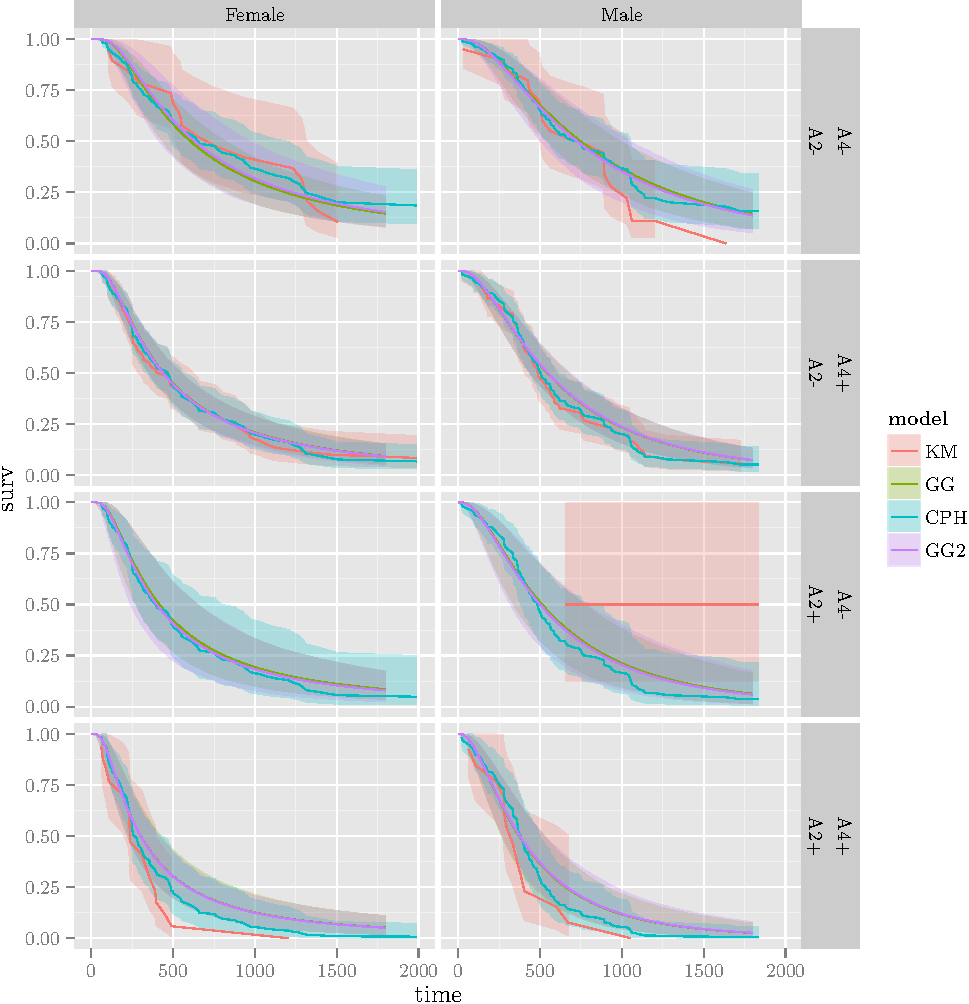
\includegraphics[width=\maxwidth]{figure/05-final-fit-assessment-2-2} 

}



\end{knitrout}

An alternative take, showing errors with the KMs only.
\begin{knitrout}
\definecolor{shadecolor}{rgb}{0.969, 0.969, 0.969}\color{fgcolor}\begin{kframe}
\begin{alltt}
\hlstd{temp.data}\hlopt{$}\hlstd{lower[temp.data}\hlopt{$}\hlstd{model} \hlopt{!=} \hlstr{"KM"}\hlstd{]} \hlkwb{=} \hlnum{NA}
\hlstd{temp.data}\hlopt{$}\hlstd{upper[temp.data}\hlopt{$}\hlstd{model} \hlopt{!=} \hlstr{"KM"}\hlstd{]} \hlkwb{=} \hlnum{NA}
\hlkwd{ggplot}\hlstd{(temp.data,} \hlkwd{aes}\hlstd{(}\hlkwc{x} \hlstd{=} \hlkwd{log}\hlstd{(time),} \hlkwc{y} \hlstd{=} \hlkwd{log}\hlstd{(}\hlopt{-}\hlkwd{log}\hlstd{(surv)),} \hlkwc{ymin} \hlstd{=} \hlkwd{log}\hlstd{(}\hlopt{-}\hlkwd{log}\hlstd{(lower)),} \hlkwc{ymax} \hlstd{=} \hlkwd{log}\hlstd{(}\hlopt{-}\hlkwd{log}\hlstd{(upper)),} \hlkwc{colour} \hlstd{= model,} \hlkwc{fill} \hlstd{= model))} \hlopt{+}
        \hlkwd{geom_ribbon}\hlstd{(}\hlkwc{alpha} \hlstd{=} \hlnum{0.25}\hlstd{,} \hlkwc{colour} \hlstd{=} \hlnum{NA}\hlstd{)} \hlopt{+}
        \hlkwd{geom_line}\hlstd{()} \hlopt{+}
        \hlkwd{xlim}\hlstd{(}\hlnum{4}\hlstd{,} \hlnum{7}\hlstd{)} \hlopt{+} \hlkwd{ylim}\hlstd{(}\hlopt{-}\hlnum{4}\hlstd{,} \hlnum{2}\hlstd{)} \hlopt{+}
        \hlkwd{facet_grid}\hlstd{(A2} \hlopt{~} \hlstd{A4} \hlopt{~} \hlstd{Sex)}
\end{alltt}


{\ttfamily\noindent\color{warningcolor}{\#\# Warning: Removed 79 rows containing missing values (geom\_path).}}

{\ttfamily\noindent\color{warningcolor}{\#\# Warning: Removed 66 rows containing missing values (geom\_path).}}

{\ttfamily\noindent\color{warningcolor}{\#\# Warning: Removed 80 rows containing missing values (geom\_path).}}

{\ttfamily\noindent\color{warningcolor}{\#\# Warning: Removed 72 rows containing missing values (geom\_path).}}

{\ttfamily\noindent\color{warningcolor}{\#\# Warning: Removed 69 rows containing missing values (geom\_path).}}

{\ttfamily\noindent\color{warningcolor}{\#\# Warning: Removed 64 rows containing missing values (geom\_path).}}

{\ttfamily\noindent\color{warningcolor}{\#\# Warning: Removed 70 rows containing missing values (geom\_path).}}

{\ttfamily\noindent\color{warningcolor}{\#\# Warning: Removed 63 rows containing missing values (geom\_path).}}\end{kframe}

{\centering 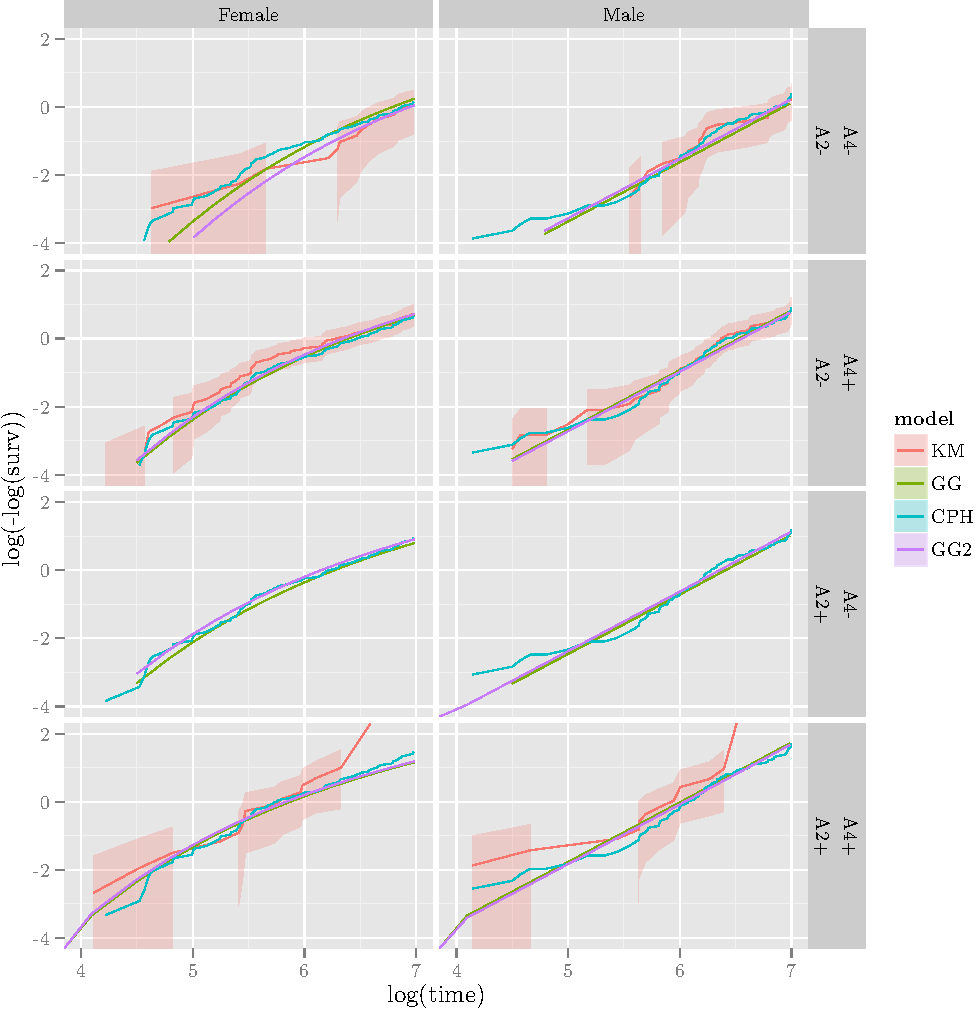
\includegraphics[width=\maxwidth]{figure/05-final-fit-assessment-3-1} 

}


\begin{kframe}\begin{alltt}
\hlkwd{ggplot}\hlstd{(temp.data,} \hlkwd{aes}\hlstd{(}\hlkwc{x} \hlstd{= time,} \hlkwc{y} \hlstd{= surv,} \hlkwc{ymin} \hlstd{= lower,} \hlkwc{ymax} \hlstd{= upper,} \hlkwc{colour} \hlstd{= model,} \hlkwc{fill} \hlstd{= model))} \hlopt{+}
        \hlkwd{geom_ribbon}\hlstd{(}\hlkwc{alpha} \hlstd{=} \hlnum{0.25}\hlstd{,} \hlkwc{colour} \hlstd{=} \hlnum{NA}\hlstd{)} \hlopt{+}
        \hlkwd{geom_line}\hlstd{()} \hlopt{+} \hlkwd{xlim}\hlstd{(}\hlnum{0}\hlstd{,} \hlnum{2000}\hlstd{)} \hlopt{+} \hlkwd{ylim}\hlstd{(}\hlnum{0}\hlstd{,} \hlnum{1}\hlstd{)} \hlopt{+}
        \hlkwd{facet_grid}\hlstd{(A2} \hlopt{~} \hlstd{A4} \hlopt{~} \hlstd{Sex)}
\end{alltt}


{\ttfamily\noindent\color{warningcolor}{\#\# Warning: Removed 9 rows containing missing values (geom\_path).}}

{\ttfamily\noindent\color{warningcolor}{\#\# Warning: Removed 3 rows containing missing values (geom\_path).}}

{\ttfamily\noindent\color{warningcolor}{\#\# Warning: Removed 12 rows containing missing values (geom\_path).}}

{\ttfamily\noindent\color{warningcolor}{\#\# Warning: Removed 6 rows containing missing values (geom\_path).}}

{\ttfamily\noindent\color{warningcolor}{\#\# Warning: Removed 7 rows containing missing values (geom\_path).}}

{\ttfamily\noindent\color{warningcolor}{\#\# Warning: Removed 3 rows containing missing values (geom\_path).}}

{\ttfamily\noindent\color{warningcolor}{\#\# Warning: Removed 7 rows containing missing values (geom\_path).}}

{\ttfamily\noindent\color{warningcolor}{\#\# Warning: Removed 3 rows containing missing values (geom\_path).}}\end{kframe}

{\centering 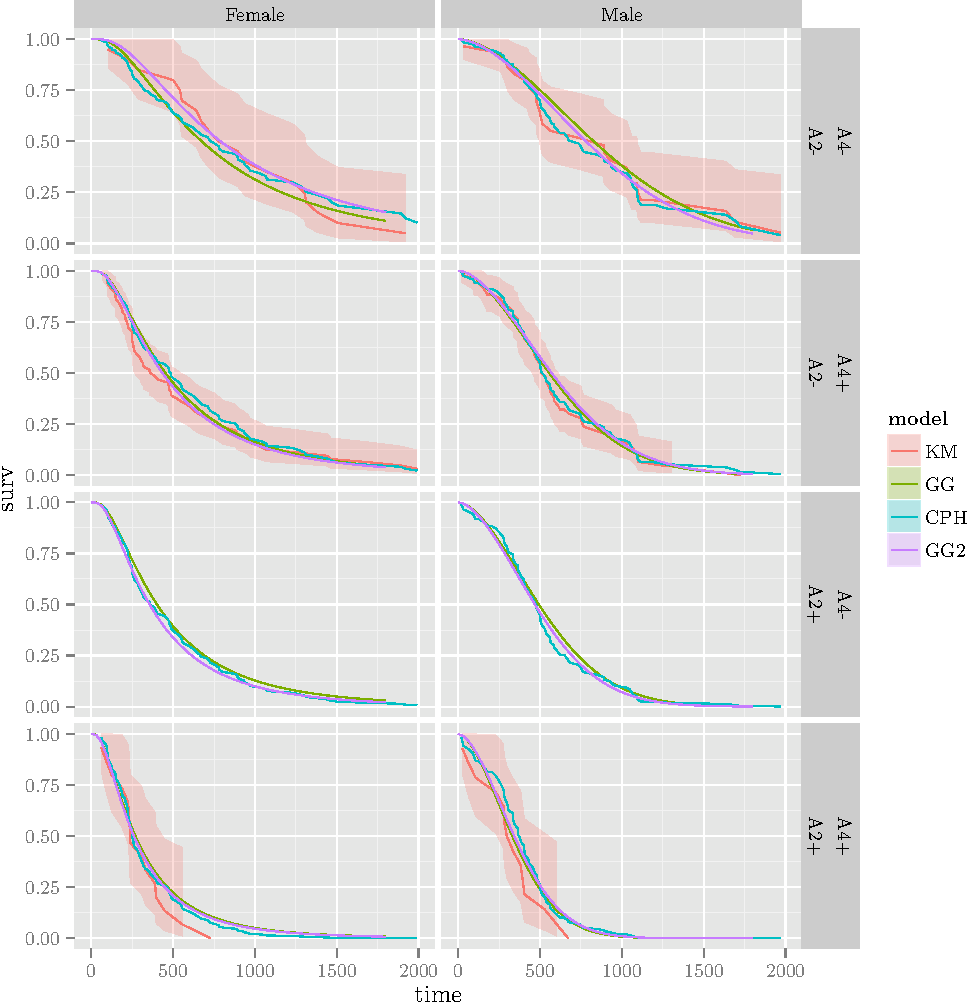
\includegraphics[width=\maxwidth]{figure/05-final-fit-assessment-3-2} 

}



\end{knitrout}

\begin{knitrout}
\definecolor{shadecolor}{rgb}{0.969, 0.969, 0.969}\color{fgcolor}\begin{kframe}
\begin{alltt}
\hlstd{temp.data}\hlopt{$}\hlstd{lower[temp.data}\hlopt{$}\hlstd{model} \hlopt{!=} \hlstr{"KM"}\hlstd{]} \hlkwb{=} \hlnum{NA}
\hlstd{temp.data}\hlopt{$}\hlstd{upper[temp.data}\hlopt{$}\hlstd{model} \hlopt{!=} \hlstr{"KM"}\hlstd{]} \hlkwb{=} \hlnum{NA}
\hlstd{temp.data} \hlkwb{=} \hlstd{temp.data[temp.data}\hlopt{$}\hlstd{model} \hlopt{!=} \hlstr{"GG2"}\hlstd{,]}
\hlstd{temp.data}\hlopt{$}\hlstd{model} \hlkwb{=} \hlkwd{c}\hlstd{(}\hlstr{"KM"} \hlstd{=} \hlstr{"Kaplan-Meier"}\hlstd{,} \hlstr{"GG"} \hlstd{=} \hlstr{"GG1"}\hlstd{,} \hlstr{"CPH"} \hlstd{=} \hlstr{"CP1"}\hlstd{)[temp.data}\hlopt{$}\hlstd{model]}
\hlkwd{ggplot}\hlstd{(temp.data,} \hlkwd{aes}\hlstd{(}\hlkwc{x} \hlstd{=} \hlkwd{log}\hlstd{(time),} \hlkwc{y} \hlstd{=} \hlkwd{log}\hlstd{(}\hlopt{-}\hlkwd{log}\hlstd{(surv)),} \hlkwc{ymin} \hlstd{=} \hlkwd{log}\hlstd{(}\hlopt{-}\hlkwd{log}\hlstd{(lower)),} \hlkwc{ymax} \hlstd{=} \hlkwd{log}\hlstd{(}\hlopt{-}\hlkwd{log}\hlstd{(upper)),} \hlkwc{colour} \hlstd{= model,} \hlkwc{fill} \hlstd{= model))} \hlopt{+}
        \hlkwd{geom_ribbon}\hlstd{(}\hlkwc{alpha} \hlstd{=} \hlnum{0.25}\hlstd{,} \hlkwc{colour} \hlstd{=} \hlnum{NA}\hlstd{)} \hlopt{+}
        \hlkwd{geom_line}\hlstd{()} \hlopt{+}
        \hlkwd{xlim}\hlstd{(}\hlnum{4}\hlstd{,} \hlnum{7}\hlstd{)} \hlopt{+} \hlkwd{ylim}\hlstd{(}\hlopt{-}\hlnum{4}\hlstd{,} \hlnum{2}\hlstd{)} \hlopt{+}
        \hlkwd{facet_grid}\hlstd{(A2} \hlopt{~} \hlstd{A4} \hlopt{~} \hlstd{Sex)}
\end{alltt}


{\ttfamily\noindent\color{warningcolor}{\#\# Warning: Removed 54 rows containing missing values (geom\_path).}}

{\ttfamily\noindent\color{warningcolor}{\#\# Warning: Removed 41 rows containing missing values (geom\_path).}}

{\ttfamily\noindent\color{warningcolor}{\#\# Warning: Removed 55 rows containing missing values (geom\_path).}}

{\ttfamily\noindent\color{warningcolor}{\#\# Warning: Removed 47 rows containing missing values (geom\_path).}}

{\ttfamily\noindent\color{warningcolor}{\#\# Warning: Removed 44 rows containing missing values (geom\_path).}}

{\ttfamily\noindent\color{warningcolor}{\#\# Warning: Removed 39 rows containing missing values (geom\_path).}}

{\ttfamily\noindent\color{warningcolor}{\#\# Warning: Removed 45 rows containing missing values (geom\_path).}}

{\ttfamily\noindent\color{warningcolor}{\#\# Warning: Removed 38 rows containing missing values (geom\_path).}}\end{kframe}

{\centering 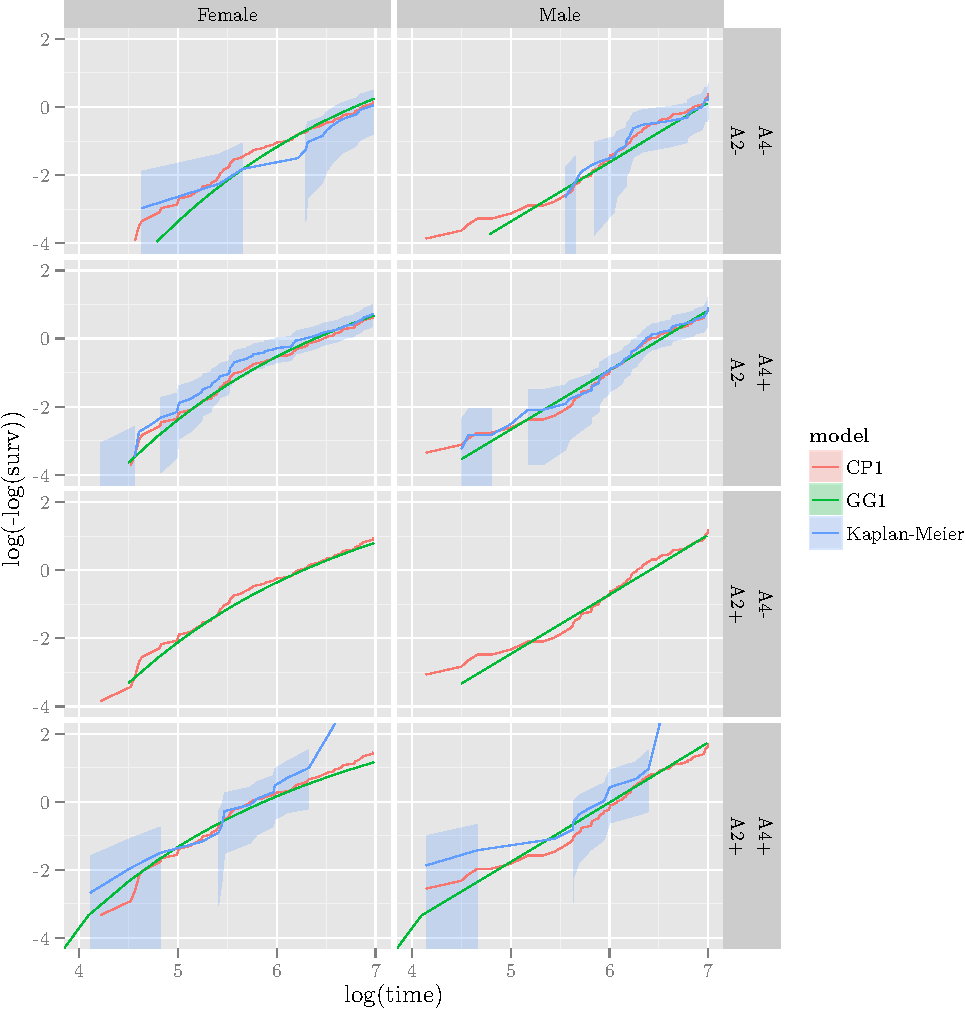
\includegraphics[width=\maxwidth]{figure/05-final-fit-assessment-4-1} 

}


\begin{kframe}\begin{alltt}
\hlkwd{ggplot}\hlstd{(temp.data,} \hlkwd{aes}\hlstd{(}\hlkwc{x} \hlstd{= time,} \hlkwc{y} \hlstd{= surv,} \hlkwc{ymin} \hlstd{= lower,} \hlkwc{ymax} \hlstd{= upper,} \hlkwc{colour} \hlstd{= model,} \hlkwc{fill} \hlstd{= model))} \hlopt{+}
        \hlkwd{geom_ribbon}\hlstd{(}\hlkwc{alpha} \hlstd{=} \hlnum{0.25}\hlstd{,} \hlkwc{colour} \hlstd{=} \hlnum{NA}\hlstd{)} \hlopt{+}
        \hlkwd{geom_line}\hlstd{()} \hlopt{+} \hlkwd{xlim}\hlstd{(}\hlnum{0}\hlstd{,} \hlnum{2000}\hlstd{)} \hlopt{+} \hlkwd{ylim}\hlstd{(}\hlnum{0}\hlstd{,} \hlnum{1}\hlstd{)} \hlopt{+}
        \hlkwd{facet_grid}\hlstd{(A2} \hlopt{~} \hlstd{A4} \hlopt{~} \hlstd{Sex)}
\end{alltt}


{\ttfamily\noindent\color{warningcolor}{\#\# Warning: Removed 9 rows containing missing values (geom\_path).}}

{\ttfamily\noindent\color{warningcolor}{\#\# Warning: Removed 3 rows containing missing values (geom\_path).}}

{\ttfamily\noindent\color{warningcolor}{\#\# Warning: Removed 12 rows containing missing values (geom\_path).}}

{\ttfamily\noindent\color{warningcolor}{\#\# Warning: Removed 6 rows containing missing values (geom\_path).}}

{\ttfamily\noindent\color{warningcolor}{\#\# Warning: Removed 7 rows containing missing values (geom\_path).}}

{\ttfamily\noindent\color{warningcolor}{\#\# Warning: Removed 3 rows containing missing values (geom\_path).}}

{\ttfamily\noindent\color{warningcolor}{\#\# Warning: Removed 7 rows containing missing values (geom\_path).}}

{\ttfamily\noindent\color{warningcolor}{\#\# Warning: Removed 3 rows containing missing values (geom\_path).}}\end{kframe}

{\centering 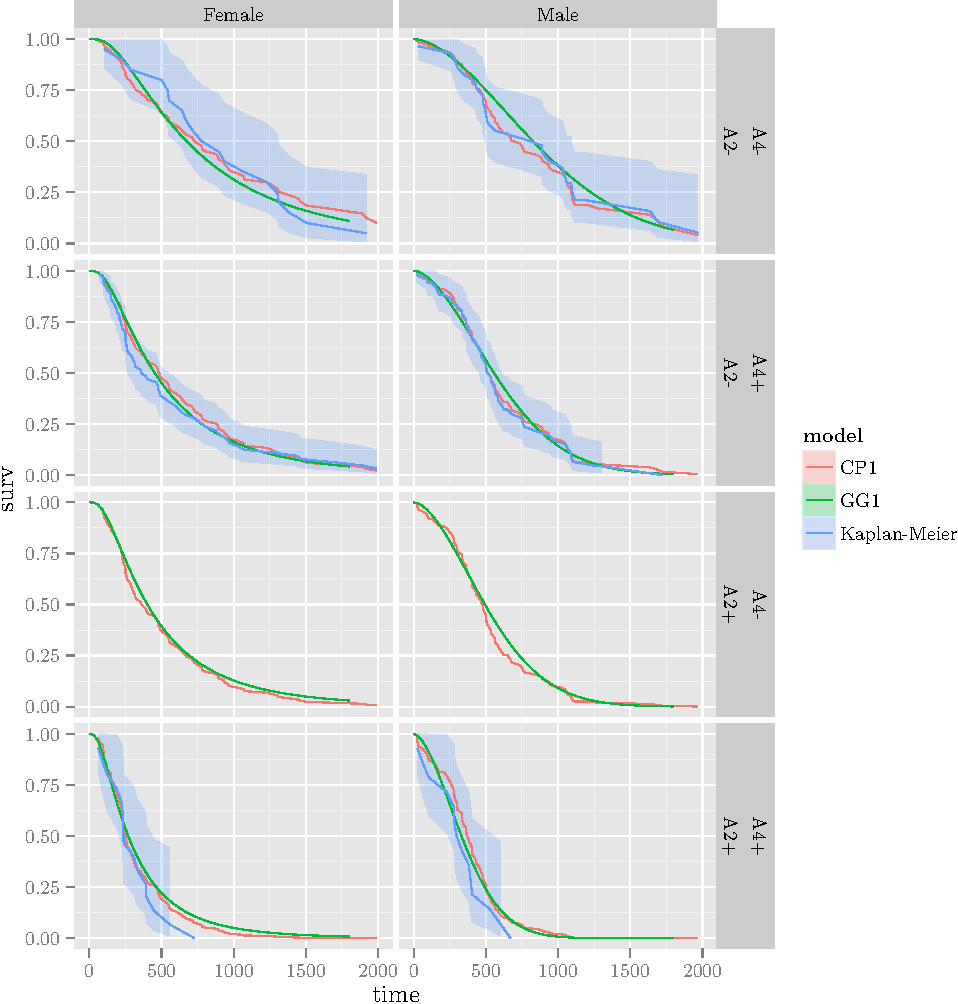
\includegraphics[width=\maxwidth]{figure/05-final-fit-assessment-4-2} 

}



\end{knitrout}


\section{Model selection}
It looks like that's as far as we can go with tweaking the fits.  Time to put the different models against each other on the holdout data, and choose a winner.

DIY IBS, wooo.
\begin{knitrout}
\definecolor{shadecolor}{rgb}{0.969, 0.969, 0.969}\color{fgcolor}\begin{kframe}
\begin{alltt}
\hlstd{calcIBS} \hlkwb{=} \hlkwa{function}\hlstd{(}\hlkwc{surv}\hlstd{,} \hlkwc{pred}\hlstd{,} \hlkwc{pred_times}\hlstd{,} \hlkwc{max_time}\hlstd{)}
\hlstd{\{}
        \hlkwd{stopifnot}\hlstd{(}\hlkwd{nrow}\hlstd{(surv)} \hlopt{==} \hlkwd{nrow}\hlstd{(pred)} \hlopt{&&} \hlkwd{length}\hlstd{(pred_times)} \hlopt{==} \hlkwd{ncol}\hlstd{(pred))}

        \hlstd{n} \hlkwb{=} \hlkwd{nrow}\hlstd{(surv)}
        \hlstd{marg_survfit} \hlkwb{=} \hlkwd{survfit}\hlstd{(surv} \hlopt{~} \hlnum{1}\hlstd{)}
        \hlstd{marg_censfit} \hlkwb{=} \hlkwd{survfit}\hlstd{(}\hlkwd{Surv}\hlstd{(surv[,}\hlnum{1}\hlstd{],} \hlopt{!}\hlstd{surv[,}\hlnum{2}\hlstd{])} \hlopt{~} \hlnum{1}\hlstd{)}
        \hlstd{marg_surv_func} \hlkwb{=} \hlkwd{approxfun}\hlstd{(marg_survfit}\hlopt{$}\hlstd{time, marg_survfit}\hlopt{$}\hlstd{surv,} \hlkwc{method} \hlstd{=} \hlstr{"constant"}\hlstd{,} \hlkwc{yleft} \hlstd{=} \hlnum{1}\hlstd{,} \hlkwc{yright} \hlstd{=} \hlnum{0}\hlstd{,} \hlkwc{rule} \hlstd{=} \hlnum{2}\hlopt{:}\hlnum{1}\hlstd{,} \hlkwc{f} \hlstd{=} \hlnum{0}\hlstd{)}
        \hlstd{marg_cens_func} \hlkwb{=} \hlkwd{approxfun}\hlstd{(marg_censfit}\hlopt{$}\hlstd{time, marg_censfit}\hlopt{$}\hlstd{surv,} \hlkwc{method} \hlstd{=} \hlstr{"constant"}\hlstd{,} \hlkwc{yleft} \hlstd{=} \hlnum{1}\hlstd{,} \hlkwc{yright} \hlstd{=} \hlnum{0}\hlstd{,} \hlkwc{rule} \hlstd{=} \hlnum{2}\hlopt{:}\hlnum{1}\hlstd{,} \hlkwc{f} \hlstd{=} \hlnum{0}\hlstd{)}

        \hlstd{pred_funcs} \hlkwb{=} \hlkwd{apply}\hlstd{(pred,} \hlnum{1}\hlstd{,} \hlkwa{function}\hlstd{(}\hlkwc{pat_preds}\hlstd{)} \hlkwd{approxfun}\hlstd{(pred_times, pat_preds,} \hlkwc{yleft} \hlstd{=} \hlnum{1}\hlstd{,} \hlkwc{yright} \hlstd{=} \hlkwd{min}\hlstd{(pat_preds),} \hlkwc{rule} \hlstd{=} \hlnum{2}\hlstd{))}

        \hlstd{indiv_patient_bsc} \hlkwb{=} \hlkwa{function}\hlstd{(}\hlkwc{pat_i}\hlstd{,} \hlkwc{tstars}\hlstd{)}
        \hlstd{\{}
                \hlstd{observed_time} \hlkwb{=} \hlstd{surv[pat_i,} \hlnum{1}\hlstd{]}
                \hlstd{observed_event} \hlkwb{=} \hlstd{surv[pat_i,} \hlnum{2}\hlstd{]}
                \hlstd{pred_func} \hlkwb{=} \hlstd{pred_funcs[[pat_i]]}
                \hlstd{category} \hlkwb{=} \hlnum{1}\hlopt{*}\hlstd{(observed_time} \hlopt{<=} \hlstd{tstars} \hlopt{&} \hlstd{observed_event)} \hlopt{+} \hlnum{2}\hlopt{*}\hlstd{(observed_time} \hlopt{>} \hlstd{tstars)} \hlopt{+} \hlnum{3}\hlopt{*}\hlstd{(observed_time} \hlopt{<=} \hlstd{tstars} \hlopt{& !}\hlstd{observed_event)}
                \hlstd{bsc} \hlkwb{=} \hlkwd{rep}\hlstd{(}\hlnum{NA}\hlstd{,} \hlkwd{length}\hlstd{(tstars))}
                \hlstd{bsc[category} \hlopt{==} \hlnum{1}\hlstd{]} \hlkwb{=} \hlkwd{pred_func}\hlstd{(tstars[category} \hlopt{==} \hlnum{1}\hlstd{])}\hlopt{^}\hlnum{2} \hlopt{/} \hlkwd{marg_cens_func}\hlstd{(observed_time)}
                \hlstd{bsc[category} \hlopt{==} \hlnum{2}\hlstd{]} \hlkwb{=} \hlstd{(}\hlnum{1} \hlopt{-} \hlkwd{pred_func}\hlstd{(tstars[category} \hlopt{==} \hlnum{2}\hlstd{]))}\hlopt{^}\hlnum{2} \hlopt{/} \hlkwd{marg_cens_func}\hlstd{(tstars[category} \hlopt{==} \hlnum{2}\hlstd{])}
                \hlstd{bsc[category} \hlopt{==} \hlnum{3}\hlstd{]} \hlkwb{=} \hlnum{0}
                \hlstd{bsc}
        \hlstd{\}}

        \hlstd{bsc_func} \hlkwb{=} \hlkwa{function}\hlstd{(}\hlkwc{tstars}\hlstd{) \{} \hlkwd{rowMeans}\hlstd{(}\hlkwd{sapply}\hlstd{(}\hlnum{1}\hlopt{:}\hlstd{n,} \hlkwa{function}\hlstd{(}\hlkwc{pat_i}\hlstd{)} \hlkwd{indiv_patient_bsc}\hlstd{(pat_i, tstars))) \}}

        \hlstd{weight_func} \hlkwb{=} \hlkwa{function}\hlstd{(}\hlkwc{tstars}\hlstd{) \{ (}\hlnum{1} \hlopt{-} \hlkwd{marg_surv_func}\hlstd{(tstars))} \hlopt{/} \hlstd{(}\hlnum{1} \hlopt{-} \hlkwd{marg_surv_func}\hlstd{(max_time)) \}}

        \hlcom{# Be slack and do trapezoidal int. with a fine grid.  It should be possible }
        \hlcom{# to calulate the int. exactly but I cbfed.}
        \hlstd{int_grid} \hlkwb{=} \hlkwd{seq}\hlstd{(}\hlnum{0}\hlstd{, max_time,} \hlkwc{length.out} \hlstd{=} \hlnum{1e3}\hlstd{)}
        \hlstd{bsc_vals} \hlkwb{=} \hlkwd{bsc_func}\hlstd{(int_grid)}
        \hlstd{weight_vals} \hlkwb{=} \hlkwd{weight_func}\hlstd{(int_grid)}
        \hlstd{int_vals} \hlkwb{=} \hlstd{bsc_vals} \hlopt{*} \hlstd{weight_vals}
        \hlstd{ibsc} \hlkwb{=} \hlstd{(}\hlnum{2}\hlopt{*}\hlkwd{sum}\hlstd{(int_vals)} \hlopt{-} \hlstd{int_vals[}\hlnum{1}\hlstd{]} \hlopt{-} \hlstd{int_vals[}\hlkwd{length}\hlstd{(int_vals)])} \hlopt{*} \hlstd{(}\hlkwd{diff}\hlstd{(}\hlkwd{range}\hlstd{(int_grid)))} \hlopt{/} \hlstd{(}\hlnum{2}\hlopt{*}\hlkwd{length}\hlstd{(int_vals))}

        \hlkwd{return}\hlstd{(}\hlkwd{list}\hlstd{(}\hlkwc{bsc} \hlstd{= bsc_vals,} \hlkwc{weights} \hlstd{= weight_vals,} \hlkwc{eval_times} \hlstd{= int_grid,} \hlkwc{ibsc} \hlstd{= ibsc))}
\hlstd{\}}
\end{alltt}
\end{kframe}
\end{knitrout}

Calculate survival probability predictions for each of the models, on the validation data.
\begin{knitrout}
\definecolor{shadecolor}{rgb}{0.969, 0.969, 0.969}\color{fgcolor}\begin{kframe}
\begin{alltt}
\hlstd{ibs_times} \hlkwb{=} \hlkwd{sort}\hlstd{(}\hlkwd{unique}\hlstd{(data.val}\hlopt{$}\hlstd{Time))}
\hlstd{ibs_preds_gg} \hlkwb{=} \hlkwd{as.matrix}\hlstd{(}\hlkwd{t}\hlstd{(}\hlkwd{sapply}\hlstd{(}\hlkwd{summary}\hlstd{(fit.gg,} \hlkwc{newdata} \hlstd{= data.val,} \hlkwc{type} \hlstd{=} \hlstr{"survival"}\hlstd{,} \hlkwc{t} \hlstd{= ibs_times),} \hlkwa{function}\hlstd{(}\hlkwc{x}\hlstd{) x}\hlopt{$}\hlstd{est)))}
\hlstd{ibs_preds_gg2} \hlkwb{=} \hlkwd{as.matrix}\hlstd{(}\hlkwd{t}\hlstd{(}\hlkwd{sapply}\hlstd{(}\hlkwd{summary}\hlstd{(fit.gg2,} \hlkwc{newdata} \hlstd{= data.val,} \hlkwc{type} \hlstd{=} \hlstr{"survival"}\hlstd{,} \hlkwc{t} \hlstd{= ibs_times),} \hlkwa{function}\hlstd{(}\hlkwc{x}\hlstd{) x}\hlopt{$}\hlstd{est)))}
\hlstd{temp_cox_preds} \hlkwb{=} \hlkwd{survfit}\hlstd{(fit.cph,} \hlkwc{newdata} \hlstd{= data.val)}
\hlstd{ibs_preds_cph} \hlkwb{=} \hlkwd{simplify2array}\hlstd{(}\hlkwd{tapply}\hlstd{(}\hlnum{1}\hlopt{:}\hlkwd{length}\hlstd{(temp_cox_preds}\hlopt{$}\hlstd{time),} \hlkwd{rep}\hlstd{(}\hlkwd{names}\hlstd{(temp_cox_preds}\hlopt{$}\hlstd{strata), temp_cox_preds}\hlopt{$}\hlstd{strata),} \hlkwa{function}\hlstd{(}\hlkwc{strat_i}\hlstd{) \{}
        \hlkwd{approx}\hlstd{(}\hlkwc{x} \hlstd{= temp_cox_preds}\hlopt{$}\hlstd{time[strat_i],} \hlkwc{y} \hlstd{= temp_cox_preds}\hlopt{$}\hlstd{surv[strat_i],} \hlkwc{xout} \hlstd{= ibs_times,} \hlkwc{method} \hlstd{=} \hlstr{"constant"}\hlstd{,} \hlkwc{yleft} \hlstd{=} \hlnum{1}\hlstd{,} \hlkwc{rule} \hlstd{=} \hlnum{2}\hlstd{,} \hlkwc{f} \hlstd{=} \hlnum{0}\hlstd{)}\hlopt{$}\hlstd{y \} ))}
\hlstd{ibs_preds_cph} \hlkwb{=} \hlkwd{t}\hlstd{(ibs_preds_cph[,}\hlkwd{rownames}\hlstd{(data.val)])}
\hlstd{temp_rsf_preds} \hlkwb{=} \hlkwd{predict}\hlstd{(fit.rsf,} \hlkwc{newdata} \hlstd{= data.val)}
\hlstd{ibs_preds_rsf} \hlkwb{=} \hlkwd{t}\hlstd{(}\hlkwd{apply}\hlstd{(temp_rsf_preds}\hlopt{$}\hlstd{survival,} \hlnum{1}\hlstd{,} \hlkwa{function}\hlstd{(}\hlkwc{survs}\hlstd{)} \hlkwd{approx}\hlstd{(temp_rsf_preds}\hlopt{$}\hlstd{time.interest, survs,} \hlkwc{xout} \hlstd{= ibs_times,} \hlkwc{method} \hlstd{=} \hlstr{"constant"}\hlstd{,} \hlkwc{yleft} \hlstd{=} \hlnum{1}\hlstd{,} \hlkwc{rule} \hlstd{=} \hlnum{2}\hlstd{,} \hlkwc{f} \hlstd{=} \hlnum{0}\hlstd{)}\hlopt{$}\hlstd{y))}
\hlcom{# Patients (from data.val) are in rows, times (from ibs_times) in columns.}

\hlcom{# Add a no-information KM predictor}
\hlstd{temp_km0} \hlkwb{=} \hlkwd{survfit}\hlstd{(}\hlkwd{Surv}\hlstd{(Time, DSD)} \hlopt{~} \hlnum{1}\hlstd{, data)}
\hlstd{ibs_preds_km0} \hlkwb{=} \hlkwd{t}\hlstd{(}\hlkwd{matrix}\hlstd{(}\hlkwd{rep}\hlstd{(}\hlkwd{approx}\hlstd{(temp_km0}\hlopt{$}\hlstd{time, temp_km0}\hlopt{$}\hlstd{surv,} \hlkwc{xout} \hlstd{= ibs_times,} \hlkwc{method} \hlstd{=} \hlstr{"constant"}\hlstd{,} \hlkwc{yleft} \hlstd{=} \hlnum{1}\hlstd{,} \hlkwc{rule} \hlstd{=} \hlnum{2}\hlstd{,} \hlkwc{f} \hlstd{=} \hlnum{0}\hlstd{)}\hlopt{$}\hlstd{y,} \hlkwc{times} \hlstd{=} \hlkwd{nrow}\hlstd{(data.val)),} \hlkwc{ncol} \hlstd{=} \hlkwd{nrow}\hlstd{(data.val)))}
\hlstd{ibs_preds_all} \hlkwb{=} \hlkwd{list}\hlstd{(}\hlkwc{gg} \hlstd{= ibs_preds_gg,} \hlkwc{gg2} \hlstd{= ibs_preds_gg2,} \hlkwc{cph} \hlstd{= ibs_preds_cph,} \hlkwc{rsf} \hlstd{= ibs_preds_rsf,} \hlkwc{km0} \hlstd{= ibs_preds_km0)}
\end{alltt}
\end{kframe}
\end{knitrout}


\begin{knitrout}
\definecolor{shadecolor}{rgb}{0.969, 0.969, 0.969}\color{fgcolor}\begin{kframe}
\begin{alltt}
\hlstd{val.prob.times} \hlkwb{=} \hlkwd{seq}\hlstd{(}\hlnum{0}\hlstd{,} \hlkwd{max}\hlstd{(data.val}\hlopt{$}\hlstd{Time),} \hlnum{1}\hlstd{)}

\hlstd{temp.coefs} \hlkwb{=} \hlkwd{coef}\hlstd{(fit.gg)}
\hlstd{val.linpred.gg} \hlkwb{=} \hlkwd{sapply}\hlstd{(}\hlnum{1}\hlopt{:}\hlkwd{length}\hlstd{(temp.coefs),} \hlkwa{function}\hlstd{(}\hlkwc{coef_i}\hlstd{) \{}
    \hlkwa{if} \hlstd{(}\hlkwd{names}\hlstd{(temp.coefs)[coef_i]} \hlopt \hlkwd{colnames}\hlstd{(data.val)) \{}
        \hlstd{temp.coefs[coef_i]} \hlopt{*} \hlstd{data.val[,}\hlkwd{names}\hlstd{(temp.coefs)[coef_i]]}
    \hlstd{\}} \hlkwa{else if} \hlstd{(}\hlkwd{gsub}\hlstd{(}\hlstr{"TRUE$"}\hlstd{,} \hlstr{""}\hlstd{,} \hlkwd{names}\hlstd{(temp.coefs)[coef_i])} \hlopt \hlkwd{colnames}\hlstd{(data.val)) \{}
        \hlstd{temp.coefs[coef_i]} \hlopt{*} \hlstd{data.val[,}\hlkwd{gsub}\hlstd{(}\hlstr{"TRUE$"}\hlstd{,} \hlstr{""}\hlstd{,} \hlkwd{names}\hlstd{(temp.coefs)[coef_i])]}
    \hlstd{\}} \hlkwa{else} \hlstd{\{}
        \hlkwd{rep}\hlstd{(}\hlnum{0}\hlstd{,} \hlkwd{nrow}\hlstd{(data.val))}
    \hlstd{\} \})}
\hlstd{val.linpred.gg} \hlkwb{=} \hlopt{-}\hlkwd{rowSums}\hlstd{(val.linpred.gg)}   \hlcom{# Negate to bring into concordance with the direction of Cox coefficients (ie higher is now worse)}
\hlstd{temp} \hlkwb{=} \hlkwd{summary}\hlstd{(fit.gg,} \hlkwc{newdata} \hlstd{= data.val,} \hlkwc{ci} \hlstd{=} \hlnum{FALSE}\hlstd{)}
\hlstd{val.prob.gg} \hlkwb{=} \hlkwd{sapply}\hlstd{(temp,} \hlkwa{function}\hlstd{(}\hlkwc{x}\hlstd{)} \hlkwd{approx}\hlstd{(x[,}\hlnum{1}\hlstd{], x[,}\hlnum{2}\hlstd{],} \hlkwc{xout} \hlstd{= val.prob.times,} \hlkwc{yleft} \hlstd{=} \hlnum{1}\hlstd{,} \hlkwc{yright} \hlstd{=} \hlnum{0}\hlstd{,} \hlkwc{rule} \hlstd{=} \hlnum{2}\hlstd{)}\hlopt{$}\hlstd{y)}
\hlkwd{colnames}\hlstd{(val.prob.gg)} \hlkwb{=} \hlkwd{rownames}\hlstd{(data.val)}

\hlstd{temp.coefs} \hlkwb{=} \hlkwd{coef}\hlstd{(fit.gg2)}
\hlstd{val.linpred.gg2} \hlkwb{=} \hlkwd{sapply}\hlstd{(}\hlnum{1}\hlopt{:}\hlkwd{length}\hlstd{(temp.coefs),} \hlkwa{function}\hlstd{(}\hlkwc{coef_i}\hlstd{) \{}
    \hlkwa{if} \hlstd{(}\hlkwd{names}\hlstd{(temp.coefs)[coef_i]} \hlopt \hlkwd{colnames}\hlstd{(data.val)) \{}
        \hlstd{temp.coefs[coef_i]} \hlopt{*} \hlstd{data.val[,}\hlkwd{names}\hlstd{(temp.coefs)[coef_i]]}
    \hlstd{\}} \hlkwa{else if} \hlstd{(}\hlkwd{gsub}\hlstd{(}\hlstr{"TRUE$"}\hlstd{,} \hlstr{""}\hlstd{,} \hlkwd{names}\hlstd{(temp.coefs)[coef_i])} \hlopt \hlkwd{colnames}\hlstd{(data.val)) \{}
        \hlstd{temp.coefs[coef_i]} \hlopt{*} \hlstd{data.val[,}\hlkwd{gsub}\hlstd{(}\hlstr{"TRUE$"}\hlstd{,} \hlstr{""}\hlstd{,} \hlkwd{names}\hlstd{(temp.coefs)[coef_i])]}
    \hlstd{\}} \hlkwa{else} \hlstd{\{}
        \hlkwd{rep}\hlstd{(}\hlnum{0}\hlstd{,} \hlkwd{nrow}\hlstd{(data.val))}
    \hlstd{\} \})}
\hlstd{val.linpred.gg2} \hlkwb{=} \hlopt{-}\hlkwd{rowSums}\hlstd{(val.linpred.gg2)}   \hlcom{# Negate to bring into concordance with the direction of Cox coefficients (ie higher is now worse)}
\hlstd{temp} \hlkwb{=} \hlkwd{summary}\hlstd{(fit.gg2,} \hlkwc{newdata} \hlstd{= data.val,} \hlkwc{ci} \hlstd{=} \hlnum{FALSE}\hlstd{)}
\hlstd{val.prob.gg2} \hlkwb{=} \hlkwd{sapply}\hlstd{(temp,} \hlkwa{function}\hlstd{(}\hlkwc{x}\hlstd{)} \hlkwd{approx}\hlstd{(x[,}\hlnum{1}\hlstd{], x[,}\hlnum{2}\hlstd{],} \hlkwc{xout} \hlstd{= val.prob.times,} \hlkwc{yleft} \hlstd{=} \hlnum{1}\hlstd{,} \hlkwc{yright} \hlstd{=} \hlnum{0}\hlstd{,} \hlkwc{rule} \hlstd{=} \hlnum{2}\hlstd{)}\hlopt{$}\hlstd{y)}
\hlkwd{colnames}\hlstd{(val.prob.gg2)} \hlkwb{=} \hlkwd{rownames}\hlstd{(data.val)}

\hlstd{val.linpred.cph} \hlkwb{=} \hlkwd{predict}\hlstd{(fit.cph,} \hlkwc{newdata} \hlstd{= data.val)}
\hlstd{temp} \hlkwb{=} \hlkwd{survfit}\hlstd{(fit.cph,} \hlkwc{newdata} \hlstd{= data.val)}
\hlstd{val.prob.cph} \hlkwb{=} \hlkwd{simplify2array}\hlstd{(}\hlkwd{tapply}\hlstd{(}\hlnum{1}\hlopt{:}\hlkwd{length}\hlstd{(temp}\hlopt{$}\hlstd{surv),} \hlkwd{rep}\hlstd{(}\hlkwd{names}\hlstd{(temp}\hlopt{$}\hlstd{strata), temp}\hlopt{$}\hlstd{strata),} \hlkwa{function}\hlstd{(}\hlkwc{is}\hlstd{)} \hlkwd{approx}\hlstd{(temp}\hlopt{$}\hlstd{time[is], temp}\hlopt{$}\hlstd{surv[is], val.prob.times,} \hlkwc{yleft} \hlstd{=} \hlnum{1}\hlstd{,} \hlkwc{yright} \hlstd{=} \hlnum{0}\hlstd{,} \hlkwc{rule} \hlstd{=} \hlnum{2}\hlstd{)}\hlopt{$}\hlstd{y))[,}\hlkwd{rownames}\hlstd{(data.val)]}

\hlstd{temp} \hlkwb{=} \hlkwd{predict}\hlstd{(fit.rsf,} \hlkwc{newdata} \hlstd{= data.val)}
\hlcom{# val.linpred.rsf = temp$predicted}
\hlcom{# Median survival time:}
\hlstd{val.linpred.rsf} \hlkwb{=} \hlkwd{apply}\hlstd{(temp}\hlopt{$}\hlstd{survival,} \hlnum{1}\hlstd{,} \hlkwa{function}\hlstd{(}\hlkwc{s1}\hlstd{) \{}
    \hlstd{sfunc} \hlkwb{=} \hlkwd{approxfun}\hlstd{(temp}\hlopt{$}\hlstd{time.interest, s1,} \hlkwc{yleft} \hlstd{=} \hlnum{1}\hlstd{,} \hlkwc{yright} \hlstd{=} \hlnum{0}\hlstd{,} \hlkwc{rule} \hlstd{=} \hlnum{2}\hlstd{)}
    \hlstd{med} \hlkwb{=} \hlkwd{uniroot}\hlstd{(}\hlkwa{function}\hlstd{(}\hlkwc{x}\hlstd{)} \hlkwd{sfunc}\hlstd{(x)} \hlopt{-} \hlnum{0.5}\hlstd{,} \hlkwc{lower} \hlstd{=} \hlkwd{min}\hlstd{(temp}\hlopt{$}\hlstd{time.interest),} \hlkwc{upper} \hlstd{=} \hlkwd{max}\hlstd{(temp}\hlopt{$}\hlstd{time.interest))}\hlopt{$}\hlstd{root}
    \hlstd{med}
\hlstd{\})}
\hlstd{val.linpred.rsf} \hlkwb{=} \hlopt{-}\hlstd{val.linpred.rsf}
\hlstd{val.prob.rsf} \hlkwb{=} \hlkwd{apply}\hlstd{(temp}\hlopt{$}\hlstd{survival,} \hlnum{1}\hlstd{,} \hlkwa{function}\hlstd{(}\hlkwc{s1}\hlstd{)} \hlkwd{approx}\hlstd{(temp}\hlopt{$}\hlstd{time.interest, s1,} \hlkwc{xout} \hlstd{= val.prob.times,} \hlkwc{yleft} \hlstd{=} \hlnum{1}\hlstd{,} \hlkwc{yright} \hlstd{=} \hlnum{0}\hlstd{,} \hlkwc{rule} \hlstd{=} \hlnum{2}\hlstd{)}\hlopt{$}\hlstd{y)}
\hlkwd{colnames}\hlstd{(val.prob.rsf)} \hlkwb{=} \hlkwd{rownames}\hlstd{(data.val)}

\hlkwd{summary}\hlstd{(}\hlkwd{coxph}\hlstd{(}\hlkwd{Surv}\hlstd{(Time, DSD)} \hlopt{~} \hlstd{val.linpred.gg, data.val))}
\end{alltt}
\begin{verbatim}
## Call:
## coxph(formula = Surv(Time, DSD) ~ val.linpred.gg, data = data.val)
## 
##   n= 64, number of events= 60 
## 
##                 coef exp(coef) se(coef)    z Pr(>|z|)
## val.linpred.gg 0.724     2.062    0.316 2.29    0.022
## 
##                exp(coef) exp(-coef) lower .95 upper .95
## val.linpred.gg      2.06      0.485      1.11      3.83
## 
## Concordance= 0.606  (se = 0.043 )
## Rsquare= 0.08   (max possible= 0.998 )
## Likelihood ratio test= 5.31  on 1 df,   p=0.0212
## Wald test            = 5.25  on 1 df,   p=0.0219
## Score (logrank) test = 5.31  on 1 df,   p=0.0212
\end{verbatim}
\begin{alltt}
\hlkwd{summary}\hlstd{(}\hlkwd{coxph}\hlstd{(}\hlkwd{Surv}\hlstd{(Time, DSD)} \hlopt{~} \hlstd{val.linpred.gg2, data.val))}
\end{alltt}
\begin{verbatim}
## Call:
## coxph(formula = Surv(Time, DSD) ~ val.linpred.gg2, data = data.val)
## 
##   n= 64, number of events= 60 
## 
##                 coef exp(coef) se(coef)    z Pr(>|z|)
## val.linpred.gg2 0.71      2.03     0.32 2.22    0.026
## 
##                 exp(coef) exp(-coef) lower .95 upper .95
## val.linpred.gg2      2.03      0.492      1.09      3.81
## 
## Concordance= 0.602  (se = 0.043 )
## Rsquare= 0.075   (max possible= 0.998 )
## Likelihood ratio test= 4.96  on 1 df,   p=0.0259
## Wald test            = 4.92  on 1 df,   p=0.0265
## Score (logrank) test = 4.97  on 1 df,   p=0.0257
\end{verbatim}
\begin{alltt}
\hlkwd{summary}\hlstd{(}\hlkwd{coxph}\hlstd{(}\hlkwd{Surv}\hlstd{(Time, DSD)} \hlopt{~} \hlstd{val.linpred.cph, data.val))}
\end{alltt}
\begin{verbatim}
## Call:
## coxph(formula = Surv(Time, DSD) ~ val.linpred.cph, data = data.val)
## 
##   n= 64, number of events= 60 
## 
##                  coef exp(coef) se(coef)    z Pr(>|z|)
## val.linpred.cph 1.139     3.123    0.366 3.11   0.0019
## 
##                 exp(coef) exp(-coef) lower .95 upper .95
## val.linpred.cph      3.12       0.32      1.52       6.4
## 
## Concordance= 0.583  (se = 0.043 )
## Rsquare= 0.141   (max possible= 0.998 )
## Likelihood ratio test= 9.74  on 1 df,   p=0.0018
## Wald test            = 9.68  on 1 df,   p=0.00186
## Score (logrank) test = 9.88  on 1 df,   p=0.00167
\end{verbatim}
\begin{alltt}
\hlkwd{summary}\hlstd{(}\hlkwd{coxph}\hlstd{(}\hlkwd{Surv}\hlstd{(Time, DSD)} \hlopt{~} \hlstd{val.linpred.rsf, data.val))}
\end{alltt}
\begin{verbatim}
## Call:
## coxph(formula = Surv(Time, DSD) ~ val.linpred.rsf, data = data.val)
## 
##   n= 64, number of events= 60 
## 
##                    coef exp(coef) se(coef)    z Pr(>|z|)
## val.linpred.rsf 0.00405   1.00406  0.00149 2.73   0.0064
## 
##                 exp(coef) exp(-coef) lower .95 upper .95
## val.linpred.rsf         1      0.996         1      1.01
## 
## Concordance= 0.584  (se = 0.043 )
## Rsquare= 0.116   (max possible= 0.998 )
## Likelihood ratio test= 7.88  on 1 df,   p=0.00499
## Wald test            = 7.43  on 1 df,   p=0.00641
## Score (logrank) test = 7.59  on 1 df,   p=0.00587
\end{verbatim}
\begin{alltt}
\hlkwd{anova}\hlstd{(}\hlkwd{coxph}\hlstd{(}\hlkwd{Surv}\hlstd{(Time, DSD)} \hlopt{~} \hlkwd{offset}\hlstd{(val.linpred.gg)} \hlopt{+} \hlstd{val.linpred.gg, data.val))}
\end{alltt}
\begin{verbatim}
## Analysis of Deviance Table
##  Cox model: response is Surv(Time, DSD)
## Terms added sequentially (first to last)
## 
##                loglik Chisq Df Pr(>|Chi|)
## NULL             -197                    
## val.linpred.gg   -196  0.76  1       0.38
\end{verbatim}
\begin{alltt}
\hlkwd{anova}\hlstd{(}\hlkwd{coxph}\hlstd{(}\hlkwd{Surv}\hlstd{(Time, DSD)} \hlopt{~} \hlkwd{offset}\hlstd{(val.linpred.gg2)} \hlopt{+} \hlstd{val.linpred.gg2, data.val))}
\end{alltt}
\begin{verbatim}
## Analysis of Deviance Table
##  Cox model: response is Surv(Time, DSD)
## Terms added sequentially (first to last)
## 
##                 loglik Chisq Df Pr(>|Chi|)
## NULL              -197                    
## val.linpred.gg2   -196  0.82  1       0.37
\end{verbatim}
\begin{alltt}
\hlkwd{anova}\hlstd{(}\hlkwd{coxph}\hlstd{(}\hlkwd{Surv}\hlstd{(Time, DSD)} \hlopt{~} \hlkwd{offset}\hlstd{(val.linpred.cph)} \hlopt{+} \hlstd{val.linpred.cph, data.val))}
\end{alltt}
\begin{verbatim}
## Analysis of Deviance Table
##  Cox model: response is Surv(Time, DSD)
## Terms added sequentially (first to last)
## 
##                 loglik Chisq Df Pr(>|Chi|)
## NULL              -194                    
## val.linpred.cph   -194  0.14  1        0.7
\end{verbatim}
\begin{alltt}
\hlkwd{anova}\hlstd{(}\hlkwd{coxph}\hlstd{(}\hlkwd{Surv}\hlstd{(Time, DSD)} \hlopt{~} \hlkwd{offset}\hlstd{(val.linpred.rsf)} \hlopt{+} \hlstd{val.linpred.rsf, data.val))}
\end{alltt}


{\ttfamily\noindent\color{warningcolor}{\#\# Warning in fitter(X, Y, strats, offset, init, control, weights = weights, : Ran out of iterations and did not converge}}

{\ttfamily\noindent\bfseries\color{errorcolor}{\#\# Error in fitter(X, Y, strats, offset, init, control, weights = weights, : NA/NaN/Inf in foreign function call (arg 6)}}\begin{alltt}
\hlkwd{summary}\hlstd{(}\hlkwd{coxph}\hlstd{(}\hlkwd{Surv}\hlstd{(Time, DSD)} \hlopt{~} \hlkwd{offset}\hlstd{(val.linpred.gg)} \hlopt{+} \hlstd{SexM} \hlopt{+} \hlstd{AgeCent} \hlopt{+} \hlstd{LocBody} \hlopt{+} \hlstd{SizeCent} \hlopt{+} \hlstd{A2} \hlopt{+} \hlstd{A4, data.val))}
\end{alltt}
\begin{verbatim}
## Call:
## coxph(formula = Surv(Time, DSD) ~ offset(val.linpred.gg) + SexM + 
##     AgeCent + LocBody + SizeCent + A2 + A4, data = data.val)
## 
##   n= 64, number of events= 60 
## 
##                 coef exp(coef) se(coef)     z Pr(>|z|)
## SexMTRUE     0.58927   1.80266  0.28021  2.10    0.035
## AgeCent     -0.01865   0.98152  0.01281 -1.46    0.145
## LocBodyTRUE  0.48333   1.62146  0.38322  1.26    0.207
## SizeCent    -0.00832   0.99172  0.01121 -0.74    0.458
## A2TRUE       0.46336   1.58941  0.44038  1.05    0.293
## A4TRUE       0.40395   1.49773  0.30581  1.32    0.187
## 
##             exp(coef) exp(-coef) lower .95 upper .95
## SexMTRUE        1.803      0.555     1.041      3.12
## AgeCent         0.982      1.019     0.957      1.01
## LocBodyTRUE     1.621      0.617     0.765      3.44
## SizeCent        0.992      1.008     0.970      1.01
## A2TRUE          1.589      0.629     0.670      3.77
## A4TRUE          1.498      0.668     0.822      2.73
## 
## Concordance= 0.604  (se = 0.043 )
## Rsquare= 0.138   (max possible= 0.998 )
## Likelihood ratio test= 9.53  on 6 df,   p=0.146
## Wald test            = 9.66  on 6 df,   p=0.14
## Score (logrank) test = 9.85  on 6 df,   p=0.131
\end{verbatim}
\begin{alltt}
\hlkwd{summary}\hlstd{(}\hlkwd{coxph}\hlstd{(}\hlkwd{Surv}\hlstd{(Time, DSD)} \hlopt{~} \hlkwd{offset}\hlstd{(val.linpred.gg2)} \hlopt{+} \hlstd{SexM} \hlopt{+} \hlstd{AgeCent} \hlopt{+} \hlstd{LocBody} \hlopt{+} \hlstd{SizeCent} \hlopt{+} \hlstd{A2} \hlopt{+} \hlstd{A4, data.val))}
\end{alltt}
\begin{verbatim}
## Call:
## coxph(formula = Surv(Time, DSD) ~ offset(val.linpred.gg2) + SexM + 
##     AgeCent + LocBody + SizeCent + A2 + A4, data = data.val)
## 
##   n= 64, number of events= 60 
## 
##                 coef exp(coef) se(coef)     z Pr(>|z|)
## SexMTRUE     0.60138   1.82464  0.28021  2.15    0.032
## AgeCent     -0.01865   0.98152  0.01281 -1.46    0.145
## LocBodyTRUE  0.48333   1.62146  0.38322  1.26    0.207
## SizeCent    -0.00822   0.99181  0.01121 -0.73    0.464
## A2TRUE       0.46717   1.59547  0.44038  1.06    0.289
## A4TRUE       0.43954   1.55200  0.30581  1.44    0.151
## 
##             exp(coef) exp(-coef) lower .95 upper .95
## SexMTRUE        1.825      0.548     1.054      3.16
## AgeCent         0.982      1.019     0.957      1.01
## LocBodyTRUE     1.621      0.617     0.765      3.44
## SizeCent        0.992      1.008     0.970      1.01
## A2TRUE          1.595      0.627     0.673      3.78
## A4TRUE          1.552      0.644     0.852      2.83
## 
## Concordance= 0.604  (se = 0.043 )
## Rsquare= 0.144   (max possible= 0.998 )
## Likelihood ratio test= 9.93  on 6 df,   p=0.128
## Wald test            = 10  on 6 df,   p=0.123
## Score (logrank) test = 10.2  on 6 df,   p=0.115
\end{verbatim}
\begin{alltt}
\hlkwd{summary}\hlstd{(}\hlkwd{coxph}\hlstd{(}\hlkwd{Surv}\hlstd{(Time, DSD)} \hlopt{~} \hlkwd{offset}\hlstd{(val.linpred.cph)} \hlopt{+} \hlstd{SexM} \hlopt{+} \hlstd{AgeCent} \hlopt{+} \hlstd{LocBody} \hlopt{+} \hlstd{SizeCent} \hlopt{+} \hlstd{A2} \hlopt{+} \hlstd{A4, data.val))}
\end{alltt}
\begin{verbatim}
## Call:
## coxph(formula = Surv(Time, DSD) ~ offset(val.linpred.cph) + SexM + 
##     AgeCent + LocBody + SizeCent + A2 + A4, data = data.val)
## 
##   n= 64, number of events= 60 
## 
##                 coef exp(coef) se(coef)     z Pr(>|z|)
## SexMTRUE     0.12760   1.13609  0.28021  0.46     0.65
## AgeCent     -0.01865   0.98152  0.01281 -1.46     0.15
## LocBodyTRUE  0.48333   1.62146  0.38322  1.26     0.21
## SizeCent    -0.00461   0.99540  0.01121 -0.41     0.68
## A2TRUE       0.25303   1.28792  0.44038  0.57     0.57
## A4TRUE       0.24724   1.28049  0.30581  0.81     0.42
## 
##             exp(coef) exp(-coef) lower .95 upper .95
## SexMTRUE        1.136      0.880     0.656      1.97
## AgeCent         0.982      1.019     0.957      1.01
## LocBodyTRUE     1.621      0.617     0.765      3.44
## SizeCent        0.995      1.005     0.974      1.02
## A2TRUE          1.288      0.776     0.543      3.05
## A4TRUE          1.280      0.781     0.703      2.33
## 
## Concordance= 0.604  (se = 0.043 )
## Rsquare= 0.068   (max possible= 0.998 )
## Likelihood ratio test= 4.48  on 6 df,   p=0.612
## Wald test            = 4.72  on 6 df,   p=0.58
## Score (logrank) test = 4.78  on 6 df,   p=0.572
\end{verbatim}
\begin{alltt}
\hlkwd{summary}\hlstd{(}\hlkwd{coxph}\hlstd{(}\hlkwd{Surv}\hlstd{(Time, DSD)} \hlopt{~} \hlkwd{offset}\hlstd{(val.linpred.rsf)} \hlopt{+} \hlstd{SexM} \hlopt{+} \hlstd{AgeCent} \hlopt{+} \hlstd{LocBody} \hlopt{+} \hlstd{SizeCent} \hlopt{+} \hlstd{A2} \hlopt{+} \hlstd{A4, data.val))}
\end{alltt}


{\ttfamily\noindent\color{warningcolor}{\#\# Warning in fitter(X, Y, strats, offset, init, control, weights = weights, : Ran out of iterations and did not converge}}

{\ttfamily\noindent\bfseries\color{errorcolor}{\#\# Error in fitter(X, Y, strats, offset, init, control, weights = weights, : NA/NaN/Inf in foreign function call (arg 6)}}\end{kframe}
\end{knitrout}


TD-ROC AUC
\begin{knitrout}
\definecolor{shadecolor}{rgb}{0.969, 0.969, 0.969}\color{fgcolor}\begin{kframe}
\begin{alltt}
\hlstd{temp.times} \hlkwb{=} \hlkwd{seq}\hlstd{(}\hlnum{0.1}\hlstd{,} \hlnum{48}\hlstd{,} \hlnum{0.1}\hlstd{)}
\hlstd{temp.gg} \hlkwb{=} \hlkwd{timeROC}\hlstd{(data.val}\hlopt{$}\hlstd{Time}\hlopt{/}\hlnum{365.25}\hlopt{*}\hlnum{12}\hlstd{, data.val}\hlopt{$}\hlstd{DSD, val.linpred.gg,} \hlkwc{cause} \hlstd{=} \hlnum{1}\hlstd{,} \hlkwc{times} \hlstd{= temp.times,} \hlkwc{iid} \hlstd{=} \hlnum{TRUE}\hlstd{)}
\hlstd{temp.gg2} \hlkwb{=} \hlkwd{timeROC}\hlstd{(data.val}\hlopt{$}\hlstd{Time}\hlopt{/}\hlnum{365.25}\hlopt{*}\hlnum{12}\hlstd{, data.val}\hlopt{$}\hlstd{DSD, val.linpred.gg2,} \hlkwc{cause} \hlstd{=} \hlnum{1}\hlstd{,} \hlkwc{times} \hlstd{= temp.times,} \hlkwc{iid} \hlstd{=} \hlnum{TRUE}\hlstd{)}
\hlstd{temp.cph} \hlkwb{=} \hlkwd{timeROC}\hlstd{(data.val}\hlopt{$}\hlstd{Time}\hlopt{/}\hlnum{365.25}\hlopt{*}\hlnum{12}\hlstd{, data.val}\hlopt{$}\hlstd{DSD, val.linpred.cph,} \hlkwc{cause} \hlstd{=} \hlnum{1}\hlstd{,} \hlkwc{times} \hlstd{= temp.times,} \hlkwc{iid} \hlstd{=} \hlnum{TRUE}\hlstd{)}
\hlkwd{plotAUCcurve}\hlstd{(temp.gg,} \hlkwc{conf.int} \hlstd{=} \hlnum{FALSE}\hlstd{,} \hlkwc{add} \hlstd{=} \hlnum{FALSE}\hlstd{,} \hlkwc{col} \hlstd{=} \hlstr{"blue"}\hlstd{)}
\hlkwd{plotAUCcurve}\hlstd{(temp.gg2,} \hlkwc{conf.int} \hlstd{=} \hlnum{FALSE}\hlstd{,} \hlkwc{add} \hlstd{=} \hlnum{TRUE}\hlstd{,} \hlkwc{col} \hlstd{=} \hlstr{"green"}\hlstd{)}
\hlkwd{plotAUCcurve}\hlstd{(temp.cph,} \hlkwc{conf.int} \hlstd{=} \hlnum{FALSE}\hlstd{,} \hlkwc{add} \hlstd{=} \hlnum{TRUE}\hlstd{,} \hlkwc{col} \hlstd{=} \hlstr{"red"}\hlstd{)}
\hlkwd{legend}\hlstd{(}\hlstr{"topright"}\hlstd{,} \hlkwc{legend} \hlstd{=} \hlkwd{c}\hlstd{(}\hlstr{"GG"}\hlstd{,} \hlstr{"GG2"}\hlstd{,} \hlstr{"CPH"}\hlstd{),} \hlkwc{col} \hlstd{=} \hlkwd{c}\hlstd{(}\hlstr{"blue"}\hlstd{,} \hlstr{"green"}\hlstd{,} \hlstr{"red"}\hlstd{),} \hlkwc{lty} \hlstd{=} \hlstr{"solid"}\hlstd{)}
\end{alltt}
\end{kframe}

{\centering 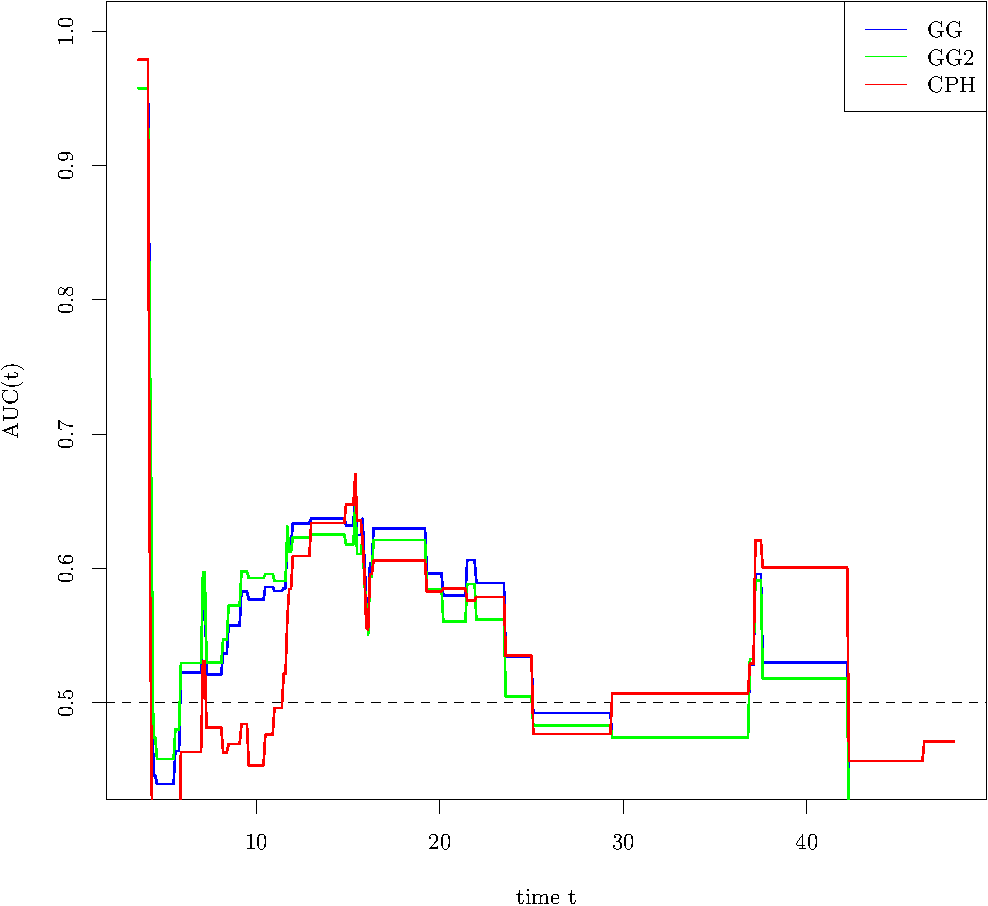
\includegraphics[width=\maxwidth]{figure/05-model-selection-auc-1} 

}



\end{knitrout}


Decision curve analysis.
\begin{knitrout}
\definecolor{shadecolor}{rgb}{0.969, 0.969, 0.969}\color{fgcolor}\begin{kframe}
\begin{alltt}
\hlstd{temp.data} \hlkwb{=} \hlkwd{data.frame}\hlstd{(}\hlkwc{Time} \hlstd{= data.val}\hlopt{$}\hlstd{Time,} \hlkwc{DSD} \hlstd{= data.val}\hlopt{$}\hlstd{DSD}\hlopt{*}\hlnum{1}\hlstd{,}
    \hlkwc{gg.1} \hlstd{=} \hlnum{1}\hlopt{-}\hlstd{val.prob.gg[val.prob.times} \hlopt{==} \hlnum{365}\hlstd{,],} \hlkwc{gg.2} \hlstd{=} \hlnum{1}\hlopt{-}\hlstd{val.prob.gg[val.prob.times} \hlopt{==} \hlnum{365}\hlopt{*}\hlnum{2}\hlstd{,],} \hlkwc{gg.3} \hlstd{=} \hlnum{1}\hlopt{-}\hlstd{val.prob.gg[val.prob.times} \hlopt{==} \hlnum{365}\hlopt{*}\hlnum{3}\hlstd{,],}
    \hlkwc{gg2.1} \hlstd{=} \hlnum{1}\hlopt{-}\hlstd{val.prob.gg2[val.prob.times} \hlopt{==} \hlnum{365}\hlstd{,],} \hlkwc{gg2.2} \hlstd{=} \hlnum{1}\hlopt{-}\hlstd{val.prob.gg2[val.prob.times} \hlopt{==} \hlnum{365}\hlopt{*}\hlnum{2}\hlstd{,],} \hlkwc{gg2.3} \hlstd{=} \hlnum{1}\hlopt{-}\hlstd{val.prob.gg2[val.prob.times} \hlopt{==} \hlnum{365}\hlopt{*}\hlnum{3}\hlstd{,],}
    \hlkwc{cph.1} \hlstd{=} \hlnum{1}\hlopt{-}\hlstd{val.prob.cph[val.prob.times} \hlopt{==} \hlnum{365}\hlstd{,],} \hlkwc{cph.2} \hlstd{=} \hlnum{1}\hlopt{-}\hlstd{val.prob.cph[val.prob.times} \hlopt{==} \hlnum{365}\hlopt{*}\hlnum{2}\hlstd{,],} \hlkwc{cph.3} \hlstd{=} \hlnum{1}\hlopt{-}\hlstd{val.prob.cph[val.prob.times} \hlopt{==} \hlnum{365}\hlopt{*}\hlnum{3}\hlstd{,],}
    \hlkwc{rsf.1} \hlstd{=} \hlnum{1}\hlopt{-}\hlstd{val.prob.rsf[val.prob.times} \hlopt{==} \hlnum{365}\hlstd{,],} \hlkwc{rsf.2} \hlstd{=} \hlnum{1}\hlopt{-}\hlstd{val.prob.rsf[val.prob.times} \hlopt{==} \hlnum{365}\hlopt{*}\hlnum{2}\hlstd{,],} \hlkwc{rsf.3} \hlstd{=} \hlnum{1}\hlopt{-}\hlstd{val.prob.rsf[val.prob.times} \hlopt{==} \hlnum{365}\hlopt{*}\hlnum{3}\hlstd{,])}
\hlkwd{stdca}\hlstd{(}\hlkwc{data} \hlstd{= temp.data,} \hlkwc{outcome} \hlstd{=} \hlstr{"DSD"}\hlstd{,} \hlkwc{ttoutcome} \hlstd{=} \hlstr{"Time"}\hlstd{,} \hlkwc{predictors} \hlstd{=} \hlkwd{c}\hlstd{(}\hlstr{"gg.1"}\hlstd{,} \hlstr{"cph.1"}\hlstd{,} \hlstr{"rsf.1"}\hlstd{),} \hlkwc{timepoint} \hlstd{=} \hlnum{365}\hlstd{,} \hlkwc{probability} \hlstd{=} \hlkwd{rep}\hlstd{(}\hlnum{TRUE}\hlstd{,} \hlnum{3}\hlstd{))}
\end{alltt}


{\ttfamily\noindent\bfseries\color{errorcolor}{\#\# Error in eval(expr, envir, enclos): could not find function "{}stdca"{}}}\begin{alltt}
\hlkwd{stdca}\hlstd{(}\hlkwc{data} \hlstd{= temp.data,} \hlkwc{outcome} \hlstd{=} \hlstr{"DSD"}\hlstd{,} \hlkwc{ttoutcome} \hlstd{=} \hlstr{"Time"}\hlstd{,} \hlkwc{predictors} \hlstd{=} \hlkwd{c}\hlstd{(}\hlstr{"gg.2"}\hlstd{,} \hlstr{"cph.2"}\hlstd{,} \hlstr{"rsf.2"}\hlstd{),} \hlkwc{timepoint} \hlstd{=} \hlnum{365}\hlopt{*}\hlnum{2}\hlstd{,} \hlkwc{probability} \hlstd{=} \hlkwd{rep}\hlstd{(}\hlnum{TRUE}\hlstd{,} \hlnum{3}\hlstd{))}
\end{alltt}


{\ttfamily\noindent\bfseries\color{errorcolor}{\#\# Error in eval(expr, envir, enclos): could not find function "{}stdca"{}}}\begin{alltt}
\hlkwd{stdca}\hlstd{(}\hlkwc{data} \hlstd{= temp.data,} \hlkwc{outcome} \hlstd{=} \hlstr{"DSD"}\hlstd{,} \hlkwc{ttoutcome} \hlstd{=} \hlstr{"Time"}\hlstd{,} \hlkwc{predictors} \hlstd{=} \hlkwd{c}\hlstd{(}\hlstr{"gg.3"}\hlstd{,} \hlstr{"cph.3"}\hlstd{,} \hlstr{"rsf.3"}\hlstd{),} \hlkwc{timepoint} \hlstd{=} \hlnum{365}\hlopt{*}\hlnum{3}\hlstd{,} \hlkwc{probability} \hlstd{=} \hlkwd{rep}\hlstd{(}\hlnum{TRUE}\hlstd{,} \hlnum{3}\hlstd{))}
\end{alltt}


{\ttfamily\noindent\bfseries\color{errorcolor}{\#\# Error in eval(expr, envir, enclos): could not find function "{}stdca"{}}}\end{kframe}
\end{knitrout}


Evaluate IBS point estimates.
BS paths over time on bootstrap samples of the holdout set.
\begin{knitrout}
\definecolor{shadecolor}{rgb}{0.969, 0.969, 0.969}\color{fgcolor}\begin{kframe}
\begin{alltt}
\hlkwd{set.seed}\hlstd{(}\hlnum{20150111}\hlstd{)}
\hlstd{ibs_eval_times} \hlkwb{=} \hlkwd{calcIBS}\hlstd{(}\hlkwd{Surv}\hlstd{(data.val}\hlopt{$}\hlstd{Time, data.val}\hlopt{$}\hlstd{DSD), ibs_preds_gg, ibs_times,} \hlkwd{max}\hlstd{(data.val}\hlopt{$}\hlstd{Time))}\hlopt{$}\hlstd{eval_times}
\hlcom{# bsc_boot2 = lapply(ibs_preds_all, function(preds) boot(data.val, statistic = function(d, i) calcIBS(Surv(d$Time, d$DSD)[i,], preds[i,], ibs_times, max(d$Time))$bsc, R = 500))}
\hlcom{# bsc_boot2ci = lapply(bsc_boot2, function(single_boot) t(sapply(1:length(ibs_eval_times), function(time_index) \{}
\hlcom{# 	temp = try(boot.ci(single_boot, index = time_index, type = "bca")$bca, silent = TRUE)}
\hlcom{# 	if (class(temp) == "try-error" || is.null(temp)) \{ temp = rep(NA, 5) \}}
\hlcom{# 	temp \})))}
\hlstd{bsc_boots} \hlkwb{=} \hlkwd{laply}\hlstd{(}\hlnum{1}\hlopt{:}\hlnum{500}\hlstd{,} \hlkwa{function}\hlstd{(}\hlkwc{i}\hlstd{) \{}
        \hlkwa{if} \hlstd{(i} \hlopt \hlnum{50} \hlopt{==} \hlnum{0}\hlstd{)       \{} \hlkwd{message}\hlstd{(i) \}}
        \hlstd{boot_samp} \hlkwb{=} \hlkwd{sample.int}\hlstd{(}\hlkwd{nrow}\hlstd{(data.val),} \hlkwc{replace} \hlstd{=} \hlnum{TRUE}\hlstd{)}
        \hlstd{gg} \hlkwb{=} \hlkwd{calcIBS}\hlstd{(}\hlkwd{Surv}\hlstd{(data.val}\hlopt{$}\hlstd{Time, data.val}\hlopt{$}\hlstd{DSD)[boot_samp,], ibs_preds_gg[boot_samp,], ibs_times,} \hlkwd{max}\hlstd{(data.val}\hlopt{$}\hlstd{Time))}\hlopt{$}\hlstd{bsc}
        \hlstd{gg2} \hlkwb{=} \hlkwd{calcIBS}\hlstd{(}\hlkwd{Surv}\hlstd{(data.val}\hlopt{$}\hlstd{Time, data.val}\hlopt{$}\hlstd{DSD)[boot_samp,], ibs_preds_gg2[boot_samp,], ibs_times,} \hlkwd{max}\hlstd{(data.val}\hlopt{$}\hlstd{Time))}\hlopt{$}\hlstd{bsc}
        \hlstd{cph} \hlkwb{=} \hlkwd{calcIBS}\hlstd{(}\hlkwd{Surv}\hlstd{(data.val}\hlopt{$}\hlstd{Time, data.val}\hlopt{$}\hlstd{DSD)[boot_samp,], ibs_preds_cph[boot_samp,], ibs_times,} \hlkwd{max}\hlstd{(data.val}\hlopt{$}\hlstd{Time))}\hlopt{$}\hlstd{bsc}
        \hlstd{rsf} \hlkwb{=} \hlkwd{calcIBS}\hlstd{(}\hlkwd{Surv}\hlstd{(data.val}\hlopt{$}\hlstd{Time, data.val}\hlopt{$}\hlstd{DSD)[boot_samp,], ibs_preds_rsf[boot_samp,], ibs_times,} \hlkwd{max}\hlstd{(data.val}\hlopt{$}\hlstd{Time))}\hlopt{$}\hlstd{bsc}
        \hlstd{km0} \hlkwb{=} \hlkwd{calcIBS}\hlstd{(}\hlkwd{Surv}\hlstd{(data.val}\hlopt{$}\hlstd{Time, data.val}\hlopt{$}\hlstd{DSD)[boot_samp,], ibs_preds_km0[boot_samp,], ibs_times,} \hlkwd{max}\hlstd{(data.val}\hlopt{$}\hlstd{Time))}\hlopt{$}\hlstd{bsc}
        \hlkwd{rbind}\hlstd{(gg, gg2, cph, rsf, km0)}
\hlstd{\})}
\end{alltt}


{\ttfamily\noindent\itshape\color{messagecolor}{\#\# 50\\\#\# 100\\\#\# 150\\\#\# 200\\\#\# 250\\\#\# 300\\\#\# 350\\\#\# 400\\\#\# 450\\\#\# 500}}\end{kframe}
\end{knitrout}

\begin{knitrout}
\definecolor{shadecolor}{rgb}{0.969, 0.969, 0.969}\color{fgcolor}\begin{kframe}
\begin{alltt}
\hlstd{temp} \hlkwb{=} \hlkwd{sapply}\hlstd{(}\hlkwd{list}\hlstd{(}\hlkwc{gg} \hlstd{= ibs_preds_gg,} \hlkwc{gg2} \hlstd{= ibs_preds_gg2,} \hlkwc{cph} \hlstd{= ibs_preds_cph,} \hlkwc{rsf} \hlstd{= ibs_preds_rsf,} \hlkwc{km0} \hlstd{= ibs_preds_km0),} \hlkwa{function}\hlstd{(}\hlkwc{preds}\hlstd{)} \hlkwd{calcIBS}\hlstd{(}\hlkwd{Surv}\hlstd{(data.val}\hlopt{$}\hlstd{Time, data.val}\hlopt{$}\hlstd{DSD), preds, ibs_times,} \hlkwd{max}\hlstd{(data.val}\hlopt{$}\hlstd{Time))}\hlopt{$}\hlstd{bsc)}
\hlstd{temp} \hlkwb{=} \hlkwd{melt}\hlstd{(temp)}
\hlkwd{colnames}\hlstd{(temp)} \hlkwb{=} \hlkwd{c}\hlstd{(}\hlstr{"Time"}\hlstd{,} \hlstr{"Model"}\hlstd{,} \hlstr{"BS"}\hlstd{)}
\hlkwd{ggplot}\hlstd{(temp,} \hlkwd{aes}\hlstd{(}\hlkwc{x} \hlstd{= Time,} \hlkwc{y} \hlstd{= BS,} \hlkwc{colour} \hlstd{= Model))} \hlopt{+} \hlkwd{geom_line}\hlstd{()} \hlopt{+} \hlkwd{ylab}\hlstd{(}\hlstr{"Brier Score"}\hlstd{)} \hlopt{+} \hlkwd{geom_hline}\hlstd{(}\hlkwc{yintercept} \hlstd{=} \hlnum{0.25}\hlstd{)}
\end{alltt}
\end{kframe}

{\centering 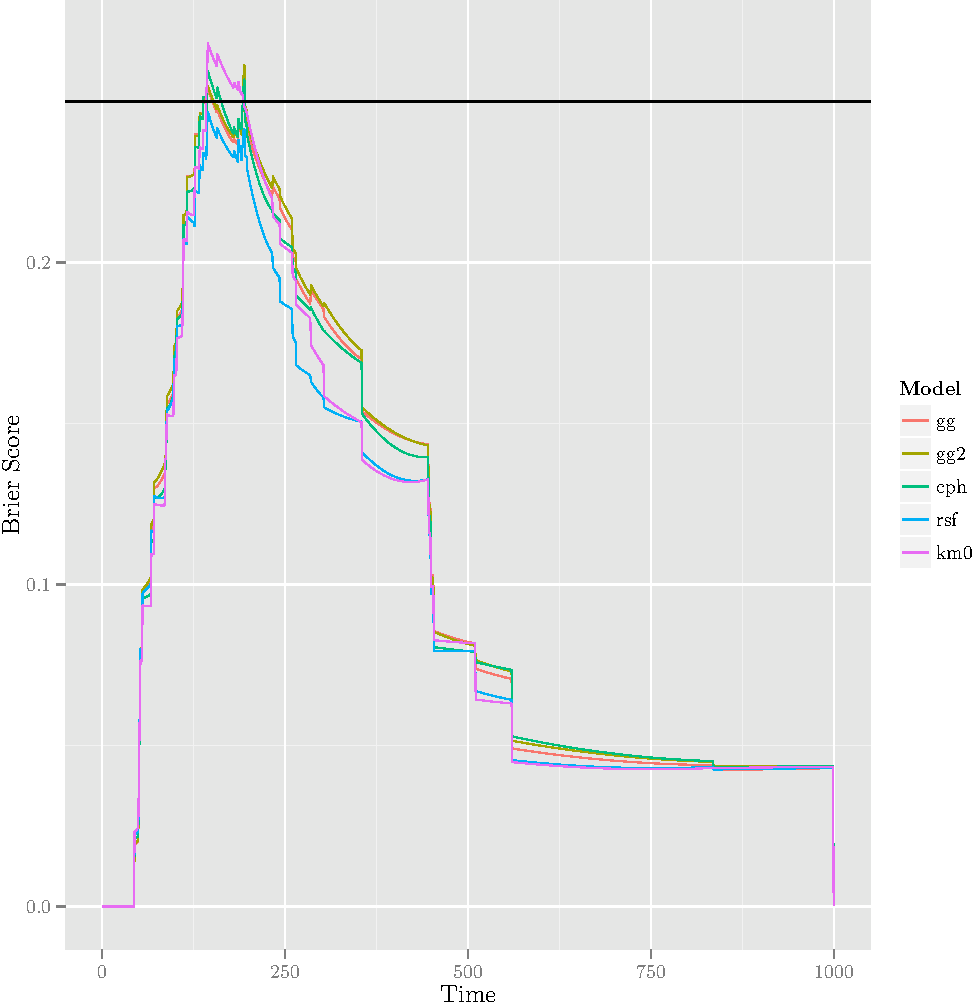
\includegraphics[width=\maxwidth]{figure/05-model-selection-bs-paths-1} 

}


\begin{kframe}\begin{alltt}
\hlstd{temp} \hlkwb{=} \hlkwd{melt}\hlstd{(}\hlkwd{aaply}\hlstd{(bsc_boots,} \hlnum{2}\hlopt{:}\hlnum{3}\hlstd{, quantile,} \hlkwc{probs} \hlstd{=} \hlkwd{c}\hlstd{(}\hlnum{0.05}\hlstd{,} \hlnum{0.5}\hlstd{,} \hlnum{0.95}\hlstd{)))}
\hlkwd{colnames}\hlstd{(temp)} \hlkwb{=} \hlkwd{c}\hlstd{(}\hlstr{"Model"}\hlstd{,} \hlstr{"Time"}\hlstd{,} \hlstr{"Quantile"}\hlstd{,} \hlstr{"Value"}\hlstd{)}
\hlstd{temp}\hlopt{$}\hlstd{Quantile} \hlkwb{=} \hlkwd{paste}\hlstd{(}\hlstr{"Q"}\hlstd{,} \hlkwd{gsub}\hlstd{(}\hlstr{"%"}\hlstd{,} \hlstr{""}\hlstd{, temp}\hlopt{$}\hlstd{Quantile),} \hlkwc{sep} \hlstd{=} \hlstr{""}\hlstd{)}
\hlstd{temp} \hlkwb{=} \hlkwd{dcast}\hlstd{(temp, Model} \hlopt{+} \hlstd{Time} \hlopt{~} \hlstd{Quantile,} \hlkwc{value.var} \hlstd{=} \hlstr{"Value"}\hlstd{)}
\hlkwd{ggplot}\hlstd{(temp,} \hlkwd{aes}\hlstd{(}\hlkwc{x} \hlstd{= Time,} \hlkwc{y} \hlstd{= Q50,} \hlkwc{ymin} \hlstd{= Q5,} \hlkwc{ymax} \hlstd{= Q95,} \hlkwc{colour} \hlstd{= Model,} \hlkwc{fill} \hlstd{= Model))} \hlopt{+} \hlkwd{geom_line}\hlstd{()} \hlopt{+} \hlkwd{geom_ribbon}\hlstd{(}\hlkwc{alpha} \hlstd{=} \hlnum{0.2}\hlstd{,} \hlkwc{colour} \hlstd{=} \hlnum{NA}\hlstd{)} \hlopt{+} \hlkwd{ylab}\hlstd{(}\hlstr{"Brier Score, 90\textbackslash{}\textbackslash{}% BI"}\hlstd{)} \hlopt{+} \hlkwd{geom_hline}\hlstd{(}\hlkwc{yintercept} \hlstd{=} \hlnum{0.25}\hlstd{)}
\end{alltt}
\end{kframe}

{\centering 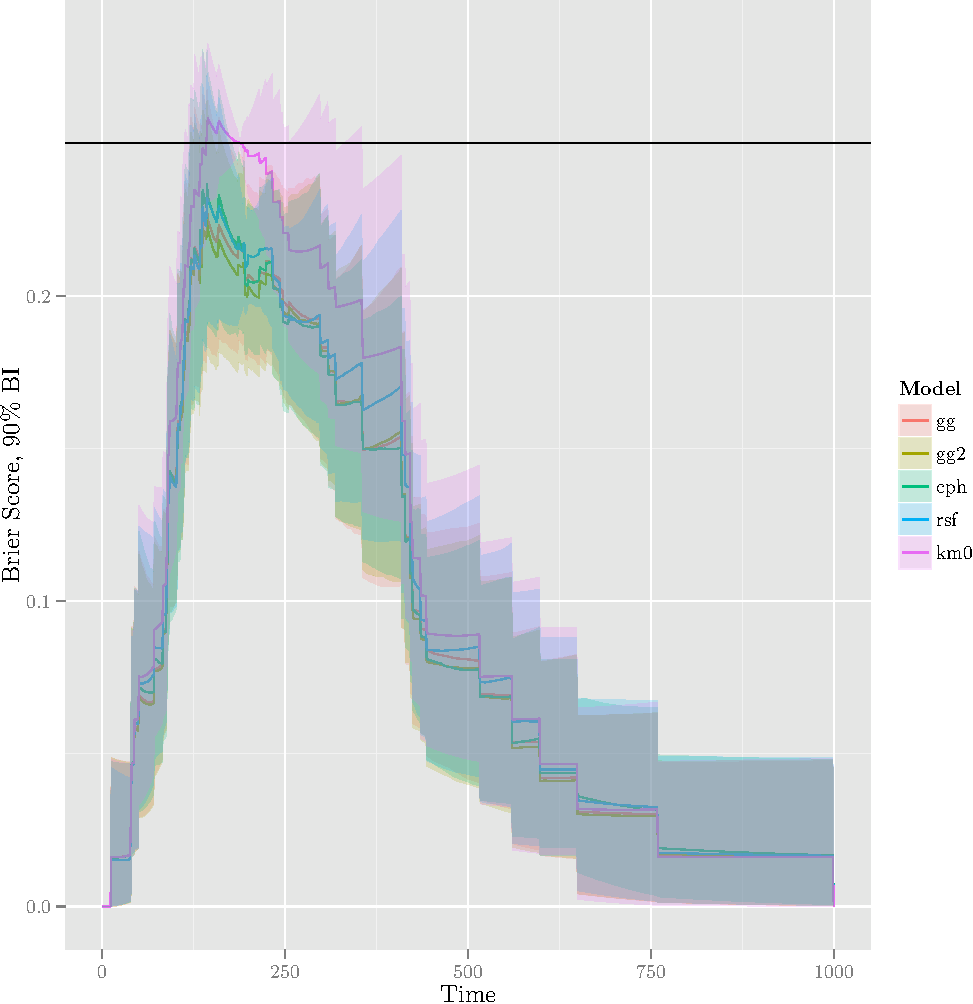
\includegraphics[width=\maxwidth]{figure/05-model-selection-bs-paths-2} 

}


\begin{kframe}\begin{alltt}
\hlstd{bsc_boots_diff} \hlkwb{=} \hlkwd{aaply}\hlstd{(bsc_boots,} \hlnum{2}\hlstd{,} \hlkwa{function}\hlstd{(}\hlkwc{x}\hlstd{) x} \hlopt{-} \hlstd{bsc_boots[,}\hlnum{5}\hlstd{,])[}\hlnum{1}\hlopt{:}\hlnum{4}\hlstd{,,]}
\hlstd{temp} \hlkwb{=} \hlkwd{melt}\hlstd{(}\hlkwd{aaply}\hlstd{(bsc_boots_diff,} \hlkwd{c}\hlstd{(}\hlnum{1}\hlstd{,}\hlnum{3}\hlstd{), quantile,} \hlkwc{probs} \hlstd{=} \hlkwd{c}\hlstd{(}\hlnum{0.05}\hlstd{,} \hlnum{0.5}\hlstd{,} \hlnum{0.95}\hlstd{)))}
\hlkwd{colnames}\hlstd{(temp)} \hlkwb{=} \hlkwd{c}\hlstd{(}\hlstr{"Model"}\hlstd{,} \hlstr{"Time"}\hlstd{,} \hlstr{"Quantile"}\hlstd{,} \hlstr{"Value"}\hlstd{)}
\hlstd{temp}\hlopt{$}\hlstd{Quantile} \hlkwb{=} \hlkwd{paste}\hlstd{(}\hlstr{"Q"}\hlstd{,} \hlkwd{gsub}\hlstd{(}\hlstr{"%"}\hlstd{,} \hlstr{""}\hlstd{, temp}\hlopt{$}\hlstd{Quantile),} \hlkwc{sep} \hlstd{=} \hlstr{""}\hlstd{)}
\hlstd{temp} \hlkwb{=} \hlkwd{dcast}\hlstd{(temp, Model} \hlopt{+} \hlstd{Time} \hlopt{~} \hlstd{Quantile,} \hlkwc{value.var} \hlstd{=} \hlstr{"Value"}\hlstd{)}
\hlkwd{ggplot}\hlstd{(temp,} \hlkwd{aes}\hlstd{(}\hlkwc{x} \hlstd{= Time,} \hlkwc{y} \hlstd{= Q50,} \hlkwc{ymin} \hlstd{= Q5,} \hlkwc{ymax} \hlstd{= Q95,} \hlkwc{colour} \hlstd{= Model,} \hlkwc{fill} \hlstd{= Model))} \hlopt{+} \hlkwd{geom_line}\hlstd{()} \hlopt{+} \hlkwd{geom_ribbon}\hlstd{(}\hlkwc{alpha} \hlstd{=} \hlnum{0.2}\hlstd{,} \hlkwc{colour} \hlstd{=} \hlnum{NA}\hlstd{)} \hlopt{+} \hlkwd{ylab}\hlstd{(}\hlstr{"Brier Score: Improvement over KM0. BS median, 90\textbackslash{}\textbackslash{}% BI"}\hlstd{)} \hlopt{+} \hlkwd{geom_hline}\hlstd{(}\hlkwc{yintercept} \hlstd{=} \hlnum{0}\hlstd{)}
\end{alltt}
\end{kframe}

{\centering 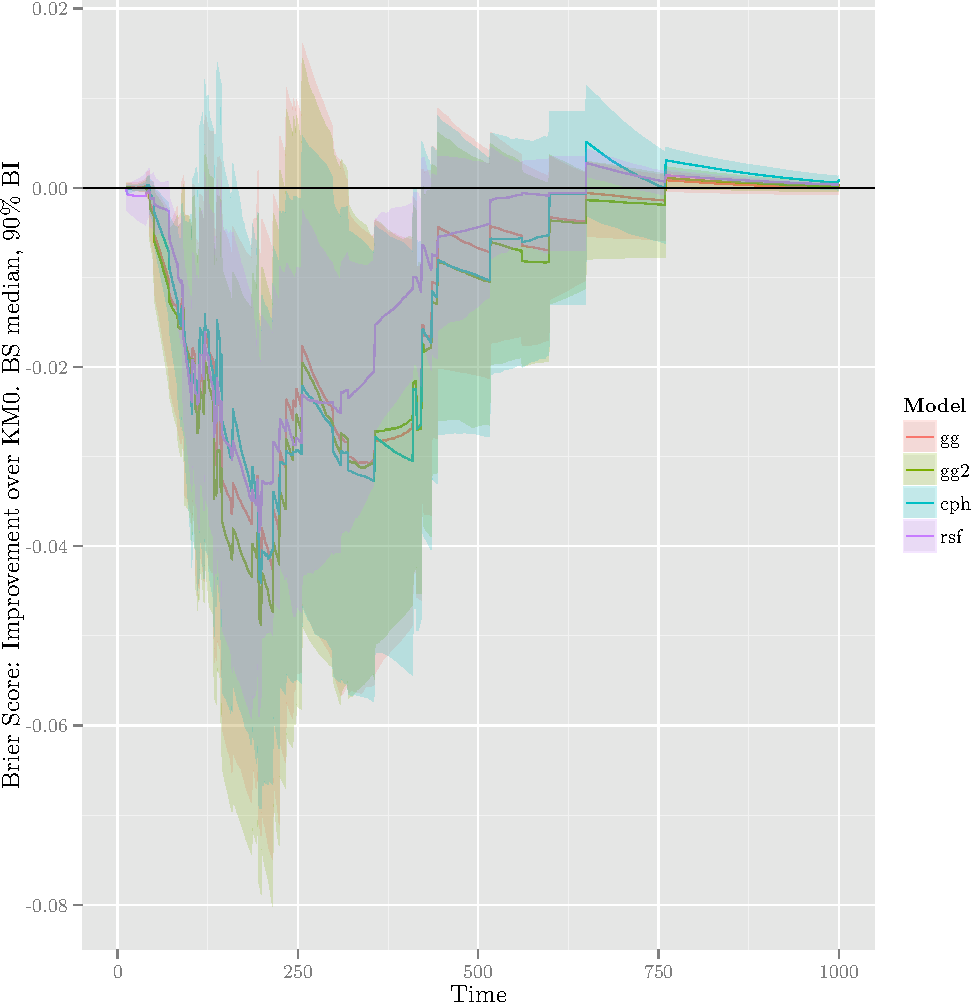
\includegraphics[width=\maxwidth]{figure/05-model-selection-bs-paths-3} 

}


\begin{kframe}\begin{alltt}
\hlkwd{ggplot}\hlstd{(temp,} \hlkwd{aes}\hlstd{(}\hlkwc{x} \hlstd{= Time,} \hlkwc{y} \hlstd{= Q50,} \hlkwc{ymin} \hlstd{= Q5,} \hlkwc{ymax} \hlstd{= Q95,} \hlkwc{colour} \hlstd{= Model,} \hlkwc{fill} \hlstd{= Model))} \hlopt{+} \hlkwd{geom_line}\hlstd{()} \hlopt{+} \hlkwd{geom_ribbon}\hlstd{(}\hlkwc{alpha} \hlstd{=} \hlnum{0.2}\hlstd{,} \hlkwc{colour} \hlstd{=} \hlnum{NA}\hlstd{)} \hlopt{+} \hlkwd{xlim}\hlstd{(}\hlnum{0}\hlstd{,} \hlnum{700}\hlstd{)} \hlopt{+} \hlkwd{ylab}\hlstd{(}\hlstr{"Brier Score: Improvement over KM0. BS median, 90\textbackslash{}\textbackslash{}% BI"}\hlstd{)} \hlopt{+} \hlkwd{geom_hline}\hlstd{(}\hlkwc{yintercept} \hlstd{=} \hlnum{0}\hlstd{)}
\end{alltt}


{\ttfamily\noindent\color{warningcolor}{\#\# Warning: Removed 1200 rows containing missing values (geom\_path).}}\end{kframe}

{\centering 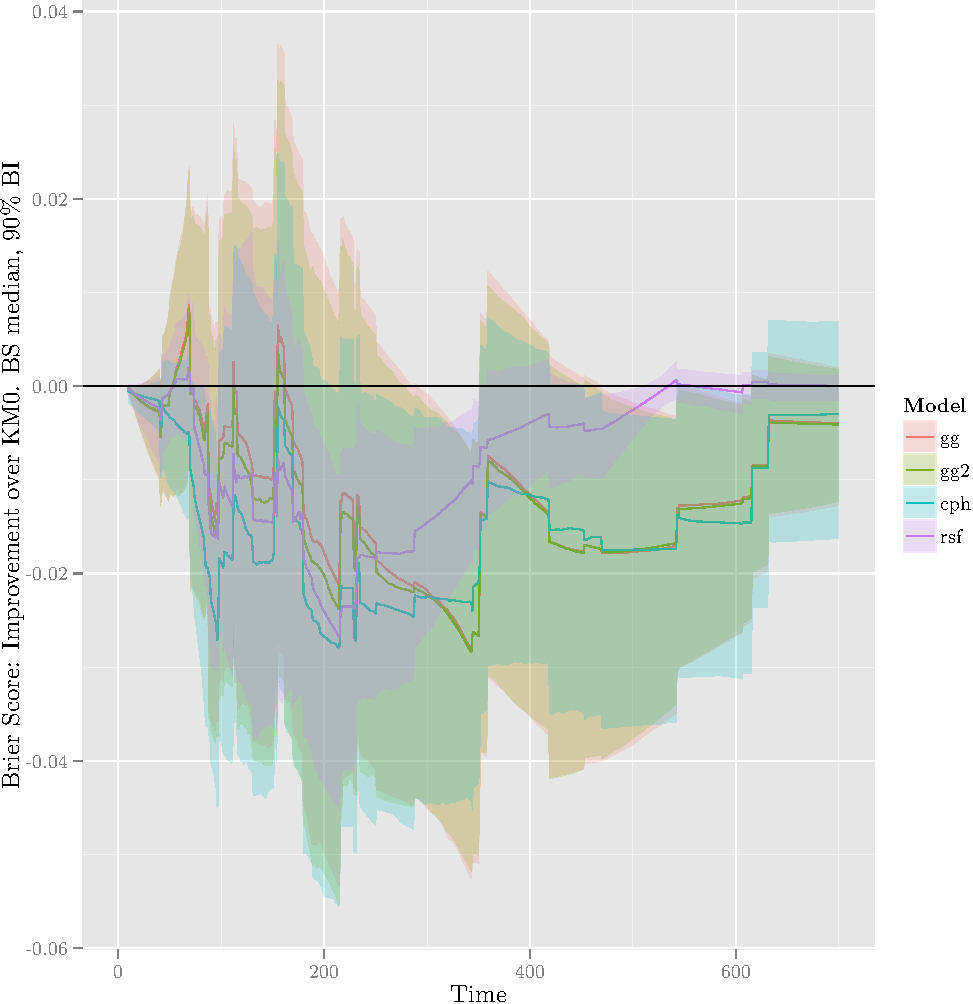
\includegraphics[width=\maxwidth]{figure/05-model-selection-bs-paths-4} 

}


\begin{kframe}\begin{alltt}
\hlkwd{ggplot}\hlstd{(temp,} \hlkwd{aes}\hlstd{(}\hlkwc{x} \hlstd{= Time,} \hlkwc{y} \hlstd{= Q50,} \hlkwc{colour} \hlstd{= Model))} \hlopt{+} \hlkwd{geom_line}\hlstd{()} \hlopt{+} \hlkwd{ylab}\hlstd{(}\hlstr{"Brier Score: Improvement over KM0, BS median"}\hlstd{)} \hlopt{+} \hlkwd{geom_hline}\hlstd{(}\hlkwc{yintercept} \hlstd{=} \hlnum{0}\hlstd{)}
\end{alltt}
\end{kframe}

{\centering 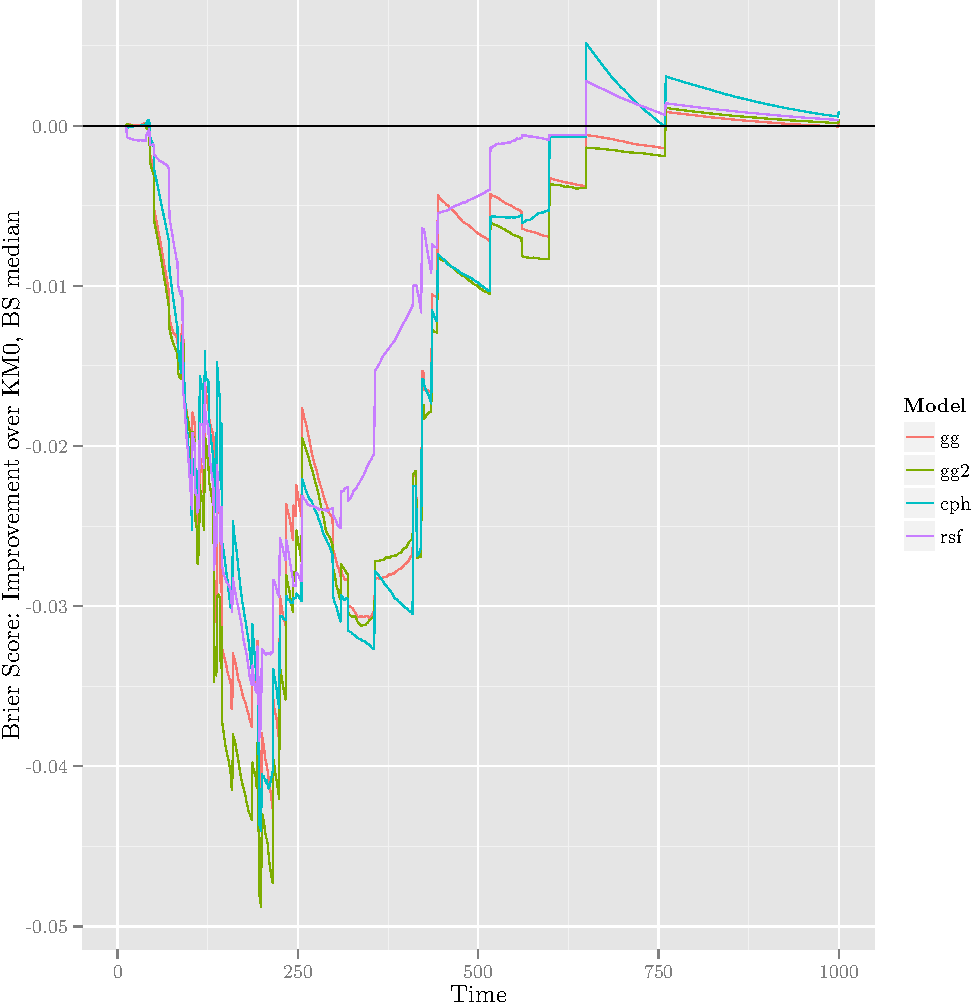
\includegraphics[width=\maxwidth]{figure/05-model-selection-bs-paths-5} 

}


\begin{kframe}\begin{alltt}
\hlkwd{ggplot}\hlstd{(temp,} \hlkwd{aes}\hlstd{(}\hlkwc{x} \hlstd{= Time,} \hlkwc{y} \hlstd{= Q50,} \hlkwc{colour} \hlstd{= Model))} \hlopt{+} \hlkwd{geom_line}\hlstd{()} \hlopt{+} \hlkwd{ylab}\hlstd{(}\hlstr{"Brier Score: Improvement over KM0, BS median"}\hlstd{)} \hlopt{+} \hlkwd{xlim}\hlstd{(}\hlnum{0}\hlstd{,} \hlnum{700}\hlstd{)} \hlopt{+} \hlkwd{geom_hline}\hlstd{(}\hlkwc{yintercept} \hlstd{=} \hlnum{0}\hlstd{)}
\end{alltt}


{\ttfamily\noindent\color{warningcolor}{\#\# Warning: Removed 1200 rows containing missing values (geom\_path).}}\end{kframe}

{\centering 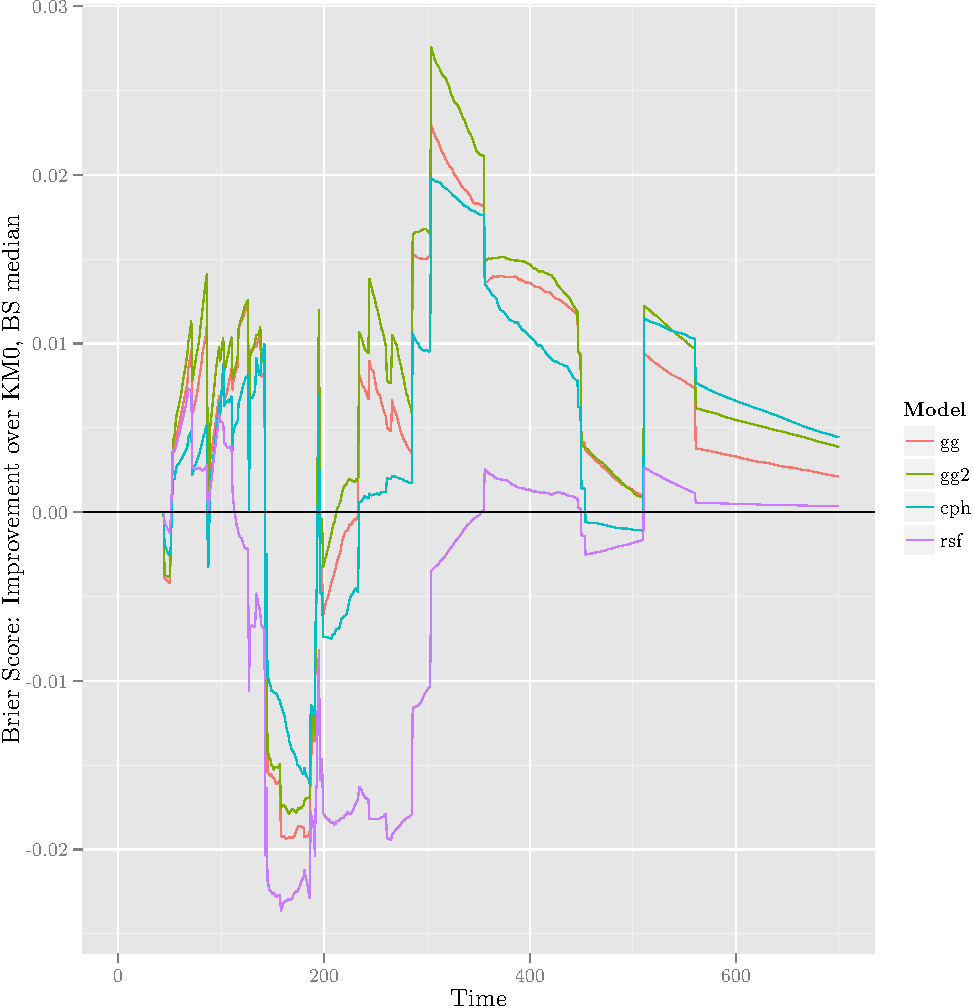
\includegraphics[width=\maxwidth]{figure/05-model-selection-bs-paths-6} 

}



\end{knitrout}

IBS comparisons.
\begin{knitrout}
\definecolor{shadecolor}{rgb}{0.969, 0.969, 0.969}\color{fgcolor}\begin{kframe}
\begin{alltt}
\hlkwd{set.seed}\hlstd{(}\hlnum{20150111}\hlstd{)}
\hlstd{ibsc_boots} \hlkwb{=} \hlkwd{t}\hlstd{(}\hlkwd{sapply}\hlstd{(}\hlnum{1}\hlopt{:}\hlnum{5e2}\hlstd{,} \hlkwa{function}\hlstd{(}\hlkwc{i}\hlstd{) \{}
        \hlkwa{if} \hlstd{(i} \hlopt \hlnum{5e1} \hlopt{==} \hlnum{0}\hlstd{)      \{} \hlkwd{message}\hlstd{(i) \}}
        \hlstd{boot_samp} \hlkwb{=} \hlkwd{sample.int}\hlstd{(}\hlkwd{nrow}\hlstd{(data.val),} \hlkwc{replace} \hlstd{=} \hlnum{TRUE}\hlstd{)}
        \hlstd{gg} \hlkwb{=} \hlkwd{calcIBS}\hlstd{(}\hlkwd{Surv}\hlstd{(data.val}\hlopt{$}\hlstd{Time, data.val}\hlopt{$}\hlstd{DSD)[boot_samp,], ibs_preds_gg[boot_samp,], ibs_times,} \hlkwd{max}\hlstd{(data.val}\hlopt{$}\hlstd{Time[boot_samp]))}\hlopt{$}\hlstd{ibs}
        \hlstd{gg2} \hlkwb{=} \hlkwd{calcIBS}\hlstd{(}\hlkwd{Surv}\hlstd{(data.val}\hlopt{$}\hlstd{Time, data.val}\hlopt{$}\hlstd{DSD)[boot_samp,], ibs_preds_gg2[boot_samp,], ibs_times,} \hlkwd{max}\hlstd{(data.val}\hlopt{$}\hlstd{Time[boot_samp]))}\hlopt{$}\hlstd{ibs}
        \hlstd{cph} \hlkwb{=} \hlkwd{calcIBS}\hlstd{(}\hlkwd{Surv}\hlstd{(data.val}\hlopt{$}\hlstd{Time, data.val}\hlopt{$}\hlstd{DSD)[boot_samp,], ibs_preds_cph[boot_samp,], ibs_times,} \hlkwd{max}\hlstd{(data.val}\hlopt{$}\hlstd{Time[boot_samp]))}\hlopt{$}\hlstd{ibs}
        \hlstd{rsf} \hlkwb{=} \hlkwd{calcIBS}\hlstd{(}\hlkwd{Surv}\hlstd{(data.val}\hlopt{$}\hlstd{Time, data.val}\hlopt{$}\hlstd{DSD)[boot_samp,], ibs_preds_rsf[boot_samp,], ibs_times,} \hlkwd{max}\hlstd{(data.val}\hlopt{$}\hlstd{Time[boot_samp]))}\hlopt{$}\hlstd{ibs}
        \hlstd{km0} \hlkwb{=} \hlkwd{calcIBS}\hlstd{(}\hlkwd{Surv}\hlstd{(data.val}\hlopt{$}\hlstd{Time, data.val}\hlopt{$}\hlstd{DSD)[boot_samp,], ibs_preds_km0[boot_samp,], ibs_times,} \hlkwd{max}\hlstd{(data.val}\hlopt{$}\hlstd{Time[boot_samp]))}\hlopt{$}\hlstd{ibs}
        \hlkwd{c}\hlstd{(gg, gg2, cph, rsf, km0)}
\hlstd{\}))}
\end{alltt}


{\ttfamily\noindent\itshape\color{messagecolor}{\#\# 50\\\#\# 100\\\#\# 150\\\#\# 200\\\#\# 250\\\#\# 300\\\#\# 350\\\#\# 400\\\#\# 450\\\#\# 500}}\begin{alltt}
\hlkwd{colnames}\hlstd{(ibsc_boots)} \hlkwb{=} \hlkwd{c}\hlstd{(}\hlstr{"gg"}\hlstd{,} \hlstr{"gg2"}\hlstd{,} \hlstr{"cph"}\hlstd{,} \hlstr{"rsf"}\hlstd{,} \hlstr{"km0"}\hlstd{)}
\end{alltt}
\end{kframe}
\end{knitrout}

\begin{knitrout}
\definecolor{shadecolor}{rgb}{0.969, 0.969, 0.969}\color{fgcolor}\begin{kframe}
\begin{alltt}
\hlkwd{calcIBS}\hlstd{(}\hlkwd{Surv}\hlstd{(data.val}\hlopt{$}\hlstd{Time, data.val}\hlopt{$}\hlstd{DSD), ibs_preds_gg, ibs_times,} \hlkwd{max}\hlstd{(data.val}\hlopt{$}\hlstd{Time))}\hlopt{$}\hlstd{ibs}
\end{alltt}
\begin{verbatim}
## [1] 229.8
\end{verbatim}
\begin{alltt}
\hlkwd{calcIBS}\hlstd{(}\hlkwd{Surv}\hlstd{(data.val}\hlopt{$}\hlstd{Time, data.val}\hlopt{$}\hlstd{DSD), ibs_preds_gg2, ibs_times,} \hlkwd{max}\hlstd{(data.val}\hlopt{$}\hlstd{Time))}\hlopt{$}\hlstd{ibs}
\end{alltt}
\begin{verbatim}
## [1] 228.9
\end{verbatim}
\begin{alltt}
\hlkwd{calcIBS}\hlstd{(}\hlkwd{Surv}\hlstd{(data.val}\hlopt{$}\hlstd{Time, data.val}\hlopt{$}\hlstd{DSD), ibs_preds_cph, ibs_times,} \hlkwd{max}\hlstd{(data.val}\hlopt{$}\hlstd{Time))}\hlopt{$}\hlstd{ibs}
\end{alltt}
\begin{verbatim}
## [1] 229.2
\end{verbatim}
\begin{alltt}
\hlkwd{calcIBS}\hlstd{(}\hlkwd{Surv}\hlstd{(data.val}\hlopt{$}\hlstd{Time, data.val}\hlopt{$}\hlstd{DSD), ibs_preds_rsf, ibs_times,} \hlkwd{max}\hlstd{(data.val}\hlopt{$}\hlstd{Time))}\hlopt{$}\hlstd{ibs}
\end{alltt}
\begin{verbatim}
## [1] 244.3
\end{verbatim}
\begin{alltt}
\hlkwd{calcIBS}\hlstd{(}\hlkwd{Surv}\hlstd{(data.val}\hlopt{$}\hlstd{Time, data.val}\hlopt{$}\hlstd{DSD), ibs_preds_km0, ibs_times,} \hlkwd{max}\hlstd{(data.val}\hlopt{$}\hlstd{Time))}\hlopt{$}\hlstd{ibs}
\end{alltt}
\begin{verbatim}
## [1] 254.1
\end{verbatim}
\begin{alltt}
\hlkwd{boxplot}\hlstd{(ibsc_boots,} \hlkwc{main} \hlstd{=} \hlstr{"IBS BS Distribution"}\hlstd{,} \hlkwc{ylab} \hlstd{=} \hlstr{"IBS"}\hlstd{)}
\end{alltt}
\end{kframe}

{\centering 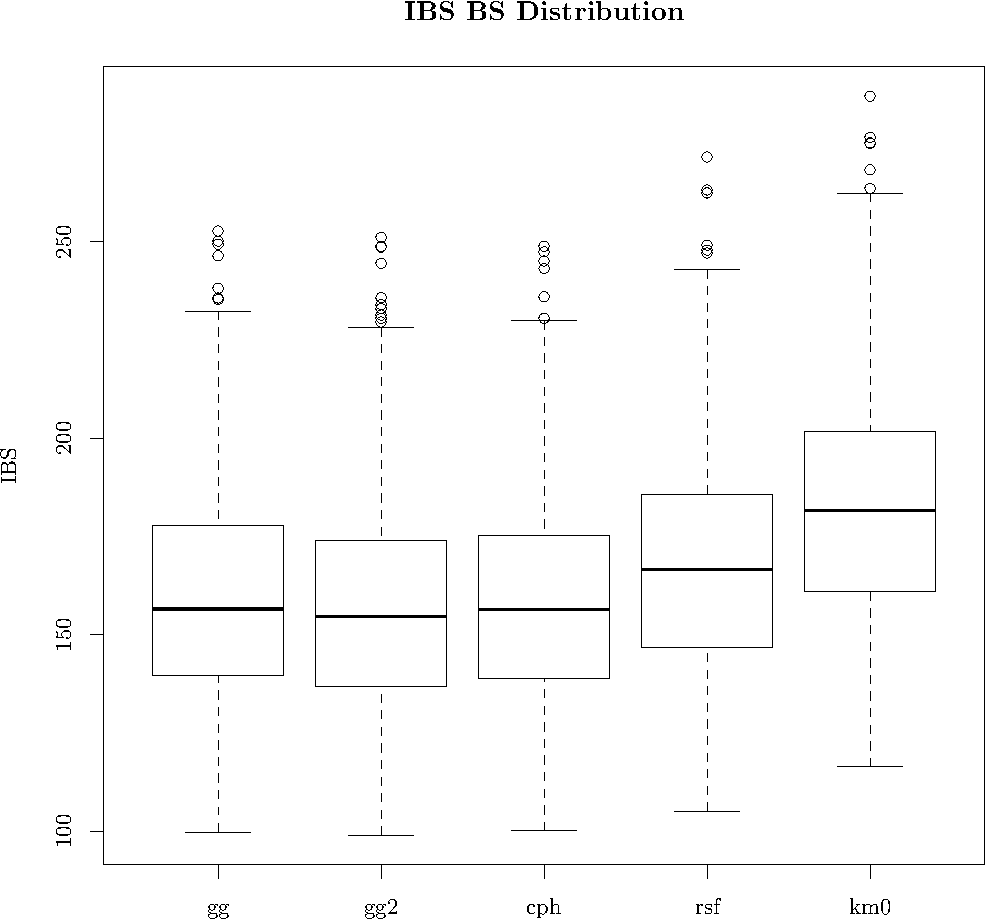
\includegraphics[width=\maxwidth]{figure/05-model-selection-ibs-1} 

}


\begin{kframe}\begin{alltt}
\hlkwd{plot}\hlstd{(}\hlkwd{density}\hlstd{(ibsc_boots[,}\hlnum{1}\hlstd{]),} \hlkwc{col} \hlstd{=} \hlstr{"blue"}\hlstd{,} \hlkwc{lwd} \hlstd{=} \hlnum{2}\hlstd{,} \hlkwc{main} \hlstd{=} \hlstr{"IBS BS Distribution"}\hlstd{,} \hlkwc{xlab} \hlstd{=} \hlstr{"IBS"}\hlstd{)}
\hlkwd{lines}\hlstd{(}\hlkwd{density}\hlstd{(ibsc_boots[,}\hlnum{2}\hlstd{]),} \hlkwc{col} \hlstd{=} \hlstr{"red"}\hlstd{,} \hlkwc{lwd} \hlstd{=} \hlnum{2}\hlstd{)}
\hlkwd{lines}\hlstd{(}\hlkwd{density}\hlstd{(ibsc_boots[,}\hlnum{3}\hlstd{]),} \hlkwc{col} \hlstd{=} \hlstr{"green"}\hlstd{,} \hlkwc{lwd} \hlstd{=} \hlnum{2}\hlstd{)}
\hlkwd{lines}\hlstd{(}\hlkwd{density}\hlstd{(ibsc_boots[,}\hlnum{4}\hlstd{]),} \hlkwc{col} \hlstd{=} \hlstr{"purple"}\hlstd{,} \hlkwc{lwd} \hlstd{=} \hlnum{2}\hlstd{)}
\hlkwd{lines}\hlstd{(}\hlkwd{density}\hlstd{(ibsc_boots[,}\hlnum{5}\hlstd{]),} \hlkwc{col} \hlstd{=} \hlstr{"black"}\hlstd{,} \hlkwc{lwd} \hlstd{=} \hlnum{2}\hlstd{)}
\hlkwd{abline}\hlstd{(}\hlkwc{v} \hlstd{=} \hlkwd{calcIBS}\hlstd{(}\hlkwd{Surv}\hlstd{(data.val}\hlopt{$}\hlstd{Time, data.val}\hlopt{$}\hlstd{DSD), ibs_preds_gg, ibs_times,} \hlkwd{max}\hlstd{(data.val}\hlopt{$}\hlstd{Time))}\hlopt{$}\hlstd{ibs,} \hlkwc{col} \hlstd{=} \hlstr{"blue"}\hlstd{,} \hlkwc{lwd} \hlstd{=} \hlnum{1}\hlstd{)}
\hlkwd{abline}\hlstd{(}\hlkwc{v} \hlstd{=} \hlkwd{calcIBS}\hlstd{(}\hlkwd{Surv}\hlstd{(data.val}\hlopt{$}\hlstd{Time, data.val}\hlopt{$}\hlstd{DSD), ibs_preds_gg2, ibs_times,} \hlkwd{max}\hlstd{(data.val}\hlopt{$}\hlstd{Time))}\hlopt{$}\hlstd{ibs,} \hlkwc{col} \hlstd{=} \hlstr{"red"}\hlstd{,} \hlkwc{lwd} \hlstd{=} \hlnum{1}\hlstd{)}
\hlkwd{abline}\hlstd{(}\hlkwc{v} \hlstd{=} \hlkwd{calcIBS}\hlstd{(}\hlkwd{Surv}\hlstd{(data.val}\hlopt{$}\hlstd{Time, data.val}\hlopt{$}\hlstd{DSD), ibs_preds_cph, ibs_times,} \hlkwd{max}\hlstd{(data.val}\hlopt{$}\hlstd{Time))}\hlopt{$}\hlstd{ibs,} \hlkwc{col} \hlstd{=} \hlstr{"green"}\hlstd{,} \hlkwc{lwd} \hlstd{=} \hlnum{1}\hlstd{)}
\hlkwd{abline}\hlstd{(}\hlkwc{v} \hlstd{=} \hlkwd{calcIBS}\hlstd{(}\hlkwd{Surv}\hlstd{(data.val}\hlopt{$}\hlstd{Time, data.val}\hlopt{$}\hlstd{DSD), ibs_preds_rsf, ibs_times,} \hlkwd{max}\hlstd{(data.val}\hlopt{$}\hlstd{Time))}\hlopt{$}\hlstd{ibs,} \hlkwc{col} \hlstd{=} \hlstr{"purple"}\hlstd{,} \hlkwc{lwd} \hlstd{=} \hlnum{1}\hlstd{)}
\hlkwd{abline}\hlstd{(}\hlkwc{v} \hlstd{=} \hlkwd{calcIBS}\hlstd{(}\hlkwd{Surv}\hlstd{(data.val}\hlopt{$}\hlstd{Time, data.val}\hlopt{$}\hlstd{DSD), ibs_preds_km0, ibs_times,} \hlkwd{max}\hlstd{(data.val}\hlopt{$}\hlstd{Time))}\hlopt{$}\hlstd{ibs,} \hlkwc{col} \hlstd{=} \hlstr{"black"}\hlstd{,} \hlkwc{lwd} \hlstd{=} \hlnum{1}\hlstd{)}
\hlkwd{legend}\hlstd{(}\hlstr{"topright"}\hlstd{,} \hlkwc{legend} \hlstd{=} \hlkwd{c}\hlstd{(}\hlstr{"gg"}\hlstd{,} \hlstr{"gg2"}\hlstd{,} \hlstr{"cph"}\hlstd{,} \hlstr{"rsf"}\hlstd{,} \hlstr{"km0"}\hlstd{),} \hlkwc{col} \hlstd{=} \hlkwd{c}\hlstd{(}\hlstr{"blue"}\hlstd{,} \hlstr{"red"}\hlstd{,} \hlstr{"green"}\hlstd{,} \hlstr{"purple"}\hlstd{,} \hlstr{"black"}\hlstd{),} \hlkwc{lty} \hlstd{=} \hlstr{"solid"}\hlstd{,} \hlkwc{inset} \hlstd{=} \hlnum{0.05}\hlstd{)}
\end{alltt}
\end{kframe}

{\centering 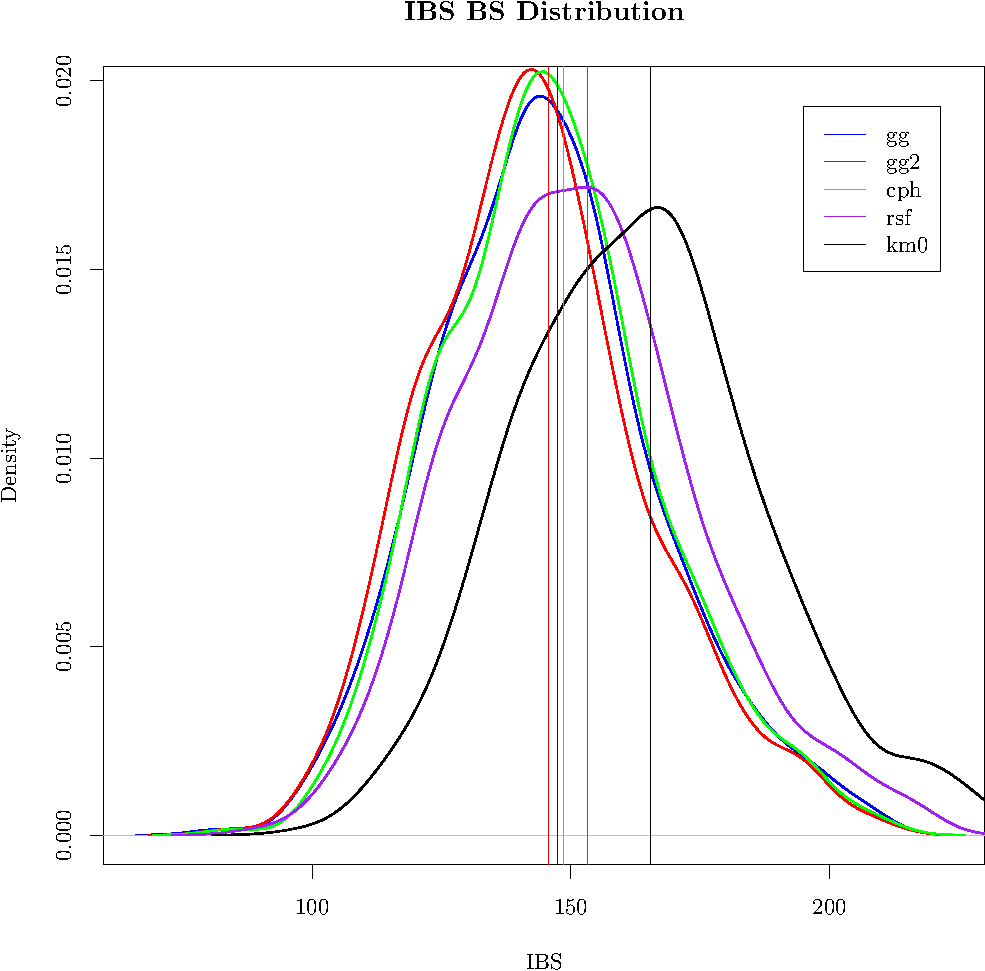
\includegraphics[width=\maxwidth]{figure/05-model-selection-ibs-2} 

}


\begin{kframe}\begin{alltt}
\hlkwd{plot}\hlstd{(}\hlkwd{density}\hlstd{(ibsc_boots[,}\hlnum{5}\hlstd{]} \hlopt{-} \hlstd{ibsc_boots[,}\hlnum{1}\hlstd{]),} \hlkwc{col} \hlstd{=} \hlstr{"blue"}\hlstd{,} \hlkwc{lwd} \hlstd{=} \hlnum{2}\hlstd{,} \hlkwc{main} \hlstd{=} \hlstr{"IBS\textbackslash{}\textbackslash{}_KM0 - IBS\textbackslash{}\textbackslash{}_x BS Distribution"}\hlstd{,} \hlkwc{xlab} \hlstd{=} \hlstr{"IBS"}\hlstd{,} \hlkwc{ylim} \hlstd{=} \hlkwd{c}\hlstd{(}\hlnum{0}\hlstd{,} \hlnum{0.1}\hlstd{))}
\hlkwd{lines}\hlstd{(}\hlkwd{density}\hlstd{(ibsc_boots[,}\hlnum{5}\hlstd{]} \hlopt{-} \hlstd{ibsc_boots[,}\hlnum{2}\hlstd{]),} \hlkwc{col} \hlstd{=} \hlstr{"red"}\hlstd{,} \hlkwc{lwd} \hlstd{=} \hlnum{2}\hlstd{)}
\hlkwd{lines}\hlstd{(}\hlkwd{density}\hlstd{(ibsc_boots[,}\hlnum{5}\hlstd{]} \hlopt{-} \hlstd{ibsc_boots[,}\hlnum{3}\hlstd{]),} \hlkwc{col} \hlstd{=} \hlstr{"green"}\hlstd{,} \hlkwc{lwd} \hlstd{=} \hlnum{2}\hlstd{)}
\hlkwd{lines}\hlstd{(}\hlkwd{density}\hlstd{(ibsc_boots[,}\hlnum{5}\hlstd{]} \hlopt{-} \hlstd{ibsc_boots[,}\hlnum{4}\hlstd{]),} \hlkwc{col} \hlstd{=} \hlstr{"purple"}\hlstd{,} \hlkwc{lwd} \hlstd{=} \hlnum{2}\hlstd{)}
\hlkwd{abline}\hlstd{(}\hlkwc{v} \hlstd{= (}\hlkwd{calcIBS}\hlstd{(}\hlkwd{Surv}\hlstd{(data.val}\hlopt{$}\hlstd{Time, data.val}\hlopt{$}\hlstd{DSD), ibs_preds_km0, ibs_times,} \hlkwd{max}\hlstd{(data.val}\hlopt{$}\hlstd{Time))}\hlopt{$}\hlstd{ibs} \hlopt{-} \hlkwd{calcIBS}\hlstd{(}\hlkwd{Surv}\hlstd{(data.val}\hlopt{$}\hlstd{Time, data.val}\hlopt{$}\hlstd{DSD), ibs_preds_gg, ibs_times,} \hlkwd{max}\hlstd{(data.val}\hlopt{$}\hlstd{Time))}\hlopt{$}\hlstd{ibs),} \hlkwc{col} \hlstd{=} \hlstr{"blue"}\hlstd{,} \hlkwc{lwd} \hlstd{=} \hlnum{1}\hlstd{)}
\hlkwd{abline}\hlstd{(}\hlkwc{v} \hlstd{= (}\hlkwd{calcIBS}\hlstd{(}\hlkwd{Surv}\hlstd{(data.val}\hlopt{$}\hlstd{Time, data.val}\hlopt{$}\hlstd{DSD), ibs_preds_km0, ibs_times,} \hlkwd{max}\hlstd{(data.val}\hlopt{$}\hlstd{Time))}\hlopt{$}\hlstd{ibs} \hlopt{-} \hlkwd{calcIBS}\hlstd{(}\hlkwd{Surv}\hlstd{(data.val}\hlopt{$}\hlstd{Time, data.val}\hlopt{$}\hlstd{DSD), ibs_preds_gg2, ibs_times,} \hlkwd{max}\hlstd{(data.val}\hlopt{$}\hlstd{Time))}\hlopt{$}\hlstd{ibs),} \hlkwc{col} \hlstd{=} \hlstr{"red"}\hlstd{,} \hlkwc{lwd} \hlstd{=} \hlnum{1}\hlstd{)}
\hlkwd{abline}\hlstd{(}\hlkwc{v} \hlstd{= (}\hlkwd{calcIBS}\hlstd{(}\hlkwd{Surv}\hlstd{(data.val}\hlopt{$}\hlstd{Time, data.val}\hlopt{$}\hlstd{DSD), ibs_preds_km0, ibs_times,} \hlkwd{max}\hlstd{(data.val}\hlopt{$}\hlstd{Time))}\hlopt{$}\hlstd{ibs} \hlopt{-} \hlkwd{calcIBS}\hlstd{(}\hlkwd{Surv}\hlstd{(data.val}\hlopt{$}\hlstd{Time, data.val}\hlopt{$}\hlstd{DSD), ibs_preds_cph, ibs_times,} \hlkwd{max}\hlstd{(data.val}\hlopt{$}\hlstd{Time))}\hlopt{$}\hlstd{ibs),} \hlkwc{col} \hlstd{=} \hlstr{"green"}\hlstd{,} \hlkwc{lwd} \hlstd{=} \hlnum{1}\hlstd{)}
\hlkwd{abline}\hlstd{(}\hlkwc{v} \hlstd{= (}\hlkwd{calcIBS}\hlstd{(}\hlkwd{Surv}\hlstd{(data.val}\hlopt{$}\hlstd{Time, data.val}\hlopt{$}\hlstd{DSD), ibs_preds_km0, ibs_times,} \hlkwd{max}\hlstd{(data.val}\hlopt{$}\hlstd{Time))}\hlopt{$}\hlstd{ibs} \hlopt{-} \hlkwd{calcIBS}\hlstd{(}\hlkwd{Surv}\hlstd{(data.val}\hlopt{$}\hlstd{Time, data.val}\hlopt{$}\hlstd{DSD), ibs_preds_rsf, ibs_times,} \hlkwd{max}\hlstd{(data.val}\hlopt{$}\hlstd{Time))}\hlopt{$}\hlstd{ibs),} \hlkwc{col} \hlstd{=} \hlstr{"purple"}\hlstd{,} \hlkwc{lwd} \hlstd{=} \hlnum{1}\hlstd{)}
\hlkwd{legend}\hlstd{(}\hlstr{"topright"}\hlstd{,} \hlkwc{legend} \hlstd{=} \hlkwd{c}\hlstd{(}\hlstr{"gg"}\hlstd{,} \hlstr{"gg2"}\hlstd{,} \hlstr{"cph"}\hlstd{,} \hlstr{"rsf"}\hlstd{),} \hlkwc{col} \hlstd{=} \hlkwd{c}\hlstd{(}\hlstr{"blue"}\hlstd{,} \hlstr{"red"}\hlstd{,} \hlstr{"green"}\hlstd{,} \hlstr{"purple"}\hlstd{),} \hlkwc{lty} \hlstd{=} \hlstr{"solid"}\hlstd{,} \hlkwc{inset} \hlstd{=} \hlnum{0.05}\hlstd{)}
\end{alltt}
\end{kframe}

{\centering 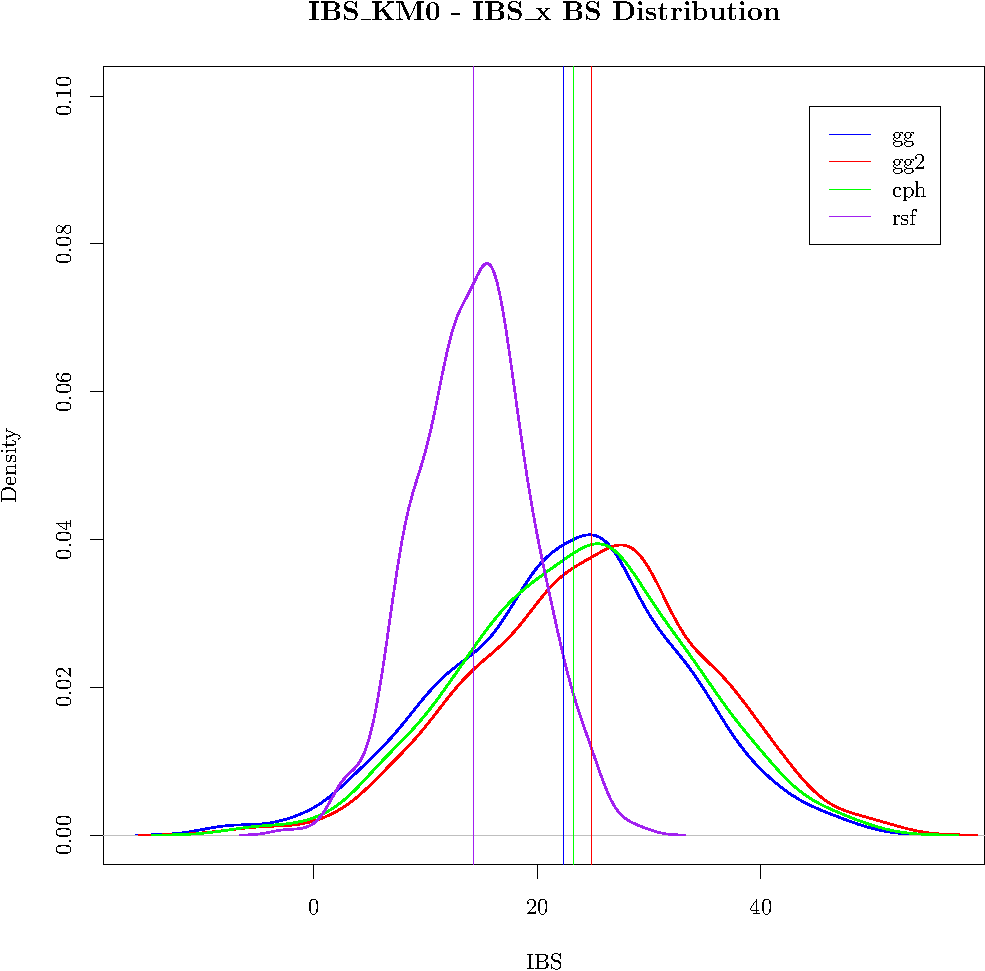
\includegraphics[width=\maxwidth]{figure/05-model-selection-ibs-3} 

}



\end{knitrout}

Do some proper BCA bootstrapping on the differences, just as a double-check test.
\begin{knitrout}
\definecolor{shadecolor}{rgb}{0.969, 0.969, 0.969}\color{fgcolor}\begin{kframe}
\begin{alltt}
\hlkwd{set.seed}\hlstd{(}\hlnum{20150111}\hlstd{)}
\hlstd{ibsc_boots2} \hlkwb{=} \hlkwd{boot}\hlstd{(data.val,} \hlkwc{statistic} \hlstd{=} \hlkwa{function}\hlstd{(}\hlkwc{d}\hlstd{,} \hlkwc{i}\hlstd{) \{}
        \hlstd{gg} \hlkwb{=} \hlkwd{calcIBS}\hlstd{(}\hlkwd{Surv}\hlstd{(d}\hlopt{$}\hlstd{Time, d}\hlopt{$}\hlstd{DSD)[i,], ibs_preds_gg[i,], ibs_times,} \hlkwd{max}\hlstd{(d}\hlopt{$}\hlstd{Time[i]))}\hlopt{$}\hlstd{ibs}
        \hlstd{gg2} \hlkwb{=} \hlkwd{calcIBS}\hlstd{(}\hlkwd{Surv}\hlstd{(d}\hlopt{$}\hlstd{Time, d}\hlopt{$}\hlstd{DSD)[i,], ibs_preds_gg2[i,], ibs_times,} \hlkwd{max}\hlstd{(d}\hlopt{$}\hlstd{Time[i]))}\hlopt{$}\hlstd{ibs}
        \hlstd{cph} \hlkwb{=} \hlkwd{calcIBS}\hlstd{(}\hlkwd{Surv}\hlstd{(d}\hlopt{$}\hlstd{Time, d}\hlopt{$}\hlstd{DSD)[i,], ibs_preds_cph[i,], ibs_times,} \hlkwd{max}\hlstd{(d}\hlopt{$}\hlstd{Time[i]))}\hlopt{$}\hlstd{ibs}
        \hlstd{rsf} \hlkwb{=} \hlkwd{calcIBS}\hlstd{(}\hlkwd{Surv}\hlstd{(d}\hlopt{$}\hlstd{Time, d}\hlopt{$}\hlstd{DSD)[i,], ibs_preds_rsf[i,], ibs_times,} \hlkwd{max}\hlstd{(d}\hlopt{$}\hlstd{Time[i]))}\hlopt{$}\hlstd{ibs}
        \hlstd{km0} \hlkwb{=} \hlkwd{calcIBS}\hlstd{(}\hlkwd{Surv}\hlstd{(d}\hlopt{$}\hlstd{Time, d}\hlopt{$}\hlstd{DSD)[i,], ibs_preds_km0[i,], ibs_times,} \hlkwd{max}\hlstd{(d}\hlopt{$}\hlstd{Time[i]))}\hlopt{$}\hlstd{ibs}
        \hlkwd{c}\hlstd{(gg} \hlopt{-} \hlstd{km0, gg2} \hlopt{-} \hlstd{km0, cph} \hlopt{-} \hlstd{km0, rsf} \hlopt{-} \hlstd{km0, gg} \hlopt{-} \hlstd{rsf, gg2} \hlopt{-} \hlstd{rsf, cph} \hlopt{-} \hlstd{rsf, gg} \hlopt{-} \hlstd{cph, gg2} \hlopt{-} \hlstd{cph, gg} \hlopt{-} \hlstd{gg2)}
\hlstd{\},} \hlkwc{R} \hlstd{=} \hlnum{500}\hlstd{)}
\hlstd{ibsc_boots2_ci} \hlkwb{=} \hlkwd{t}\hlstd{(}\hlkwd{sapply}\hlstd{(}\hlnum{1}\hlopt{:}\hlkwd{length}\hlstd{(ibsc_boots2}\hlopt{$}\hlstd{t0),} \hlkwa{function}\hlstd{(}\hlkwc{i}\hlstd{)} \hlkwd{boot.ci}\hlstd{(ibsc_boots2,} \hlkwc{index} \hlstd{= i,} \hlkwc{type} \hlstd{=} \hlstr{"bca"}\hlstd{)}\hlopt{$}\hlstd{bca))}
\hlkwd{rownames}\hlstd{(ibsc_boots2_ci)} \hlkwb{=} \hlkwd{c}\hlstd{(}\hlstr{"gg-km0"}\hlstd{,} \hlstr{"gg2-km0"}\hlstd{,} \hlstr{"cph-km0"}\hlstd{,} \hlstr{"rsf-km0"}\hlstd{,} \hlstr{"gg-rsf"}\hlstd{,} \hlstr{"gg2-rsf"}\hlstd{,} \hlstr{"cph-rsf"}\hlstd{,} \hlstr{"gg-cph"}\hlstd{,} \hlstr{"gg2-cph"}\hlstd{,} \hlstr{"gg-gg2"}\hlstd{)}
\hlkwd{colnames}\hlstd{(ibsc_boots2_ci)} \hlkwb{=} \hlkwd{c}\hlstd{(}\hlstr{"level"}\hlstd{,} \hlstr{"orderi1"}\hlstd{,} \hlstr{"orderi2"}\hlstd{,} \hlstr{"lci"}\hlstd{,} \hlstr{"uci"}\hlstd{)}
\hlstd{ibsc_boots2}
\end{alltt}
\begin{verbatim}
## 
## ORDINARY NONPARAMETRIC BOOTSTRAP
## 
## 
## Call:
## boot(data = data.val, statistic = function(d, i) {
##     gg = calcIBS(Surv(d$Time, d$DSD)[i, ], ibs_preds_gg[i, ], 
##         ibs_times, max(d$Time[i]))$ibs
##     gg2 = calcIBS(Surv(d$Time, d$DSD)[i, ], ibs_preds_gg2[i, 
##         ], ibs_times, max(d$Time[i]))$ibs
##     cph = calcIBS(Surv(d$Time, d$DSD)[i, ], ibs_preds_cph[i, 
##         ], ibs_times, max(d$Time[i]))$ibs
##     rsf = calcIBS(Surv(d$Time, d$DSD)[i, ], ibs_preds_rsf[i, 
##         ], ibs_times, max(d$Time[i]))$ibs
##     km0 = calcIBS(Surv(d$Time, d$DSD)[i, ], ibs_preds_km0[i, 
##         ], ibs_times, max(d$Time[i]))$ibs
##     c(gg - km0, gg2 - km0, cph - km0, rsf - km0, gg - rsf, gg2 - 
##         rsf, cph - rsf, gg - cph, gg2 - cph, gg - gg2)
## }, R = 500)
## 
## 
## Bootstrap Statistics :
##      original  bias    std. error
## t1*  -24.3034  1.1918      14.894
## t2*  -25.2147  1.0596      14.482
## t3*  -24.9089 -0.7322      15.377
## t4*   -9.7522  0.1162       4.794
## t5*  -14.5513  1.0756      11.107
## t6*  -15.4625  0.9433      10.713
## t7*  -15.1567 -0.8484      11.854
## t8*    0.6055  1.9241       4.722
## t9*   -0.3058  1.7918       4.017
## t10*   0.9113  0.1323       1.103
\end{verbatim}
\begin{alltt}
\hlstd{ibsc_boots2_ci}
\end{alltt}
\begin{verbatim}
##         level orderi1 orderi2     lci     uci
## gg-km0   0.95    4.47   474.5 -59.691  0.5252
## gg2-km0  0.95    4.94   476.1 -59.344 -1.0800
## cph-km0  0.95    8.52   484.0 -60.139  0.1848
## rsf-km0  0.95    7.55   481.6 -19.739 -1.4941
## gg-rsf   0.95    3.93   473.4 -41.474  4.2906
## gg2-rsf  0.95    4.26   474.6 -41.579  2.7881
## cph-rsf  0.95    7.41   482.6 -44.945  3.3254
## gg-cph   0.95    2.82   454.1  -7.557  9.2330
## gg2-cph  0.95    2.35   449.6  -6.796  6.6235
## gg-gg2   0.95    5.97   476.6  -1.492  2.8741
\end{verbatim}
\end{kframe}
\end{knitrout}
All models perform equivalently on the validation set.  Select the simplest: gg.


%%%%%%%%%%%%%%%%%%%%%%%%%%%%%%%%%%%%%%%%%%%%%%%%%%%%%%%%%%%%%%%%%%%%%%
% CALCULATE AND SAVE FINAL MODEL
%%%%%%%%%%%%%%%%%%%%%%%%%%%%%%%%%%%%%%%%%%%%%%%%%%%%%%%%%%%%%%%%%%%%%%
Final model fitting:
\begin{knitrout}
\definecolor{shadecolor}{rgb}{0.969, 0.969, 0.969}\color{fgcolor}\begin{kframe}
\begin{alltt}
\hlstd{data.all} \hlkwb{=} \hlkwd{rbind}\hlstd{(data[}\hlkwd{colnames}\hlstd{(data.val)], data.val)}
\hlkwd{head}\hlstd{(data.all)}
\end{alltt}
\begin{verbatim}
##           Time  DSD  SexM AgeCent LocBody SizeCent    A2    A4
## NSWPCN_4   937 TRUE  TRUE     -16   FALSE       -1 FALSE  TRUE
## NSWPCN_7   247 TRUE FALSE      -1   FALSE       -2 FALSE  TRUE
## NSWPCN_10  177 TRUE  TRUE      -9   FALSE       10 FALSE  TRUE
## NSWPCN_13  247 TRUE FALSE     -19    TRUE       20 FALSE  TRUE
## NSWPCN_20  256 TRUE FALSE      -8   FALSE        0 FALSE  TRUE
## NSWPCN_21  763 TRUE FALSE      -1   FALSE       -2 FALSE FALSE
\end{verbatim}
\begin{alltt}
\hlstd{fit.final.gg} \hlkwb{=} \hlkwd{flexsurvreg}\hlstd{(}\hlkwd{Surv}\hlstd{(Time, DSD)} \hlopt{~} \hlstd{SexM} \hlopt{+} \hlstd{SizeCent} \hlopt{+} \hlstd{A2} \hlopt{+} \hlstd{A4,}
        \hlkwc{anc} \hlstd{=} \hlkwd{list}\hlstd{(}
                \hlkwc{sigma} \hlstd{=} \hlopt{~} \hlstd{SexM,}
                \hlkwc{Q} \hlstd{=} \hlopt{~} \hlstd{SexM),}
        \hlkwc{data} \hlstd{= data.all,} \hlkwc{dist} \hlstd{=} \hlstr{"gengamma"}\hlstd{)}
\hlstd{fit.final.gg2} \hlkwb{=} \hlkwd{flexsurvreg}\hlstd{(}\hlkwd{Surv}\hlstd{(Time, DSD)} \hlopt{~} \hlstd{SexM} \hlopt{+} \hlstd{SizeCent} \hlopt{+} \hlstd{A2} \hlopt{+} \hlstd{A4} \hlopt{+} \hlkwd{I}\hlstd{(SexM} \hlopt{==} \hlnum{FALSE} \hlopt{&} \hlstd{A2} \hlopt{==} \hlnum{FALSE} \hlopt{&} \hlstd{A4} \hlopt{==} \hlnum{FALSE}\hlstd{),}
    \hlkwc{anc} \hlstd{=} \hlkwd{list}\hlstd{(}
        \hlkwc{sigma} \hlstd{=} \hlopt{~} \hlstd{SexM,}
        \hlkwc{Q} \hlstd{=} \hlopt{~} \hlstd{SexM),}
    \hlkwc{data} \hlstd{= data.all,} \hlkwc{dist} \hlstd{=} \hlstr{"gengamma"}\hlstd{)}
\hlstd{fit.final.cph} \hlkwb{=} \hlkwd{coxph}\hlstd{(}\hlkwd{Surv}\hlstd{(Time, DSD)} \hlopt{~} \hlkwd{strata}\hlstd{(SexM)} \hlopt{+} \hlstd{SizeCent} \hlopt{+} \hlstd{A2} \hlopt{+} \hlstd{A4,} \hlkwc{data} \hlstd{= data.all,} \hlkwc{x} \hlstd{=} \hlnum{TRUE}\hlstd{,} \hlkwc{y} \hlstd{=} \hlnum{TRUE}\hlstd{,} \hlkwc{model} \hlstd{=} \hlnum{TRUE}\hlstd{)}
\hlkwd{set.seed}\hlstd{(}\hlnum{20150111}\hlstd{)}
\hlstd{fit.final.rsf} \hlkwb{=} \hlkwd{rfsrc}\hlstd{(}\hlkwd{Surv}\hlstd{(Time, DSD)} \hlopt{~} \hlstd{SexM} \hlopt{+} \hlstd{AgeCent} \hlopt{+} \hlstd{LocBody} \hlopt{+} \hlstd{SizeCent} \hlopt{+} \hlstd{A2} \hlopt{+} \hlstd{A4,} \hlkwc{data} \hlstd{= data.all,} \hlkwc{mtry} \hlstd{=} \hlnum{1}\hlstd{,} \hlkwc{splitrule} \hlstd{=} \hlstr{"logrankscore"}\hlstd{,} \hlkwc{nsplit} \hlstd{=} \hlnum{2}\hlstd{,} \hlkwc{ntree} \hlstd{=} \hlnum{1000}\hlstd{)}
\hlstd{fit.final.km0} \hlkwb{=} \hlkwd{survfit}\hlstd{(}\hlkwd{Surv}\hlstd{(Time, DSD)} \hlopt{~} \hlnum{1}\hlstd{, data.all)}
\hlkwd{saveRDS}\hlstd{(}\hlkwd{list}\hlstd{(}\hlkwc{gg} \hlstd{= fit.final.gg,} \hlkwc{km0} \hlstd{= fit.final.km0,} \hlkwc{gg2} \hlstd{= fit.final.gg2,} \hlkwc{cph} \hlstd{= fit.final.cph,} \hlkwc{rsf} \hlstd{= fit.final.rsf,} \hlkwc{data.train} \hlstd{= data.all),} \hlkwc{file} \hlstd{=} \hlstr{"05_final_model.rds"}\hlstd{)}
\end{alltt}
\end{kframe}
\end{knitrout}

\begin{knitrout}
\definecolor{shadecolor}{rgb}{0.969, 0.969, 0.969}\color{fgcolor}\begin{kframe}
\begin{alltt}
\hlkwd{save.image}\hlstd{(}\hlstr{"05_train_NSWPCN_2.rda"}\hlstd{)}
\end{alltt}
\end{kframe}
\end{knitrout}

%%%%%%%%%%%%%%%%%%%%%%%%%%%%%%%%%%%%%%%%%%%%%%%%%%%%%%%%%%%%%%%%%%%%%%
% THE END
%%%%%%%%%%%%%%%%%%%%%%%%%%%%%%%%%%%%%%%%%%%%%%%%%%%%%%%%%%%%%%%%%%%%%%
\section{Session information}
\begin{knitrout}
\definecolor{shadecolor}{rgb}{0.969, 0.969, 0.969}\color{fgcolor}\begin{kframe}
\begin{alltt}
\hlkwd{sessionInfo}\hlstd{()}
\end{alltt}
\begin{verbatim}
## R version 3.1.1 (2014-07-10)
## Platform: x86_64-unknown-linux-gnu (64-bit)
## 
## locale:
##  [1] LC_CTYPE=en_US.UTF-8          LC_NUMERIC=C                 
##  [3] LC_TIME=en_US.UTF-8           LC_COLLATE=en_US.UTF-8       
##  [5] LC_MONETARY=en_US.UTF-8       LC_MESSAGES=en_US.UTF-8      
##  [7] LC_PAPER=en_US.UTF-8          LC_NAME=en_US.UTF-8          
##  [9] LC_ADDRESS=en_US.UTF-8        LC_TELEPHONE=en_US.UTF-8     
## [11] LC_MEASUREMENT=en_US.UTF-8    LC_IDENTIFICATION=en_US.UTF-8
## 
## attached base packages:
## [1] parallel  methods   splines   stats     graphics  grDevices utils    
## [8] datasets  base     
## 
## other attached packages:
##  [1] timeROC_0.2           timereg_1.8.6         mvtnorm_1.0-2        
##  [4] pec_2.4.4             boot_1.3-14           MASS_7.3-37          
##  [7] ggplot2_1.0.0         plyr_1.8.1            reshape2_1.4.1       
## [10] randomForestSRC_1.6.0 flexsurv_0.5          glmulti_1.0.7        
## [13] rJava_0.9-6           survival_2.37-7       tikzDevice_0.8.1     
## [16] knitr_1.9            
## 
## loaded via a namespace (and not attached):
##  [1] codetools_0.2-10 colorspace_1.2-4 deSolve_1.11     digest_0.6.8    
##  [5] evaluate_0.5.5   filehash_2.2-2   foreach_1.4.2    formatR_1.0     
##  [9] grid_3.1.1       gtable_0.1.2     highr_0.4        iterators_1.0.7 
## [13] labeling_0.3     lava_1.3         muhaz_1.2.6      munsell_0.4.2   
## [17] prodlim_1.5.1    proto_0.3-10     Rcpp_0.11.4      scales_0.2.4    
## [21] stringr_0.6.2    tools_3.1.1
\end{verbatim}
\end{kframe}
\end{knitrout}

\end{document}



